% Options for packages loaded elsewhere
\PassOptionsToPackage{unicode}{hyperref}
\PassOptionsToPackage{hyphens}{url}
%
\documentclass[
]{book}
\usepackage{lmodern}
\usepackage{amssymb,amsmath}
\usepackage{ifxetex,ifluatex}
\ifnum 0\ifxetex 1\fi\ifluatex 1\fi=0 % if pdftex
  \usepackage[T1]{fontenc}
  \usepackage[utf8]{inputenc}
  \usepackage{textcomp} % provide euro and other symbols
\else % if luatex or xetex
  \usepackage{unicode-math}
  \defaultfontfeatures{Scale=MatchLowercase}
  \defaultfontfeatures[\rmfamily]{Ligatures=TeX,Scale=1}
\fi
% Use upquote if available, for straight quotes in verbatim environments
\IfFileExists{upquote.sty}{\usepackage{upquote}}{}
\IfFileExists{microtype.sty}{% use microtype if available
  \usepackage[]{microtype}
  \UseMicrotypeSet[protrusion]{basicmath} % disable protrusion for tt fonts
}{}
\makeatletter
\@ifundefined{KOMAClassName}{% if non-KOMA class
  \IfFileExists{parskip.sty}{%
    \usepackage{parskip}
  }{% else
    \setlength{\parindent}{0pt}
    \setlength{\parskip}{6pt plus 2pt minus 1pt}}
}{% if KOMA class
  \KOMAoptions{parskip=half}}
\makeatother
\usepackage{xcolor}
\IfFileExists{xurl.sty}{\usepackage{xurl}}{} % add URL line breaks if available
\IfFileExists{bookmark.sty}{\usepackage{bookmark}}{\usepackage{hyperref}}
\hypersetup{
  pdftitle={treats manual},
  pdfauthor={Thomas Guillerme (guillert@tcd.ie)},
  hidelinks,
  pdfcreator={LaTeX via pandoc}}
\urlstyle{same} % disable monospaced font for URLs
\usepackage{color}
\usepackage{fancyvrb}
\newcommand{\VerbBar}{|}
\newcommand{\VERB}{\Verb[commandchars=\\\{\}]}
\DefineVerbatimEnvironment{Highlighting}{Verbatim}{commandchars=\\\{\}}
% Add ',fontsize=\small' for more characters per line
\usepackage{framed}
\definecolor{shadecolor}{RGB}{248,248,248}
\newenvironment{Shaded}{\begin{snugshade}}{\end{snugshade}}
\newcommand{\AlertTok}[1]{\textcolor[rgb]{0.94,0.16,0.16}{#1}}
\newcommand{\AnnotationTok}[1]{\textcolor[rgb]{0.56,0.35,0.01}{\textbf{\textit{#1}}}}
\newcommand{\AttributeTok}[1]{\textcolor[rgb]{0.77,0.63,0.00}{#1}}
\newcommand{\BaseNTok}[1]{\textcolor[rgb]{0.00,0.00,0.81}{#1}}
\newcommand{\BuiltInTok}[1]{#1}
\newcommand{\CharTok}[1]{\textcolor[rgb]{0.31,0.60,0.02}{#1}}
\newcommand{\CommentTok}[1]{\textcolor[rgb]{0.56,0.35,0.01}{\textit{#1}}}
\newcommand{\CommentVarTok}[1]{\textcolor[rgb]{0.56,0.35,0.01}{\textbf{\textit{#1}}}}
\newcommand{\ConstantTok}[1]{\textcolor[rgb]{0.00,0.00,0.00}{#1}}
\newcommand{\ControlFlowTok}[1]{\textcolor[rgb]{0.13,0.29,0.53}{\textbf{#1}}}
\newcommand{\DataTypeTok}[1]{\textcolor[rgb]{0.13,0.29,0.53}{#1}}
\newcommand{\DecValTok}[1]{\textcolor[rgb]{0.00,0.00,0.81}{#1}}
\newcommand{\DocumentationTok}[1]{\textcolor[rgb]{0.56,0.35,0.01}{\textbf{\textit{#1}}}}
\newcommand{\ErrorTok}[1]{\textcolor[rgb]{0.64,0.00,0.00}{\textbf{#1}}}
\newcommand{\ExtensionTok}[1]{#1}
\newcommand{\FloatTok}[1]{\textcolor[rgb]{0.00,0.00,0.81}{#1}}
\newcommand{\FunctionTok}[1]{\textcolor[rgb]{0.00,0.00,0.00}{#1}}
\newcommand{\ImportTok}[1]{#1}
\newcommand{\InformationTok}[1]{\textcolor[rgb]{0.56,0.35,0.01}{\textbf{\textit{#1}}}}
\newcommand{\KeywordTok}[1]{\textcolor[rgb]{0.13,0.29,0.53}{\textbf{#1}}}
\newcommand{\NormalTok}[1]{#1}
\newcommand{\OperatorTok}[1]{\textcolor[rgb]{0.81,0.36,0.00}{\textbf{#1}}}
\newcommand{\OtherTok}[1]{\textcolor[rgb]{0.56,0.35,0.01}{#1}}
\newcommand{\PreprocessorTok}[1]{\textcolor[rgb]{0.56,0.35,0.01}{\textit{#1}}}
\newcommand{\RegionMarkerTok}[1]{#1}
\newcommand{\SpecialCharTok}[1]{\textcolor[rgb]{0.00,0.00,0.00}{#1}}
\newcommand{\SpecialStringTok}[1]{\textcolor[rgb]{0.31,0.60,0.02}{#1}}
\newcommand{\StringTok}[1]{\textcolor[rgb]{0.31,0.60,0.02}{#1}}
\newcommand{\VariableTok}[1]{\textcolor[rgb]{0.00,0.00,0.00}{#1}}
\newcommand{\VerbatimStringTok}[1]{\textcolor[rgb]{0.31,0.60,0.02}{#1}}
\newcommand{\WarningTok}[1]{\textcolor[rgb]{0.56,0.35,0.01}{\textbf{\textit{#1}}}}
\usepackage{longtable,booktabs}
% Correct order of tables after \paragraph or \subparagraph
\usepackage{etoolbox}
\makeatletter
\patchcmd\longtable{\par}{\if@noskipsec\mbox{}\fi\par}{}{}
\makeatother
% Allow footnotes in longtable head/foot
\IfFileExists{footnotehyper.sty}{\usepackage{footnotehyper}}{\usepackage{footnote}}
\makesavenoteenv{longtable}
\usepackage{graphicx}
\makeatletter
\def\maxwidth{\ifdim\Gin@nat@width>\linewidth\linewidth\else\Gin@nat@width\fi}
\def\maxheight{\ifdim\Gin@nat@height>\textheight\textheight\else\Gin@nat@height\fi}
\makeatother
% Scale images if necessary, so that they will not overflow the page
% margins by default, and it is still possible to overwrite the defaults
% using explicit options in \includegraphics[width, height, ...]{}
\setkeys{Gin}{width=\maxwidth,height=\maxheight,keepaspectratio}
% Set default figure placement to htbp
\makeatletter
\def\fps@figure{htbp}
\makeatother
\setlength{\emergencystretch}{3em} % prevent overfull lines
\providecommand{\tightlist}{%
  \setlength{\itemsep}{0pt}\setlength{\parskip}{0pt}}
\setcounter{secnumdepth}{5}
\usepackage{booktabs}
\usepackage[]{natbib}
\bibliographystyle{plainnat}

\title{treats manual}
\author{Thomas Guillerme (\href{mailto:guillert@tcd.ie}{\nolinkurl{guillert@tcd.ie}})}
\date{2024-05-15}

\begin{document}
\maketitle

{
\setcounter{tocdepth}{1}
\tableofcontents
}
\hypertarget{treats-trees-and-traits-simulations.}{%
\chapter{\texorpdfstring{\texttt{treats}: trees and traits simulations.}{treats: trees and traits simulations.}}\label{treats-trees-and-traits-simulations.}}

Simultaneously simulate phylogenetic trees and traits (and the interaction between them).

The core of this package is based on the \href{https://github.com/cran/diversitree/blob/master/R/simulate-bd.R}{\texttt{diversitree} birth-death algorithm}.

\hypertarget{what-is-treats}{%
\section{\texorpdfstring{What is \texttt{treats}?}{What is treats?}}\label{what-is-treats}}

Bib is studying the evolution of mammalian disparity (i.e.~diversity of shapes) across the Cretaceous-Palaeogene mass extinction event (K-Pg - 66 million years ago).
They observe a decrease of morphological disparity after the extinction event followed by a sharp increase of disparity.
However Bib is also prudent and wants to test whether their observed pattern is just an artifact of the data or actually showing some effect of the K-Pg extinction on mammalian evolution.
First they need to check whether changes in disparity can actually be discernables due to an extinction event (i.e.~if an extinction event happens, would it be possible to detect a change in disparity)?
Second they want to know whether these changes are due to the mass extinction event being selective or not (i.e.~the mass extinction favored some traits).

The \protect\hyperlink{kpgexample}{illustrative example} section actually shows how do implement this example in \texttt{treats} in details.

Of course, this is just an example of when to use \texttt{treats}.
Simulating trees and traits can also be useful for:

\begin{itemize}
\tightlist
\item
  Provide a baseline/null model to compare to an observed one.
\item
  Testing evolutionary hypotheses.
\item
  Exploring statistics properties (i.e.~can the disparity metric X capture changes in Y).
\item
  Easily generating illustrative/simplified evolutionary history examples.
\item
  Teaching simplified macro-evolutionary theory (e.g.~the birth-death model).
\end{itemize}

Note that for approaching these points individually (or some aspects of it), there are some very good R packages that simulate birth-death trees (e.g.~\href{https://github.com/tanja819/TreeSim}{TreeSim}) or simulate traits (disparity) and diversity jointly (e.g.~\href{https://github.com/cran/RPANDA}{RPANDA} or \href{https://github.com/PuttickMacroevolution/PETER}{PETER}).
We strongly advise you look at these packages first as they might be more appropriate for your needs.

\texttt{treats} is a highly modular and user-friendly package that contains the simulations functionality of all these packages: it allows you to simulate disparity and diversity jointly with a vast array of options that can be easily modified by users.
For example, you can easily generate any type of process to generate a trait (BM, OU, something else, etc.) in multiple dependent or independent dimensions through \texttt{"traits"} objects.
You can then specify how the traits should affect disparity through \texttt{"modifiers"} objects.
And finally you can create events (like mass extinctions) through \texttt{"events"} objects.
These objects and how to modify them will be detailed throughout this manual.
Finally we are putting an emphasis in the development of this package on the speed and reliability of the functions.

\hypertarget{modular}{%
\subsection{Modular?}\label{modular}}

Because there is an infinite number of ways you might want to generate disparity and diversity (different traits, different modifiers and different events), the \texttt{treats} package is designed to make all these parts easy to code separately and integrate in the \texttt{treats} core functions.
This allows you to simulate finely-tuned multidimensional data for your specific project!

\hypertarget{who-is-this-manual-for}{%
\section{Who is this manual for?}\label{who-is-this-manual-for}}

This manual explains how \texttt{treats} works in as much details as possible and aims to give you the keys to design your own diversity and disparity simulations.

The first section \texttt{Getting\ started} is aimed for people with a \texttt{R} beginner level:

\begin{itemize}
\tightlist
\item
  you know what a package is - and how to install it;
\item
  you know what a function is - and what arguments are;
\item
  you have already (vaguely) heard that there are different types of objects in R - like matrices (\texttt{"matrix"}) or trees (\texttt{"phylo"});
\item
  and you have already looked for documentation online.
\end{itemize}

The sections after that are a bit more advanced and require the following level:

\begin{itemize}
\tightlist
\item
  you have already created functions before;
\item
  you know how to subset elements of a list - i.e.~you understand the \texttt{list\$element} syntax;
\item
  you are aware that both \texttt{TRUE\ ==\ 1} and \texttt{FALSE\ ==\ 0} are \texttt{TRUE};
\item
  you have heard that the objects in R have classes and that it sometimes matters - for example you know that R can differentiate between \texttt{as.numeric(1)} and \texttt{as.integer(1)};
\item
  you owe part of your work to Stack Overflow.
\end{itemize}

\hypertarget{installing-and-running-the-package}{%
\section{Installing and running the package}\label{installing-and-running-the-package}}

You can install this package easily, directly from the GitHub:

\begin{Shaded}
\begin{Highlighting}[]
\CommentTok{\#\# Checking if devtools is already installed}
\ControlFlowTok{if}\NormalTok{(}\OperatorTok{!}\KeywordTok{require}\NormalTok{(devtools)) }\KeywordTok{install.packages}\NormalTok{(}\StringTok{"devtools"}\NormalTok{)}

\CommentTok{\#\# Installing the latest version directly from GitHub}
\NormalTok{devtools}\OperatorTok{::}\KeywordTok{install\_github}\NormalTok{(}\StringTok{"TGuillerme/treats"}\NormalTok{)}
\end{Highlighting}
\end{Shaded}

\hypertarget{help}{%
\section{Help}\label{help}}

If you need help with the package, hopefully the following manual will be useful.
However, if you have suggestions or comments on on what has already been developed or will be developed, please send me an email (\href{mailto:guillert@tcd.ie}{\nolinkurl{guillert@tcd.ie}}) or if you are a GitHub user, directly create an issue on the \href{https://github.com/TGuillerme/treats}{GitHub page}.
Doing so will not only help you but also other users as it will help improve this manual and the package!

\hypertarget{how-does-treats-work}{%
\section{\texorpdfstring{How does \texttt{treats} work?}{How does treats work?}}\label{how-does-treats-work}}

Basically, the \texttt{treats} function takes your \texttt{traits}, \texttt{modifiers} and \texttt{events} objects to simulate disparity and diversity.
You will find more details about how these objects (\texttt{traits}, \texttt{modifiers} and \texttt{events}) work in the rest of the tutorial but here is a graphical representation of how \texttt{treats} works:

\begin{figure}
\centering
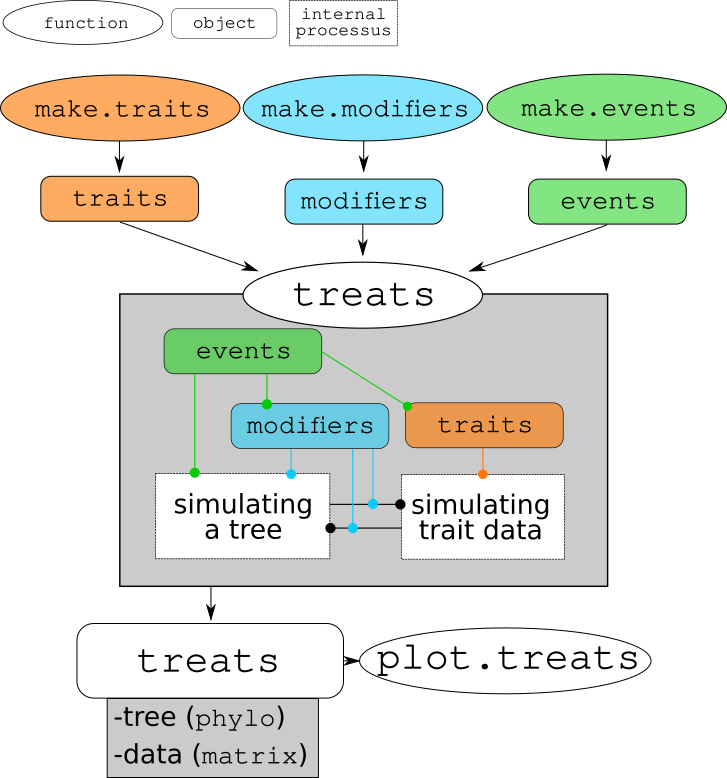
\includegraphics{treats_structure.png}
\caption{Schematic summary of the \texttt{treats} package architecture}
\end{figure}

\hypertarget{bdalgorithm}{%
\section{The birth-death algorithm}\label{bdalgorithm}}

\begin{quote}
If you want to get your hands dirty, you can go straight to the \protect\hyperlink{gettingstarted}{getting started section}, this following section just describes the process in pseudo-code.
\end{quote}

The \texttt{treats} algorithm is based on a modular version of the birth-death process algorithm.
The birth-death model is a continuous Markov process (i.e.~a continuous random process where future events depend only on the present, and not on past events) which is well defined mathematically and \href{https://lukejharmon.github.io/pcm/chapter10_birthdeath/\#section-10.2-the-birth-death-model}{commonly used in evolutionary biology} but also in \href{https://en.wikipedia.org/wiki/Birth\%E2\%80\%93death_process}{many other fields}.

The algorithm used in \texttt{treats} allows modularity of this process and is based on the following steps (the text in \texttt{courier\ font} is for the name of the process in the algorithm):

\begin{enumerate}
\def\labelenumi{\arabic{enumi}.}
\setcounter{enumi}{-1}
\tightlist
\item
  \textbf{Starting the process}: this step is non-modular and creates a random tree with one tip, one node and one branch connecting both. This step is used to optimise the rest of the algorithm in terms of speed and memory management. The node, tip and branch resulting from this step are discarded at the end of the simulations.
\item
  \textbf{Selecting a lineage} (\texttt{selecting}): this step selects a tip that is currently not extinct. In a standard birth-death process this is done randomly, however in \texttt{treats} this can be modified based on the birth-death parameters, the currently available lineages and potential trait values. \emph{For example, it is possible to put a higher probability for selecting a lineage that is closely related to a lineage that recently went extinct and has a positive trait value.}
  Then go to step 2.
\item
  \textbf{Growing the tree} (\texttt{waiting}): this step grows the tree by a certain amount. It does so by adding the same amount of branch length to all the non-extinct lineages. In an exact birth-death process, this is done by drawing a random value from an exponential distribution with a rate of \[\text{number of living lineages} \times (\text{speciation} + \text{extinction parameters})\]. In \texttt{treats}, this can be modified based on the birth-death parameters, the currently available lineages and potential trait values. \emph{For example, it is possible to increase branch length by the ratio of living/extinct fossils and a random number drawn from the range of current trait values.}
  If the total tree length is less than the required tree length, go to step 3. Else go to step 6.
\item
  \textbf{Simulating traits} {[}optional{]}(\texttt{traits}): this step allows you to simulate a trait value for the selected lineage from step 1. This is typically not part of a standard birth-death process and is handled via the \texttt{traits} option in \texttt{treats} (see the \protect\hyperlink{maketraits}{\texttt{make.traits}} chapter for more details).
  Then go to step 4.
\item
  \textbf{Speciating} (\texttt{speciating}): in this step, the selected lineage from step 1 has the option of speciating or going extinct. In a standard birth-death process, this happens by randomly drawing a value between 0 and 1 as a way to trigger speciation relative to the birth-death parameters:
\end{enumerate}

\begin{verbatim}
if
    randomly drawn number is smaller or equal to speciation/(speciation + extinction)
then
    do speciate
else
    go extinct
\end{verbatim}

Again, in \texttt{treats}, this process can be modified based on the birth-death parameters, the currently available lineages and potential trait values. \emph{For example, the lineage can only speciate if its trait value is positive, regardless of whether speciation or extinction have been triggered}.
Then go to step 5.
5. If the number of lineages is less than required number of lineages, then go to step 1. Else go to step 6.
6. The simulation stops because it has reached the required amount of lineages and/or time (i.e.~branch length).

\begin{verbatim}
## Loading required package: dispRity
\end{verbatim}

\hypertarget{gettingstarted}{%
\chapter{Getting started}\label{gettingstarted}}

\hypertarget{the-simplest-analysis-simulating-diversity-only}{%
\section{The simplest analysis: simulating diversity only}\label{the-simplest-analysis-simulating-diversity-only}}

One of the simplest things to do with the \texttt{treats} package is to simulate a birth-death tree.
For that you can use the function \texttt{treats} and specify your stopping rule.
The stopping rule simply tells the birth-death process to stop whenever it reaches one of these three conditions:

\begin{itemize}
\tightlist
\item
  \texttt{"max.taxa"\ \ \ =\ n} stop when \texttt{n} taxa are generated;
\item
  \texttt{"max.living"\ =\ n} stop when there are \texttt{n} co-occuring taxa of the same age (i.e.~``living'' taxa);
\item
  \texttt{"max.time"\ \ \ =\ n} stop when the simulated tree is \texttt{n} units of age old (these units are arbitrary);
\end{itemize}

For example, we might want to generate a birth-death tree with 20 taxa:

\begin{Shaded}
\begin{Highlighting}[]
\CommentTok{\#\# Setting a stopping rule to reach a maximum of 20 taxa}
\NormalTok{my\_stop\_rule \textless{}{-}}\StringTok{ }\KeywordTok{list}\NormalTok{(}\DataTypeTok{max.taxa =} \DecValTok{20}\NormalTok{)}
\end{Highlighting}
\end{Shaded}

We can now run the simulations using:

\begin{Shaded}
\begin{Highlighting}[]
\CommentTok{\#\# Running the birth{-}death simulation}
\NormalTok{my\_tree \textless{}{-}}\StringTok{ }\KeywordTok{treats}\NormalTok{(}\DataTypeTok{stop.rule =}\NormalTok{ my\_stop\_rule)}
\end{Highlighting}
\end{Shaded}

\begin{quote}
Note that here we could have specified more than one stopping rule, for example, we might want to run a simulation and stop it if it \emph{either} reaches 10 taxa \emph{or} the age 2 using \texttt{stop.rule\ =\ list(max.time\ =\ 2,\ max.taxa\ =\ 10)}. The simulation will then stop when either of these conditions are met.
\end{quote}

The resulting object is a classic \texttt{"phylo"} object that you can plot like so:

\begin{Shaded}
\begin{Highlighting}[]
\CommentTok{\#\# The tree object}
\NormalTok{my\_tree}
\end{Highlighting}
\end{Shaded}

\begin{verbatim}
## 
## Phylogenetic tree with 20 tips and 19 internal nodes.
## 
## Tip labels:
##   t1, t2, t3, t4, t5, t6, ...
## Node labels:
##   n1, n2, n3, n4, n5, n6, ...
## 
## Rooted; includes branch lengths.
\end{verbatim}

\begin{Shaded}
\begin{Highlighting}[]
\CommentTok{\#\# Plotting it}
\KeywordTok{plot}\NormalTok{(my\_tree)}
\end{Highlighting}
\end{Shaded}

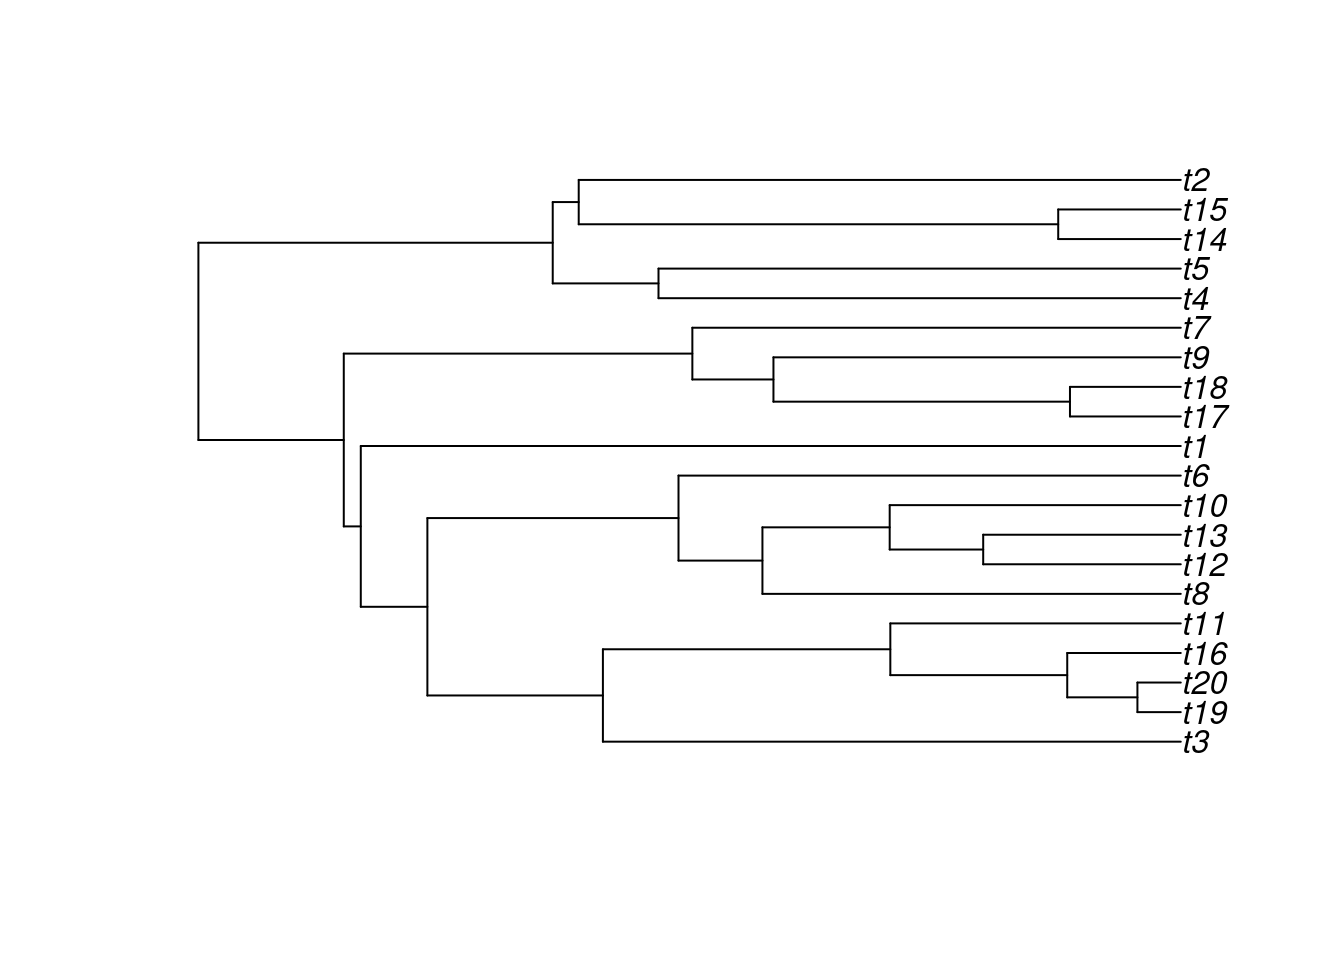
\includegraphics{treats_manual_files/figure-latex/unnamed-chunk-6-1.pdf}

\hypertarget{changing-the-birth-death-parameters}{%
\subsection{Changing the birth-death parameters}\label{changing-the-birth-death-parameters}}

People familiar with the \href{https://lukejharmon.github.io/pcm/chapter10_birthdeath/}{birth-death models} might have noticed that we did not specify two important things here: the speciation parameter (sometimes called ``lambda'' or ``birth'') and the extinction parameter (sometimes called ``mu'', ``death'' or ``background extinction'').
By default \texttt{treats} runs a pure birth model (speciation is set to 1 and extinction to 0).
However, you can easily change that by specifying your own birth-death parameters:

\begin{Shaded}
\begin{Highlighting}[]
\CommentTok{\#\# my birth{-}death parameters}
\NormalTok{my\_params \textless{}{-}}\StringTok{ }\KeywordTok{list}\NormalTok{(}\DataTypeTok{speciation =} \DecValTok{1}\NormalTok{,}
                  \DataTypeTok{extinction =} \DecValTok{1}\OperatorTok{/}\DecValTok{3}\NormalTok{)}
\end{Highlighting}
\end{Shaded}

\begin{quote}
You can find more information about setting up more complex birth-death parameters \protect\hyperlink{makebdparams}{in this section}.
\end{quote}

You can then run the same birth-death tree simulation with extinction:

\begin{Shaded}
\begin{Highlighting}[]
\CommentTok{\#\# Generating a birth{-}death tree with extinctions:}
\NormalTok{my\_tree \textless{}{-}}\StringTok{ }\KeywordTok{treats}\NormalTok{(}\DataTypeTok{bd.params =}\NormalTok{ my\_params, }\DataTypeTok{stop.rule =}\NormalTok{ my\_stop\_rule)}
\CommentTok{\#\# Visualising the new tree}
\KeywordTok{plot}\NormalTok{(my\_tree)}
\end{Highlighting}
\end{Shaded}

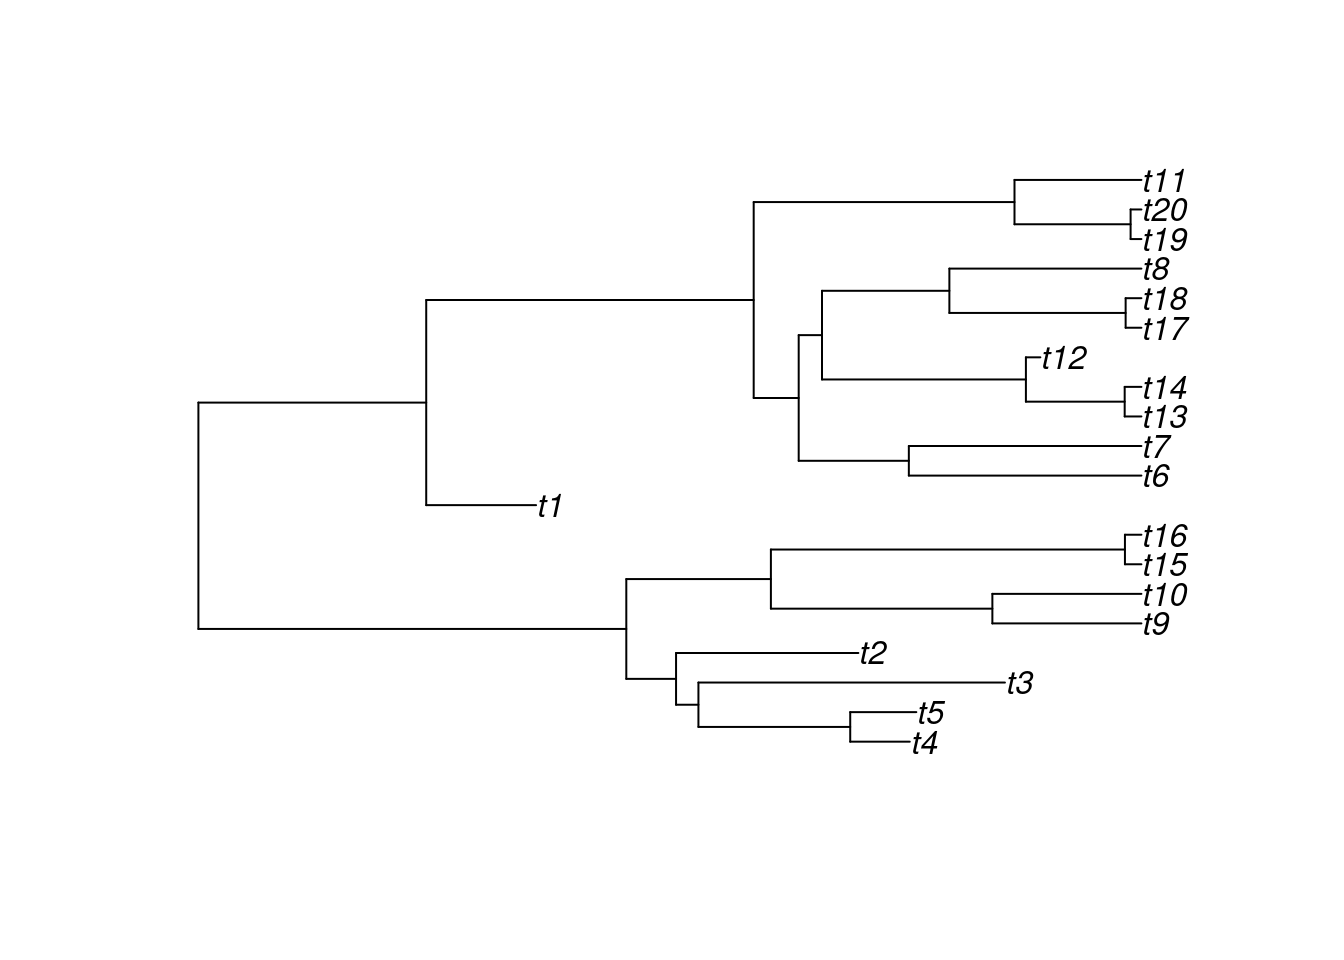
\includegraphics{treats_manual_files/figure-latex/unnamed-chunk-8-1.pdf}

\hypertarget{slightly-more-complex-simulating-disparity-and-diversity}{%
\section{Slightly more complex: simulating disparity and diversity}\label{slightly-more-complex-simulating-disparity-and-diversity}}

Chances are that you are using \texttt{treats} because you also want to simulate traits (disparity) along with your diversity (otherwise, we suggest using the \href{https://github.com/tanja819/TreeSim/}{\texttt{TreeSim}} package that provides many more birth-death models).
Simulating traits is not much more complicated in \texttt{treats}: you'll simply need to create a \texttt{"traits"} object using the \texttt{make.traits} function.
These objects can have increasing complexity (see the rest of this tutorial) but we will keep it simple here.

\texttt{"traits"} objects contain one or more processes which are the ways to generate the trait.
The most common of these processes is the \href{https://en.wikipedia.org/wiki/Brownian_motion}{Brownian Motion} model.
This is used by default with the \texttt{make.traits} function:

\begin{Shaded}
\begin{Highlighting}[]
\CommentTok{\#\# Creating the traits object}
\NormalTok{my\_trait \textless{}{-}}\StringTok{ }\KeywordTok{make.traits}\NormalTok{()}
\end{Highlighting}
\end{Shaded}

This trait object can be simply printed (to see what's in it) or plotted (to see what the process looks like in the absence of a phylogeny):

\begin{Shaded}
\begin{Highlighting}[]
\CommentTok{\#\# Which process is in here?}
\NormalTok{my\_trait}
\end{Highlighting}
\end{Shaded}

\begin{verbatim}
##  ---- treats traits object ---- 
## 1 trait for 1 process (A) with one starting value (0).
\end{verbatim}

\begin{Shaded}
\begin{Highlighting}[]
\CommentTok{\#\# What does it look like?}
\KeywordTok{plot}\NormalTok{(my\_trait)}
\end{Highlighting}
\end{Shaded}

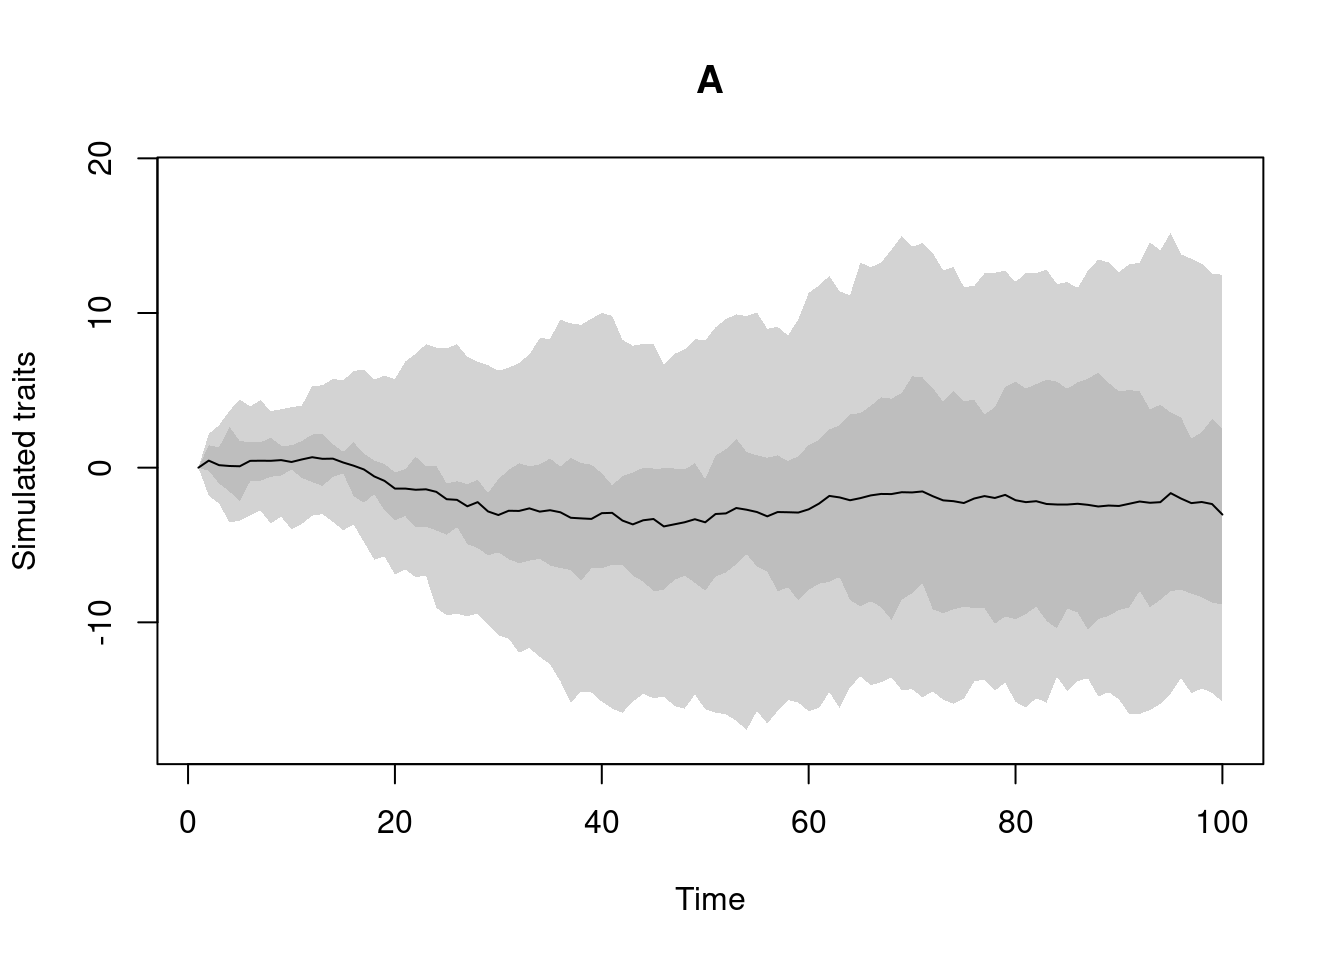
\includegraphics{treats_manual_files/figure-latex/unnamed-chunk-10-1.pdf}

By default, this trait is called ``A''.
This is not a really good name but you'll see more about specifying trait names later on.
If this is what the process should look like (theoretically) you can then add its \texttt{"traits"} object to our previous \texttt{treats} function to generate the tree and the traits:

\begin{Shaded}
\begin{Highlighting}[]
\CommentTok{\#\# Simulate disparity and diversity}
\NormalTok{my\_data \textless{}{-}}\StringTok{ }\KeywordTok{treats}\NormalTok{(}\DataTypeTok{bd.params =}\NormalTok{ my\_params,}
                \DataTypeTok{stop.rule =}\NormalTok{ my\_stop\_rule,}
                \DataTypeTok{traits    =}\NormalTok{ my\_trait)}
\end{Highlighting}
\end{Shaded}

Et voilà! We now have a simple disparity and diversity simulation.
We can see what's in the results by simply printing it or plotting it:

\begin{Shaded}
\begin{Highlighting}[]
\CommentTok{\#\# What\textquotesingle{}s in there}
\NormalTok{my\_data}
\end{Highlighting}
\end{Shaded}

\begin{verbatim}
##  ---- treats object ---- 
## Simulated phylogenetic tree (x$tree):
## 
## Phylogenetic tree with 20 tips and 19 internal nodes.
## 
## Tip labels:
##   t1, t2, t3, t4, t5, t6, ...
## Node labels:
##   n1, n2, n3, n4, n5, n6, ...
## 
## Rooted; includes branch lengths.
## 
## Simulated trait data (x$data):
## 1 trait for 1 process (A) with one starting value (0).
\end{verbatim}

\begin{Shaded}
\begin{Highlighting}[]
\CommentTok{\#\# Plotting the disparity and diversity}
\KeywordTok{plot}\NormalTok{(my\_data)}
\end{Highlighting}
\end{Shaded}

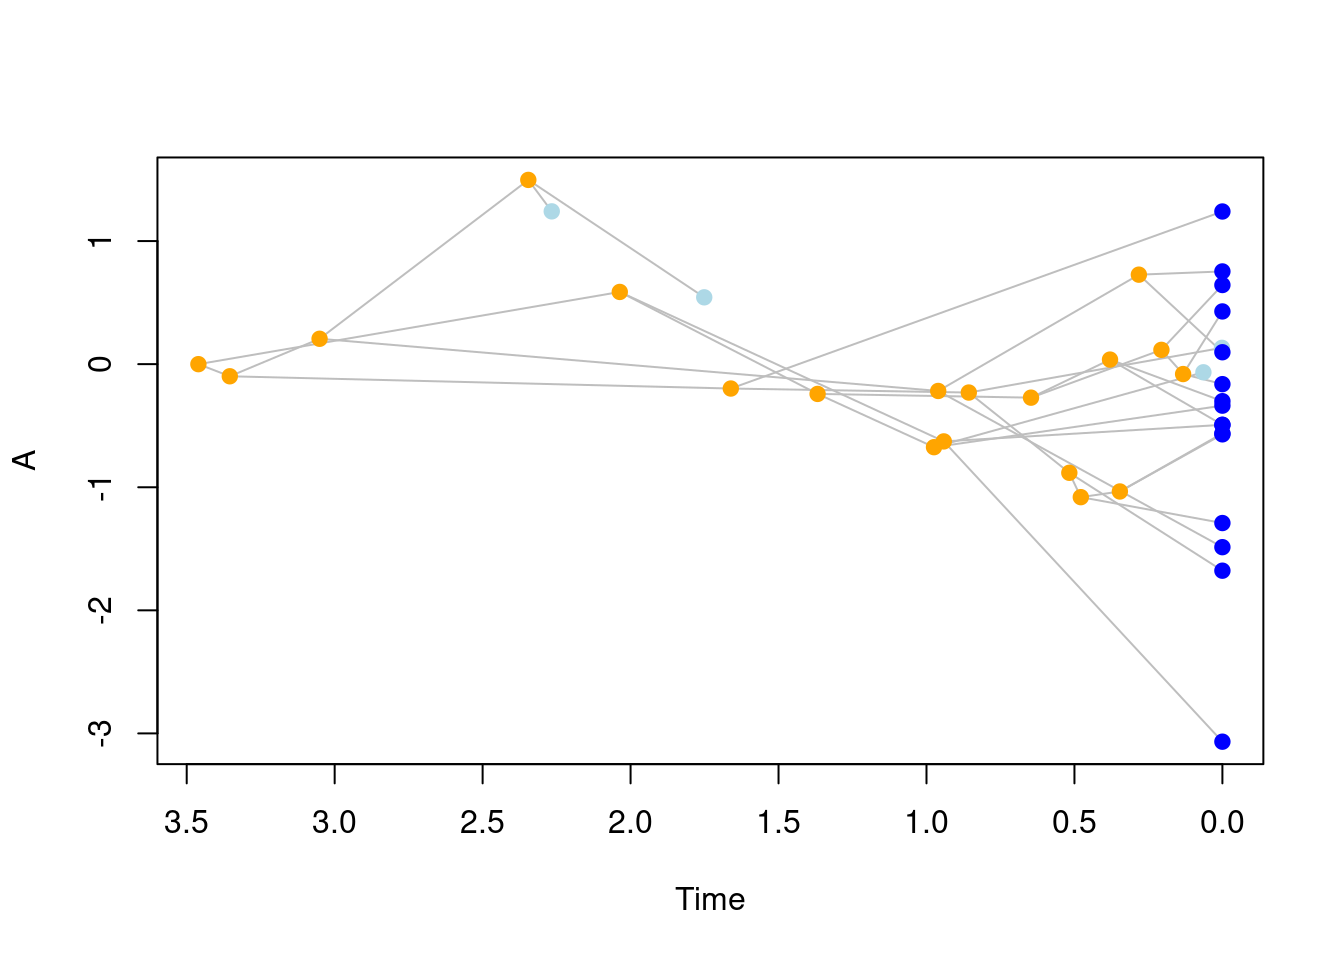
\includegraphics{treats_manual_files/figure-latex/unnamed-chunk-12-1.pdf}

You can then extract the components you need for your specific analysis like so:

\begin{Shaded}
\begin{Highlighting}[]
\CommentTok{\#\# Extracting the tree }
\NormalTok{the\_generated\_tree \textless{}{-}}\StringTok{ }\NormalTok{my\_data}\OperatorTok{$}\NormalTok{tree}
\CommentTok{\# Note that this is a "phylo" object}
\KeywordTok{class}\NormalTok{(the\_generated\_tree)}
\end{Highlighting}
\end{Shaded}

\begin{verbatim}
## [1] "phylo"
\end{verbatim}

\begin{Shaded}
\begin{Highlighting}[]
\CommentTok{\#\# Extracting the data }
\NormalTok{the\_generated\_data \textless{}{-}}\StringTok{ }\NormalTok{my\_data}\OperatorTok{$}\NormalTok{data}
\CommentTok{\# Note that this is a "matrix" or "array"}
\KeywordTok{class}\NormalTok{(the\_generated\_data)}
\end{Highlighting}
\end{Shaded}

\begin{verbatim}
## [1] "matrix" "array"
\end{verbatim}

You can find much more about how to design trait objects in the \protect\hyperlink{maketraits}{\texttt{make.traits} section}.

\hypertarget{treats-objects}{%
\subsection{\texorpdfstring{\texttt{"treats"} objects}{"treats" objects}}\label{treats-objects}}

\texttt{treats} will output either just a tree (class \texttt{"phylo"}) if no traits were generated or a \texttt{"treats"} object that contains both a \texttt{\$tree} (\texttt{"phylo"}) and a \texttt{\$data} (\texttt{"matrix"}) component.
Note that this \texttt{"treats"} class is generalised to most outputs of the package functions.
This allows for a smoother handeling of the objects outputs such as summarising the content of a \texttt{make.bd.params} output or visualising a trait output from \texttt{make.traits}.

\hypertarget{slightly-more-complex-again-simulating-linked-disparity-and-diversity}{%
\section{Slightly more complex again: simulating linked disparity and diversity}\label{slightly-more-complex-again-simulating-linked-disparity-and-diversity}}

The example above is still pretty simple and easily done through a variety of \texttt{R} packages: here the trait and the tree are simulated at the same time but only the tree is simulating the trait (i.e.~the trait value at a tip is affected by its ancestor and the branch length leading to it) but not the other way around (the trait value does not affect the tree).
It is possible to add this aspect using \texttt{"modifiers"} objects.
\texttt{"modifiers"} are similar to \texttt{"traits"} in that you specify what should go in there and then feed it to your simulation.

\texttt{"modifiers"} affect two key steps of the birth-death process: the calculation of the waiting time (i.e.~the component generating branch lengths) and the triggering of speciation or extinction events.
These events can be modified using \texttt{condition} and \texttt{modify} functions.
In other words, when reaching a certain condition specified by a \texttt{condition} function, the birth-death process will modify either the branch length or the speciation (or extinction) probability by applying a \texttt{modify} function.

You can use the function \texttt{make.modifiers} to design a specific \texttt{"modifiers"} object.
By default, this function generates a \texttt{"modifiers"} object that affects branch length and speciation in the following way:

\begin{itemize}
\tightlist
\item
  branch length is a randomly drawn number from an exponential distribution with a rate equal to the current number of taxa multiplied by the sum of the speciation and extinction rates.
\item
  speciation is triggered if a randomly drawn number (from a (0,1) uniform distribution) is smaller than the ratio between the speciation rate and the sum of the speciation and extinction rates. If that random number is greater, the lineage goes extinct.
\end{itemize}

Note that these are defaults for a birth-death tree and were already applied in the examples above without specifying a \texttt{"modifiers"} object:

\begin{Shaded}
\begin{Highlighting}[]
\CommentTok{\#\# Make a default modifiers object}
\NormalTok{default\_modifiers \textless{}{-}}\StringTok{ }\KeywordTok{make.modifiers}\NormalTok{()}
\CommentTok{\#\# What\textquotesingle{}s in it?}
\NormalTok{default\_modifiers}
\end{Highlighting}
\end{Shaded}

\begin{verbatim}
##  ---- treats modifiers object ---- 
## No modifiers applied to the branch length, selection and speciation processes (default).
\end{verbatim}

This will not do anything to our simulations compared to the previous trait and tree simulation but we can provide our \texttt{"modifiers"} object to the \texttt{treats} function:

\begin{Shaded}
\begin{Highlighting}[]
\CommentTok{\#\# Setting the simulation parameters}
\NormalTok{extinction\_}\DecValTok{02}\NormalTok{ \textless{}{-}}\StringTok{ }\KeywordTok{list}\NormalTok{(}\DataTypeTok{extinction =} \FloatTok{0.2}\NormalTok{)}
\NormalTok{living\_}\DecValTok{20}\NormalTok{     \textless{}{-}}\StringTok{ }\KeywordTok{list}\NormalTok{(}\DataTypeTok{max.living =} \DecValTok{20}\NormalTok{)}
\NormalTok{BM\_trait      \textless{}{-}}\StringTok{ }\KeywordTok{make.traits}\NormalTok{()}

\CommentTok{\# Set random seed so we get the same results}
\KeywordTok{set.seed}\NormalTok{(}\DecValTok{1}\NormalTok{)}

\CommentTok{\#\# Simulate disparity and diversity}
\NormalTok{default\_data \textless{}{-}}\StringTok{ }\KeywordTok{treats}\NormalTok{(}\DataTypeTok{bd.params =}\NormalTok{ extinction\_}\DecValTok{02}\NormalTok{,}
                     \DataTypeTok{stop.rule =}\NormalTok{ living\_}\DecValTok{20}\NormalTok{,}
                     \DataTypeTok{traits    =}\NormalTok{ BM\_trait,}
                     \DataTypeTok{modifiers =}\NormalTok{ default\_modifiers)}
\NormalTok{default\_data}
\end{Highlighting}
\end{Shaded}

\begin{verbatim}
##  ---- treats object ---- 
## Birth death process with modifiers:
## speciation: 1.
## extinction: 0.2.
## No modifiers applied to the branch length, selection and speciation processes (default).
## Simulated phylogenetic tree (x$tree):
## 
## Phylogenetic tree with 24 tips and 23 internal nodes.
## 
## Tip labels:
##   t1, t2, t3, t4, t5, t6, ...
## Node labels:
##   n1, n2, n3, n4, n5, n6, ...
## 
## Rooted; includes branch lengths.
## 
## Simulated trait data (x$data):
## 1 trait for 1 process (A) with one starting value (0).
\end{verbatim}

Note however, that the printing information is now updated to state that you've added a \texttt{"modifiers"} object (even though it's the same as the default).
In this specific case the \texttt{modifiers} object is not necessary as it is doing nothing different than when using the default one (i.e.~when no \texttt{modifiers} is provided).

For more interesting simulations however, you can provide modifiers that actually modify the birth-death process.
We can create one for example that makes species go extinct if their ancestor has a negative trait value.
For that we need to create a \texttt{"modifiers"} object that modifies the \texttt{speciation} process with a specific condition and a specific modification when that condition is met.
For a speciation to occur (and a species to not go extinct), the algorithm draws a random value \emph{x} between 0 and 1 and if the value is smaller than the speciation parameter divided by the speciation + extinction parameter, the lineage speciates (\(x < (\lambda \div (\lambda + \mu))\)), else it goes extinct.
\emph{x} is a random value that simulates some stochasticity in the evolutionary simulation.
At every step of the simulation, a different random value \emph{x} is drawn making sure that the resulting speciation or extinction is not predictable.

However, we can create a modifier that introduces less randomness (or a different level of randomness) by forcing the lineage to go extinct every time a specific condition is met, e.g.~if the lineage trait value is negative.
This can be done for example by not randomly generating the value \emph{x} but giving it a fixed value of say 1 so that the estimation of the speciation function \(x < (\lambda \div (\lambda + \mu))\) is always met.
In other words, if the lineage's trait value is negative, make sure that \emph{x} is equal to 1, so that the speciation condition \(x < (\lambda \div\ (\lambda + \mu))\) is never met.

First we need to create a \texttt{condition} function to trigger this (non) speciation event.
We can do that by specifying our \texttt{condition} function (here the \texttt{going.extinct} function) to apply our modification.
For that we can use the \texttt{parent.traits} utility function that is optimised for accessing traits in the birth-death process (but you can of course write your own).
This function takes the \texttt{trait.values} and \texttt{parent.lineage} arguments, two arguments that you can leave named as they are to facilitate \texttt{treats}' understanding of what you want to assess:

\begin{Shaded}
\begin{Highlighting}[]
\CommentTok{\#\# Triggering a modification only if the ancestor trait is negative}
\NormalTok{negative.ancestor \textless{}{-}}\StringTok{ }\ControlFlowTok{function}\NormalTok{(trait.values, lineage) \{}
    \KeywordTok{return}\NormalTok{(}\KeywordTok{all}\NormalTok{(}\KeywordTok{parent.traits}\NormalTok{(trait.values, lineage) }\OperatorTok{\textless{}}\StringTok{ }\DecValTok{0}\NormalTok{))}
\NormalTok{\}}
\end{Highlighting}
\end{Shaded}

\begin{quote}
Note that we use the function \texttt{all} here to evaluate all traits: i.e.~if the data has more than one trait we trigger the modification only if all the trait values are negative.
\end{quote}

Then we create the modification function.
This function must take the argument \texttt{x} and, in our case, returns the same value no matter what: \texttt{1} so that speciation never happens when the \texttt{negative.ancestor} function is triggered.

\begin{Shaded}
\begin{Highlighting}[]
\CommentTok{\#\# Always go extinct}
\NormalTok{going.extinct \textless{}{-}}\StringTok{ }\ControlFlowTok{function}\NormalTok{(x) }\KeywordTok{return}\NormalTok{(}\DecValTok{1}\NormalTok{)}
\end{Highlighting}
\end{Shaded}

This \texttt{going.extinct} function is to be contrasted with the normal modifier for selecting the value \texttt{x} which is \texttt{runif(1)} (drawing a random value between 0 and 1).
We can then provide these two functions (the condition \texttt{negative.ancestor} and how to modify the speciation event when this condition is met \texttt{going.extinct}).
If you are an advances \texttt{treats} user, you can design your own \texttt{speciation} function but if you just want to use a normal \texttt{speciation} function, you can use the default one from \texttt{treats} called \texttt{speciation}.

\begin{Shaded}
\begin{Highlighting}[]
\CommentTok{\#\# Making a modifier for species to go extinct if}
\CommentTok{\#\# their ancestor\textquotesingle{}s trait value is (or are) negative}
\NormalTok{negatives\_extinct \textless{}{-}}\StringTok{ }\KeywordTok{make.modifiers}\NormalTok{(}
            \CommentTok{\#\# If the following condition is met...}
            \DataTypeTok{condition =}\NormalTok{ negative.ancestor, }\CommentTok{\# Does the lineage have an ancestor with negative trait values?}
            \CommentTok{\#\# Then apply the following modifier...}
            \DataTypeTok{modify =}\NormalTok{ going.extinct, }\CommentTok{\# The species goes extinct}
            \CommentTok{\#\# To the the speciation process.}
            \DataTypeTok{speciation =}\NormalTok{ speciation) }\CommentTok{\# Here the speciation() process is default}

\CommentTok{\#\# What\textquotesingle{}s in it?}
\NormalTok{negatives\_extinct}
\end{Highlighting}
\end{Shaded}

\begin{verbatim}
##  ---- treats modifiers object ---- 
## Default branch length process.
## Default selection process.
## Speciation process is set to speciation with a condition (negative.ancestor) and a modifier (going.extinct).
\end{verbatim}

Note that the \texttt{make.modifiers} function tests whether the input is compatible with \texttt{treats} by default so unless you have an error message, your \texttt{modifiers} will work!
We can now simulate our tree and traits with our modifier: species will go extinct if their ancestor has a negative trait value:

\begin{Shaded}
\begin{Highlighting}[]
\KeywordTok{set.seed}\NormalTok{(}\DecValTok{1}\NormalTok{)}
\CommentTok{\#\# Simulate disparity and diversity}
\NormalTok{modified\_data \textless{}{-}}\StringTok{ }\KeywordTok{treats}\NormalTok{(}\DataTypeTok{bd.params =}\NormalTok{ extinction\_}\DecValTok{02}\NormalTok{,}
                        \DataTypeTok{stop.rule =}\NormalTok{ living\_}\DecValTok{20}\NormalTok{,}
                        \DataTypeTok{traits    =}\NormalTok{ BM\_trait,}
                        \DataTypeTok{modifiers =}\NormalTok{ negatives\_extinct)}
\NormalTok{modified\_data}
\end{Highlighting}
\end{Shaded}

\begin{verbatim}
##  ---- treats object ---- 
## Birth death process with modifiers:
## speciation: 1.
## extinction: 0.2.
## Default branch length process.
## Default selection process.
## Speciation process is set to speciation with a condition (negative.ancestor) and a modifier (going.extinct).
## Simulated phylogenetic tree (x$tree):
## 
## Phylogenetic tree with 22 tips and 21 internal nodes.
## 
## Tip labels:
##   t1, t2, t3, t4, t5, t6, ...
## Node labels:
##   n1, n2, n3, n4, n5, n6, ...
## 
## Rooted; includes branch lengths.
## 
## Simulated trait data (x$data):
## 1 trait for 1 process (A) with one starting value (0).
\end{verbatim}

We can now compare the two trees and their trait values.
Note that we've used the same starting seed for both trees so the only thing differing between them is the \texttt{"modifier"} object which leads to very different trees!

\begin{Shaded}
\begin{Highlighting}[]
\KeywordTok{par}\NormalTok{(}\DataTypeTok{mfrow =} \KeywordTok{c}\NormalTok{(}\DecValTok{1}\NormalTok{,}\DecValTok{2}\NormalTok{))}
\KeywordTok{plot}\NormalTok{(default\_data, }\DataTypeTok{main =} \StringTok{"default results"}\NormalTok{)}
\KeywordTok{plot}\NormalTok{(modified\_data, }\DataTypeTok{main =} \StringTok{"results with the modifier"}\NormalTok{)}
\end{Highlighting}
\end{Shaded}

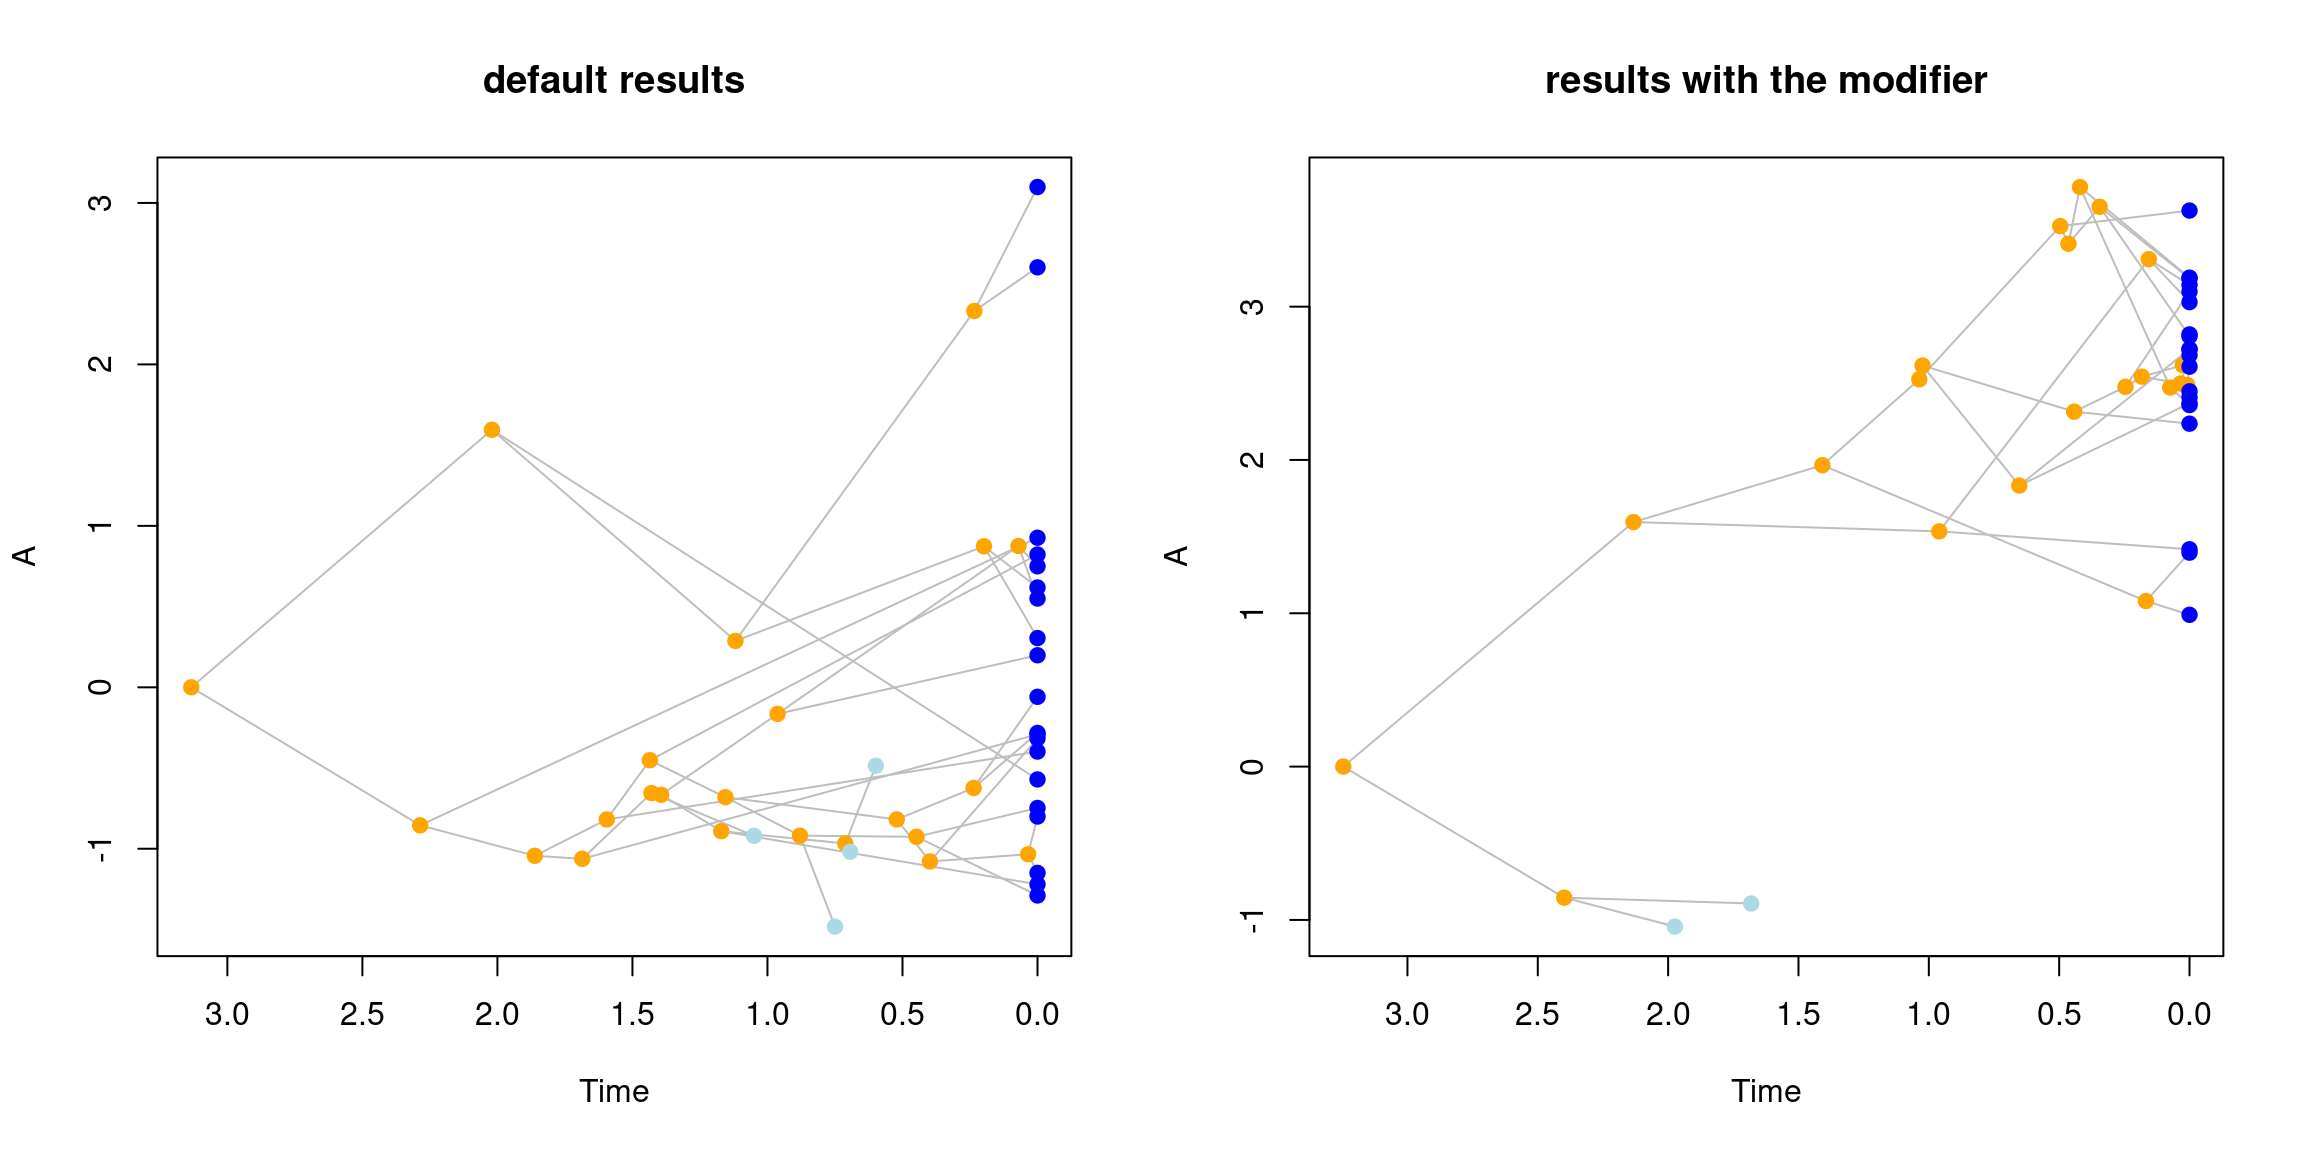
\includegraphics{treats_manual_files/figure-latex/unnamed-chunk-20-1.pdf}

You can find much more about how to design modifiers in the \protect\hyperlink{makemodifiers}{\texttt{make.modifiers} section}.

\hypertarget{kpgexample}{%
\section{An illustrative example: mammals disparity through the K-Pg extinction}\label{kpgexample}}

Bib is studying the evolution of mammalian disparity (i.e.~diversity of shapes) across the Cretaceous-Palaeogene mass extinction event (K-Pg - 66 million years ago).

They use a dataset from \citet{beckancient2014} that is a discrete morphological space containing the ordination of the around 400 morphological characters for 50 species and estimated for their 49 descendants into an ordinated shapespace of 99 elements and 97 dimensions.

\begin{Shaded}
\begin{Highlighting}[]
\KeywordTok{library}\NormalTok{(dispRity)}
\CommentTok{\#\# Loading the mammalian morphological example data}
\KeywordTok{data}\NormalTok{(BeckLee\_mat99)}

\CommentTok{\#\# This is what the dataset looks like}
\KeywordTok{head}\NormalTok{(BeckLee\_mat99)[}\DecValTok{1}\OperatorTok{:}\DecValTok{5}\NormalTok{, }\DecValTok{1}\OperatorTok{:}\DecValTok{5}\NormalTok{]}
\end{Highlighting}
\end{Shaded}

\begin{verbatim}
##                   [,1]        [,2]        [,3]       [,4]        [,5]
## Cimolestes  -0.6794737  0.15658591  0.04918307  0.2250983 -0.38139436
## Maelestes   -0.5797289  0.04223105 -0.20329542 -0.1545388 -0.06993258
## Batodon     -0.8812102  0.33619889  0.41748560  0.2446872 -0.31922156
## Bulaklestes -0.9295090 -0.08517626  0.11364659  0.3589646 -0.54998508
## Daulestes   -1.0025229 -0.09260779  0.06354371  0.4614256 -0.61211569
\end{verbatim}

And a tree showing the relation between these species through time:

\begin{Shaded}
\begin{Highlighting}[]
\CommentTok{\#\# The phylogenetic tree}
\KeywordTok{data}\NormalTok{(BeckLee\_tree)}

\CommentTok{\#\# And what the tree looks like}
\KeywordTok{plot}\NormalTok{(BeckLee\_tree, }\DataTypeTok{cex =} \FloatTok{0.8}\NormalTok{)}
\KeywordTok{axisPhylo}\NormalTok{()}
\KeywordTok{abline}\NormalTok{(}\DataTypeTok{v =}\NormalTok{ BeckLee\_tree}\OperatorTok{$}\NormalTok{root.time }\OperatorTok{{-}}\StringTok{ }\DecValTok{66}\NormalTok{, }\DataTypeTok{col =} \StringTok{"red"}\NormalTok{)}
\end{Highlighting}
\end{Shaded}

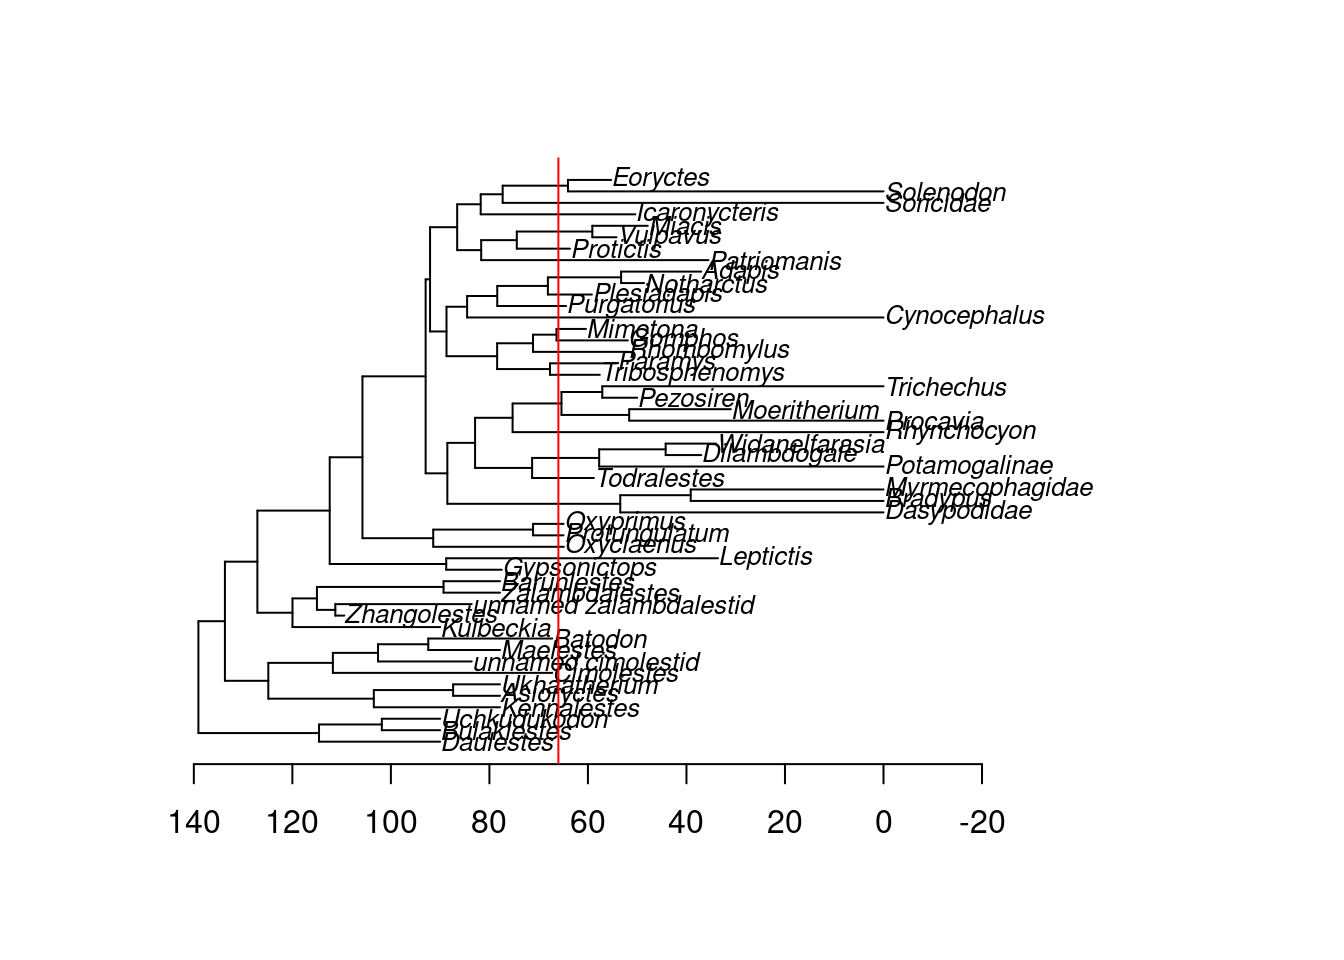
\includegraphics{treats_manual_files/figure-latex/unnamed-chunk-22-1.pdf}

They measure the disparity as the sum of variances as a proxy for changes in the traitspace size (\citet{moms}) with some bootstrapping to create some confidence intervals around that curve.

\begin{Shaded}
\begin{Highlighting}[]
\CommentTok{\#\# Making continuous time series}
\NormalTok{time\_series \textless{}{-}}\StringTok{ }\KeywordTok{chrono.subsets}\NormalTok{(}\DataTypeTok{data =}\NormalTok{ BeckLee\_mat99,}
                              \DataTypeTok{tree =}\NormalTok{ BeckLee\_tree,}
                              \DataTypeTok{method =} \StringTok{"continuous"}\NormalTok{, }\DataTypeTok{model =} \StringTok{"proximity"}\NormalTok{,}
                              \DataTypeTok{time =} \KeywordTok{seq}\NormalTok{(}\DataTypeTok{from =} \DecValTok{101}\NormalTok{, }\DataTypeTok{to =} \DecValTok{41}\NormalTok{, }\DataTypeTok{by =} \DecValTok{{-}5}\NormalTok{))}
\CommentTok{\#\# Calculating disparity}
\NormalTok{change\_in\_size \textless{}{-}}\StringTok{ }\KeywordTok{dispRity}\NormalTok{(}\KeywordTok{boot.matrix}\NormalTok{(time\_series), }\DataTypeTok{metric =} \KeywordTok{c}\NormalTok{(sum, variances))}
\KeywordTok{plot}\NormalTok{(change\_in\_size)}
\KeywordTok{abline}\NormalTok{(}\DataTypeTok{v =} \DecValTok{8}\NormalTok{, }\DataTypeTok{col =} \StringTok{"red"}\NormalTok{)}
\end{Highlighting}
\end{Shaded}

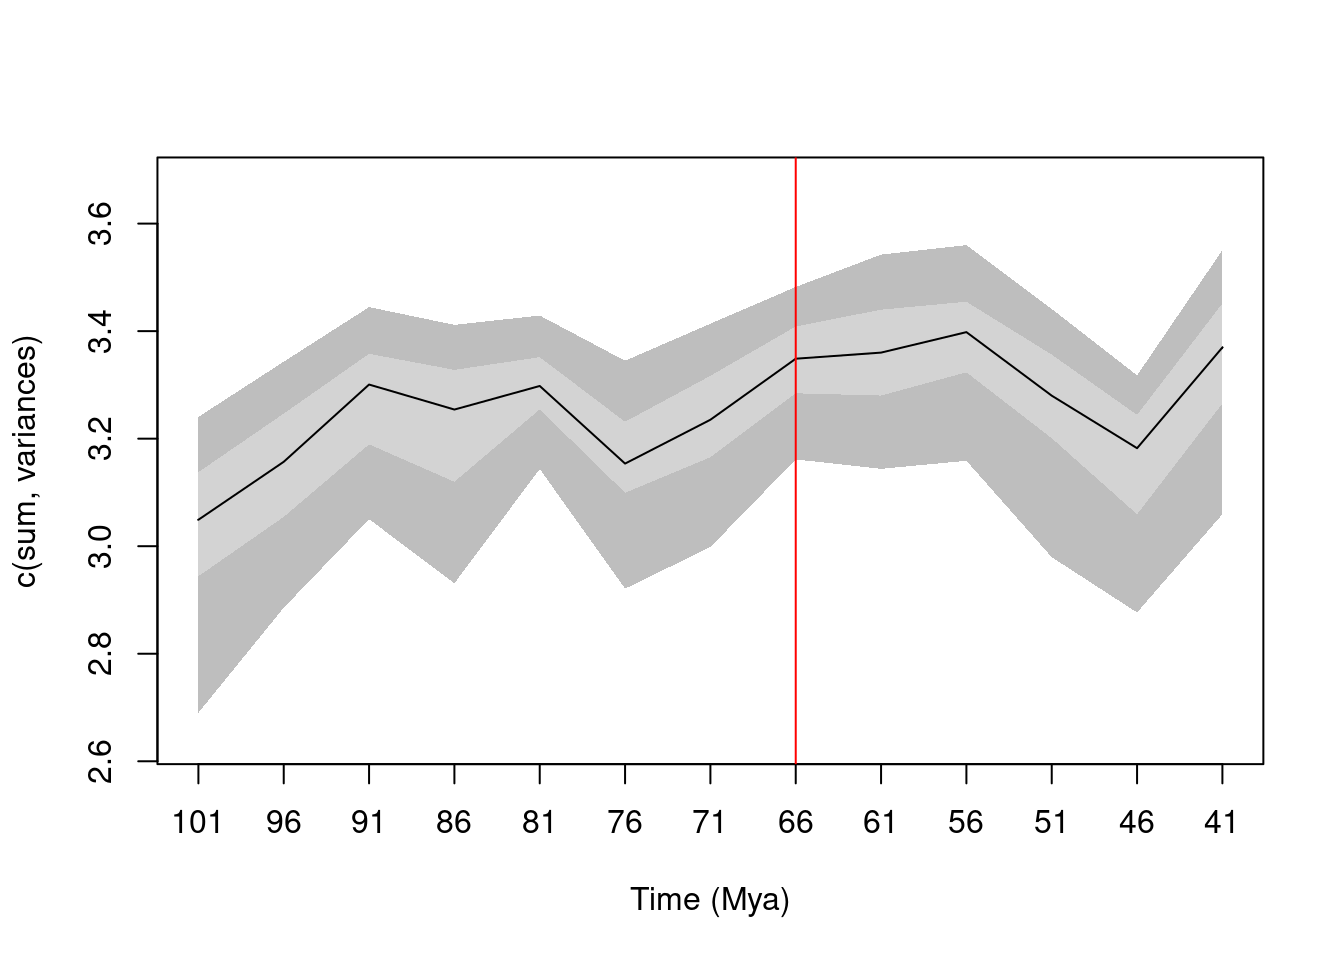
\includegraphics{treats_manual_files/figure-latex/unnamed-chunk-23-1.pdf}

\begin{quote}
For more info about \texttt{chrono.subsets} and the \texttt{dispRity} package, you can have a look at the \href{http://tguillerme.github.io/dispRity.html}{\texttt{dispRity} manual}.
\end{quote}

Looking at this curve, Bib wants to know whether disparity increased as a response to the K-Pg mass extinction or not.
To do this, they need to check whether changes in disparity can actually be detected due to an extinction event (e.g.~if an extinction event happens, does that change disparity curves?).
As a subsidiary question, they want to know whether the pattern is more likely due to a selective or random extinction event.

\hypertarget{simulating-trees-and-traits-using-the-observed-parameters}{%
\subsection{Simulating trees and traits using the observed parameters}\label{simulating-trees-and-traits-using-the-observed-parameters}}

The first step is to simulate the observed tree.
We can do that by using crude parameters from the observed tree:

\begin{Shaded}
\begin{Highlighting}[]
\CommentTok{\#\# Extracting the crude parameters}
\NormalTok{(est\_params \textless{}{-}}\StringTok{ }\KeywordTok{crude.bd.est}\NormalTok{(BeckLee\_tree, }\DataTypeTok{method =} \StringTok{"count"}\NormalTok{))}
\end{Highlighting}
\end{Shaded}

\begin{verbatim}
##  ---- treats birth-death parameters object ---- 
## speciation: 0.028.
## extinction: 0.027.
\end{verbatim}

\begin{Shaded}
\begin{Highlighting}[]
\CommentTok{\#\# These parameters are the observed speciation and extinction rate per million years.}

\CommentTok{\#\# Setting the stopping rule (stop after reaching 50 taxa)}
\NormalTok{stop\_rule \textless{}{-}}\StringTok{ }\KeywordTok{list}\NormalTok{(}\DataTypeTok{max.taxa =} \DecValTok{50}\NormalTok{)}

\CommentTok{\#\# Simulating just a birth{-}death tree with these parameters to check}
\KeywordTok{set.seed}\NormalTok{(}\DecValTok{1}\NormalTok{)}
\NormalTok{test\_tree \textless{}{-}}\StringTok{ }\KeywordTok{treats}\NormalTok{(}\DataTypeTok{bd.params  =}\NormalTok{ est\_params,}
                    \DataTypeTok{stop.rule  =}\NormalTok{ stop\_rule,}
                    \DataTypeTok{null.error =} \DecValTok{100}\NormalTok{)}
\end{Highlighting}
\end{Shaded}

\begin{verbatim}
## Building the tree:.Done.
\end{verbatim}

\begin{Shaded}
\begin{Highlighting}[]
\KeywordTok{plot}\NormalTok{(}\KeywordTok{ladderize}\NormalTok{(test\_tree), }\DataTypeTok{cex =} \FloatTok{0.8}\NormalTok{)}
\KeywordTok{axisPhylo}\NormalTok{()}
\end{Highlighting}
\end{Shaded}

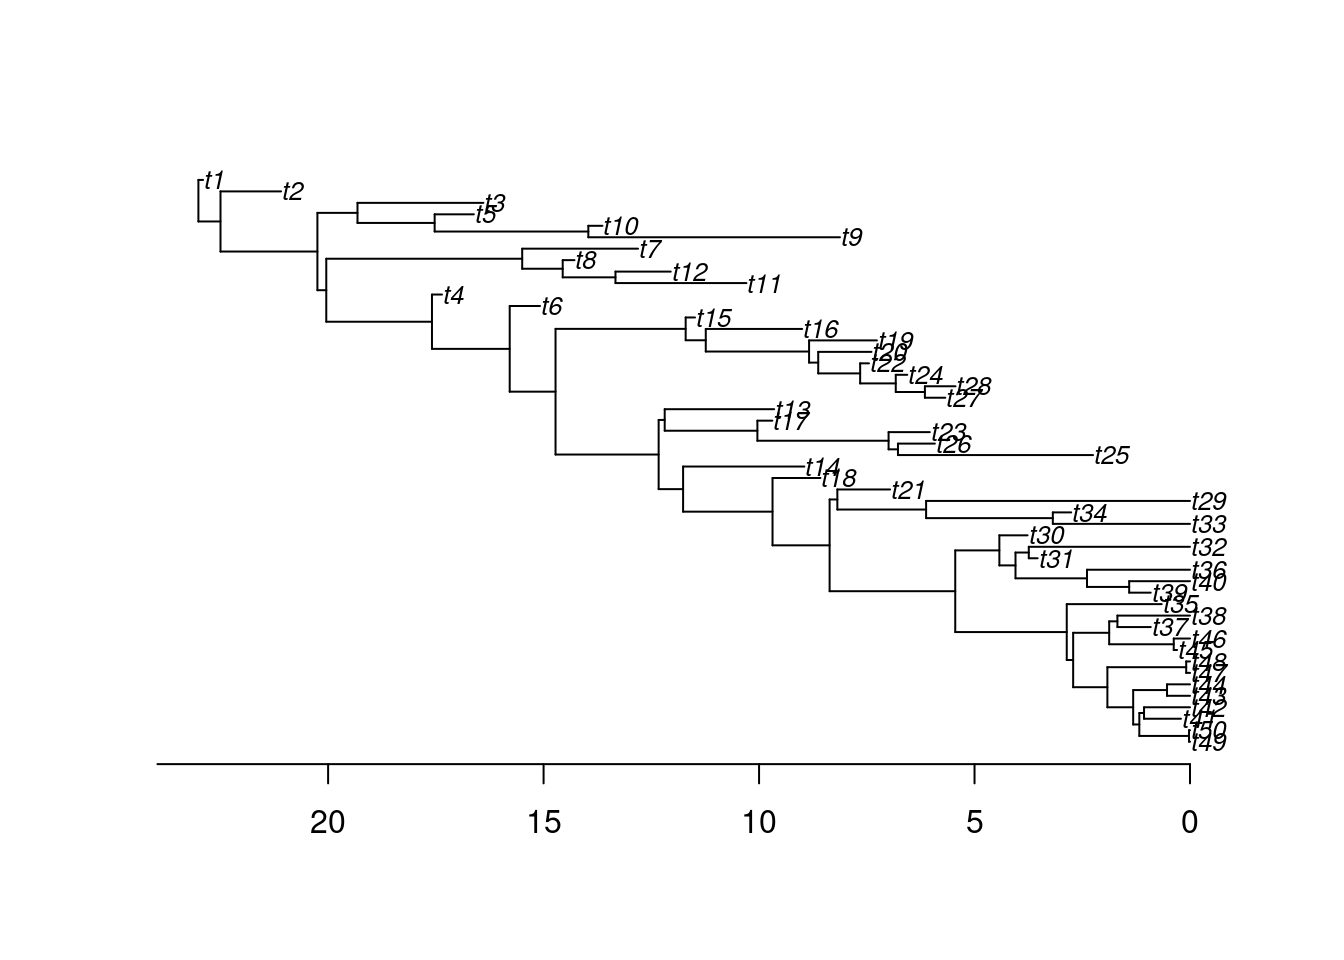
\includegraphics{treats_manual_files/figure-latex/unnamed-chunk-24-1.pdf}

\begin{quote}
Note that because of the high extinction to speciation ratio, the tree simulations can often fail before reaching the stop rule (i.e.~all lineages go extinct before reaching 50 taxa). To avoid getting stuck in there, we use the option \texttt{null.error\ =\ 100} to rerun the simulations up to 100 times before obtaining a tree that did not went fully extinct. Also note that using such parameters make the simulations run slowlier but ensure the requested results are always achieved.
\end{quote}

We now have a way to simulate a topology close to the observed one. We can simulate a list of topologies by replicating this function X amounts of time to get a distribution of trees:

\begin{Shaded}
\begin{Highlighting}[]
\CommentTok{\#\# Generating 50 trees}
\NormalTok{tree\_distribution \textless{}{-}}\StringTok{ }\KeywordTok{treats}\NormalTok{(}\DataTypeTok{bd.params  =}\NormalTok{ est\_params,}
                            \DataTypeTok{stop.rule  =}\NormalTok{ stop\_rule,}
                            \DataTypeTok{null.error =} \DecValTok{100}\NormalTok{,}
                            \DataTypeTok{replicates =} \DecValTok{50}\NormalTok{)}
\end{Highlighting}
\end{Shaded}

Of course, here our objective is to also simulate some trait values to measure disparity under some simulated scenario.
We can do that be adding a \texttt{"traits"} object to the \texttt{treats} function.
Here we will use a default \href{https://en.wikipedia.org/wiki/Brownian_motion}{Brownian Motion} to simulate our trait.

\begin{Shaded}
\begin{Highlighting}[]
\CommentTok{\#\# Creating a trait in 97 dimensions.}
\NormalTok{my\_traits \textless{}{-}}\StringTok{ }\KeywordTok{make.traits}\NormalTok{(}\DataTypeTok{process =}\NormalTok{ BM.process, }\DataTypeTok{n =} \KeywordTok{ncol}\NormalTok{(BeckLee\_mat99))}
\end{Highlighting}
\end{Shaded}

\begin{quote}
Note that there are many more options on how to simulate your trait such as using correlation, different processes, etc\ldots{} See details in the \protect\hyperlink{maketraits}{make traits section}.
\end{quote}

\begin{Shaded}
\begin{Highlighting}[]
\CommentTok{\#\# Simulate the tree and traits}
\NormalTok{sim\_data \textless{}{-}}\StringTok{ }\KeywordTok{treats}\NormalTok{(}\DataTypeTok{traits     =}\NormalTok{ my\_traits,}
                   \DataTypeTok{bd.params  =}\NormalTok{ est\_params,}
                   \DataTypeTok{stop.rule  =}\NormalTok{ stop\_rule,}
                   \DataTypeTok{null.error =} \DecValTok{100}\NormalTok{)}
\end{Highlighting}
\end{Shaded}

We can visualise the resulting tree using the \texttt{plot} function and visualising the different traits using the \texttt{trait} option in \texttt{plot}:

\begin{Shaded}
\begin{Highlighting}[]
\CommentTok{\#\# Plotting the results (first trait)}
\KeywordTok{plot}\NormalTok{(sim\_data, }\DataTypeTok{trait =} \DecValTok{1}\NormalTok{)}
\end{Highlighting}
\end{Shaded}

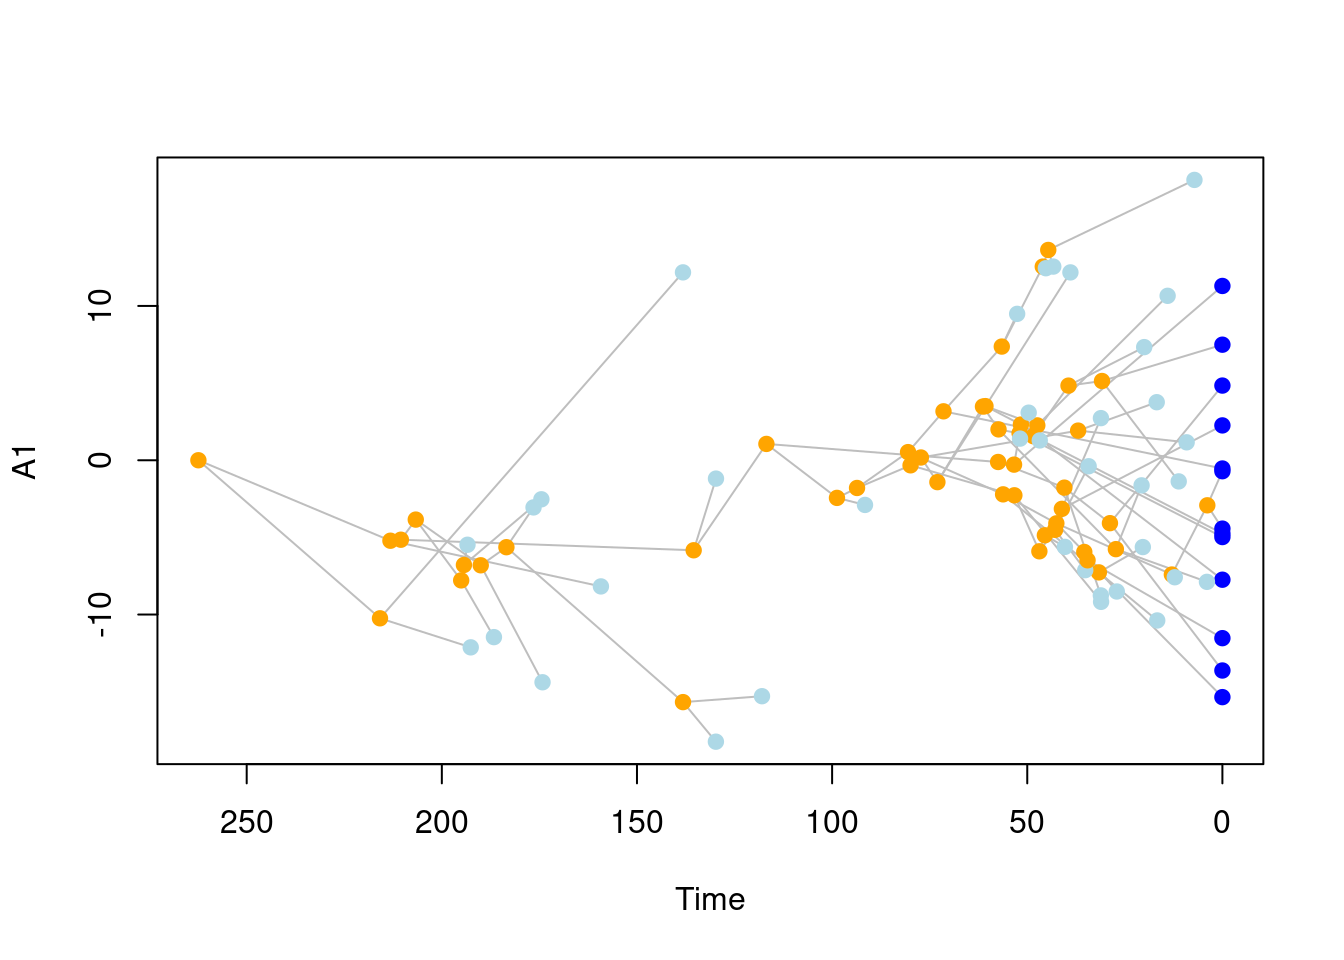
\includegraphics{treats_manual_files/figure-latex/unnamed-chunk-28-1.pdf}

Of course, here we want to simulate a distribution of trees and traits:

\begin{Shaded}
\begin{Highlighting}[]
\CommentTok{\#\# Simulate the tree and traits}
\NormalTok{sim\_data \textless{}{-}}\StringTok{ }\KeywordTok{treats}\NormalTok{(}\DataTypeTok{traits     =}\NormalTok{ my\_traits,}
                   \DataTypeTok{bd.params  =}\NormalTok{ est\_params,}
                   \DataTypeTok{stop.rule  =}\NormalTok{ stop\_rule,}
                   \DataTypeTok{null.error =} \DecValTok{100}\NormalTok{,}
                   \DataTypeTok{replicates =} \DecValTok{50}\NormalTok{)}
\end{Highlighting}
\end{Shaded}

Et voila! We now have a distribution of 50 trees and 50 datasets from which we can calculate disparity.
We can directly pass the results to the \texttt{dispRity} package pipeline using the \texttt{dispRitreats} function:

\begin{Shaded}
\begin{Highlighting}[]
\CommentTok{\#\# Calculate the dispRity for all the simulations}
\NormalTok{simulated\_disparity \textless{}{-}}\StringTok{ }\KeywordTok{dispRitreats}\NormalTok{(sim\_data,}
                                    \DataTypeTok{method =} \StringTok{"continuous"}\NormalTok{,}
                                    \DataTypeTok{model  =} \StringTok{"proximity"}\NormalTok{,}
                                    \DataTypeTok{time   =} \DecValTok{10}\NormalTok{,}
                                    \DataTypeTok{metric =} \KeywordTok{c}\NormalTok{(sum, variances),}
                                    \DataTypeTok{scale.trees =} \OtherTok{TRUE}\NormalTok{)}
\KeywordTok{par}\NormalTok{(}\DataTypeTok{mfrow =} \KeywordTok{c}\NormalTok{(}\DecValTok{1}\NormalTok{,}\DecValTok{2}\NormalTok{))}
\KeywordTok{plot}\NormalTok{(simulated\_disparity, }\DataTypeTok{main =} \StringTok{"simulated disparity"}\NormalTok{)}
\KeywordTok{plot}\NormalTok{(change\_in\_size, }\DataTypeTok{main =} \StringTok{"observed disparity"}\NormalTok{)}
\end{Highlighting}
\end{Shaded}

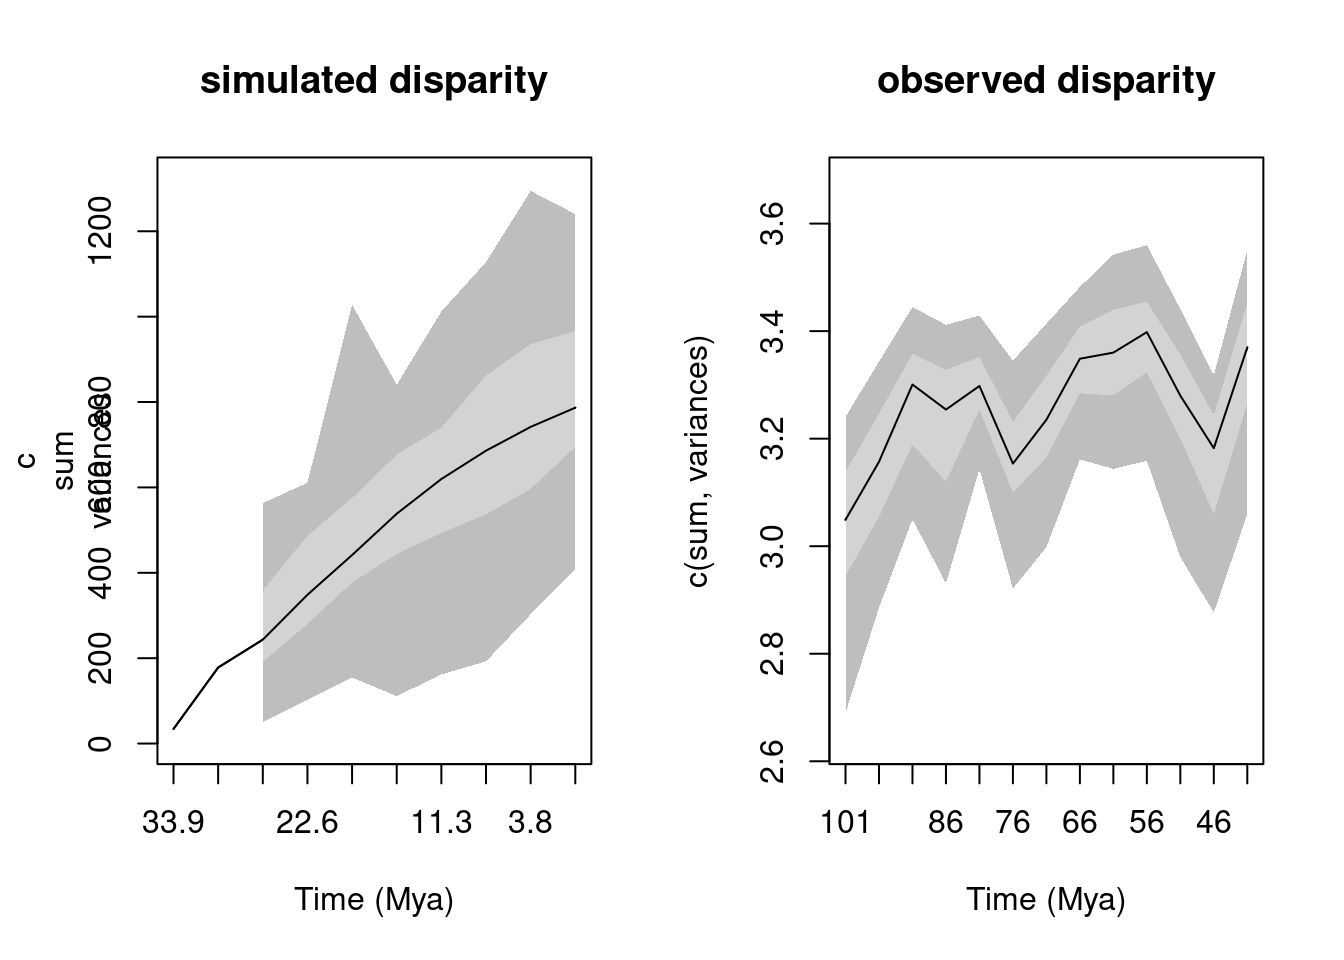
\includegraphics{treats_manual_files/figure-latex/unnamed-chunk-30-1.pdf}

We can see that both simulated and observed disparity curves are different.
From there one could already reasonably propose that the observe disparity does not entirely follows our parametrised scenario (constant speciation and extinction and BM trait evolution).

However, we can complexify our scenario to introduce the effect of mass extinction event.
We can simulate two alternative scenarios:
* one where we create a random extinction event after having simulated half of the species (25) where we remove 75\% of species;
* and a second one where we remove all the species with negative values.
This allows us to simulate two contrasted scenarios to see whether using our observed dataset it would be possible to detect changes in disparity due to mass extinctions.

To do so, we need to create two mass extinction \texttt{"event"} objects:

\begin{Shaded}
\begin{Highlighting}[]
\CommentTok{\#\# Creating a random mass extinction}
\NormalTok{random\_extinction \textless{}{-}}\StringTok{ }\KeywordTok{make.events}\NormalTok{(}\DataTypeTok{target =} \StringTok{"taxa"}\NormalTok{,}
                                 \DataTypeTok{condition =} \KeywordTok{taxa.condition}\NormalTok{(}\DecValTok{25}\NormalTok{, }\DataTypeTok{condition =} \StringTok{\textasciigrave{}}\DataTypeTok{\textgreater{}=}\StringTok{\textasciigrave{}}\NormalTok{),}
                                 \DataTypeTok{modification =} \KeywordTok{random.extinction}\NormalTok{(}\FloatTok{0.75}\NormalTok{))}
\CommentTok{\#\# Creating an extinction that removes species with negative trait values}
\NormalTok{negative\_extinction \textless{}{-}}\StringTok{ }\KeywordTok{make.events}\NormalTok{(}\DataTypeTok{target =} \StringTok{"taxa"}\NormalTok{,}
                                   \DataTypeTok{condition =} \KeywordTok{taxa.condition}\NormalTok{(}\DecValTok{25}\NormalTok{, }\DataTypeTok{condition =} \StringTok{\textasciigrave{}}\DataTypeTok{\textgreater{}=}\StringTok{\textasciigrave{}}\NormalTok{),}
                                   \DataTypeTok{modification =} \KeywordTok{trait.extinction}\NormalTok{(}\DataTypeTok{x =} \DecValTok{0}\NormalTok{, }\DataTypeTok{condition =} \StringTok{\textasciigrave{}}\DataTypeTok{\textgreater{}=}\StringTok{\textasciigrave{}}\NormalTok{))}
\end{Highlighting}
\end{Shaded}

We can then feed these two extinction events to our previous simulations

\begin{Shaded}
\begin{Highlighting}[]
\CommentTok{\#\# Simulate the tree and traits with a random extinction event}
\NormalTok{sim\_rand\_extinction \textless{}{-}}\StringTok{ }\KeywordTok{treats}\NormalTok{(}
                   \DataTypeTok{traits     =}\NormalTok{ my\_traits,}
                   \DataTypeTok{bd.params  =}\NormalTok{ est\_params,}
                   \DataTypeTok{stop.rule  =}\NormalTok{ stop\_rule,}
                   \DataTypeTok{events     =}\NormalTok{ random\_extinction,}
                   \DataTypeTok{null.error =} \DecValTok{100}\NormalTok{,}
                   \DataTypeTok{replicates =} \DecValTok{50}\NormalTok{)}

\CommentTok{\#\# Simulate the tree and traits with a random extinction event}
\NormalTok{sim\_trait\_extinction \textless{}{-}}\StringTok{ }\KeywordTok{treats}\NormalTok{(}
                   \DataTypeTok{traits     =}\NormalTok{ my\_traits,}
                   \DataTypeTok{bd.params  =}\NormalTok{ est\_params,}
                   \DataTypeTok{stop.rule  =}\NormalTok{ stop\_rule,}
                   \DataTypeTok{events     =}\NormalTok{ negative\_extinction,}
                   \DataTypeTok{null.error =} \DecValTok{100}\NormalTok{,}
                   \DataTypeTok{replicates =} \DecValTok{50}\NormalTok{)}

\CommentTok{\#\# Visualising the difference between both scenarios}
\KeywordTok{par}\NormalTok{(}\DataTypeTok{mfrow =} \KeywordTok{c}\NormalTok{(}\DecValTok{1}\NormalTok{,}\DecValTok{2}\NormalTok{))}
\KeywordTok{plot}\NormalTok{(sim\_rand\_extinction[[}\DecValTok{1}\NormalTok{]], }\DataTypeTok{main =} \StringTok{"Random extinction"}\NormalTok{)}
\KeywordTok{plot}\NormalTok{(sim\_trait\_extinction[[}\DecValTok{1}\NormalTok{]], }\DataTypeTok{main =} \StringTok{"Negative extinction"}\NormalTok{)}
\end{Highlighting}
\end{Shaded}

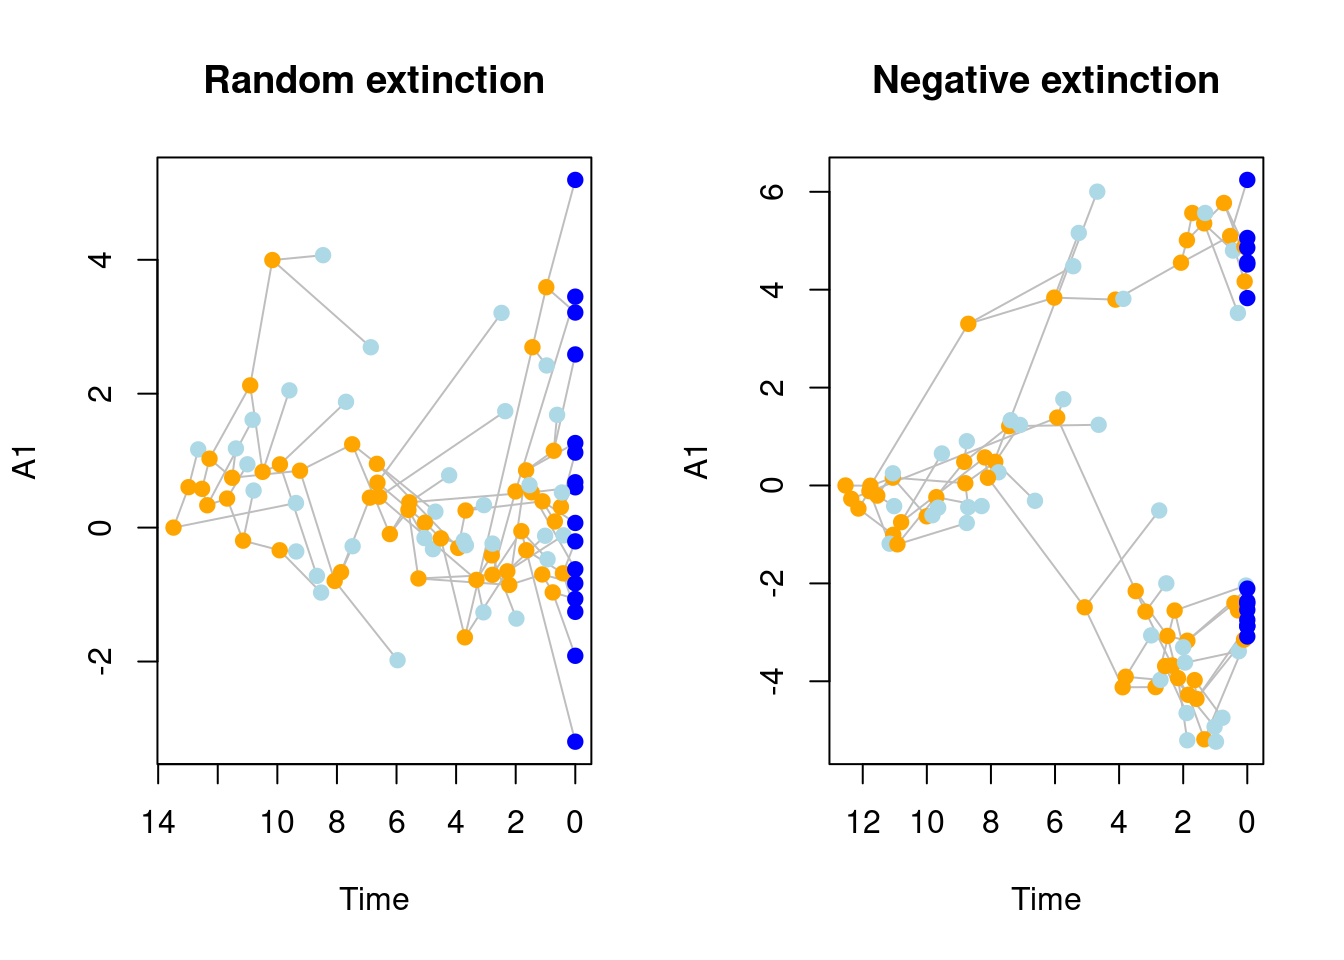
\includegraphics{treats_manual_files/figure-latex/unnamed-chunk-32-1.pdf}

We can then measure the disparity from these scenarios and compare them to our observed ones

\begin{Shaded}
\begin{Highlighting}[]
\CommentTok{\#\# Simulate the tree and traits with a random extinction event}
\NormalTok{sim\_rand\_extinction \textless{}{-}}\StringTok{ }\KeywordTok{treats}\NormalTok{(}
                   \DataTypeTok{traits     =}\NormalTok{ my\_traits,}
                   \DataTypeTok{bd.params  =}\NormalTok{ est\_params,}
                   \DataTypeTok{stop.rule  =}\NormalTok{ stop\_rule,}
                   \DataTypeTok{events     =}\NormalTok{ random\_extinction,}
                   \DataTypeTok{null.error =} \DecValTok{100}\NormalTok{,}
                   \DataTypeTok{replicates =} \DecValTok{50}\NormalTok{)}
\end{Highlighting}
\end{Shaded}

\begin{verbatim}
## Building the tree:....................Done.
## Building the tree:....Done.
## Building the tree:...........Done.
## Building the tree:.Done.
## Building the tree:............Done.
## Building the tree:.Done.
## Building the tree:.Done.
## Building the tree:.Done.
## Building the tree:..............Done.
## Building the tree:...................................Done.
## Building the tree:......................Done.
## Building the tree:........Done.
## Building the tree:...................Done.
## Building the tree:...Done.
## Building the tree:.......Done.
## Building the tree:.....Done.
## Building the tree:....................Done.
## Building the tree:.Done.
## Building the tree:...Done.
## Building the tree:................Done.
## Building the tree:.......Done.
## Building the tree:.................Done.
## Building the tree:.....Done.
## Building the tree:.................Done.
## Building the tree:............Done.
## Building the tree:....Done.
## Building the tree:....Done.
## Building the tree:...Done.
## Building the tree:...................................................Done.
## Building the tree:...............Done.
## Building the tree:....Done.
## Building the tree:.........Done.
## Building the tree:..................................Done.
## Building the tree:.....Done.
## Building the tree:........Done.
## Building the tree:....Done.
## Building the tree:.Done.
## Building the tree:...................Done.
## Building the tree:...........Done.
## Building the tree:...........Done.
## Building the tree:...........Done.
## Building the tree:.Done.
## Building the tree:...........Done.
## Building the tree:.Done.
## Building the tree:.............Done.
## Building the tree:.............Done.
## Building the tree:........Done.
## Building the tree:.............Done.
## Building the tree:...Done.
## Building the tree:.Done.
\end{verbatim}

\begin{Shaded}
\begin{Highlighting}[]
\CommentTok{\#\# Simulate the tree and traits with a random extinction event}
\NormalTok{sim\_trait\_extinction \textless{}{-}}\StringTok{ }\KeywordTok{treats}\NormalTok{(}
                   \DataTypeTok{traits     =}\NormalTok{ my\_traits,}
                   \DataTypeTok{bd.params  =}\NormalTok{ est\_params,}
                   \DataTypeTok{stop.rule  =}\NormalTok{ stop\_rule,}
                   \DataTypeTok{events     =}\NormalTok{ negative\_extinction,}
                   \DataTypeTok{null.error =} \DecValTok{100}\NormalTok{,}
                   \DataTypeTok{replicates =} \DecValTok{50}\NormalTok{)}
\end{Highlighting}
\end{Shaded}

\begin{verbatim}
## Building the tree:......................Done.
## Building the tree:...Done.
## Building the tree:..................Done.
## Building the tree:.......Done.
## Building the tree:.................Done.
## Building the tree:...Done.
## Building the tree:..................Done.
## Building the tree:....................Done.
## Building the tree:.Done.
## Building the tree:............Done.
## Building the tree:.Done.
## Building the tree:.Done.
## Building the tree:......Done.
## Building the tree:...............Done.
## Building the tree:....Done.
## Building the tree:.................Done.
## Building the tree:.........Done.
## Building the tree:....Done.
## Building the tree:.....Done.
## Building the tree:....Done.
## Building the tree:......Done.
## Building the tree:.....................Done.
## Building the tree:.................Done.
## Building the tree:.Done.
## Building the tree:....Done.
## Building the tree:...Done.
## Building the tree:...........................Done.
## Building the tree:.......Done.
## Building the tree:.......Done.
## Building the tree:.....Done.
## Building the tree:......Done.
## Building the tree:.......Done.
## Building the tree:.........Done.
## Building the tree:.....Done.
## Building the tree:...Done.
## Building the tree:...................Done.
## Building the tree:............Done.
## Building the tree:......................Done.
## Building the tree:......Done.
## Building the tree:............Done.
## Building the tree:.............Done.
## Building the tree:...........Done.
## Building the tree:..Done.
## Building the tree:.........................Done.
## Building the tree:.Done.
## Building the tree:......................Done.
## Building the tree:.............Done.
## Building the tree:...Done.
## Building the tree:...............Done.
## Building the tree:..........Done.
\end{verbatim}

\begin{Shaded}
\begin{Highlighting}[]
\CommentTok{\#\# Visualising the difference between both scenarios}
\KeywordTok{par}\NormalTok{(}\DataTypeTok{mfrow =} \KeywordTok{c}\NormalTok{(}\DecValTok{1}\NormalTok{,}\DecValTok{2}\NormalTok{))}
\KeywordTok{plot}\NormalTok{(sim\_rand\_extinction[[}\DecValTok{1}\NormalTok{]], }\DataTypeTok{main =} \StringTok{"Random extinction"}\NormalTok{)}
\KeywordTok{plot}\NormalTok{(sim\_trait\_extinction[[}\DecValTok{1}\NormalTok{]], }\DataTypeTok{main =} \StringTok{"Negative extinction"}\NormalTok{)}
\end{Highlighting}
\end{Shaded}

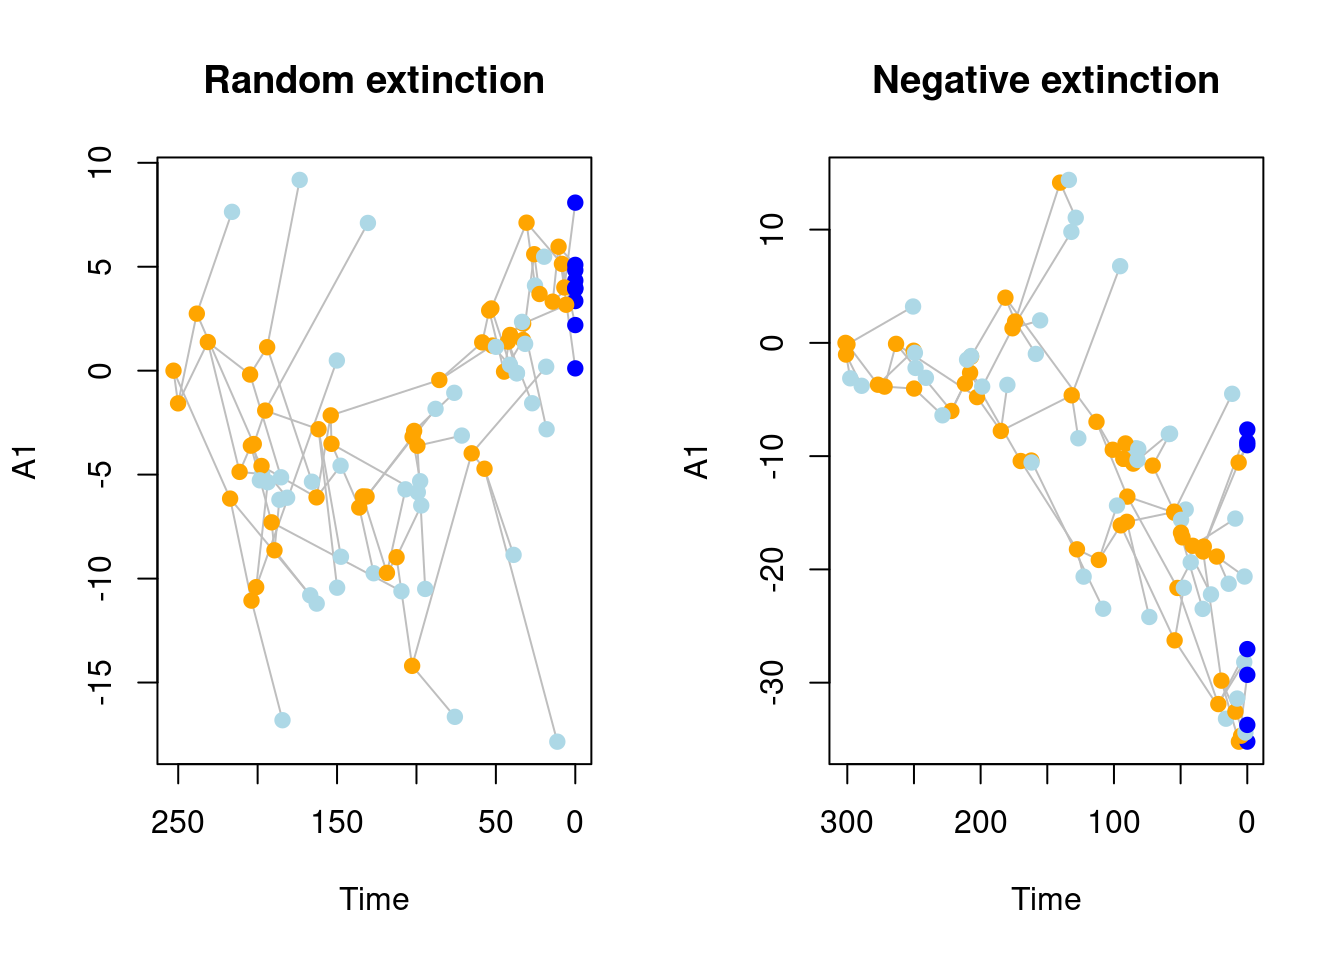
\includegraphics{treats_manual_files/figure-latex/unnamed-chunk-33-1.pdf}

Interestingly, with all our parameters used here and our specific disparity metric we cannot detect the effect of a mass extinction.

\hypertarget{maketraits}{%
\chapter{Simulating traits}\label{maketraits}}

In \texttt{treats}, traits are simulating by providing a \texttt{traits} object to the \texttt{traits} argument.
This object is generated using \texttt{make.traits}.
In \texttt{treats} a trait designate any coherent character of any number of dimensions which may or may not be independent of other traits.
For example, it can be a uni-dimensional variable uncorrelated to other traits or a multi-dimensional one with different amounts of correlation.

\begin{figure}
\centering
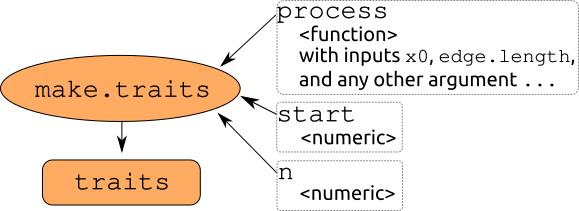
\includegraphics{make.traits.png}
\caption{\texttt{make.traits}: The main inputs are (1) the \texttt{process}, one or more functions to describe the trait(s) as a function of previous state (\texttt{x0}) and the branch length (\texttt{edge.length}), (2) \texttt{n} the number of dimensions of the trait and (3) the starting value \texttt{start}.}
\end{figure}

\hypertarget{quick-overview}{%
\subsection{Quick overview}\label{quick-overview}}

\begin{longtable}[]{@{}llll@{}}
\toprule
\begin{minipage}[b]{0.19\columnwidth}\raggedright
function\strut
\end{minipage} & \begin{minipage}[b]{0.23\columnwidth}\raggedright
arguments\strut
\end{minipage} & \begin{minipage}[b]{0.14\columnwidth}\raggedright
input\strut
\end{minipage} & \begin{minipage}[b]{0.33\columnwidth}\raggedright
what does it do\strut
\end{minipage}\tabularnewline
\midrule
\endhead
\begin{minipage}[t]{0.19\columnwidth}\raggedright
\texttt{make.traits}\strut
\end{minipage} & \begin{minipage}[t]{0.23\columnwidth}\raggedright
process*\strut
\end{minipage} & \begin{minipage}[t]{0.14\columnwidth}\raggedright
a function\strut
\end{minipage} & \begin{minipage}[t]{0.33\columnwidth}\raggedright
simulates the trait (see below)\strut
\end{minipage}\tabularnewline
\begin{minipage}[t]{0.19\columnwidth}\raggedright
\texttt{make.traits}\strut
\end{minipage} & \begin{minipage}[t]{0.23\columnwidth}\raggedright
n\strut
\end{minipage} & \begin{minipage}[t]{0.14\columnwidth}\raggedright
a numeric value\strut
\end{minipage} & \begin{minipage}[t]{0.33\columnwidth}\raggedright
the number of dimensions\strut
\end{minipage}\tabularnewline
\begin{minipage}[t]{0.19\columnwidth}\raggedright
\texttt{make.traits}\strut
\end{minipage} & \begin{minipage}[t]{0.23\columnwidth}\raggedright
start\strut
\end{minipage} & \begin{minipage}[t]{0.14\columnwidth}\raggedright
one or more numeric values\strut
\end{minipage} & \begin{minipage}[t]{0.33\columnwidth}\raggedright
the starting values for each dimensions\strut
\end{minipage}\tabularnewline
\begin{minipage}[t]{0.19\columnwidth}\raggedright
\texttt{make.traits}\strut
\end{minipage} & \begin{minipage}[t]{0.23\columnwidth}\raggedright
process.args\strut
\end{minipage} & \begin{minipage}[t]{0.14\columnwidth}\raggedright
\ldots{}\strut
\end{minipage} & \begin{minipage}[t]{0.33\columnwidth}\raggedright
anything to be passed to \texttt{process} (see below)\strut
\end{minipage}\tabularnewline
\begin{minipage}[t]{0.19\columnwidth}\raggedright
\texttt{make.traits}\strut
\end{minipage} & \begin{minipage}[t]{0.23\columnwidth}\raggedright
trait.names\strut
\end{minipage} & \begin{minipage}[t]{0.14\columnwidth}\raggedright
a character string\strut
\end{minipage} & \begin{minipage}[t]{0.33\columnwidth}\raggedright
the name(s) of the trait(s)\strut
\end{minipage}\tabularnewline
\begin{minipage}[t]{0.19\columnwidth}\raggedright
\texttt{make.traits}\strut
\end{minipage} & \begin{minipage}[t]{0.23\columnwidth}\raggedright
add\strut
\end{minipage} & \begin{minipage}[t]{0.14\columnwidth}\raggedright
a \texttt{treats} object\strut
\end{minipage} & \begin{minipage}[t]{0.33\columnwidth}\raggedright
another trait generated by \texttt{make.traits}\strut
\end{minipage}\tabularnewline
\begin{minipage}[t]{0.19\columnwidth}\raggedright
\texttt{make.traits}\strut
\end{minipage} & \begin{minipage}[t]{0.23\columnwidth}\raggedright
update\strut
\end{minipage} & \begin{minipage}[t]{0.14\columnwidth}\raggedright
a \texttt{treats} object\strut
\end{minipage} & \begin{minipage}[t]{0.33\columnwidth}\raggedright
another trait generated by \texttt{make.traits}\strut
\end{minipage}\tabularnewline
\begin{minipage}[t]{0.19\columnwidth}\raggedright
\texttt{make.traits}\strut
\end{minipage} & \begin{minipage}[t]{0.23\columnwidth}\raggedright
test\strut
\end{minipage} & \begin{minipage}[t]{0.14\columnwidth}\raggedright
logical\strut
\end{minipage} & \begin{minipage}[t]{0.33\columnwidth}\raggedright
whether to test the validity of the trait\strut
\end{minipage}\tabularnewline
\begin{minipage}[t]{0.19\columnwidth}\raggedright
\texttt{make.traits}\strut
\end{minipage} & \begin{minipage}[t]{0.23\columnwidth}\raggedright
background\strut
\end{minipage} & \begin{minipage}[t]{0.14\columnwidth}\raggedright
a \texttt{treats} object\strut
\end{minipage} & \begin{minipage}[t]{0.33\columnwidth}\raggedright
another trait generated by \texttt{make.traits} (to run in the background)\strut
\end{minipage}\tabularnewline
\begin{minipage}[t]{0.19\columnwidth}\raggedright
---------\strut
\end{minipage} & \begin{minipage}[t]{0.23\columnwidth}\raggedright
-----------\strut
\end{minipage} & \begin{minipage}[t]{0.14\columnwidth}\raggedright
-------\strut
\end{minipage} & \begin{minipage}[t]{0.33\columnwidth}\raggedright
----------------\strut
\end{minipage}\tabularnewline
\begin{minipage}[t]{0.19\columnwidth}\raggedright
\texttt{process}\strut
\end{minipage} & \begin{minipage}[t]{0.23\columnwidth}\raggedright
x0\strut
\end{minipage} & \begin{minipage}[t]{0.14\columnwidth}\raggedright
a numeric value\strut
\end{minipage} & \begin{minipage}[t]{0.33\columnwidth}\raggedright
the value of the previous trait\strut
\end{minipage}\tabularnewline
\begin{minipage}[t]{0.19\columnwidth}\raggedright
\texttt{process}\strut
\end{minipage} & \begin{minipage}[t]{0.23\columnwidth}\raggedright
edge.length\strut
\end{minipage} & \begin{minipage}[t]{0.14\columnwidth}\raggedright
a numeric value\strut
\end{minipage} & \begin{minipage}[t]{0.33\columnwidth}\raggedright
the branch length value\strut
\end{minipage}\tabularnewline
\begin{minipage}[t]{0.19\columnwidth}\raggedright
\texttt{process}\strut
\end{minipage} & \begin{minipage}[t]{0.23\columnwidth}\raggedright
\ldots{}\strut
\end{minipage} & \begin{minipage}[t]{0.14\columnwidth}\raggedright
\ldots{}\strut
\end{minipage} & \begin{minipage}[t]{0.33\columnwidth}\raggedright
any other argument to be handled by the process\strut
\end{minipage}\tabularnewline
\bottomrule
\end{longtable}

* non-optional arguments

\hypertarget{the-process-process}{%
\section{\texorpdfstring{The process (\texttt{process})}{The process (process)}}\label{the-process-process}}

The function \texttt{make.traits} allows you to design the process of a trait or a set of traits.
Here, the process of a trait designates the rules needed to generate the trait through time while simulating a phylogeny.
This process can depend on the previous state in the tree (i.e.~the trait of the ancestor) and the branch length to the descendant.
One classic example is the \href{https://en.wikipedia.org/wiki/Brownian_motion}{Brownian motion process (or Weiner process)}.
Note that it \emph{can} depend on both the ancestor and the branch length but does \emph{not necessarily need to}, i.e.~the process can be based only on the previous state or only on branch length or on neither.

\hypertarget{the-syntax-how-to-code-a-process}{%
\subsection{The syntax (how to code a process?)}\label{the-syntax-how-to-code-a-process}}

Trait processes in \texttt{treats} are functions that must always take the following arguments by default.

\begin{itemize}
\tightlist
\item
  \texttt{x0}: the previous trait value(s)
\item
  \texttt{edge.length}: the branch length
\item
  \texttt{...}: a placeholder for any extra arguments
\end{itemize}

For example, the following function would be a valid process that always generate the \emph{true} trait value: 42!.
In this example, the process is not dependent on either the previous state (\texttt{x0}) or the branch length (\texttt{edge.length}).

\begin{Shaded}
\begin{Highlighting}[]
\CommentTok{\#\# A valid (but useless?) process}
\NormalTok{valid.process \textless{}{-}}\StringTok{ }\ControlFlowTok{function}\NormalTok{(}\DataTypeTok{x0 =} \DecValTok{0}\NormalTok{, }\DataTypeTok{edge.length =} \DecValTok{1}\NormalTok{, ...) \{}
    \KeywordTok{return}\NormalTok{(}\DecValTok{42}\NormalTok{)}
\NormalTok{\}}
\end{Highlighting}
\end{Shaded}

\begin{quote}
Note that in this function definition the arguments \texttt{x0} and \texttt{edge.length} have a default value of \texttt{0} and \texttt{1} respectively. In practice, these arguments are effectively set to the correct values in the \texttt{treats} internal function (i.e.~whatever \texttt{x0} and \texttt{edge.length} are at that specific time of the process) but providing a default can help speed up the algorithms (specifically all the internal checks).
\end{quote}

On the other hand, the following process (a unidimensional Brownian motion) is incorrect (it's missing \texttt{edge.length} and \texttt{...}):

\begin{Shaded}
\begin{Highlighting}[]
\CommentTok{\#\# A wrongly formatted process}
\NormalTok{invalid.process \textless{}{-}}\StringTok{ }\ControlFlowTok{function}\NormalTok{(}\DataTypeTok{x0 =} \DecValTok{0}\NormalTok{) \{}
    \KeywordTok{return}\NormalTok{(}\KeywordTok{rnorm}\NormalTok{(}\DecValTok{1}\NormalTok{, }\DataTypeTok{mean =}\NormalTok{ x0))}
\NormalTok{\}}
\end{Highlighting}
\end{Shaded}

This will not work in \texttt{make.traits} (see below).

\hypertarget{using-a-process-in-treats}{%
\subsection{\texorpdfstring{Using a \texttt{"process"} in \texttt{treats}}{Using a "process" in treats}}\label{using-a-process-in-treats}}

You can design your own process as a function, as long as it has a valid syntax.
Alternatively, the \texttt{treats} package has several inbuilt processes, namely a multidimensional Brownian motion (\texttt{BM.process}) or a multidimensional Ornstein-Uhlenbeck process (\texttt{OU.process}).
You can find the list of implemented processes by looking at the \texttt{?trait.process} manual page in \texttt{R}.

Once a process is chosen, you can feed it into the \texttt{make.traits} function:

\begin{Shaded}
\begin{Highlighting}[]
\CommentTok{\#\# Creating a trait object}
\NormalTok{my\_trait\_object \textless{}{-}}\StringTok{ }\KeywordTok{make.traits}\NormalTok{(}\DataTypeTok{process =}\NormalTok{ BM.process)}
\end{Highlighting}
\end{Shaded}

This creates \texttt{"treats"} \texttt{"traits"} objects that you can print and visualise using the \texttt{plot} function:

\begin{Shaded}
\begin{Highlighting}[]
\CommentTok{\#\# The class of the object}
\KeywordTok{class}\NormalTok{(my\_trait\_object)}
\end{Highlighting}
\end{Shaded}

\begin{verbatim}
## [1] "treats" "traits"
\end{verbatim}

\begin{Shaded}
\begin{Highlighting}[]
\CommentTok{\#\# What\textquotesingle{}s in it?}
\NormalTok{my\_trait\_object}
\end{Highlighting}
\end{Shaded}

\begin{verbatim}
##  ---- treats traits object ---- 
## 1 trait for 1 process (A) with one starting value (0).
\end{verbatim}

\begin{Shaded}
\begin{Highlighting}[]
\CommentTok{\#\# What does the process looks like}
\KeywordTok{plot}\NormalTok{(my\_trait\_object)}
\end{Highlighting}
\end{Shaded}

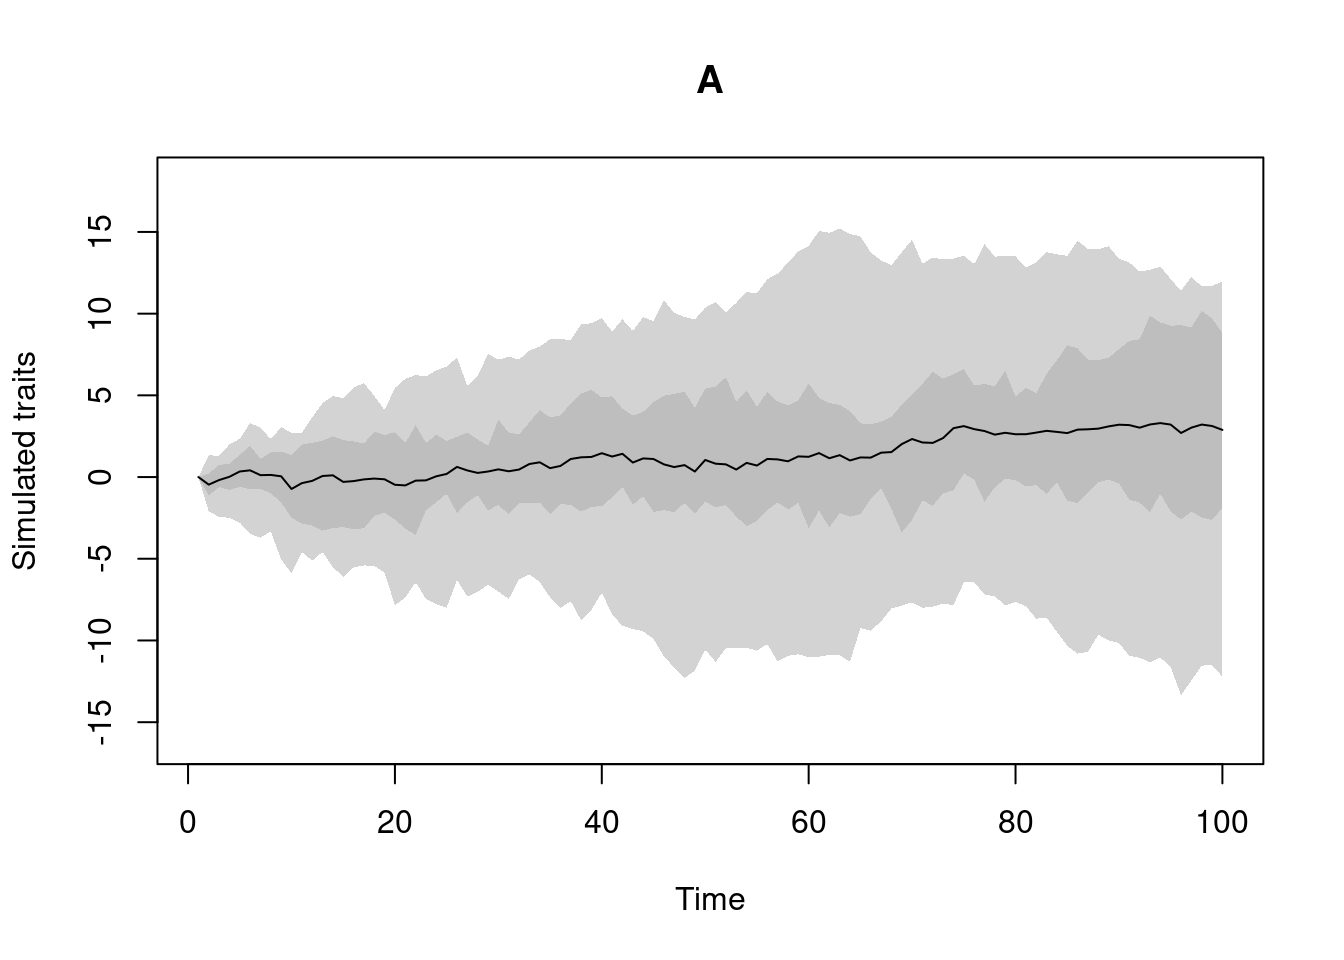
\includegraphics{treats_manual_files/figure-latex/unnamed-chunk-38-1.pdf}

Note that you can see the multiple options for plotting the trait process by looking at \texttt{?plot.treats} manual. Furthermore, you can look at what's actually in the object using this specific syntax (this applies to every object handled by the \texttt{treats} package):

\begin{Shaded}
\begin{Highlighting}[]
\CommentTok{\#\# What\textquotesingle{}s actually in that object?}
\KeywordTok{print.treats}\NormalTok{(my\_trait\_object, }\DataTypeTok{all =} \OtherTok{TRUE}\NormalTok{)}
\end{Highlighting}
\end{Shaded}

\begin{verbatim}
## $main
## $main$A
## $main$A$process
## function (x0 = 0, edge.length = 1, Sigma = diag(length(x0)), 
##     ...) 
## {
##     return(t(MASS::mvrnorm(n = 1, mu = x0, Sigma = Sigma * edge.length, 
##         ...)))
## }
## <bytecode: 0x609b29299e58>
## <environment: namespace:treats>
## 
## $main$A$start
## [1] 0
## 
## $main$A$trait_id
## [1] 1
## 
## 
## 
## $background
## NULL
\end{verbatim}

As traits can get more and more complex, the automatic printing of its summary allows for a easier display of what's in the \texttt{"traits"} object.

Note that it is possible to make \texttt{"traits"} objects with multiple traits and multiple processes (that can be the same or different for each trait):

\begin{Shaded}
\begin{Highlighting}[]
\CommentTok{\#\# Four traits: two BM, one OU and one normal non process}
\NormalTok{four\_traits \textless{}{-}}\StringTok{ }\KeywordTok{make.traits}\NormalTok{(}\DataTypeTok{process =} \KeywordTok{c}\NormalTok{(BM.process,}
\NormalTok{                                       BM.process,}
\NormalTok{                                       OU.process,}
\NormalTok{                                       no.process))}
\NormalTok{four\_traits}
\end{Highlighting}
\end{Shaded}

\begin{verbatim}
##  ---- treats traits object ---- 
## 4 traits for 4 processes (A, B, C, D) with one starting value (0).
\end{verbatim}

You can visualise them individually using the \texttt{trait} argument in \texttt{plot.treats}:

\begin{Shaded}
\begin{Highlighting}[]
\CommentTok{\#\# Plot options (4 plots in one window)}
\KeywordTok{par}\NormalTok{(}\DataTypeTok{mfrow =} \KeywordTok{c}\NormalTok{(}\DecValTok{2}\NormalTok{,}\DecValTok{2}\NormalTok{))}
\KeywordTok{plot}\NormalTok{(four\_traits, }\DataTypeTok{trait =} \DecValTok{1}\NormalTok{)}
\KeywordTok{plot}\NormalTok{(four\_traits, }\DataTypeTok{trait =} \DecValTok{2}\NormalTok{)}
\KeywordTok{plot}\NormalTok{(four\_traits, }\DataTypeTok{trait =} \DecValTok{3}\NormalTok{)}
\KeywordTok{plot}\NormalTok{(four\_traits, }\DataTypeTok{trait =} \DecValTok{4}\NormalTok{)}
\end{Highlighting}
\end{Shaded}

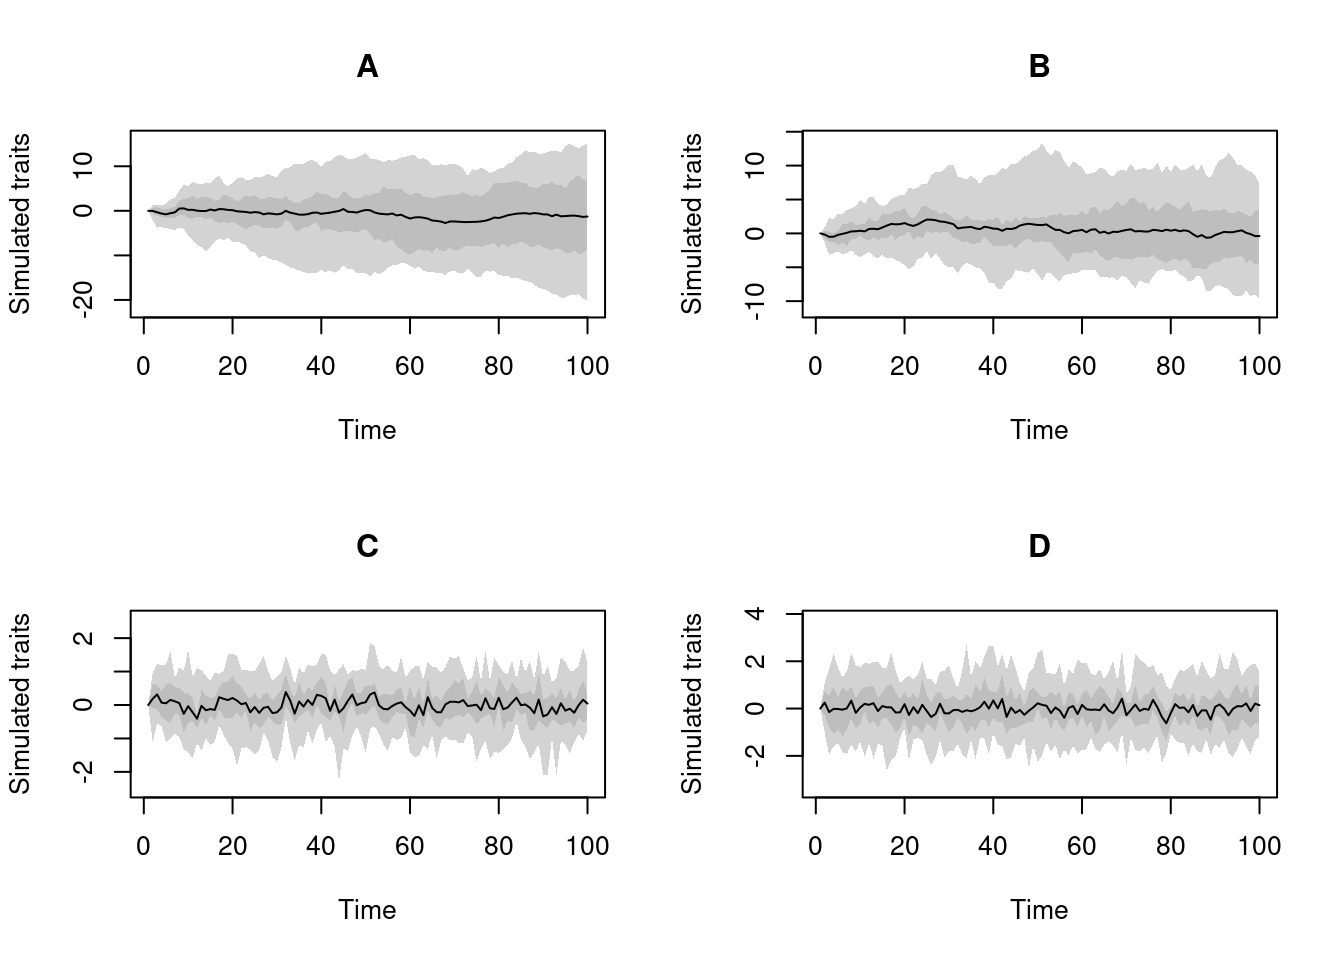
\includegraphics{treats_manual_files/figure-latex/unnamed-chunk-41-1.pdf}

\begin{Shaded}
\begin{Highlighting}[]
\KeywordTok{par}\NormalTok{(}\DataTypeTok{mfrow =} \KeywordTok{c}\NormalTok{(}\DecValTok{1}\NormalTok{,}\DecValTok{1}\NormalTok{))}
\end{Highlighting}
\end{Shaded}

\hypertarget{the-number-of-traits-n-and-the-starting-values-start}{%
\section{\texorpdfstring{The number of traits \texttt{n} and the starting values \texttt{start}}{The number of traits n and the starting values start}}\label{the-number-of-traits-n-and-the-starting-values-start}}

Two further important arguments are \texttt{n} the number of traits per process and \texttt{start} the starting values for all traits.
By default they are set to \texttt{n\ =\ 1} and \texttt{start\ =\ 0}.
This means that \texttt{make.traits} will assume that your processes are always unidimensional by default and that they always start with the value \texttt{0}.
It is possible however, to change these values.

For example you can use the following to create a three dimensional Brownian motion with each dimension starting with the value \texttt{1}:

\begin{Shaded}
\begin{Highlighting}[]
\CommentTok{\#\# Multidimensional Brownian motion}
\KeywordTok{make.traits}\NormalTok{(BM.process, }\DataTypeTok{n =} \DecValTok{3}\NormalTok{, }\DataTypeTok{start =} \DecValTok{1}\NormalTok{)}
\end{Highlighting}
\end{Shaded}

\begin{verbatim}
##  ---- treats traits object ---- 
## 3 traits for 1 process (A:3) with one starting value (1).
\end{verbatim}

Or the following with each dimensions starting with different values (respectively \texttt{1}, \texttt{2} and \texttt{3}):

\begin{Shaded}
\begin{Highlighting}[]
\CommentTok{\#\# Multidimensional Brownian motion}
\KeywordTok{make.traits}\NormalTok{(BM.process, }\DataTypeTok{n =} \DecValTok{3}\NormalTok{, }\DataTypeTok{start =} \KeywordTok{c}\NormalTok{(}\DecValTok{1}\NormalTok{,}\DecValTok{2}\NormalTok{,}\DecValTok{3}\NormalTok{))}
\end{Highlighting}
\end{Shaded}

\begin{verbatim}
##  ---- treats traits object ---- 
## 3 traits for 1 process (A:3) with different starting values (1,2,3).
\end{verbatim}

Note that the number of traits are applied for each process by default.
However, you can apply different number of traits for different processes:

\begin{Shaded}
\begin{Highlighting}[]
\CommentTok{\#\# two 3D processes (BM and OU)}
\KeywordTok{make.traits}\NormalTok{(}\KeywordTok{c}\NormalTok{(BM.process, OU.process), }\DataTypeTok{n =} \DecValTok{3}\NormalTok{)}
\end{Highlighting}
\end{Shaded}

\begin{verbatim}
##  ---- treats traits object ---- 
## 6 traits for 2 processes (A:3, B:3) with one starting value (0).
\end{verbatim}

\begin{Shaded}
\begin{Highlighting}[]
\CommentTok{\#\# one 1D processes (BM) and one 4D process (OU)}
\KeywordTok{make.traits}\NormalTok{(}\KeywordTok{c}\NormalTok{(BM.process, OU.process), }\DataTypeTok{n =} \KeywordTok{c}\NormalTok{(}\DecValTok{1}\NormalTok{, }\DecValTok{4}\NormalTok{))}
\end{Highlighting}
\end{Shaded}

\begin{verbatim}
##  ---- treats traits object ---- 
## 5 traits for 2 processes (A:1, B:4) with one starting value (0).
\end{verbatim}

And starting values are distributed for all the traits or for the traits one by one:

\begin{Shaded}
\begin{Highlighting}[]
\CommentTok{\#\# two 3D processes (BM and OU) starting with 1}
\KeywordTok{make.traits}\NormalTok{(}\KeywordTok{c}\NormalTok{(BM.process, OU.process), }\DataTypeTok{n =} \DecValTok{3}\NormalTok{, }\DataTypeTok{start =} \DecValTok{1}\NormalTok{)}
\end{Highlighting}
\end{Shaded}

\begin{verbatim}
##  ---- treats traits object ---- 
## 6 traits for 2 processes (A:3, B:3) with one starting value (1).
\end{verbatim}

\begin{Shaded}
\begin{Highlighting}[]
\CommentTok{\#\# two 3D processes (BM and OU) starting with values 1 to 6}
\KeywordTok{make.traits}\NormalTok{(}\KeywordTok{c}\NormalTok{(BM.process, OU.process), }\DataTypeTok{n =} \DecValTok{3}\NormalTok{, }\DataTypeTok{start =} \DecValTok{1}\OperatorTok{:}\DecValTok{6}\NormalTok{)}
\end{Highlighting}
\end{Shaded}

\begin{verbatim}
##  ---- treats traits object ---- 
## 6 traits for 2 processes (A:3, B:3) with different starting values (1,2,3,4,5,6).
\end{verbatim}

\begin{Shaded}
\begin{Highlighting}[]
\CommentTok{\#\# two 3D processes (BM and OU) with the two first ones starting}
\CommentTok{\#\# with 1 and the 4 other ones with the default (0)}
\KeywordTok{make.traits}\NormalTok{(}\KeywordTok{c}\NormalTok{(BM.process, OU.process), }\DataTypeTok{n =} \DecValTok{3}\NormalTok{, }\DataTypeTok{start =} \KeywordTok{c}\NormalTok{(}\DecValTok{1}\NormalTok{,}\DecValTok{1}\NormalTok{))}
\end{Highlighting}
\end{Shaded}

\begin{verbatim}
## Warning in make.traits(c(BM.process, OU.process), n = 3, start = c(1, 1)): Only
## the first 2 starting values were supplied for a required 6 traits. The missing
## start values are set to 0.
\end{verbatim}

\begin{verbatim}
##  ---- treats traits object ---- 
## 6 traits for 2 processes (A:3, B:3) with different starting values (1,1,0,0,0,0).
\end{verbatim}

\hypertarget{what-is-a-trait-in-treats}{%
\subsection{\texorpdfstring{What is a trait in \texttt{treats}?}{What is a trait in treats?}}\label{what-is-a-trait-in-treats}}

Because it would be impossible to accommodate all definitions of a trait in \texttt{treats} we chose an arbitrary one: a trait is whatever you define as a trait!
A trait can be uni-dimensional as the measurement of a feature of an organism (e.g.~leaf surface, femur length, etc.) but can also be a multi-dimensional description of a feature, for example in 3D geometric morphometric context, a trait could be defined as ``position of landmark X'' (which will be a trait with three dimensions, \emph{x}, \emph{y} and \emph{z}) or in ecology, the location of a plant can be expressed as latitude and longitude coordinates.
In \texttt{treats}, the \textbf{process} corresponds to this trait definition (e.g.~a process can be of n-dimensions and represents one organisms feature) and the \textbf{traits} represents the number of dimensions in total.
So in the examples above, this is how the following traits are interpreted by \texttt{treats}:

\begin{Shaded}
\begin{Highlighting}[]
\CommentTok{\#\# Three traits with one process:}
\KeywordTok{make.traits}\NormalTok{(BM.process, }\DataTypeTok{n =} \DecValTok{3}\NormalTok{, }\DataTypeTok{start =} \KeywordTok{c}\NormalTok{(}\DecValTok{1}\NormalTok{,}\DecValTok{2}\NormalTok{,}\DecValTok{3}\NormalTok{))}
\CommentTok{\#\# Six traits with two processes:}
\KeywordTok{make.traits}\NormalTok{(}\KeywordTok{c}\NormalTok{(BM.process, OU.process), }\DataTypeTok{n =} \DecValTok{3}\NormalTok{)}
\CommentTok{\#\# Five traits with two processes}
\KeywordTok{make.traits}\NormalTok{(}\KeywordTok{c}\NormalTok{(BM.process, OU.process), }\DataTypeTok{n =} \KeywordTok{c}\NormalTok{(}\DecValTok{1}\NormalTok{, }\DecValTok{4}\NormalTok{))}
\end{Highlighting}
\end{Shaded}

\hypertarget{multidimensional-traits-and-correlations}{%
\section{Multidimensional traits and correlations}\label{multidimensional-traits-and-correlations}}

As shown in the example above, a trait can be made multidimensional by using the \texttt{n} argument specifically passed to a \texttt{process}.
However, in this case, traits are simulated independently of each other.
It is possible to include correlation by designing a multidimensional trait \texttt{process} directly generating the correlation between within the dimensions of the process.
Alternatively, the inbuilt \texttt{BM.process} and \texttt{OU.process} can intake a correlation matrix to simulate traits independtly but with a correlation coefficient (see \protect\hyperlink{EG_change_correlation}{this illustration with an event}).

\hypertarget{extra-argument-for-the-processes-with-process.args}{%
\section{\texorpdfstring{Extra argument for the processes with \texttt{process.args}}{Extra argument for the processes with process.args}}\label{extra-argument-for-the-processes-with-process.args}}

You can also feed extra arguments to your process(es) functions.
For example, the inbuilt process \texttt{no.process} (that is just a number generator not based on the previous value \texttt{x0} or the branch length) can take a specific random number generator as a function:

\begin{Shaded}
\begin{Highlighting}[]
\CommentTok{\#\# no process trait using the normal distribution (default)}
\KeywordTok{make.traits}\NormalTok{(no.process, }\DataTypeTok{process.args =} \KeywordTok{list}\NormalTok{(}\DataTypeTok{fun =}\NormalTok{ rnorm))}
\end{Highlighting}
\end{Shaded}

\begin{verbatim}
##  ---- treats traits object ---- 
## 1 trait for 1 process (A) with one starting value (0).
## process A uses the following extra argument: fun;
\end{verbatim}

\begin{Shaded}
\begin{Highlighting}[]
\CommentTok{\#\# no process trait using the uniform distribution}
\CommentTok{\#\# bounded between 1 and 100}
\KeywordTok{make.traits}\NormalTok{(no.process, }\DataTypeTok{process.args =} \KeywordTok{list}\NormalTok{(}\DataTypeTok{fun =}\NormalTok{ runif, }\DataTypeTok{min =} \DecValTok{1}\NormalTok{, }\DataTypeTok{max =} \DecValTok{100}\NormalTok{))}
\end{Highlighting}
\end{Shaded}

\begin{verbatim}
##  ---- treats traits object ---- 
## 1 trait for 1 process (A) with one starting value (0).
## process A uses the following extra arguments: fun,min,max;
\end{verbatim}

You can also add multiple extra arguments for multiple processes giving them as a list.

\begin{Shaded}
\begin{Highlighting}[]
\CommentTok{\#\# Two traits with no process:one normal and one uniform (1,100)}
\KeywordTok{make.traits}\NormalTok{(}\DataTypeTok{process =} \KeywordTok{c}\NormalTok{(no.process, no.process),}
            \DataTypeTok{process.args =} \KeywordTok{list}\NormalTok{(}\KeywordTok{list}\NormalTok{(}\DataTypeTok{fun =}\NormalTok{ rnorm),}
                                \KeywordTok{list}\NormalTok{(}\DataTypeTok{fun =}\NormalTok{ runif, }\DataTypeTok{min =} \DecValTok{1}\NormalTok{, }\DataTypeTok{max =} \DecValTok{100}\NormalTok{)))}
\end{Highlighting}
\end{Shaded}

\begin{verbatim}
##  ---- treats traits object ---- 
## 2 traits for 2 processes (A, B) with one starting value (0).
## process A uses the following extra argument: fun;
## process B uses the following extra arguments: fun,min,max;
\end{verbatim}

If one process does not need extra argument you must still give it an extra \texttt{NULL} process argument:

\begin{Shaded}
\begin{Highlighting}[]
\CommentTok{\#\# Three traits with no process:}
\CommentTok{\#\# one default, one lognormal and one uniform (1,100)}
\KeywordTok{make.traits}\NormalTok{(}\DataTypeTok{process      =} \KeywordTok{c}\NormalTok{(no.process, no.process, no.process),}
            \DataTypeTok{process.args =} \KeywordTok{list}\NormalTok{(}\CommentTok{\#\# Extra arguments for the first process (none)}
                                \KeywordTok{list}\NormalTok{(}\OtherTok{NULL}\NormalTok{),}
                                \CommentTok{\#\# Extra arguments for the second process}
                                \KeywordTok{list}\NormalTok{(}\DataTypeTok{fun =}\NormalTok{ rlnorm),}
                                \CommentTok{\#\# Extra arguments for the third process}
                                \KeywordTok{list}\NormalTok{(}\DataTypeTok{fun =}\NormalTok{ runif, }\DataTypeTok{min =} \DecValTok{1}\NormalTok{, }\DataTypeTok{max =} \DecValTok{100}\NormalTok{)))}
\end{Highlighting}
\end{Shaded}

\begin{verbatim}
##  ---- treats traits object ---- 
## 3 traits for 3 processes (A, B, C) with one starting value (0).
## process B uses the following extra argument: fun;
## process C uses the following extra arguments: fun,min,max;
\end{verbatim}

\hypertarget{naming-the-traits-with-trait.names}{%
\section{\texorpdfstring{Naming the traits with \texttt{trait.names}}{Naming the traits with trait.names}}\label{naming-the-traits-with-trait.names}}

As traits become more and more complex, it can be useful to give clearer names to each process.
This is easily done using the \texttt{trait.names} argument that attributes one name per process:

\begin{Shaded}
\begin{Highlighting}[]
\CommentTok{\#\# A simple trait with a proper name}
\NormalTok{simple\_trait \textless{}{-}}\StringTok{ }\KeywordTok{make.traits}\NormalTok{(}\DataTypeTok{trait.names =} \StringTok{"1D Brownian Motion"}\NormalTok{)}
\NormalTok{simple\_trait}
\end{Highlighting}
\end{Shaded}

\begin{verbatim}
##  ---- treats traits object ---- 
## 1 trait for 1 process (1D Brownian Motion) with one starting value (0).
\end{verbatim}

This becomes more useful if we use the complex example above:

\begin{Shaded}
\begin{Highlighting}[]
\CommentTok{\#\# Three named traits with no process:}
\CommentTok{\#\# one default, one lognormal and one uniform (1,100)}
\KeywordTok{make.traits}\NormalTok{(}\DataTypeTok{process      =} \KeywordTok{c}\NormalTok{(no.process, no.process, no.process),}
            \DataTypeTok{process.args =} \KeywordTok{list}\NormalTok{(}\CommentTok{\#\# Extra arguments for the first process (none)}
                                \KeywordTok{list}\NormalTok{(}\OtherTok{NULL}\NormalTok{),}
                                \CommentTok{\#\# Extra arguments for the second process}
                                \KeywordTok{list}\NormalTok{(}\DataTypeTok{fun =}\NormalTok{ rlnorm),}
                                \CommentTok{\#\# Extra arguments for the third process}
                                \KeywordTok{list}\NormalTok{(}\DataTypeTok{fun =}\NormalTok{ runif, }\DataTypeTok{min =} \DecValTok{1}\NormalTok{, }\DataTypeTok{max =} \DecValTok{100}\NormalTok{)),}
            \CommentTok{\#\# Naming each trait}
            \DataTypeTok{trait.names  =} \KeywordTok{c}\NormalTok{(}\StringTok{"Normal"}\NormalTok{, }\StringTok{"LogNormal"}\NormalTok{, }\StringTok{"Uniform(1,100)"}\NormalTok{))}
\end{Highlighting}
\end{Shaded}

\begin{verbatim}
##  ---- treats traits object ---- 
## 3 traits for 3 processes (Normal, LogNormal, Uniform(1,100)) with one starting value (0).
## process LogNormal uses the following extra argument: fun;
## process Uniform(1,100) uses the following extra arguments: fun,min,max;
\end{verbatim}

\hypertarget{combining-multiple-traits-with-add}{%
\section{\texorpdfstring{Combining multiple traits with \texttt{add}}{Combining multiple traits with add}}\label{combining-multiple-traits-with-add}}

You can also add traits to already existing trait objects using the simple \texttt{add} option.
This option just takes a \texttt{"treats"} \texttt{"traits"} object and the additional process(es) will be added to it.
For example:

\begin{Shaded}
\begin{Highlighting}[]
\CommentTok{\#\# Creating a simple default Brownian motion}
\NormalTok{one\_process \textless{}{-}}\StringTok{ }\KeywordTok{make.traits}\NormalTok{(}\DataTypeTok{trait.names =} \StringTok{"BM"}\NormalTok{)}

\CommentTok{\#\# Creating a new trait (a 3D OU.process)}
\CommentTok{\#\# and adding the previous one}
\NormalTok{two\_processes \textless{}{-}}\StringTok{ }\KeywordTok{make.traits}\NormalTok{(OU.process, }\DataTypeTok{n =} \DecValTok{3}\NormalTok{, }\DataTypeTok{add =}\NormalTok{ one\_process,}
                             \DataTypeTok{trait.names =} \StringTok{"3D OU"}\NormalTok{)}

\CommentTok{\#\# Only one process}
\NormalTok{one\_process}
\end{Highlighting}
\end{Shaded}

\begin{verbatim}
##  ---- treats traits object ---- 
## 1 trait for 1 process (BM) with one starting value (0).
\end{verbatim}

\begin{Shaded}
\begin{Highlighting}[]
\CommentTok{\#\# The two processes}
\NormalTok{two\_processes}
\end{Highlighting}
\end{Shaded}

\begin{verbatim}
##  ---- treats traits object ---- 
## 4 traits for 2 processes (BM:1, 3D OU:3) with one starting value (0).
\end{verbatim}

\hypertarget{using-a-background-trait}{%
\section{Using a background trait}\label{using-a-background-trait}}

\texttt{traits} objects also allow a background trait to be used when traits are simulated (\protect\hyperlink{bdalgorithm}{step 3 here}).
This allows traits to be simulated for \emph{all} tips whenever a trait is generated for one tip.
This can be useful for keeping track of trait values along the simulation (\emph{cf} just at bifurcating nodes).
The \texttt{background} argument takes any output from the \texttt{make.traits} function in a nested way:

\begin{Shaded}
\begin{Highlighting}[]
\CommentTok{\#\# Generating a default BM trait:}
\NormalTok{BM\_trait \textless{}{-}}\StringTok{ }\KeywordTok{make.traits}\NormalTok{()}
\CommentTok{\#\# Generating an OU trait with a background BM trait}
\NormalTok{my\_trait \textless{}{-}}\StringTok{ }\KeywordTok{make.traits}\NormalTok{(}\DataTypeTok{process =}\NormalTok{ OU.process, }\DataTypeTok{background =}\NormalTok{ BM\_trait) }
\end{Highlighting}
\end{Shaded}

Note that technically you can nest as many background traits as you want (e.g.~\texttt{make.traits(background\ =\ make.traits(background\ =\ make.traits(...)))} is valid).
However, you should always make sure that the background trait has the same dimensions as the main trait.
When using a trait with background, your tree will have internal singleton nodes (i.e.~nodes linking to one ancestor and only one descendant).
You can remove these nodes using the \protect\hyperlink{dropthings}{\texttt{drop.things} function}.

\begin{Shaded}
\begin{Highlighting}[]
\KeywordTok{set.seed}\NormalTok{(}\DecValTok{1}\NormalTok{)}
\CommentTok{\#\# Generating a pure birth tree with the background trait}
\NormalTok{tree\_bkg \textless{}{-}}\StringTok{ }\KeywordTok{treats}\NormalTok{(}\DataTypeTok{stop.rule =} \KeywordTok{list}\NormalTok{(}\DataTypeTok{max.taxa =} \DecValTok{20}\NormalTok{),}
                 \DataTypeTok{traits =}\NormalTok{ my\_trait)}
\CommentTok{\#\# This tree has many internal singleton nodes}
\KeywordTok{plot}\NormalTok{(tree\_bkg)}
\end{Highlighting}
\end{Shaded}

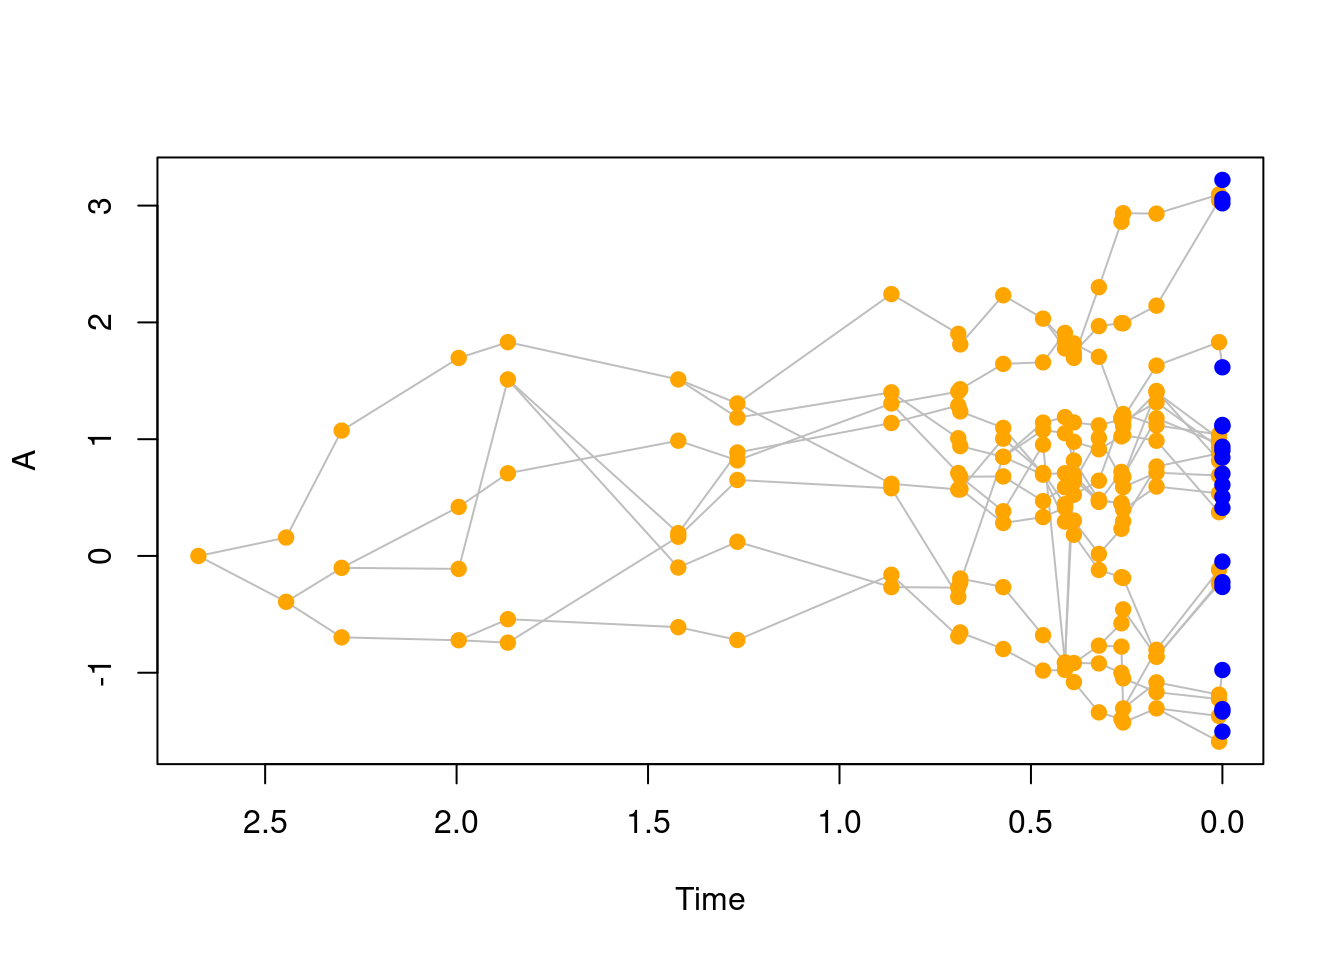
\includegraphics{treats_manual_files/figure-latex/unnamed-chunk-54-1.pdf}

\hypertarget{saving-trait-values-at-different-time-steps}{%
\section{Saving trait values at different time steps}\label{saving-trait-values-at-different-time-steps}}

You can also simulate a tree by generating traits at specific time steps with the \texttt{save.steps} option in \texttt{treats}.
This will apply the \texttt{traits} object to all lineages currently alive at the required time steps.
These time steps can be either regular by providing a single numeric value; e.g.~\texttt{save.steps\ =\ 0.1} will take a snapshot of the trait values every 0.1 units of time, or specific, by providing a specific set of values; e.g.~\texttt{save.steps\ =\ c(1,\ 1.2,\ 3)} will take a snapshot of the trait values at the required time steps.

\begin{Shaded}
\begin{Highlighting}[]
\KeywordTok{set.seed}\NormalTok{(}\DecValTok{123}\NormalTok{)}
\CommentTok{\#\# Generating a birth{-}death tree with a BM trait and saving steps at specific times}
\NormalTok{tree\_steps \textless{}{-}}\StringTok{ }\KeywordTok{treats}\NormalTok{(}\DataTypeTok{stop.rule  =} \KeywordTok{list}\NormalTok{(}\DataTypeTok{max.time =} \DecValTok{3}\NormalTok{),}
                   \DataTypeTok{bd.params  =} \KeywordTok{list}\NormalTok{(}\DataTypeTok{speciation =} \DecValTok{1}\NormalTok{, }\DataTypeTok{extinction =} \FloatTok{0.1}\NormalTok{),}
                   \DataTypeTok{traits     =} \KeywordTok{make.traits}\NormalTok{(),}
                   \DataTypeTok{save.steps =} \KeywordTok{c}\NormalTok{(}\DecValTok{1}\OperatorTok{/}\DecValTok{3}\NormalTok{, }\DecValTok{1}\NormalTok{, }\DecValTok{2}\NormalTok{))}
\CommentTok{\#\# This also creates internal singleton nodes}
\KeywordTok{plot}\NormalTok{(tree\_steps)}
\KeywordTok{abline}\NormalTok{(}\DataTypeTok{v =} \DecValTok{3} \OperatorTok{{-}}\StringTok{ }\KeywordTok{c}\NormalTok{(}\DecValTok{1}\OperatorTok{/}\DecValTok{3}\NormalTok{, }\DecValTok{1}\NormalTok{, }\DecValTok{2}\NormalTok{), }\DataTypeTok{lwd =} \FloatTok{0.5}\NormalTok{, }\DataTypeTok{col =} \StringTok{"grey"}\NormalTok{)}
\end{Highlighting}
\end{Shaded}

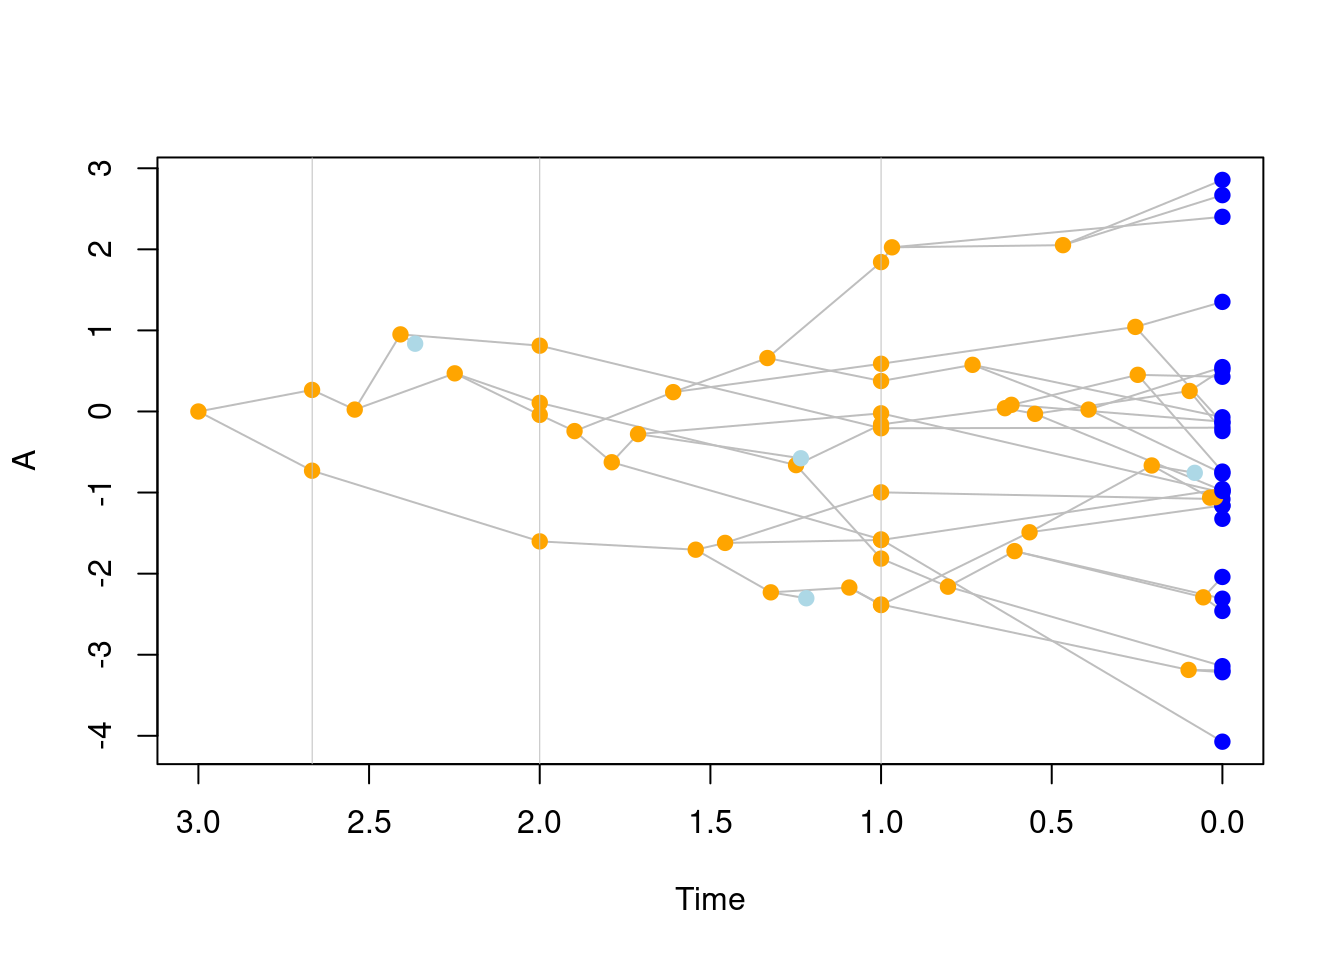
\includegraphics{treats_manual_files/figure-latex/unnamed-chunk-55-1.pdf}

\hypertarget{traits-implemented-in-treats}{%
\section{\texorpdfstring{Traits implemented in \texttt{treats}}{Traits implemented in treats}}\label{traits-implemented-in-treats}}

If you don't want to design your own trait process, you can use one of the following trait processes that are currently implemented in \texttt{treats}. You can find more information about their many options using their specific manuals in R or the generic \texttt{?trait.process}:

\begin{itemize}
\tightlist
\item
  \texttt{BM.process}: this is the well known \href{https://en.wikipedia.org/wiki/Brownian_motion}{Brownian motion process}.
\end{itemize}

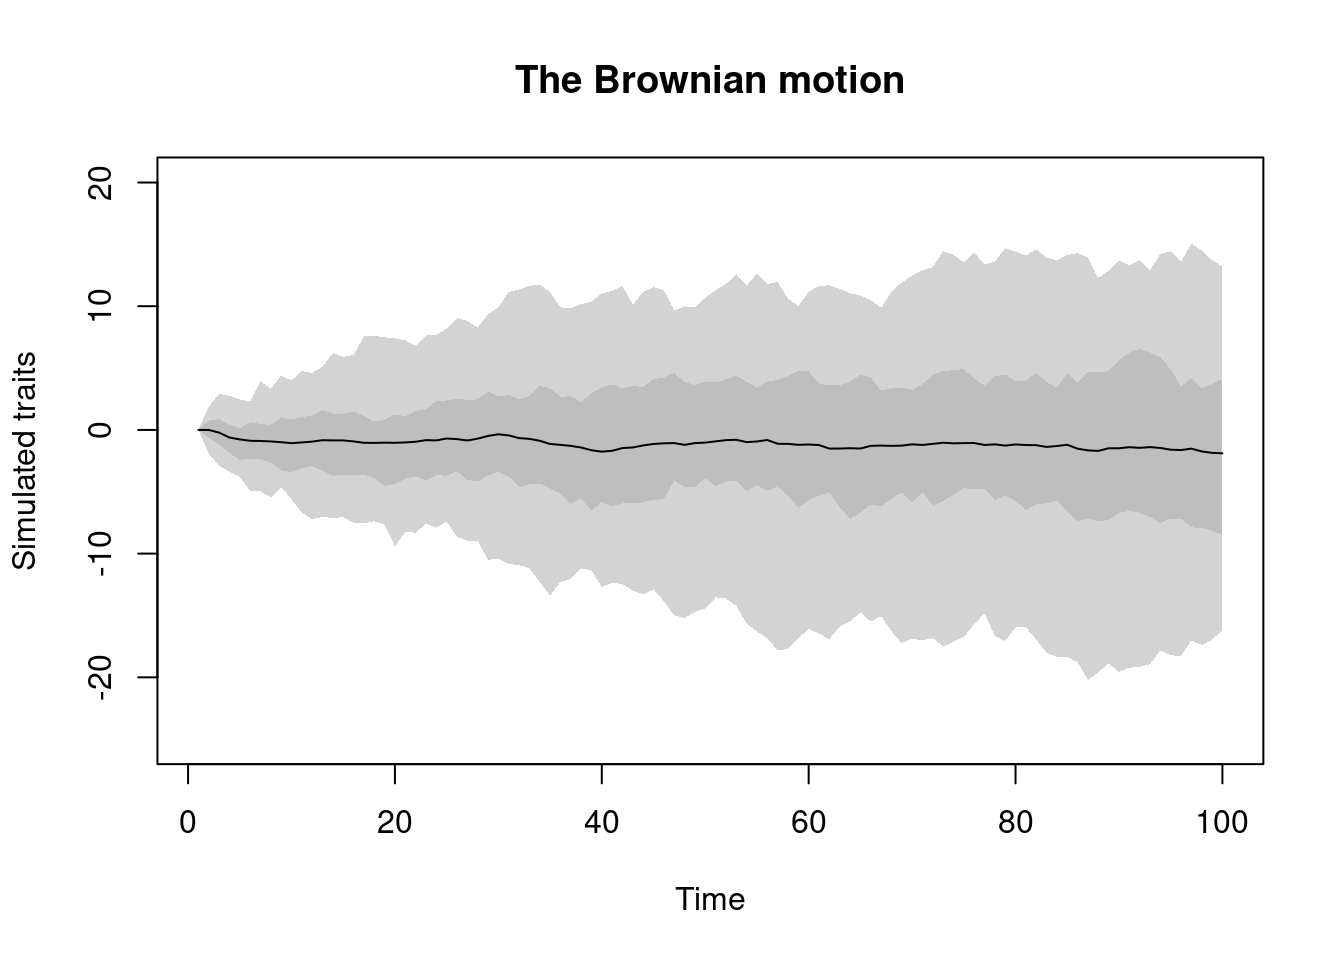
\includegraphics{treats_manual_files/figure-latex/unnamed-chunk-56-1.pdf}

\begin{itemize}
\tightlist
\item
  \texttt{OU.process}: this is the equally famous \href{https://en.wikipedia.org/wiki/Ornstein\%E2\%80\%93Uhlenbeck_process}{Ornstein--Uhlenbeck process}.
\end{itemize}

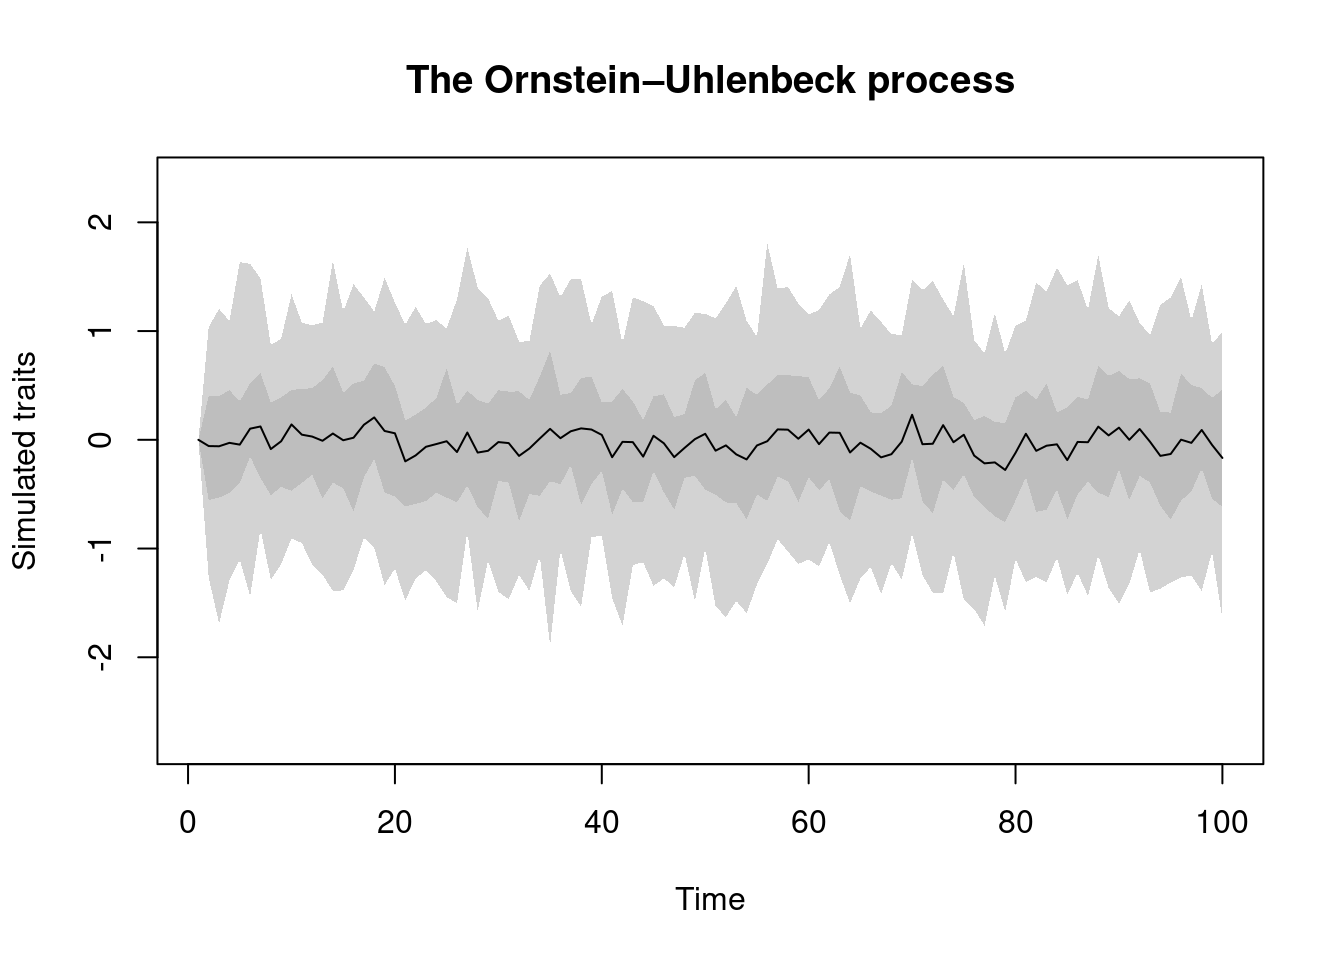
\includegraphics{treats_manual_files/figure-latex/unnamed-chunk-57-1.pdf}

\begin{itemize}
\tightlist
\item
  \texttt{no.process}: this process has\ldots{} no process. In other words, this is a non time dependent process; the simulated value does not depends on the ancestors' value nor the branch length. It's basically a place holder for a random sampling function like \texttt{rnorm} (default), \texttt{runif}, \texttt{rlnorm}, etc.
\end{itemize}

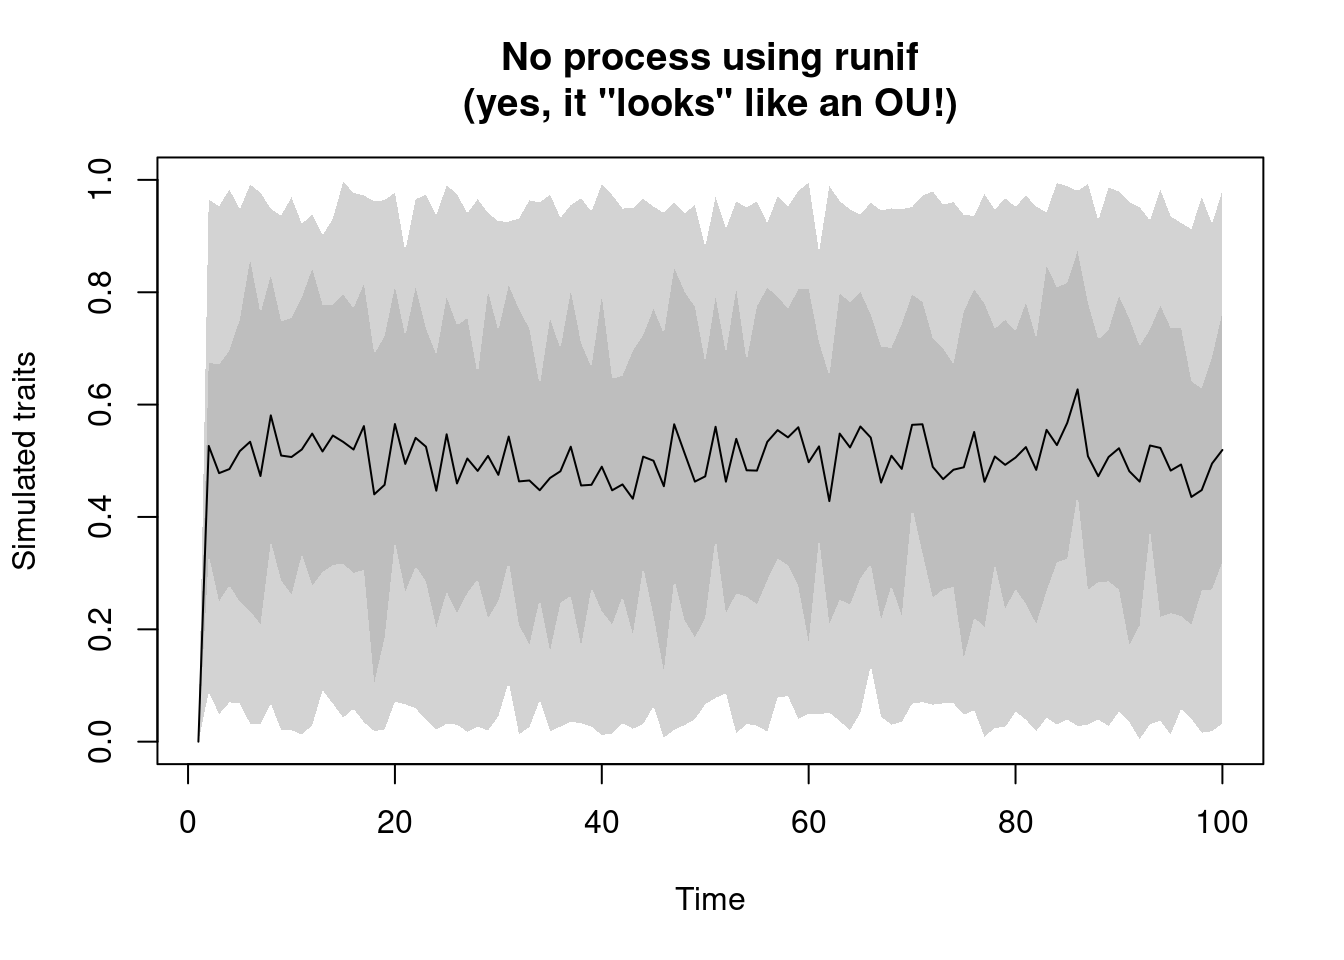
\includegraphics{treats_manual_files/figure-latex/unnamed-chunk-58-1.pdf}

\begin{itemize}
\tightlist
\item
  \texttt{multi.peak.process}: this process is a modified version of the \texttt{OU.process} that can take multiple local long-term mean values. The default OU process has one long-term mean towards which the values are drawn with the alpha parameter (the elastic band). The single long-term mean is usually 0. However, with this \texttt{multi.peak.process} we can set multiple values towards which values can be attracted with the same alpha parameter.
\end{itemize}

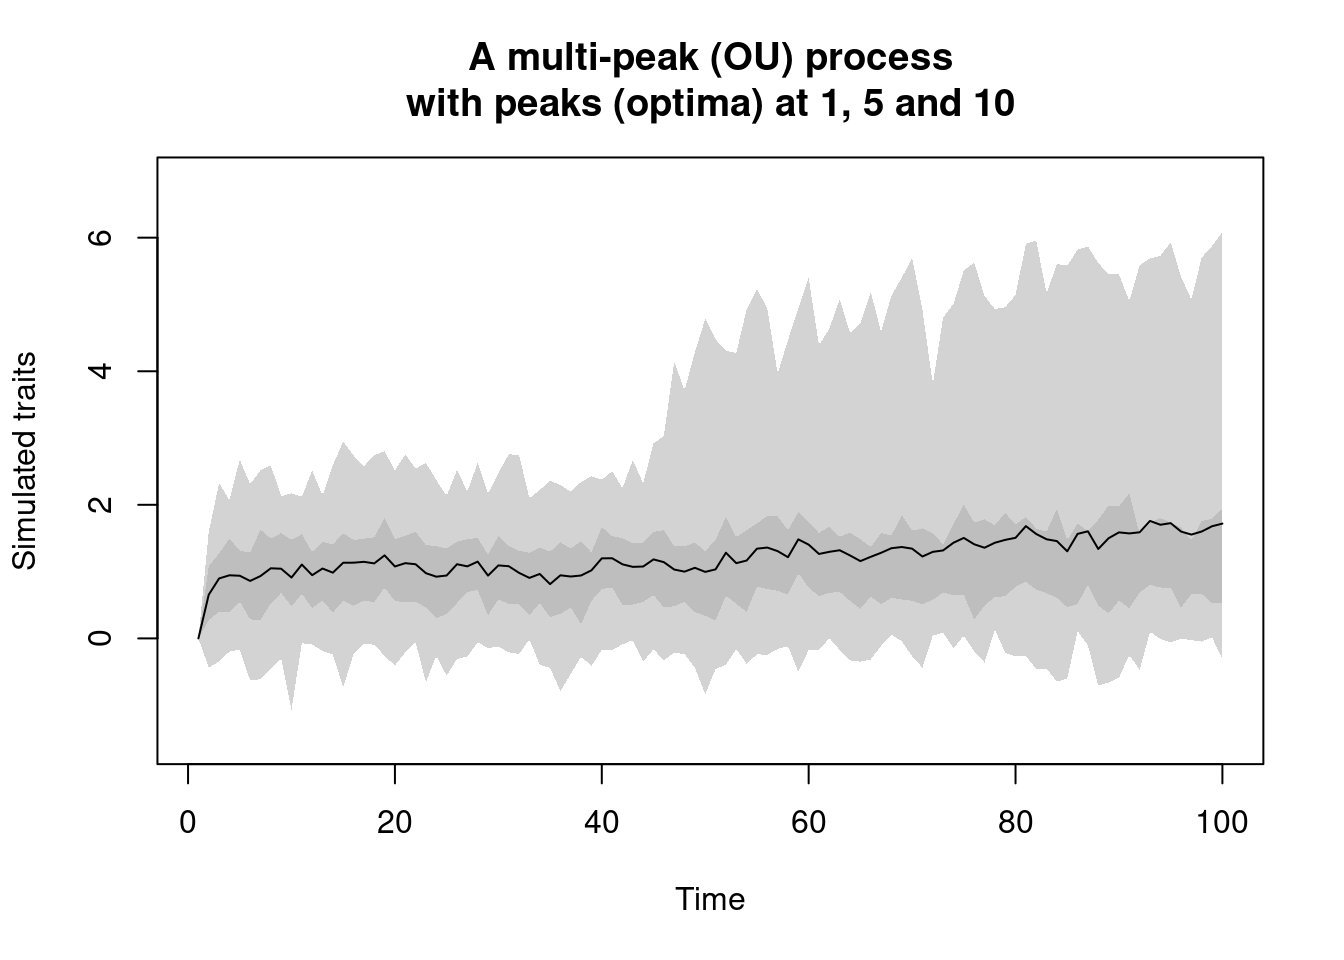
\includegraphics{treats_manual_files/figure-latex/unnamed-chunk-59-1.pdf}

\begin{itemize}
\tightlist
\item
  \texttt{repulsion.process}: this is a modified version of the \texttt{BM.process} where instead of accumulating gradually through time, new trait values are more likely to be different to the traits of their ancestor following a \texttt{repulsion} parameter.
\end{itemize}

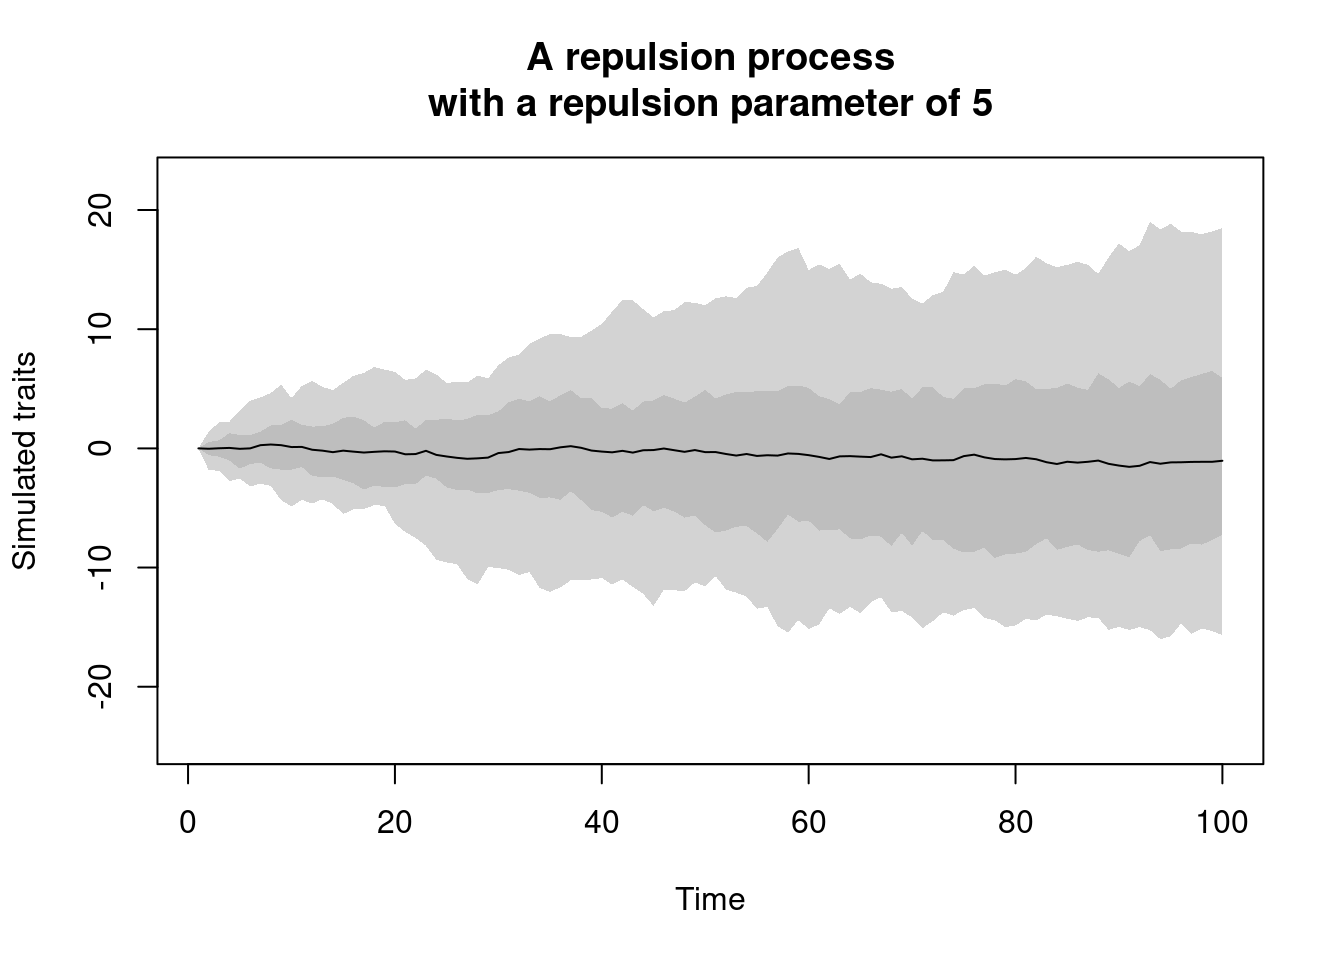
\includegraphics{treats_manual_files/figure-latex/unnamed-chunk-60-1.pdf}

\begin{itemize}
\tightlist
\item
  \texttt{discrete.process}: this one generates discrete trait values based on a transition matrix (you can use the utility function \texttt{transition.matrix} to generate one).
\end{itemize}

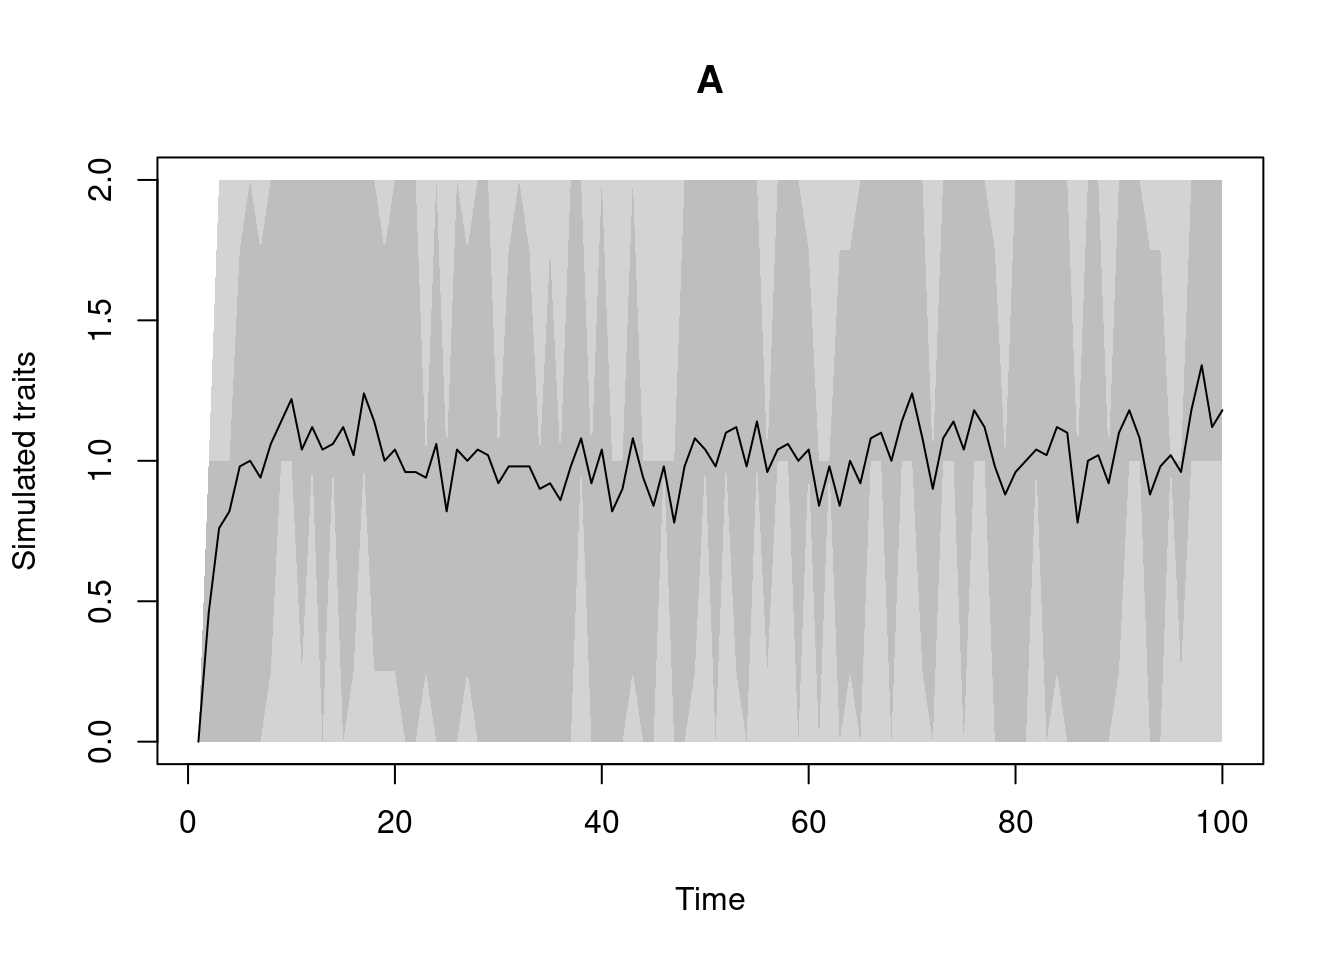
\includegraphics{treats_manual_files/figure-latex/unnamed-chunk-61-1.pdf}

Of course here the plotting of a discrete trait is not that informative\ldots{}

\hypertarget{testing-the-traits-with-test}{%
\section{\texorpdfstring{Testing the traits with \texttt{test}}{Testing the traits with test}}\label{testing-the-traits-with-test}}

\textbf{This bit is still in development.}
We highly suggest leaving \texttt{test\ =\ TRUE} so that \texttt{make.traits} returns an error if a process or its additional arguments (\texttt{process.args}) are not formatted correctly.
\texttt{make.traits} will send an error if the trait cannot be directly passed to \texttt{treats}.
However, in some specific cases (again, probably mainly for development and debugging) it could be useful to skip the tests using \texttt{test\ =\ FALSE}.

\hypertarget{mapping-traits-on-a-tree-map.traits}{%
\section{\texorpdfstring{Mapping traits on a tree: \texttt{map.traits}}{Mapping traits on a tree: map.traits}}\label{mapping-traits-on-a-tree-map.traits}}

Although \texttt{make.traits} is mainly designed for \texttt{treats} simulations, i.e.~simulating both the trees AND the traits at the same time, it is possible to use an already simulated or estimated tree and generating one or more traits on it using the \texttt{map.traits} function. This function takes the trait input as a \texttt{"traits"} object (from \texttt{make.traits}) and a tree topology with branch length. Note that you can also use \texttt{"traits"} objects with multiple or multi-dimensional traits as well as multiple phylogenies (\texttt{"multiPhylo"}).

\begin{Shaded}
\begin{Highlighting}[]
\CommentTok{\#\# Simulating a random tree with branch length}
\NormalTok{my\_tree \textless{}{-}}\StringTok{ }\KeywordTok{rtree}\NormalTok{(}\DecValTok{20}\NormalTok{)}

\CommentTok{\#\# Creating three different traits objects:}
\CommentTok{\#\# A Brownian Motion}
\NormalTok{bm\_process \textless{}{-}}\StringTok{ }\KeywordTok{make.traits}\NormalTok{(}\DataTypeTok{process =}\NormalTok{ BM.process)}
\CommentTok{\#\# An Ornstein{-}Uhlenbeck process}
\NormalTok{ou\_process \textless{}{-}}\StringTok{ }\KeywordTok{make.traits}\NormalTok{(}\DataTypeTok{process =}\NormalTok{ OU.process)}
\CommentTok{\#\# No process (just randomly drawing values from a normal distribution)}
\NormalTok{no\_process \textless{}{-}}\StringTok{ }\KeywordTok{make.traits}\NormalTok{(}\DataTypeTok{process =}\NormalTok{ no.process)}

\CommentTok{\#\# Mapping the three traits on the phylogeny}
\NormalTok{bm\_traits \textless{}{-}}\StringTok{ }\KeywordTok{map.traits}\NormalTok{(bm\_process, my\_tree)}
\NormalTok{ou\_traits \textless{}{-}}\StringTok{ }\KeywordTok{map.traits}\NormalTok{(ou\_process, my\_tree)}
\NormalTok{no\_traits \textless{}{-}}\StringTok{ }\KeywordTok{map.traits}\NormalTok{(no\_process, my\_tree)}

\CommentTok{\#\# Plotting the topology and the different traits}
\KeywordTok{par}\NormalTok{(}\DataTypeTok{mfrow =} \KeywordTok{c}\NormalTok{(}\DecValTok{2}\NormalTok{,}\DecValTok{2}\NormalTok{))}
\KeywordTok{plot}\NormalTok{(my\_tree, }\DataTypeTok{main =} \StringTok{"Base topology"}\NormalTok{)}
\KeywordTok{plot}\NormalTok{(bm\_traits, }\DataTypeTok{main =} \StringTok{"Mapped BM"}\NormalTok{)}
\KeywordTok{plot}\NormalTok{(ou\_traits, }\DataTypeTok{main =} \StringTok{"Mapped OU"}\NormalTok{)}
\KeywordTok{plot}\NormalTok{(no\_traits, }\DataTypeTok{main =} \StringTok{"Mapped normal trait"}\NormalTok{)}
\end{Highlighting}
\end{Shaded}

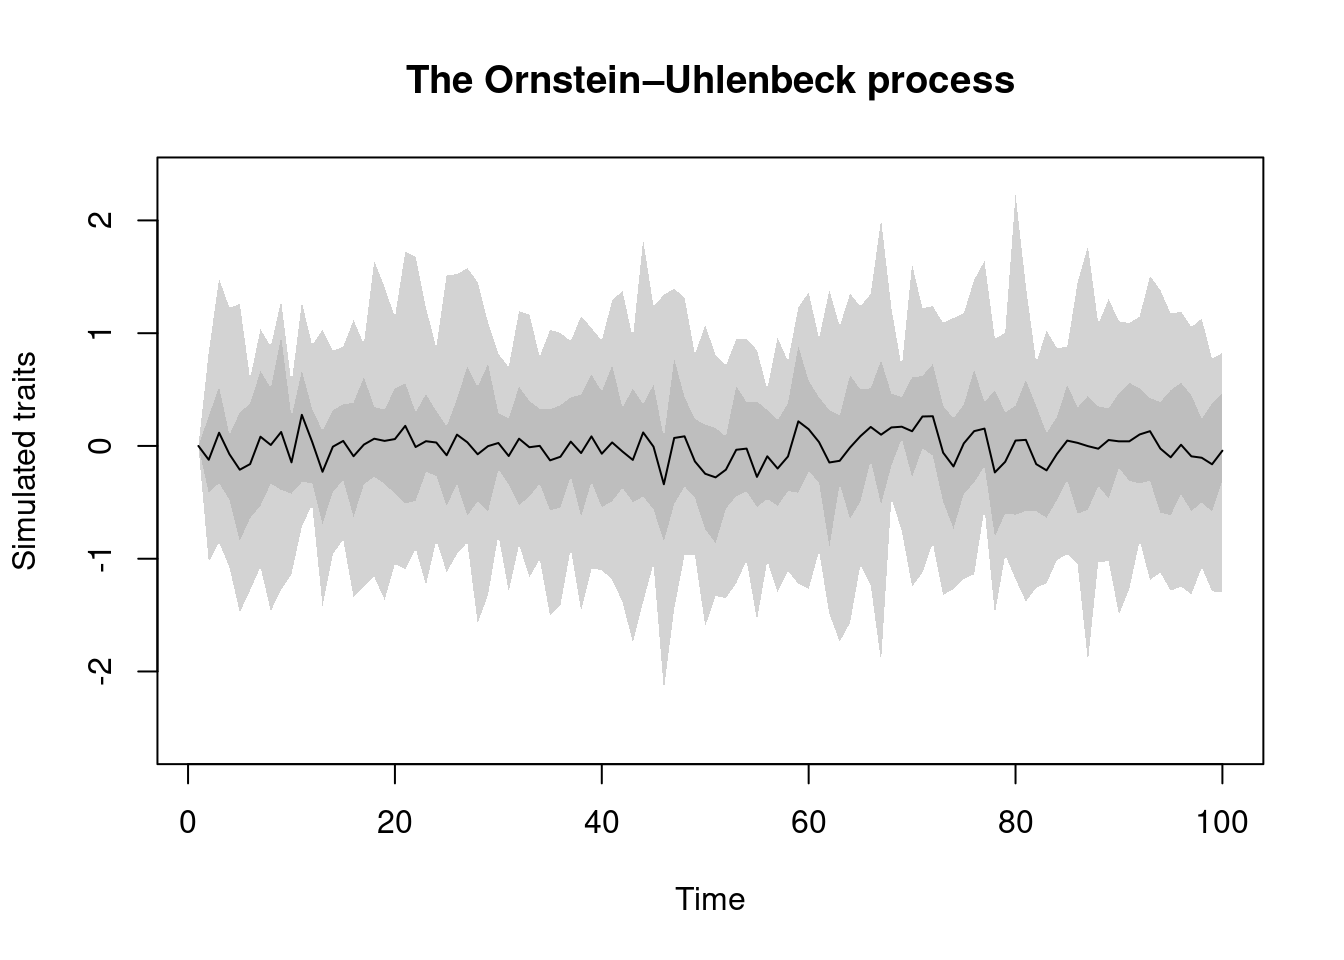
\includegraphics{treats_manual_files/figure-latex/unnamed-chunk-62-1.pdf}

\hypertarget{templates-for-making-your-very-own-process}{%
\section{Templates for making your very own process}\label{templates-for-making-your-very-own-process}}

As detailed above, any process of your own design will work as long as it is a function that takes at least the arguments \texttt{x0} and \texttt{edge.length}.
You can be imaginative and creative when designing your own process but here are two detailed example functions for a unidimensional Brownian Motion and Ornstein-Uhlenbeck process that you can use for a start (or not).
Remember it is good practice for \texttt{treats} processes to set all the arguments with default values (just in case).

\begin{quote}
Note that the functions below are not equal to the already implemented \texttt{BM.process} and \texttt{OU.process} but an easier to edit version that you can use as a template:
\end{quote}

\hypertarget{a-simple-brownian-motion-process-template}{%
\subsection{A simple Brownian Motion process template}\label{a-simple-brownian-motion-process-template}}

\begin{Shaded}
\begin{Highlighting}[]
\CommentTok{\#\# A simple Brownian motion process}
\NormalTok{my.BM.process \textless{}{-}}\StringTok{ }\ControlFlowTok{function}\NormalTok{(}\DataTypeTok{x0 =} \DecValTok{0}\NormalTok{, }\DataTypeTok{edge.length =} \DecValTok{1}\NormalTok{, }\DataTypeTok{sd =} \DecValTok{1}\NormalTok{, ...) \{}
    \CommentTok{\#\# Drawing a random number from a normal distribution}
    \CommentTok{\#\# with x0 as the and a given standard deviation}
    \CommentTok{\#\# and depending on branch (edge) length}
\NormalTok{    result \textless{}{-}}\StringTok{ }\KeywordTok{rnorm}\NormalTok{(}\DataTypeTok{n =} \DecValTok{1}\NormalTok{, }\DataTypeTok{mean =}\NormalTok{ x0, }\DataTypeTok{sd =} \KeywordTok{sqrt}\NormalTok{(sd}\OperatorTok{\^{}}\DecValTok{2} \OperatorTok{*}\StringTok{ }\NormalTok{edge.length))}

    \CommentTok{\#\# Return the number}
    \KeywordTok{return}\NormalTok{(result)}
\NormalTok{\}}
\end{Highlighting}
\end{Shaded}

\hypertarget{a-simple-ornstein-uhlenbeck-process-template}{%
\subsection{A simple Ornstein-Uhlenbeck process template}\label{a-simple-ornstein-uhlenbeck-process-template}}

\begin{Shaded}
\begin{Highlighting}[]
\CommentTok{\#\# A simple Ornstein{-}Uhlenbeck motion process}
\NormalTok{my.OU.process \textless{}{-}}\StringTok{ }\ControlFlowTok{function}\NormalTok{(}\DataTypeTok{x0 =} \DecValTok{0}\NormalTok{, }\DataTypeTok{edge.length =} \DecValTok{1}\NormalTok{, }\DataTypeTok{var =} \DecValTok{1}\NormalTok{, }\DataTypeTok{alpha =} \DecValTok{1}\NormalTok{, ...) \{}
    \CommentTok{\#\# Calculate the mean based on alpha}
\NormalTok{    mean \textless{}{-}}\StringTok{ }\NormalTok{x0 }\OperatorTok{*}\StringTok{ }\KeywordTok{exp}\NormalTok{(}\OperatorTok{{-}}\NormalTok{alpha)}
    \CommentTok{\#\# Calculate the standard deviation based on alpha and the variance}
\NormalTok{    sd \textless{}{-}}\StringTok{ }\KeywordTok{sqrt}\NormalTok{(var}\OperatorTok{/}\NormalTok{(}\DecValTok{2} \OperatorTok{*}\StringTok{ }\NormalTok{alpha) }\OperatorTok{*}\StringTok{ }\NormalTok{(}\DecValTok{1} \OperatorTok{{-}}\StringTok{ }\KeywordTok{exp}\NormalTok{(}\OperatorTok{{-}}\DecValTok{2} \OperatorTok{*}\StringTok{ }\NormalTok{alpha)))}
    \CommentTok{\#\# Draw a random number from a normal distribution}
    \CommentTok{\#\# using this mean and standard deviation}
    \CommentTok{\#\# and depending on branch (edge) length}
\NormalTok{    result \textless{}{-}}\StringTok{ }\KeywordTok{rnorm}\NormalTok{(}\DataTypeTok{n =} \DecValTok{1}\NormalTok{, }\DataTypeTok{mean =}\NormalTok{ mean, }\DataTypeTok{sd =} \KeywordTok{sqrt}\NormalTok{(sd}\OperatorTok{\^{}}\DecValTok{2} \OperatorTok{*}\StringTok{ }\NormalTok{edge.length))}

    \CommentTok{\#\# Return the number}
    \KeywordTok{return}\NormalTok{(result)}
\NormalTok{\}}
\end{Highlighting}
\end{Shaded}

\hypertarget{makemodifiers}{%
\chapter{Modifying the birth-death process}\label{makemodifiers}}

\texttt{"modifiers"} have a similar structure than \texttt{"traits"} where you can design an object with increasing complexity, starting with the simplest modifiers that doesn't modify anything (using the default arguments):

\begin{Shaded}
\begin{Highlighting}[]
\CommentTok{\#\# Making a default modifier (no modification)}
\NormalTok{my\_default\_modifiers \textless{}{-}}\StringTok{ }\KeywordTok{make.modifiers}\NormalTok{()}
\NormalTok{my\_default\_modifiers}
\end{Highlighting}
\end{Shaded}

\begin{verbatim}
##  ---- treats modifiers object ---- 
## No modifiers applied to the branch length, selection and speciation processes (default).
\end{verbatim}

Similarly to \texttt{"traits"} objects, \texttt{"modifiers"} are also printed by default using \texttt{print.treats}.
You can see details about what's actually in the object using \texttt{print.treats(my\_default\_modifiers,\ all\ =\ TRUE)}.
However, contrary to \texttt{"traits"}, you cannot plot \texttt{"modifiers"}.

\begin{figure}
\centering
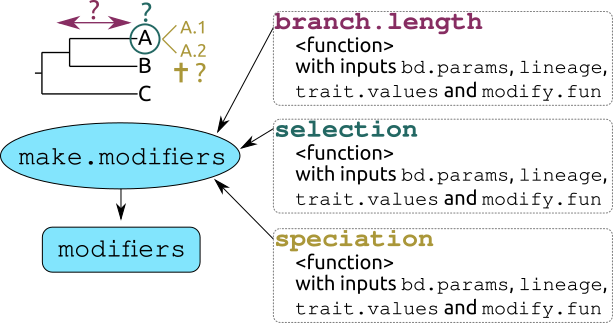
\includegraphics{make.modifiers.png}
\caption{\texttt{make.modifiers}: The three main inputs to make modifiers are functions to modify the \texttt{branch.length} (waiting) process controlling the ``growth'' of the tree; the \texttt{selection} (selecting) process controlling the selection of the tip on which to apply speciation or extinction; and the \texttt{speciation} (speciating) process controlling whether the select tip goes extinct or speciates. The allowed arguments are detailed \protect\hyperlink{allowarguments}{here}.}
\end{figure}

\hypertarget{quick-overview-1}{%
\subsection{Quick overview}\label{quick-overview-1}}

\begin{longtable}[]{@{}llll@{}}
\toprule
\begin{minipage}[b]{0.19\columnwidth}\raggedright
function\strut
\end{minipage} & \begin{minipage}[b]{0.23\columnwidth}\raggedright
arguments\strut
\end{minipage} & \begin{minipage}[b]{0.14\columnwidth}\raggedright
input\strut
\end{minipage} & \begin{minipage}[b]{0.33\columnwidth}\raggedright
what does it do\strut
\end{minipage}\tabularnewline
\midrule
\endhead
\begin{minipage}[t]{0.19\columnwidth}\raggedright
\texttt{make.modifiers}\strut
\end{minipage} & \begin{minipage}[t]{0.23\columnwidth}\raggedright
branch.length\strut
\end{minipage} & \begin{minipage}[t]{0.14\columnwidth}\raggedright
a function\strut
\end{minipage} & \begin{minipage}[t]{0.33\columnwidth}\raggedright
generating branch length (see below)\strut
\end{minipage}\tabularnewline
\begin{minipage}[t]{0.19\columnwidth}\raggedright
\texttt{make.modifiers}\strut
\end{minipage} & \begin{minipage}[t]{0.23\columnwidth}\raggedright
selection\strut
\end{minipage} & \begin{minipage}[t]{0.14\columnwidth}\raggedright
a function\strut
\end{minipage} & \begin{minipage}[t]{0.33\columnwidth}\raggedright
selecting a lineage (see below)\strut
\end{minipage}\tabularnewline
\begin{minipage}[t]{0.19\columnwidth}\raggedright
\texttt{make.modifiers}\strut
\end{minipage} & \begin{minipage}[t]{0.23\columnwidth}\raggedright
speciation\strut
\end{minipage} & \begin{minipage}[t]{0.14\columnwidth}\raggedright
a function\strut
\end{minipage} & \begin{minipage}[t]{0.33\columnwidth}\raggedright
choosing between speciation and extinction (see below)\strut
\end{minipage}\tabularnewline
\begin{minipage}[t]{0.19\columnwidth}\raggedright
\texttt{make.modifiers}\strut
\end{minipage} & \begin{minipage}[t]{0.23\columnwidth}\raggedright
condition\strut
\end{minipage} & \begin{minipage}[t]{0.14\columnwidth}\raggedright
a function\strut
\end{minipage} & \begin{minipage}[t]{0.33\columnwidth}\raggedright
a function that affects the condition of when to trigger the functions above (see below)\strut
\end{minipage}\tabularnewline
\begin{minipage}[t]{0.19\columnwidth}\raggedright
\texttt{make.modifiers}\strut
\end{minipage} & \begin{minipage}[t]{0.23\columnwidth}\raggedright
modify\strut
\end{minipage} & \begin{minipage}[t]{0.14\columnwidth}\raggedright
a function\strut
\end{minipage} & \begin{minipage}[t]{0.33\columnwidth}\raggedright
a function that modifies the value of the trigger value generated when the \texttt{condition} is met (see below)\strut
\end{minipage}\tabularnewline
\begin{minipage}[t]{0.19\columnwidth}\raggedright
\texttt{make.modifiers}\strut
\end{minipage} & \begin{minipage}[t]{0.23\columnwidth}\raggedright
add\strut
\end{minipage} & \begin{minipage}[t]{0.14\columnwidth}\raggedright
a \texttt{treats} object\strut
\end{minipage} & \begin{minipage}[t]{0.33\columnwidth}\raggedright
another modifier generated by \texttt{make.modifiers}\strut
\end{minipage}\tabularnewline
\begin{minipage}[t]{0.19\columnwidth}\raggedright
\texttt{make.modifiers}\strut
\end{minipage} & \begin{minipage}[t]{0.23\columnwidth}\raggedright
update\strut
\end{minipage} & \begin{minipage}[t]{0.14\columnwidth}\raggedright
a \texttt{treats} object\strut
\end{minipage} & \begin{minipage}[t]{0.33\columnwidth}\raggedright
another modifier generated by \texttt{make.modifiers}\strut
\end{minipage}\tabularnewline
\begin{minipage}[t]{0.19\columnwidth}\raggedright
\texttt{make.modifiers}\strut
\end{minipage} & \begin{minipage}[t]{0.23\columnwidth}\raggedright
test\strut
\end{minipage} & \begin{minipage}[t]{0.14\columnwidth}\raggedright
logical\strut
\end{minipage} & \begin{minipage}[t]{0.33\columnwidth}\raggedright
whether to test the validity of the modifier\strut
\end{minipage}\tabularnewline
\begin{minipage}[t]{0.19\columnwidth}\raggedright
---------\strut
\end{minipage} & \begin{minipage}[t]{0.23\columnwidth}\raggedright
-----------\strut
\end{minipage} & \begin{minipage}[t]{0.14\columnwidth}\raggedright
-------\strut
\end{minipage} & \begin{minipage}[t]{0.33\columnwidth}\raggedright
----------------\strut
\end{minipage}\tabularnewline
\begin{minipage}[t]{0.19\columnwidth}\raggedright
\texttt{branch.length}, \texttt{selection}, \texttt{speciation}, \texttt{condition}\strut
\end{minipage} & \begin{minipage}[t]{0.23\columnwidth}\raggedright
bd.params\strut
\end{minipage} & \begin{minipage}[t]{0.14\columnwidth}\raggedright
a \texttt{treats} object generated by \texttt{make.bd.params}\strut
\end{minipage} & \begin{minipage}[t]{0.33\columnwidth}\raggedright
usually handled internally (contains the either the birth-death values or their distribution)\strut
\end{minipage}\tabularnewline
\begin{minipage}[t]{0.19\columnwidth}\raggedright
\ldots{}\strut
\end{minipage} & \begin{minipage}[t]{0.23\columnwidth}\raggedright
lineage\strut
\end{minipage} & \begin{minipage}[t]{0.14\columnwidth}\raggedright
a named ``lineage'' list\strut
\end{minipage} & \begin{minipage}[t]{0.33\columnwidth}\raggedright
usually handled internally (contains the current state of the simulations)\strut
\end{minipage}\tabularnewline
\begin{minipage}[t]{0.19\columnwidth}\raggedright
\ldots{}\strut
\end{minipage} & \begin{minipage}[t]{0.23\columnwidth}\raggedright
trait.values\strut
\end{minipage} & \begin{minipage}[t]{0.14\columnwidth}\raggedright
a matrix\strut
\end{minipage} & \begin{minipage}[t]{0.33\columnwidth}\raggedright
usually handled internally (contains the current generated traits of the simulations)\strut
\end{minipage}\tabularnewline
\bottomrule
\end{longtable}

\hypertarget{the-default-modifier-how-the-process-is-working}{%
\section{The default modifier (how the process is working)}\label{the-default-modifier-how-the-process-is-working}}

The modifiers modify the core of the birth-death process as implemented in \texttt{treats}.
By default, the birth-death process in \texttt{treats} uses this modifier:

\begin{Shaded}
\begin{Highlighting}[]
\CommentTok{\#\# What is actually in the default modifier?}
\KeywordTok{print}\NormalTok{(}\KeywordTok{make.modifiers}\NormalTok{(), }\DataTypeTok{all =} \OtherTok{TRUE}\NormalTok{)}
\end{Highlighting}
\end{Shaded}

\begin{verbatim}
## $waiting
## $waiting$fun
## function (bd.params, lineage = NULL, trait.values = NULL, modify.fun = NULL) 
## {
##     return(rexp(1, sum(lineage$n * (bd.params$speciation + bd.params$extinction))))
## }
## <bytecode: 0x609b211b6680>
## <environment: namespace:treats>
## 
## $waiting$internal
## NULL
## 
## 
## $selecting
## $selecting$fun
## function (bd.params, lineage = NULL, trait.values = NULL, modify.fun = NULL) 
## {
##     return(sample(lineage$n, 1))
## }
## <bytecode: 0x609b211694e0>
## <environment: namespace:treats>
## 
## $selecting$internal
## NULL
## 
## 
## $speciating
## $speciating$fun
## function (bd.params, lineage = NULL, trait.values = NULL, modify.fun = NULL) 
## {
##     return(runif(1) <= (bd.params$speciation/(bd.params$speciation + 
##         bd.params$extinction)))
## }
## <bytecode: 0x609b21164168>
## <environment: namespace:treats>
## 
## $speciating$internal
## NULL
## 
## 
## $call
## $call$waiting
## $call$waiting$fun
## [1] "default"
## 
## 
## $call$selecting
## $call$selecting$fun
## [1] "default"
## 
## 
## $call$speciating
## $call$speciating$fun
## [1] "default"
\end{verbatim}

This contains a lot of information, much of it is actually not useful for using the modular aspects of \texttt{treats} at a high user level, i.e.~unless you want to code very specific things, you won't need most of the information. The essentials are these three functions in the elements named \texttt{"waiting\$fun"}, \texttt{"selecting\$fun"} and \texttt{"speciating\$fun"}:

\begin{enumerate}
\def\labelenumi{\arabic{enumi}.}
\tightlist
\item
  \texttt{"waiting\$fun"} is the branch length function (defined in detail below) which returns a randomly drawn number from an exponential distribution with the rate of the number of taxa multiplied by the speciation and extinction rate: \(n \times (\lambda + \mu)\) (here is uses the extra function \texttt{sum} for internal modularity reasons). \textbf{This function is responsible for the growth of the length/age of the tree}
\end{enumerate}

\begin{Shaded}
\begin{Highlighting}[]
\KeywordTok{rexp}\NormalTok{(}\DecValTok{1}\NormalTok{, }\KeywordTok{sum}\NormalTok{(lineage}\OperatorTok{$}\NormalTok{n }\OperatorTok{*}\StringTok{ }\NormalTok{(bd.params}\OperatorTok{$}\NormalTok{speciation }\OperatorTok{+}\StringTok{ }\NormalTok{bd.params}\OperatorTok{$}\NormalTok{extinction)))}
\end{Highlighting}
\end{Shaded}

With \texttt{lineage\$n} being the number of lineages and \texttt{bd.params\$speciation} and \texttt{bd.params\$extinction} the speciation and extinction parameters (these specific terms are defined in detail below).

\begin{enumerate}
\def\labelenumi{\arabic{enumi}.}
\setcounter{enumi}{1}
\tightlist
\item
  \texttt{"selecting\$fun"} is the selection function (defined in detail below) which, after the waiting time defined above returns a randomly selected lineage (a tip) among the existing ones. \textbf{This function is responsible for the branch selection}.
\end{enumerate}

\begin{Shaded}
\begin{Highlighting}[]
\KeywordTok{sample}\NormalTok{(lineage}\OperatorTok{$}\NormalTok{n, }\DecValTok{1}\NormalTok{)}
\end{Highlighting}
\end{Shaded}

\begin{enumerate}
\def\labelenumi{\arabic{enumi}.}
\setcounter{enumi}{2}
\tightlist
\item
  \texttt{"speciating\$fun"} is the speciation function (defined in detail below) which randomly draws a number (\texttt{runif(1)}) and depending on the speciation and extinction parameters makes the selected lineage (from 2.) speciate (\texttt{TRUE}) or go extinct (\texttt{FALSE}). \textbf{This function is responsible for the speciation or extinction of species}.
\end{enumerate}

\begin{Shaded}
\begin{Highlighting}[]
\KeywordTok{runif}\NormalTok{(}\DecValTok{1}\NormalTok{) }\OperatorTok{\textless{}}\StringTok{ }\NormalTok{(bd.params}\OperatorTok{$}\NormalTok{speciation}\OperatorTok{/}\NormalTok{(bd.params}\OperatorTok{$}\NormalTok{speciation }\OperatorTok{+}\StringTok{ }\NormalTok{bd.params}\OperatorTok{$}\NormalTok{extinction))}
\end{Highlighting}
\end{Shaded}

We will have a look at all these aspects below in more detail which should make things clearer (but you can always refer to the default here for information).

\hypertarget{the-branch-length-function-branch.length}{%
\section{\texorpdfstring{The branch length function (\texttt{branch.length})}{The branch length function (branch.length)}}\label{the-branch-length-function-branch.length}}

The first argument in \texttt{"modifiers"} is the branch length function (\texttt{branch.length}) this is the function that will be executed in \texttt{treats} to generate branch lengths.
Note that in the \texttt{treats} algorithm, branch length is not generated \emph{directly} but as the result of the waiting time.
In other words, the \texttt{branch.length} function just affects waiting time for all taxa present at any time in the simulation.
These taxa can then either go extinct (stopping the ``growth'' of its branch length) or survive (continuing the ``growth'').

By default, branch length (or waiting/growth) is a randomly drawn number from an exponential distribution with the rate of the number of taxa multiplied by the speciation and extinction rate: \(n \times (\lambda + \mu)\) (where \(n\) is the number of taxa currently present in the simulation, \(\lambda\) and \(\mu\) are respectively the speciation and extinction rates).
This default function is simply called \texttt{branch.length} in \texttt{treats} and can be used as a modifier as follows:

\begin{Shaded}
\begin{Highlighting}[]
\CommentTok{\#\# Specifying the default modifier}
\NormalTok{default\_modifiers \textless{}{-}}\StringTok{ }\KeywordTok{make.modifiers}\NormalTok{(}\DataTypeTok{branch.length =}\NormalTok{ branch.length)}

\CommentTok{\#\# Setting some parameters for generating trees}
\NormalTok{bd\_params \textless{}{-}}\StringTok{ }\KeywordTok{list}\NormalTok{(}\DataTypeTok{extinction =} \DecValTok{0}\NormalTok{)}
\NormalTok{stop\_rule \textless{}{-}}\StringTok{ }\KeywordTok{list}\NormalTok{(}\DataTypeTok{max.living =} \DecValTok{20}\NormalTok{)}

\CommentTok{\#\# Generating a tree with the default branch length parameter}
\KeywordTok{set.seed}\NormalTok{(}\DecValTok{0}\NormalTok{)}
\NormalTok{default\_tree \textless{}{-}}\StringTok{ }\KeywordTok{treats}\NormalTok{(}\DataTypeTok{bd.params =}\NormalTok{ bd\_params,}
                     \DataTypeTok{stop.rule =}\NormalTok{ stop\_rule,}
                     \DataTypeTok{modifiers =}\NormalTok{ default\_modifiers)}
\end{Highlighting}
\end{Shaded}

Of course, the point of the modularity here is that you can provide your own function for generating branch length.
For example, we might be interested in what our tree would look like if we use a simple constant branch length generation (instead of randomly drawing it from an exponential distribution).
We can do so by declaring our own \texttt{branch.length} function and adding it to a \texttt{"modifiers"} object.

\begin{Shaded}
\begin{Highlighting}[]
\CommentTok{\#\# A constant branch length generator}
\CommentTok{\#\# (note that the output must be numeric, not integer)}
\NormalTok{constant.brlen \textless{}{-}}\StringTok{ }\ControlFlowTok{function}\NormalTok{() \{}
    \KeywordTok{return}\NormalTok{(}\KeywordTok{as.numeric}\NormalTok{(}\DecValTok{1}\NormalTok{))}
\NormalTok{\}}

\CommentTok{\#\# Creating the modifiers object}
\NormalTok{constant\_modifier \textless{}{-}}\StringTok{ }\KeywordTok{make.modifiers}\NormalTok{(}\DataTypeTok{branch.length =}\NormalTok{ constant.brlen)}

\CommentTok{\#\# Generating a new tree with this modifier}
\KeywordTok{set.seed}\NormalTok{(}\DecValTok{0}\NormalTok{)}
\NormalTok{modified\_tree \textless{}{-}}\StringTok{ }\KeywordTok{treats}\NormalTok{(}\DataTypeTok{bd.params =}\NormalTok{ bd\_params,}
                      \DataTypeTok{stop.rule =}\NormalTok{ stop\_rule,}
                      \DataTypeTok{modifiers =}\NormalTok{ constant\_modifier)}
\end{Highlighting}
\end{Shaded}

And we can visualise the difference between both resulting trees:

\begin{Shaded}
\begin{Highlighting}[]
\KeywordTok{par}\NormalTok{(}\DataTypeTok{mfrow =} \KeywordTok{c}\NormalTok{(}\DecValTok{1}\NormalTok{,}\DecValTok{2}\NormalTok{))}
\KeywordTok{plot}\NormalTok{(default\_tree,  }\DataTypeTok{main =} \StringTok{"Default modifier"}\NormalTok{)}
\KeywordTok{plot}\NormalTok{(modified\_tree, }\DataTypeTok{main =} \StringTok{"Constant branch length}\CharTok{\textbackslash{}n}\StringTok{modifier"}\NormalTok{)}
\end{Highlighting}
\end{Shaded}

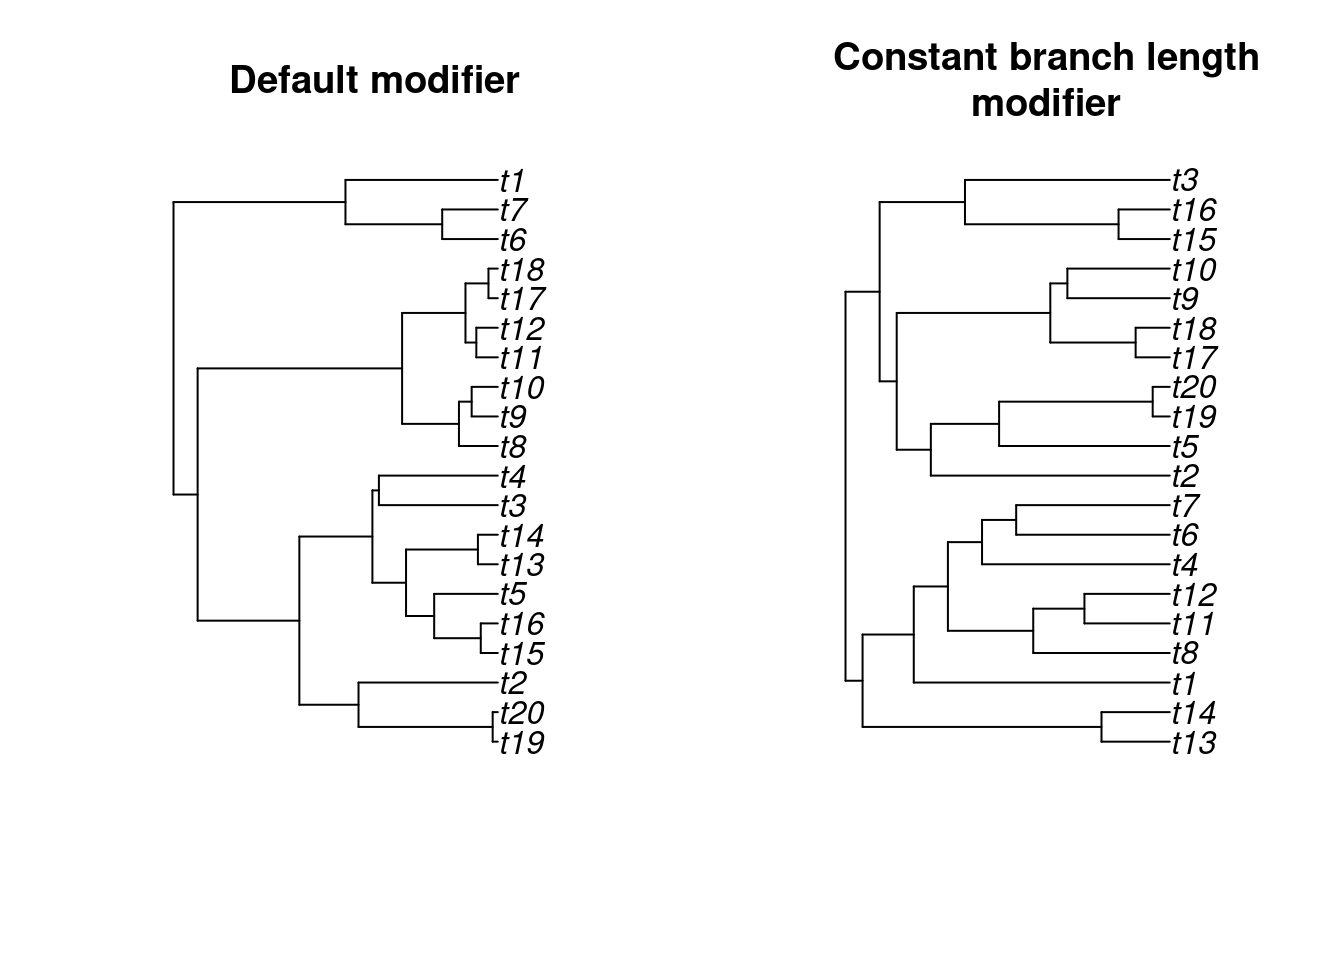
\includegraphics{treats_manual_files/figure-latex/unnamed-chunk-73-1.pdf}

\begin{Shaded}
\begin{Highlighting}[]
\KeywordTok{par}\NormalTok{(}\DataTypeTok{mfrow =} \KeywordTok{c}\NormalTok{(}\DecValTok{1}\NormalTok{,}\DecValTok{1}\NormalTok{))}
\end{Highlighting}
\end{Shaded}

It is of course possible to use more complex branch length modifiers that take different conditions and specific modification rather than simply always outputing a value of one.

\hypertarget{allowarguments}{%
\subsection{The modifier arguments}\label{allowarguments}}

You can create a function for \texttt{branch.length}, \texttt{selection} and \texttt{speciation} that involve any of the following arguments:

\begin{itemize}
\tightlist
\item
  \texttt{bd.params}: a named list containing \texttt{"numeric"} values that contains the birth-death parameters (at least \texttt{"speciation"} and \texttt{"extinction"});
\item
  \texttt{lineage}: a named list containing the lineage data (see below).
\item
  \texttt{trait.values}: a \texttt{"matrix"} containing \texttt{"numeric"} values with the trait names as column names and the lineage ID as row numbers (you can use it with the function \texttt{parent.traits} to access the trait of the previous node for example).
\item
  \texttt{modify.fun}: a \texttt{"list"} of named \texttt{"function"} (usually passed through \texttt{condition} and \texttt{modify}).
\end{itemize}

The \texttt{lineage} list contains the following elements (missing elements are allowed):

\begin{itemize}
\tightlist
\item
  \texttt{lineage\$parents}: an \texttt{"integer"} vector: the list of parent lineages;
\item
  \texttt{lineage\$livings}: an \texttt{"integer"} vector: the list of lineages still not extinct;
\item
  \texttt{lineage\$drawn}: a single \texttt{"integer"}: the ID of the selected lineage; this must be a number in \texttt{1:lineage\$n};
\item
  \texttt{lineage\$current}: a single \texttt{"integer"}: the selected lineage (is equal to \texttt{lineage\$livings{[}lineage\$drawn{]}});
\item
  \texttt{lineage\$n}: a single \texttt{"integer"}: the current number of non extinct lineage (is equal to \texttt{length(lineage\$livings))};
\item
  \texttt{lineage\$split}: a \texttt{"logical"} vector: the list of splits for each lineage (\texttt{TRUE}), the number of total tips is equal to \texttt{sum(!lineage\$split)}.
\end{itemize}

In general, unless you know what you're doing, you can ignore most arguments for specific modifiers since they are handled automatically within the \texttt{treats} function.
Therefore any argument can be left undeclared or missing and is always handled internally. For example, if you did not declare \texttt{lineage\$n} as a function argument but are using \texttt{lineage\$n} in the function, \texttt{lineage\$n} will be detected and treated as a current argument automatically as set accordingly within the birth-death process (e.g.~\texttt{lineage\$n} will be set to the current number of taxa every iteration of the process).

For example, we can create a function that increases branch length proportional to the number of species ``alive'' at each time of the simulation in a discrete way, i.e.~for discrete numbers of taxa, the branch length increases by jumps (ten fold) every five taxa:

\begin{Shaded}
\begin{Highlighting}[]
\CommentTok{\#\# A more complex binned.branch.length function}
\NormalTok{increasing.brlen \textless{}{-}}\StringTok{ }\ControlFlowTok{function}\NormalTok{(bd.params, lineage) \{}

    \CommentTok{\#\# Setting the cumulated birth and death}
\NormalTok{    birth\_death \textless{}{-}}\StringTok{ }\NormalTok{bd.params}\OperatorTok{$}\NormalTok{speciation }\OperatorTok{+}\StringTok{ }\NormalTok{bd.params}\OperatorTok{$}\NormalTok{extinction}

    \CommentTok{\#\# Returning branch lengths depending on different number of taxa}
    \ControlFlowTok{if}\NormalTok{(lineage}\OperatorTok{$}\NormalTok{n }\OperatorTok{\textless{}=}\StringTok{ }\DecValTok{5}\NormalTok{) \{}
        \KeywordTok{return}\NormalTok{(}\DecValTok{1}    \OperatorTok{*}\StringTok{ }\KeywordTok{rexp}\NormalTok{(}\DecValTok{1}\NormalTok{, }\KeywordTok{sum}\NormalTok{(}\DecValTok{5} \OperatorTok{*}\StringTok{ }\NormalTok{birth\_death)))}
\NormalTok{    \}}
    \ControlFlowTok{if}\NormalTok{(lineage}\OperatorTok{$}\NormalTok{n }\OperatorTok{\textless{}=}\StringTok{ }\DecValTok{10}\NormalTok{) \{}
        \KeywordTok{return}\NormalTok{(}\DecValTok{10}   \OperatorTok{*}\StringTok{ }\KeywordTok{rexp}\NormalTok{(}\DecValTok{1}\NormalTok{, }\KeywordTok{sum}\NormalTok{(}\DecValTok{10} \OperatorTok{*}\StringTok{ }\NormalTok{birth\_death)))   }
\NormalTok{    \}}
    \ControlFlowTok{if}\NormalTok{(lineage}\OperatorTok{$}\NormalTok{n }\OperatorTok{\textless{}=}\StringTok{ }\DecValTok{15}\NormalTok{) \{}
        \KeywordTok{return}\NormalTok{(}\DecValTok{100}  \OperatorTok{*}\StringTok{ }\KeywordTok{rexp}\NormalTok{(}\DecValTok{1}\NormalTok{, }\KeywordTok{sum}\NormalTok{(}\DecValTok{15} \OperatorTok{*}\StringTok{ }\NormalTok{birth\_death)))      }
\NormalTok{    \}}
    \ControlFlowTok{if}\NormalTok{(lineage}\OperatorTok{$}\NormalTok{n }\OperatorTok{\textless{}=}\StringTok{ }\DecValTok{20}\NormalTok{) \{}
        \KeywordTok{return}\NormalTok{(}\DecValTok{1000} \OperatorTok{*}\StringTok{ }\KeywordTok{rexp}\NormalTok{(}\DecValTok{1}\NormalTok{, }\KeywordTok{sum}\NormalTok{(}\DecValTok{20} \OperatorTok{*}\StringTok{ }\NormalTok{birth\_death)))}
\NormalTok{    \} }\ControlFlowTok{else}\NormalTok{ \{}
        \KeywordTok{return}\NormalTok{(}\DecValTok{1000} \OperatorTok{*}\StringTok{ }\KeywordTok{rexp}\NormalTok{(}\DecValTok{1}\NormalTok{, }\KeywordTok{sum}\NormalTok{(lineage}\OperatorTok{$}\NormalTok{n }\OperatorTok{*}\StringTok{ }\NormalTok{birth\_death)))}
\NormalTok{    \}}
\NormalTok{\}}
\end{Highlighting}
\end{Shaded}

We can then create it as a \texttt{"modifiers"} object and run a new simulation:

\begin{Shaded}
\begin{Highlighting}[]
\CommentTok{\#\# Creating a modifiers}
\NormalTok{increasing\_modifier \textless{}{-}}\StringTok{ }\KeywordTok{make.modifiers}\NormalTok{(}\DataTypeTok{branch.length =}\NormalTok{ increasing.brlen)}

\CommentTok{\#\# Generating a new tree with this modifier}
\KeywordTok{set.seed}\NormalTok{(}\DecValTok{0}\NormalTok{)}
\NormalTok{increasing\_tree \textless{}{-}}\StringTok{ }\KeywordTok{treats}\NormalTok{(}\DataTypeTok{bd.params =}\NormalTok{ bd\_params,}
                        \DataTypeTok{stop.rule =}\NormalTok{ stop\_rule,}
                        \DataTypeTok{modifiers =}\NormalTok{ increasing\_modifier)}
\end{Highlighting}
\end{Shaded}

And we can visualise the difference between the resulting trees:

\begin{Shaded}
\begin{Highlighting}[]
\KeywordTok{par}\NormalTok{(}\DataTypeTok{mfrow =} \KeywordTok{c}\NormalTok{(}\DecValTok{1}\NormalTok{,}\DecValTok{3}\NormalTok{))}
\KeywordTok{plot}\NormalTok{(default\_tree,    }\DataTypeTok{main =} \StringTok{"Default modifier"}\NormalTok{)}
\KeywordTok{plot}\NormalTok{(modified\_tree,   }\DataTypeTok{main =} \StringTok{"Constant branch length}\CharTok{\textbackslash{}n}\StringTok{modifier"}\NormalTok{)}
\KeywordTok{plot}\NormalTok{(increasing\_tree, }\DataTypeTok{main =} \StringTok{"Increasing branch length}\CharTok{\textbackslash{}n}\StringTok{modifier (binned)"}\NormalTok{)}
\end{Highlighting}
\end{Shaded}

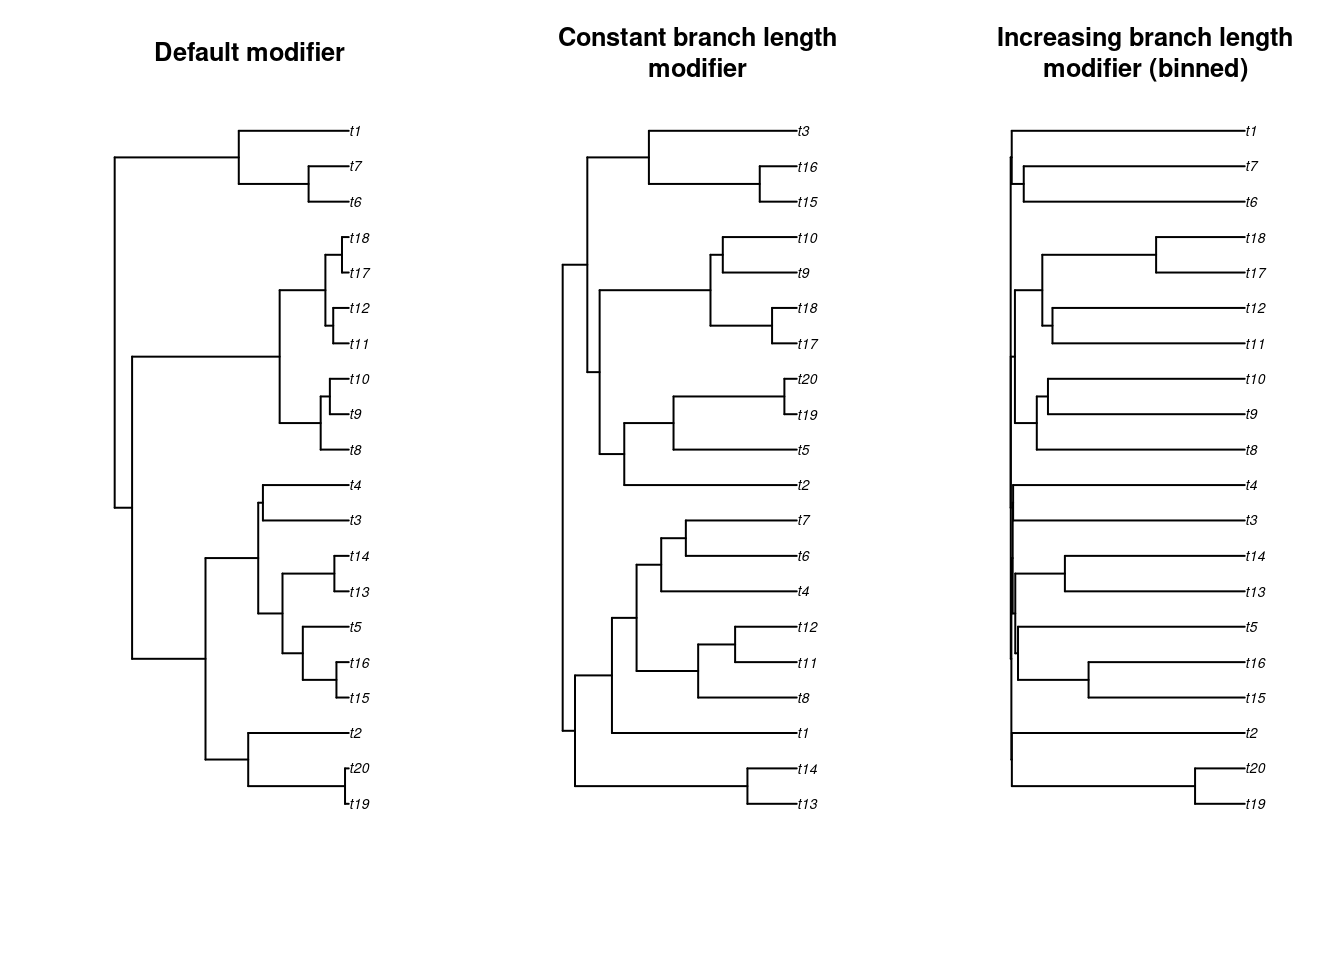
\includegraphics{treats_manual_files/figure-latex/unnamed-chunk-76-1.pdf}

\begin{Shaded}
\begin{Highlighting}[]
\KeywordTok{par}\NormalTok{(}\DataTypeTok{mfrow =} \KeywordTok{c}\NormalTok{(}\DecValTok{1}\NormalTok{,}\DecValTok{1}\NormalTok{))}
\end{Highlighting}
\end{Shaded}

\hypertarget{the-selection-function-selection}{%
\section{\texorpdfstring{The selection function (\texttt{selection})}{The selection function (selection)}}\label{the-selection-function-selection}}

The \texttt{selection} function is used in the birth-death process to know which lineage to select when running a speciation (or extinction!) event.
By default, this function randomly selects one taxon that is currently not extinct (using: \texttt{sample(1:lineage\$n,\ 1))}.
Similarly to \texttt{branch.length}, it is possible to modify this part of the birth-death process.
For example, we could simply select the last created lineage to create a ``ladder'' or most asymmetric tree:

\begin{Shaded}
\begin{Highlighting}[]
\CommentTok{\#\# Our function to always select the last taxon}
\CommentTok{\#\# (making sure it returns an integer)}
\NormalTok{select.last \textless{}{-}}\StringTok{ }\ControlFlowTok{function}\NormalTok{(lineage) \{}
    \KeywordTok{return}\NormalTok{(}\KeywordTok{as.integer}\NormalTok{(lineage}\OperatorTok{$}\NormalTok{n))}
\NormalTok{\}}
\end{Highlighting}
\end{Shaded}

\begin{quote}
Note that here the function can only take the \protect\hyperlink{allowarguments}{allowed arguments as described above} (here \texttt{lineage\$n}: the number of current living taxa).
\end{quote}

We can then create a \texttt{"modifiers"} object the same way as before this time using the \texttt{selection} argument:

\begin{Shaded}
\begin{Highlighting}[]
\CommentTok{\#\# A modifier for selection}
\NormalTok{ladderised\_modifier \textless{}{-}}\StringTok{ }\KeywordTok{make.modifiers}\NormalTok{(}\DataTypeTok{selection =}\NormalTok{ select.last)}
\CommentTok{\#\# Generating a new tree with this modifier}
\KeywordTok{set.seed}\NormalTok{(}\DecValTok{0}\NormalTok{)}
\NormalTok{ladderised\_tree \textless{}{-}}\StringTok{ }\KeywordTok{treats}\NormalTok{(}\DataTypeTok{bd.params =}\NormalTok{ bd\_params,}
                        \DataTypeTok{stop.rule =}\NormalTok{ stop\_rule,}
                        \DataTypeTok{modifiers =}\NormalTok{ ladderised\_modifier)}
\CommentTok{\#\# Displaying the results}
\KeywordTok{par}\NormalTok{(}\DataTypeTok{mfrow =} \KeywordTok{c}\NormalTok{(}\DecValTok{1}\NormalTok{,}\DecValTok{2}\NormalTok{))}
\KeywordTok{plot}\NormalTok{(default\_tree,    }\DataTypeTok{main =} \StringTok{"Default modifier"}\NormalTok{)}
\KeywordTok{plot}\NormalTok{(ladderised\_tree, }\DataTypeTok{main =} \StringTok{"Ladderising modifier"}\NormalTok{)}
\end{Highlighting}
\end{Shaded}

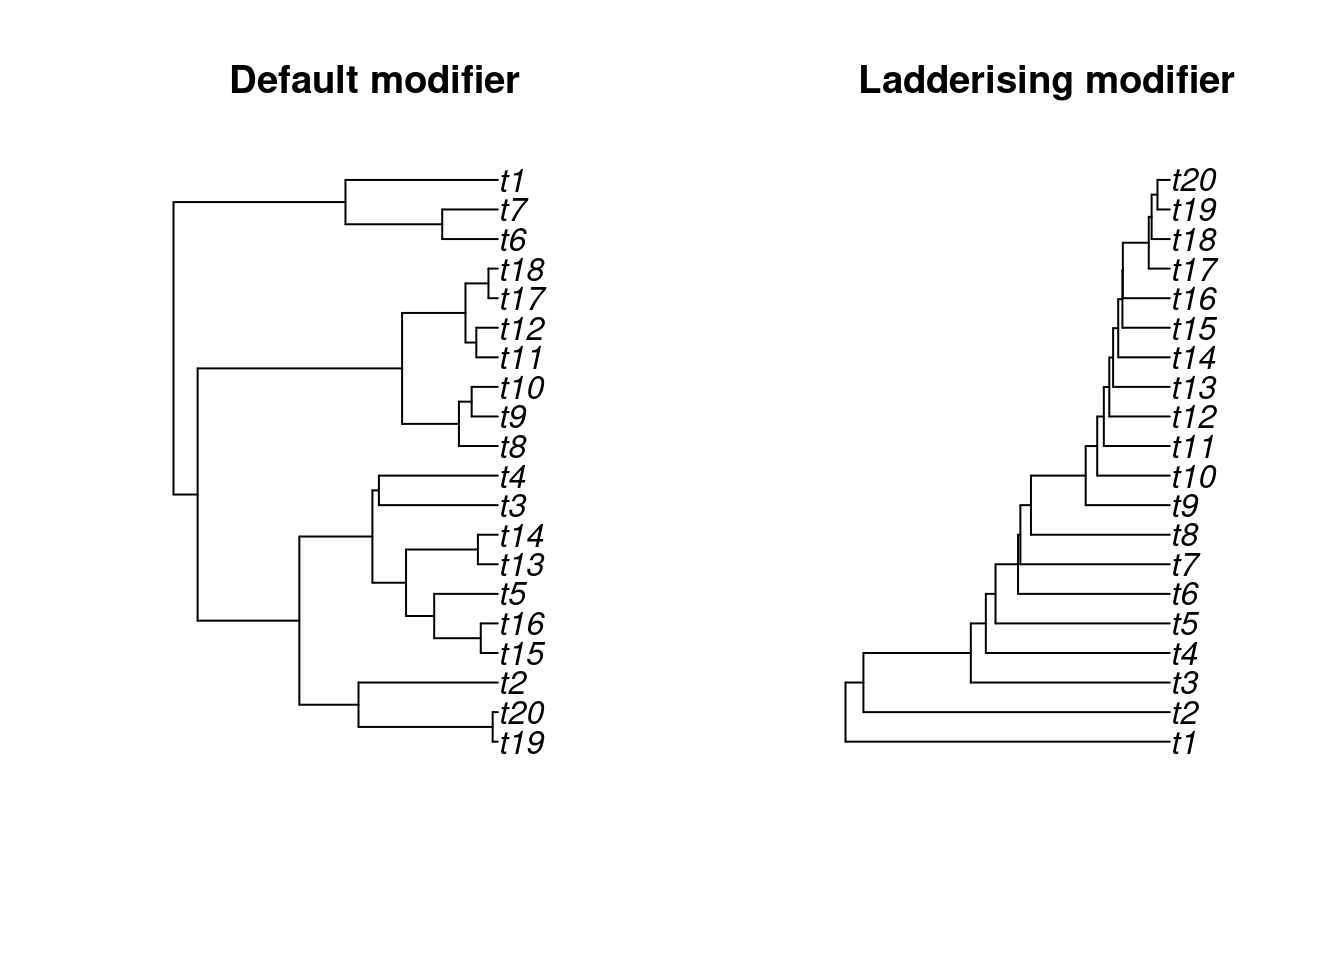
\includegraphics{treats_manual_files/figure-latex/unnamed-chunk-78-1.pdf}

\begin{Shaded}
\begin{Highlighting}[]
\KeywordTok{par}\NormalTok{(}\DataTypeTok{mfrow =} \KeywordTok{c}\NormalTok{(}\DecValTok{1}\NormalTok{,}\DecValTok{1}\NormalTok{))}
\end{Highlighting}
\end{Shaded}

Again, it is of course possible to make the modifier more complex and in combination with other elements of the tree.
For example, we can create a \texttt{"treats"} object that also generates a BM trait and add to it this object a \texttt{selection} modifier that only selects tips with positive trait values (only species with positive trait values will speciate).

\begin{Shaded}
\begin{Highlighting}[]
\CommentTok{\#\# Our function that only select taxa with positive trait values}
\NormalTok{select.positive \textless{}{-}}\StringTok{ }\ControlFlowTok{function}\NormalTok{(trait.values, lineage) \{}

    \CommentTok{\#\# Selecting the taxa names with positive values for the first trait}
\NormalTok{    positives \textless{}{-}}\StringTok{ }\KeywordTok{as.integer}\NormalTok{(}\KeywordTok{rownames}\NormalTok{(trait.values)[}\KeywordTok{which}\NormalTok{(trait.values[, }\DecValTok{1}\NormalTok{] }\OperatorTok{\textgreater{}=}\StringTok{ }\DecValTok{0}\NormalTok{)])}

    \CommentTok{\#\# Combine the descendants of the current lineages (lineage$parents)}
    \CommentTok{\#\# with the species that have speciated (seq\_along(lineages$split))}
    \CommentTok{\#\# to have a table of pairs of parents/splits}
\NormalTok{    parents\_split\_table \textless{}{-}}\StringTok{ }\KeywordTok{cbind}\NormalTok{(lineage}\OperatorTok{$}\NormalTok{parents, }\KeywordTok{seq\_along}\NormalTok{(lineage}\OperatorTok{$}\NormalTok{split))}
    \CommentTok{\#\# Select the current taxa that descend from a node with a positive value}
\NormalTok{    positive\_living \textless{}{-}}\StringTok{ }\NormalTok{parents\_split\_table[}\KeywordTok{which}\NormalTok{(lineage}\OperatorTok{$}\NormalTok{parents }\OperatorTok{\%in\%}\StringTok{ }\NormalTok{positives), }\DecValTok{2}\NormalTok{]}

    \CommentTok{\#\# Select one tip randomly in the ones with descendants with positive values}
    \KeywordTok{return}\NormalTok{(}\KeywordTok{sample}\NormalTok{(}\KeywordTok{which}\NormalTok{(lineage}\OperatorTok{$}\NormalTok{livings }\OperatorTok{\%in\%}\StringTok{ }\NormalTok{positive\_living), }\DecValTok{1}\NormalTok{))}
\NormalTok{\}}

\CommentTok{\#\# Creating the modifier}
\NormalTok{positive\_skew \textless{}{-}}\StringTok{ }\KeywordTok{make.modifiers}\NormalTok{(}\DataTypeTok{selection =}\NormalTok{ select.positive)}

\CommentTok{\#\# Creating a (default) trait object}
\NormalTok{BM\_trait \textless{}{-}}\StringTok{ }\KeywordTok{make.traits}\NormalTok{()}

\CommentTok{\#\# Simulate a tree and trait with no modifier}
\KeywordTok{set.seed}\NormalTok{(}\DecValTok{1}\NormalTok{)}
\NormalTok{default\_treats \textless{}{-}}\StringTok{ }\KeywordTok{treats}\NormalTok{(}\DataTypeTok{bd.params =}\NormalTok{ bd\_params,}
                     \DataTypeTok{stop.rule =}\NormalTok{ stop\_rule,}
                     \DataTypeTok{traits =}\NormalTok{ BM\_trait)}

\CommentTok{\#\# Simulate a tree and trait with the modifier}
\KeywordTok{set.seed}\NormalTok{(}\DecValTok{1}\NormalTok{)}
\NormalTok{skewed\_trait\_treats \textless{}{-}}\StringTok{ }\KeywordTok{treats}\NormalTok{(}\DataTypeTok{bd.params =}\NormalTok{ bd\_params,}
                          \DataTypeTok{stop.rule =}\NormalTok{ stop\_rule,}
                          \DataTypeTok{traits =}\NormalTok{ BM\_trait,}
                          \DataTypeTok{modifiers =}\NormalTok{ positive\_skew)}

\CommentTok{\#\# Plotting the differences in trees and traits}
\KeywordTok{par}\NormalTok{(}\DataTypeTok{mfrow =} \KeywordTok{c}\NormalTok{(}\DecValTok{1}\NormalTok{, }\DecValTok{2}\NormalTok{))}
\KeywordTok{plot}\NormalTok{(default\_treats, }\DataTypeTok{main =} \StringTok{"Default trait and tree"}\NormalTok{)}
\KeywordTok{plot}\NormalTok{(skewed\_trait\_treats, }\DataTypeTok{main =} \StringTok{"Skewed trait and tree"}\NormalTok{)}
\end{Highlighting}
\end{Shaded}

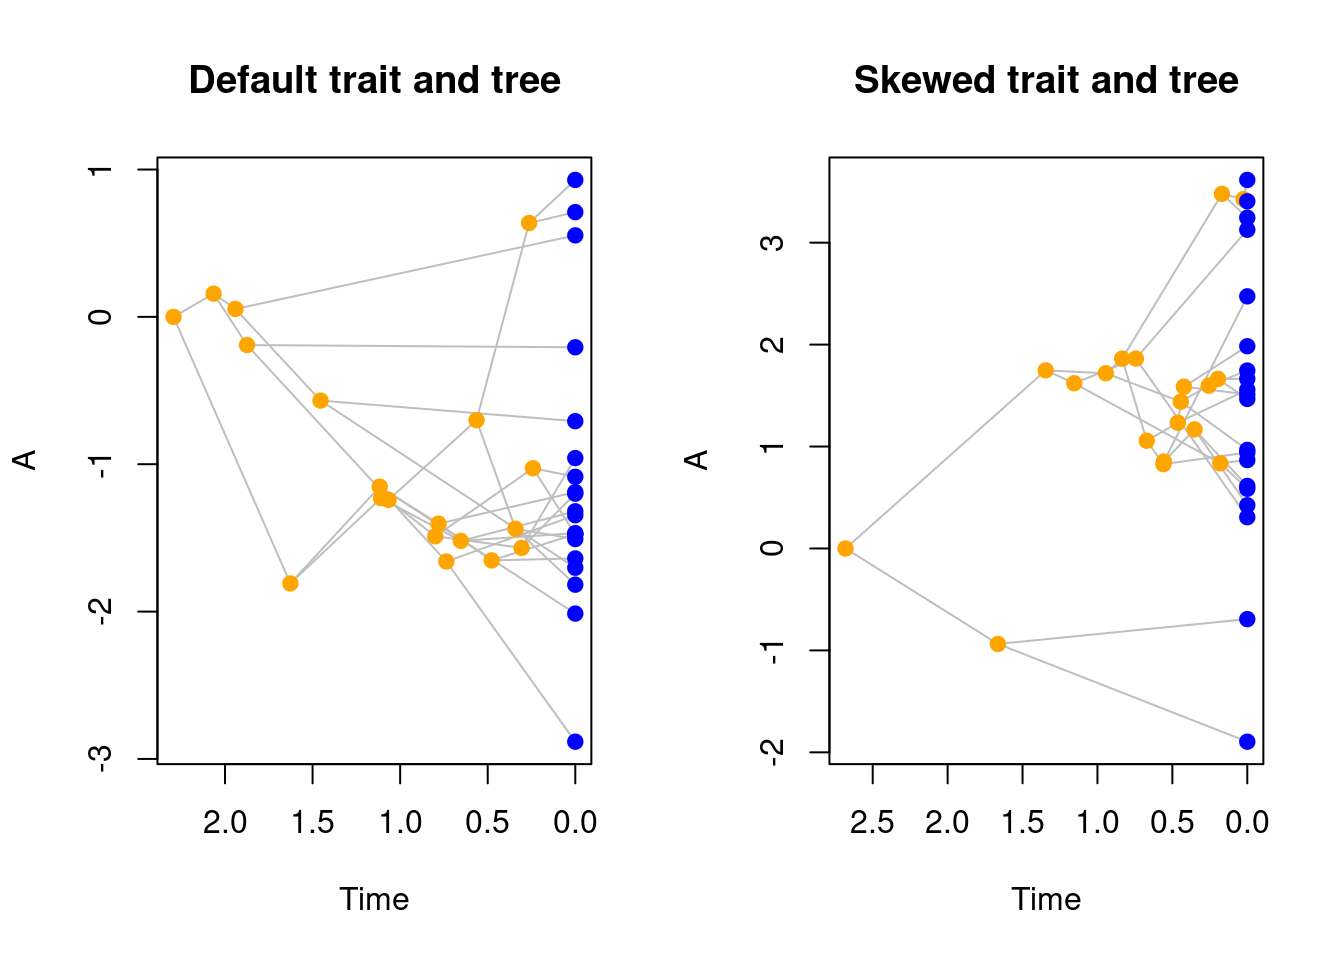
\includegraphics{treats_manual_files/figure-latex/unnamed-chunk-79-1.pdf}

\hypertarget{the-speciation-function-speciation}{%
\section{\texorpdfstring{The speciation function (\texttt{speciation})}{The speciation function (speciation)}}\label{the-speciation-function-speciation}}

The third function that can be used to modify the birth-death process is the \texttt{speciation} function.
This one is used during the birth-death process to decide whether a lineage speciates (creating a node and two new lineages) or goes extinct (creating a tip).

\begin{quote}
Note that the \texttt{speciation} function only affects tips or nodes before the simulation reaches the \texttt{stop.rule}.
The then surviving lineages are all automatically transformed into tips.
\end{quote}

By default, the \texttt{speciation} function is trigger a speciation even if a number randomly drawn from a uniform distribution is lower than the ratio between the speciation and the speciation and extinction parameter. If the randomly drawn number is higher, the lineage goes extinct.

\begin{Shaded}
\begin{Highlighting}[]
\CommentTok{\#\# The speciation in pseudo{-}code:}
\KeywordTok{runif}\NormalTok{(}\DecValTok{1}\NormalTok{) }\OperatorTok{\textless{}}\StringTok{ }\NormalTok{speciation}\OperatorTok{/}\StringTok{ }\NormalTok{(speciation }\OperatorTok{+}\StringTok{ }\NormalTok{extinction)}
\end{Highlighting}
\end{Shaded}

Creating \texttt{"modifiers"} with a \texttt{speciation} function works the same way as for \texttt{branch.length} and \texttt{selection} but the function that will be used needs to output a logical value (see table \protect\hyperlink{summarymodifiers}{below}).
Once the function is created simply input your function for speciation in the modifier and run the \texttt{treats} function with that modifier:

\begin{Shaded}
\begin{Highlighting}[]
\CommentTok{\#\# Speciating or going extinct randomly}
\CommentTok{\#\# (regardless of the extinction parameter)}
\NormalTok{random.extinct  \textless{}{-}}\StringTok{ }\ControlFlowTok{function}\NormalTok{() \{}
    \KeywordTok{return}\NormalTok{(}\KeywordTok{sample}\NormalTok{(}\KeywordTok{c}\NormalTok{(}\OtherTok{TRUE}\NormalTok{, }\OtherTok{FALSE}\NormalTok{), }\DecValTok{1}\NormalTok{))}
\NormalTok{\}}

\CommentTok{\#\# Creating the modifiers object}
\NormalTok{random\_extinction \textless{}{-}}\StringTok{ }\KeywordTok{make.modifiers}\NormalTok{(}\DataTypeTok{speciation =}\NormalTok{ random.extinct)}

\CommentTok{\#\# Generating a new tree with this modifier}
\KeywordTok{set.seed}\NormalTok{(}\DecValTok{2}\NormalTok{)}
\NormalTok{modified\_tree \textless{}{-}}\StringTok{ }\KeywordTok{treats}\NormalTok{(}\DataTypeTok{bd.params =}\NormalTok{ bd\_params,}
                      \DataTypeTok{stop.rule =}\NormalTok{ stop\_rule,}
                      \DataTypeTok{modifiers =}\NormalTok{ random\_extinction)}

\KeywordTok{par}\NormalTok{(}\DataTypeTok{mfrow =} \KeywordTok{c}\NormalTok{(}\DecValTok{1}\NormalTok{,}\DecValTok{2}\NormalTok{))}
\KeywordTok{plot}\NormalTok{(default\_tree,  }\DataTypeTok{main =} \StringTok{"Default modifier"}\NormalTok{)}
\KeywordTok{plot}\NormalTok{(modified\_tree, }\DataTypeTok{main =} \StringTok{"Random extinction}\CharTok{\textbackslash{}n}\StringTok{modifier"}\NormalTok{)}
\KeywordTok{par}\NormalTok{(}\DataTypeTok{mfrow =} \KeywordTok{c}\NormalTok{(}\DecValTok{1}\NormalTok{,}\DecValTok{1}\NormalTok{))}
\end{Highlighting}
\end{Shaded}

\begin{quote}
Note how loads of lineages go extinct even if the extinction parameter is set to 0!
\end{quote}

And again, we can make some more advanced modifiers: for example, one where a tip always goes extinct if their ancestor has a negative trait value. Here we will also introduce the utility function \texttt{parent.trait} that automatically selects the trait values of the parent of the current lineage.

\begin{Shaded}
\begin{Highlighting}[]
\CommentTok{\#\# A modifier for removing tips with negative values}
\NormalTok{modify.trait \textless{}{-}}\StringTok{ }\ControlFlowTok{function}\NormalTok{(trait.values, lineage) \{}
    \ControlFlowTok{if}\NormalTok{(}\KeywordTok{parent.traits}\NormalTok{(trait.values, lineage) }\OperatorTok{\textless{}}\StringTok{ }\DecValTok{0}\NormalTok{) \{}
        \CommentTok{\#\# Go extinct!}
        \KeywordTok{return}\NormalTok{(}\OtherTok{FALSE}\NormalTok{)}
\NormalTok{    \} }\ControlFlowTok{else}\NormalTok{ \{}
        \CommentTok{\#\# Speciate!}
        \KeywordTok{return}\NormalTok{(}\OtherTok{TRUE}\NormalTok{)}
\NormalTok{    \}}
\NormalTok{\}}

\CommentTok{\#\# Creating the modifier}
\NormalTok{modified\_trait \textless{}{-}}\StringTok{ }\KeywordTok{make.modifiers}\NormalTok{(}\DataTypeTok{speciation =}\NormalTok{ modify.trait)}

\CommentTok{\#\# Simulate a tree and trait with the modifier}
\KeywordTok{set.seed}\NormalTok{(}\DecValTok{1}\NormalTok{)}
\NormalTok{modified\_trait\_treats \textless{}{-}}\StringTok{ }\KeywordTok{treats}\NormalTok{(}\DataTypeTok{bd.params =}\NormalTok{ bd\_params,}
                          \DataTypeTok{stop.rule =}\NormalTok{ stop\_rule,}
                          \DataTypeTok{traits    =}\NormalTok{ BM\_trait,}
                          \DataTypeTok{modifiers =}\NormalTok{ modified\_trait)}

\CommentTok{\#\# Plotting the differences in trees and traits}
\KeywordTok{par}\NormalTok{(}\DataTypeTok{mfrow =} \KeywordTok{c}\NormalTok{(}\DecValTok{1}\NormalTok{, }\DecValTok{2}\NormalTok{))}
\KeywordTok{plot}\NormalTok{(default\_treats, }\DataTypeTok{main =} \StringTok{"Default trait and tree"}\NormalTok{)}
\KeywordTok{plot}\NormalTok{(modified\_trait\_treats, }\DataTypeTok{main =} \StringTok{"Biased trait and tree"}\NormalTok{)}
\end{Highlighting}
\end{Shaded}

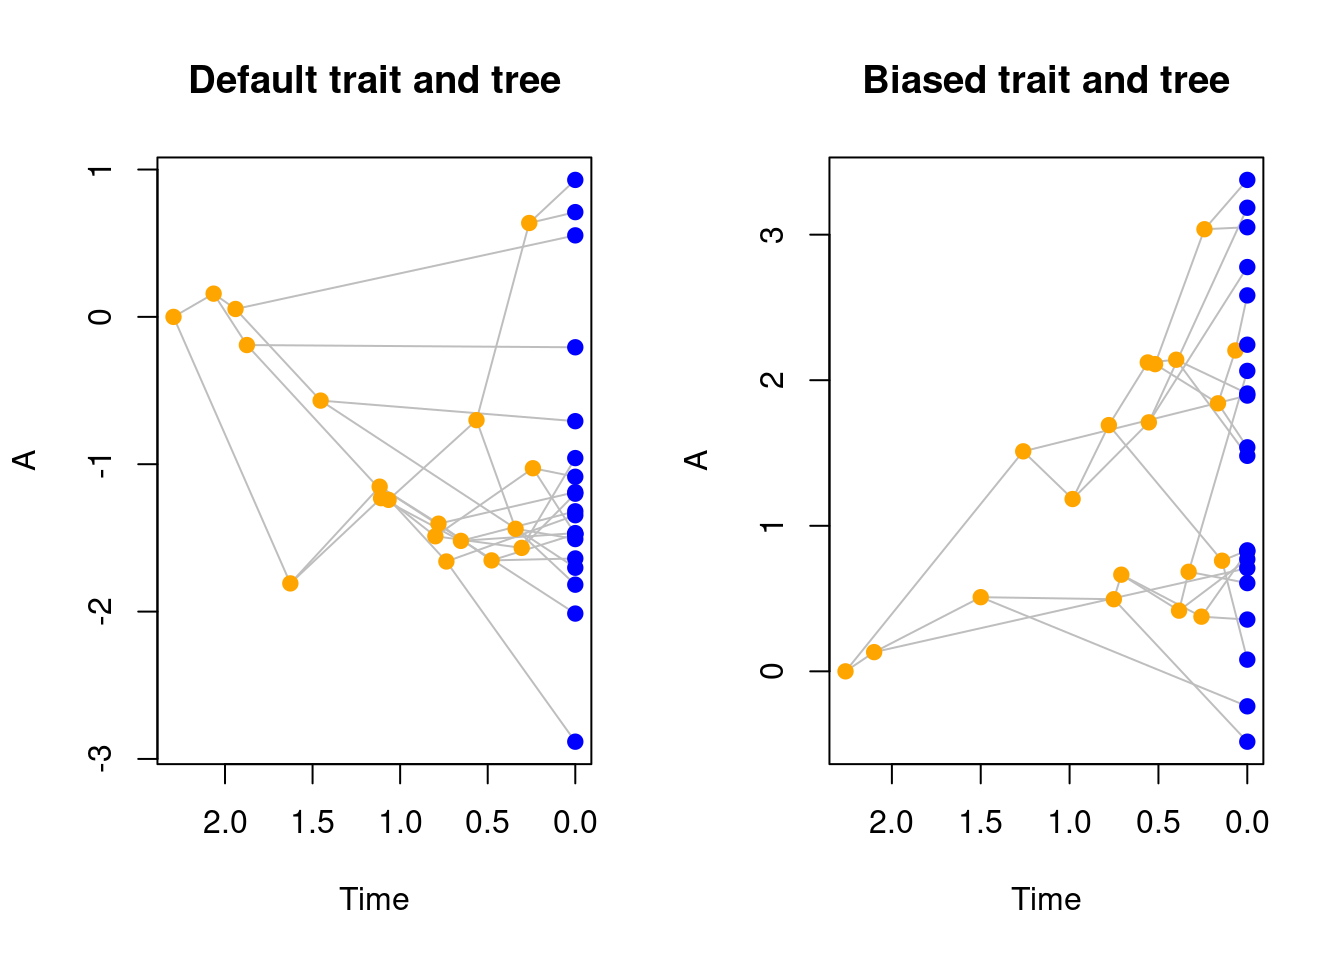
\includegraphics{treats_manual_files/figure-latex/unnamed-chunk-82-1.pdf}

\hypertarget{summarymodifiers}{%
\section{\texorpdfstring{Summary of the inputs and outputs for the \texttt{branch.length}, \texttt{selection} and \texttt{speciation} modifiers}{Summary of the inputs and outputs for the branch.length, selection and speciation modifiers}}\label{summarymodifiers}}

\begin{longtable}[]{@{}lll@{}}
\toprule
modifier name & accepted input (arguments) & required output (class)\tabularnewline
\midrule
\endhead
\texttt{branch.length} & \texttt{bd.params}, \texttt{lineage}, \texttt{trait.values} & \texttt{"numeric"}\tabularnewline
\texttt{selection} & \texttt{bd.params}, \texttt{lineage}, \texttt{trait.values} & \texttt{"integer"}\tabularnewline
\texttt{speciation} & \texttt{bd.params}, \texttt{lineage}, \texttt{trait.values} & \texttt{"logical"}\tabularnewline
\bottomrule
\end{longtable}

\hypertarget{the-condition-and-modify-functions-condition-and-modify}{%
\section{\texorpdfstring{The condition and modify functions (\texttt{condition} and \texttt{modify})}{The condition and modify functions (condition and modify)}}\label{the-condition-and-modify-functions-condition-and-modify}}

In the examples above, we have seen how to specify modifications to the birth-death process (via \texttt{branch.length}, \texttt{selection} and \texttt{speciation}), however, these modifications are not dynamic.
In other words, throughout the process, the modifications remain constant (even if they are conditional).
It is however, possible to code the \texttt{"modifiers"} so that they can be affected by \texttt{"events"} objects (see next chapter \protect\hyperlink{makeevents}{on \texttt{events}}).

To do so, you can formally declare conditions (\texttt{condition}) and modifications (\texttt{modify}) as internal functions that can then be modified by an \texttt{"events"} object.
\texttt{condition} and \texttt{modify} are hard coded in the \texttt{branch.length} function that they concern, i.e.~they are variables (functions) within the function.

For example in the \texttt{speciation} part of a modifier, the default is to trigger an event from a uniform distribution and then check if that value is smaller than (\(speciation/(speciation + extinction)\)):

\begin{Shaded}
\begin{Highlighting}[]
\CommentTok{\#\# The default speciation algorithm}
\NormalTok{speciation \textless{}{-}}\StringTok{ }\ControlFlowTok{function}\NormalTok{(bd.params) \{}
    \CommentTok{\#\# Randomly trigger an event}
\NormalTok{    trigger\_event \textless{}{-}}\StringTok{ }\KeywordTok{runif}\NormalTok{(}\DecValTok{1}\NormalTok{)}

    \CommentTok{\#\# Speciate?}
    \KeywordTok{return}\NormalTok{(trigger\_event }\OperatorTok{\textless{}}\StringTok{ }\NormalTok{(bd.params}\OperatorTok{$}\NormalTok{speciation}\OperatorTok{/}
\StringTok{                              }\NormalTok{(bd.params}\OperatorTok{$}\NormalTok{speciation }\OperatorTok{+}\StringTok{ }\NormalTok{bd.params}\OperatorTok{$}\NormalTok{extinction)))}
\NormalTok{\}}
\end{Highlighting}
\end{Shaded}

It is possible with some specific conditions to modify this trigger by providing a \texttt{condition} and \texttt{modify} function to the speciation function.
That is, if the \texttt{condition} is met, apply the \texttt{modify} function to the algorithm.
For example here we can edit the default speciation function to have a modification (\texttt{modify\ =\ double.the.trigger}: doubling the trigger value) happening half the time (\texttt{condition\ =\ half.the.time}):

\begin{Shaded}
\begin{Highlighting}[]
\CommentTok{\#\# A conditional function that triggers half the time}
\NormalTok{half.the.time \textless{}{-}}\StringTok{ }\ControlFlowTok{function}\NormalTok{() }\KeywordTok{return}\NormalTok{(}\KeywordTok{sample}\NormalTok{(}\KeywordTok{c}\NormalTok{(}\OtherTok{TRUE}\NormalTok{, }\OtherTok{FALSE}\NormalTok{), }\DecValTok{1}\NormalTok{))}
\CommentTok{\#\# A modification that doubles the value to trigger the event}
\NormalTok{double.the.trigger \textless{}{-}}\StringTok{ }\ControlFlowTok{function}\NormalTok{(x) }\KeywordTok{return}\NormalTok{(x}\OperatorTok{*}\DecValTok{2}\NormalTok{)}
\CommentTok{\#\# A conditional modifier}
\KeywordTok{make.modifiers}\NormalTok{(}\DataTypeTok{speciation =}\NormalTok{ speciation,}
               \DataTypeTok{condition  =}\NormalTok{ half.the.time, }
               \DataTypeTok{modify =}\NormalTok{ double.the.trigger)}
\end{Highlighting}
\end{Shaded}

\begin{verbatim}
##  ---- treats modifiers object ---- 
## Default branch length process.
## Default selection process.
## Speciation process is set to speciation with a condition (half.the.time) and a modifier (double.the.trigger).
\end{verbatim}

Effectively, this will internally modify the speciation function as follows:

\begin{Shaded}
\begin{Highlighting}[]
\CommentTok{\#\# The default speciation algorithm}
\NormalTok{speciation \textless{}{-}}\StringTok{ }\ControlFlowTok{function}\NormalTok{(bd.params) \{}
    \CommentTok{\#\# Randomly trigger an event}
\NormalTok{    trigger\_event \textless{}{-}}\StringTok{ }\KeywordTok{runif}\NormalTok{(}\DecValTok{1}\NormalTok{)}

    \CommentTok{\#\# Modify the triggering}
    \ControlFlowTok{if}\NormalTok{(}\KeywordTok{half.the.time}\NormalTok{()) \{ }\CommentTok{\#\# This running the half.the.time function drawing TRUE or FALSE randomly}
\NormalTok{        trigger\_event \textless{}{-}}\StringTok{ }\KeywordTok{double.the.trigger}\NormalTok{(trigger\_event) }\CommentTok{\#\# This will double the random value trigger\_event}
\NormalTok{    \}}

    \CommentTok{\#\# Speciate?}
    \KeywordTok{return}\NormalTok{(trigger\_event }\OperatorTok{\textless{}}\StringTok{ }\NormalTok{(bd.params}\OperatorTok{$}\NormalTok{speciation}\OperatorTok{/}
\StringTok{                              }\NormalTok{(bd.params}\OperatorTok{$}\NormalTok{speciation }\OperatorTok{+}\StringTok{ }\NormalTok{bd.params}\OperatorTok{$}\NormalTok{extinction)))}
\NormalTok{\}}
\end{Highlighting}
\end{Shaded}

These \texttt{condition} and \texttt{modify} functions can be applied to all the \texttt{modifiers} elements (\texttt{selection}, \texttt{branch.length} and \texttt{speciation}).
However, they are typically used in \texttt{events} that will modify the \texttt{modifiers} (\protect\hyperlink{makeevents}{see the \texttt{events} section})!

\begin{verbatim}
## This build of rgl does not include OpenGL functions.  Use
##  rglwidget() to display results, e.g. via options(rgl.printRglwidget = TRUE).
\end{verbatim}

\hypertarget{makeevents}{%
\chapter{Adding events to simulations}\label{makeevents}}

One other major feature of the \texttt{treats} package is that it allows simulations to run with specified events that occur during the simulation.
These are typically events that can drastically change the course of the simulation.
For example, you might want simulate a mass extinction at some specific point in time.
However, these can also be more subtle, like the internal change of parameter values when reaching a specific trait value.
These are all handled by \texttt{treats} with the \texttt{events} object that you can create using \texttt{make.events} and has the same overall logic as \texttt{make.traits} and \texttt{make.modifiers}.

\texttt{events} require three main arguments:
* the \texttt{target} which designates what the extinction should affect (e.g.~the taxa, the speciation rate, etc\ldots);
* the \texttt{condition} which designates when to trigger the event;
* the \texttt{modification} which designates what to modify when the event is triggered.

There are several more arguments that can be passed to \texttt{make.events} but they are discussed later on.
First let's focus on these three main arguments:

\begin{figure}
\centering
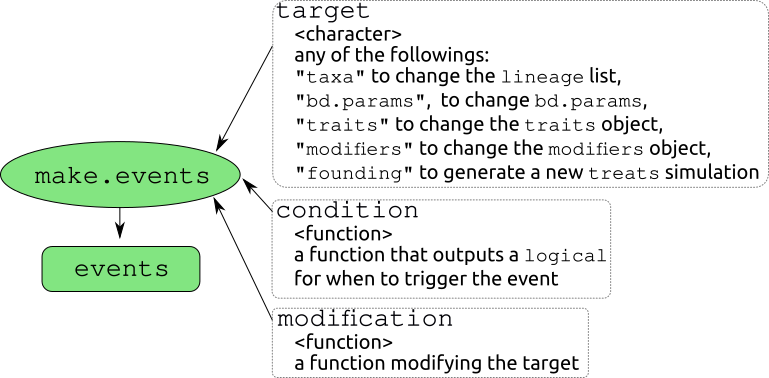
\includegraphics{make.events.png}
\caption{\texttt{make.events}: events are encoded using three main arguments: the \texttt{target}, specifying \emph{what} the event is modifying, the \texttt{condition} specifying \emph{when} to trigger the event, and \texttt{modification}, specifying \emph{how} the event modifies the simulations.}
\end{figure}

\hypertarget{quick-overview-2}{%
\subsection{Quick overview}\label{quick-overview-2}}

condition,
modification,
add,
test = TRUE,
event.name,
replications = 0,
additional.args
)

\begin{longtable}[]{@{}llll@{}}
\toprule
\begin{minipage}[b]{0.19\columnwidth}\raggedright
function\strut
\end{minipage} & \begin{minipage}[b]{0.23\columnwidth}\raggedright
arguments\strut
\end{minipage} & \begin{minipage}[b]{0.14\columnwidth}\raggedright
input\strut
\end{minipage} & \begin{minipage}[b]{0.33\columnwidth}\raggedright
what does it do\strut
\end{minipage}\tabularnewline
\midrule
\endhead
\begin{minipage}[t]{0.19\columnwidth}\raggedright
\texttt{make.events}\strut
\end{minipage} & \begin{minipage}[t]{0.23\columnwidth}\raggedright
target*\strut
\end{minipage} & \begin{minipage}[t]{0.14\columnwidth}\raggedright
any of the following: ``taxa'', ``bd.params'', ``traits'', ``modifiers'' or ``founding''\strut
\end{minipage} & \begin{minipage}[t]{0.33\columnwidth}\raggedright
what aspect of the simulation should the event target\strut
\end{minipage}\tabularnewline
\begin{minipage}[t]{0.19\columnwidth}\raggedright
\texttt{make.events}\strut
\end{minipage} & \begin{minipage}[t]{0.23\columnwidth}\raggedright
condition*\strut
\end{minipage} & \begin{minipage}[t]{0.14\columnwidth}\raggedright
a function\strut
\end{minipage} & \begin{minipage}[t]{0.33\columnwidth}\raggedright
a function that affects the condition of when to trigger the event (see below)\strut
\end{minipage}\tabularnewline
\begin{minipage}[t]{0.19\columnwidth}\raggedright
\texttt{make.events}\strut
\end{minipage} & \begin{minipage}[t]{0.23\columnwidth}\raggedright
modification*\strut
\end{minipage} & \begin{minipage}[t]{0.14\columnwidth}\raggedright
a function\strut
\end{minipage} & \begin{minipage}[t]{0.33\columnwidth}\raggedright
a function that applies the modification to the target if the condition is triggered (see below)\strut
\end{minipage}\tabularnewline
\begin{minipage}[t]{0.19\columnwidth}\raggedright
\texttt{make.events}\strut
\end{minipage} & \begin{minipage}[t]{0.23\columnwidth}\raggedright
add\strut
\end{minipage} & \begin{minipage}[t]{0.14\columnwidth}\raggedright
a \texttt{treats} object\strut
\end{minipage} & \begin{minipage}[t]{0.33\columnwidth}\raggedright
another event generated by \texttt{make.events}\strut
\end{minipage}\tabularnewline
\begin{minipage}[t]{0.19\columnwidth}\raggedright
\texttt{make.events}\strut
\end{minipage} & \begin{minipage}[t]{0.23\columnwidth}\raggedright
test\strut
\end{minipage} & \begin{minipage}[t]{0.14\columnwidth}\raggedright
logical\strut
\end{minipage} & \begin{minipage}[t]{0.33\columnwidth}\raggedright
whether to test the validity of the event\strut
\end{minipage}\tabularnewline
\begin{minipage}[t]{0.19\columnwidth}\raggedright
\texttt{make.events}\strut
\end{minipage} & \begin{minipage}[t]{0.23\columnwidth}\raggedright
event.name\strut
\end{minipage} & \begin{minipage}[t]{0.14\columnwidth}\raggedright
a character string\strut
\end{minipage} & \begin{minipage}[t]{0.33\columnwidth}\raggedright
the name of the event\strut
\end{minipage}\tabularnewline
\begin{minipage}[t]{0.19\columnwidth}\raggedright
\texttt{make.events}\strut
\end{minipage} & \begin{minipage}[t]{0.23\columnwidth}\raggedright
replications\strut
\end{minipage} & \begin{minipage}[t]{0.14\columnwidth}\raggedright
a number\strut
\end{minipage} & \begin{minipage}[t]{0.33\columnwidth}\raggedright
if possible how many times is the event allowing to be repeated\strut
\end{minipage}\tabularnewline
\begin{minipage}[t]{0.19\columnwidth}\raggedright
\texttt{make.events}\strut
\end{minipage} & \begin{minipage}[t]{0.23\columnwidth}\raggedright
additional.args\strut
\end{minipage} & \begin{minipage}[t]{0.14\columnwidth}\raggedright
\ldots{}\strut
\end{minipage} & \begin{minipage}[t]{0.33\columnwidth}\raggedright
any additional arguments to be passed to the event\strut
\end{minipage}\tabularnewline
\bottomrule
\end{longtable}

Here is a list of implemented \texttt{conditions} (see \texttt{?events.conditions}):

\begin{longtable}[]{@{}llll@{}}
\toprule
\begin{minipage}[b]{0.19\columnwidth}\raggedright
function\strut
\end{minipage} & \begin{minipage}[b]{0.23\columnwidth}\raggedright
arguments\strut
\end{minipage} & \begin{minipage}[b]{0.14\columnwidth}\raggedright
input\strut
\end{minipage} & \begin{minipage}[b]{0.33\columnwidth}\raggedright
what does it do\strut
\end{minipage}\tabularnewline
\midrule
\endhead
\begin{minipage}[t]{0.19\columnwidth}\raggedright
\texttt{age.condition}, \texttt{taxa.condition}, \texttt{trait.condition}\strut
\end{minipage} & \begin{minipage}[t]{0.23\columnwidth}\raggedright
x\strut
\end{minipage} & \begin{minipage}[t]{0.14\columnwidth}\raggedright
the value to check the target against\strut
\end{minipage} & \begin{minipage}[t]{0.33\columnwidth}\raggedright
e.g.~time = x, taxa = x or trait = x (see below)\strut
\end{minipage}\tabularnewline
\begin{minipage}[t]{0.19\columnwidth}\raggedright
\ldots{}\strut
\end{minipage} & \begin{minipage}[t]{0.23\columnwidth}\raggedright
condition\strut
\end{minipage} & \begin{minipage}[t]{0.14\columnwidth}\raggedright
a relational operator\strut
\end{minipage} & \begin{minipage}[t]{0.33\columnwidth}\raggedright
e.g.~\texttt{==}, \texttt{\textgreater{}}, \texttt{!=}, etc. for asking for example \texttt{time\ ==\ x}\strut
\end{minipage}\tabularnewline
\begin{minipage}[t]{0.19\columnwidth}\raggedright
\ldots{}\strut
\end{minipage} & \begin{minipage}[t]{0.23\columnwidth}\raggedright
\ldots{}\strut
\end{minipage} & \begin{minipage}[t]{0.14\columnwidth}\raggedright
any additional arguments to be passed to the event\strut
\end{minipage} & \begin{minipage}[t]{0.33\columnwidth}\raggedright
\strut
\end{minipage}\tabularnewline
\bottomrule
\end{longtable}

Here is a list of implemented \texttt{modifications} (see \texttt{?events.modifications}):

\begin{longtable}[]{@{}llll@{}}
\toprule
\begin{minipage}[b]{0.19\columnwidth}\raggedright
function\strut
\end{minipage} & \begin{minipage}[b]{0.23\columnwidth}\raggedright
arguments\strut
\end{minipage} & \begin{minipage}[b]{0.14\columnwidth}\raggedright
input\strut
\end{minipage} & \begin{minipage}[b]{0.33\columnwidth}\raggedright
what does it do\strut
\end{minipage}\tabularnewline
\midrule
\endhead
\begin{minipage}[t]{0.19\columnwidth}\raggedright
\texttt{random.extinction}\strut
\end{minipage} & \begin{minipage}[t]{0.23\columnwidth}\raggedright
x\strut
\end{minipage} & \begin{minipage}[t]{0.14\columnwidth}\raggedright
a numeric value\strut
\end{minipage} & \begin{minipage}[t]{0.33\columnwidth}\raggedright
the proportion of species to make extinct\strut
\end{minipage}\tabularnewline
\begin{minipage}[t]{0.19\columnwidth}\raggedright
\texttt{trait.extinction}\strut
\end{minipage} & \begin{minipage}[t]{0.23\columnwidth}\raggedright
x\strut
\end{minipage} & \begin{minipage}[t]{0.14\columnwidth}\raggedright
a numeric value\strut
\end{minipage} & \begin{minipage}[t]{0.33\columnwidth}\raggedright
the trait value when to trigger the extinction\strut
\end{minipage}\tabularnewline
\begin{minipage}[t]{0.19\columnwidth}\raggedright
\texttt{trait.extinction}\strut
\end{minipage} & \begin{minipage}[t]{0.23\columnwidth}\raggedright
condition\strut
\end{minipage} & \begin{minipage}[t]{0.14\columnwidth}\raggedright
a relational operator\strut
\end{minipage} & \begin{minipage}[t]{0.33\columnwidth}\raggedright
the relation to the trait value (e.g.~\texttt{x\ =\ 1} and \texttt{condition\ =\ \ \textgreater{}} makes species that have a trait value \textgreater{} 1 go extinct)\strut
\end{minipage}\tabularnewline
\begin{minipage}[t]{0.19\columnwidth}\raggedright
\texttt{bd.params.update}\strut
\end{minipage} & \begin{minipage}[t]{0.23\columnwidth}\raggedright
\ldots{}\strut
\end{minipage} & \begin{minipage}[t]{0.14\columnwidth}\raggedright
any argument to be passed to \texttt{make.bd.params}\strut
\end{minipage} & \begin{minipage}[t]{0.33\columnwidth}\raggedright
\strut
\end{minipage}\tabularnewline
\begin{minipage}[t]{0.19\columnwidth}\raggedright
\texttt{traits.update}\strut
\end{minipage} & \begin{minipage}[t]{0.23\columnwidth}\raggedright
\ldots{}\strut
\end{minipage} & \begin{minipage}[t]{0.14\columnwidth}\raggedright
any argument to be passed to \texttt{make.traits}\strut
\end{minipage} & \begin{minipage}[t]{0.33\columnwidth}\raggedright
\strut
\end{minipage}\tabularnewline
\begin{minipage}[t]{0.19\columnwidth}\raggedright
\texttt{modifiers.update}\strut
\end{minipage} & \begin{minipage}[t]{0.23\columnwidth}\raggedright
\ldots{}\strut
\end{minipage} & \begin{minipage}[t]{0.14\columnwidth}\raggedright
any argument to be passed to \texttt{make.modifiers}\strut
\end{minipage} & \begin{minipage}[t]{0.33\columnwidth}\raggedright
\strut
\end{minipage}\tabularnewline
\bottomrule
\end{longtable}

* non-optional arguments

\hypertarget{target}{%
\section{Target}\label{target}}

The target of the event is what the event is going to modify in the birth-death algorithm.
You can only have one target per event (along with one condition and one modification) but you can create events that contain multiple events (i.e.~multiple triplets of target/condition/modification).
The targets that are currently available are:

\begin{itemize}
\tightlist
\item
  \texttt{"taxa"} to modify anything linked to the \protect\hyperlink{allowarguments}{\texttt{lineage} list}. e.g.~making half of the living taxa go extinct.
\item
  \texttt{"bd.params"} to modify anything linked to the \protect\hyperlink{makebdparams}{\texttt{bd.params} object}. For example you might want to change the distribution of one of the parameter after some \texttt{conditions}. This is typically done by updating the object using the argument \texttt{update} from \texttt{make.bd.params}.
\item
  \texttt{"traits"} to modify anything linked to the \protect\hyperlink{maketraits}{\texttt{traits} object}. For example you might want to change the trait process after some \texttt{conditions}. This is typically done by updating the object using the argument \texttt{update} from \texttt{make.traits}.
\item
  \texttt{"modifiers"} to modify anything linked to the \protect\hyperlink{makebdmodifiers}{\texttt{modifiers} object}. For example you might want to change the speciation rule after some \texttt{conditions}. This is typically done by updating the object using the argument \texttt{update} from \texttt{make.modifiers}.
\item
  \texttt{"founding"} this target is a bit more specialised and allows you run a nested \texttt{treats} object in the simulation. It is covered in a \protect\hyperlink{founding}{specific section below}.
\end{itemize}

We will see some examples of these targets in the \texttt{conditions} and \texttt{modifications} described below.

\hypertarget{conditions}{%
\section{Conditions}\label{conditions}}

\texttt{condition} is a function that returns a logical value. When a specific condition is met, it should return \texttt{TRUE} and trigger the event, else it should return \texttt{FALSE}.

Currently there are three conditions functions implemented in \texttt{treats} but you can easily come up with your own version of them.

All \texttt{condition} functions in \texttt{treats} take at least two arguments: \texttt{x} for the variable of interest (e.g.~time, number of taxa, trait value, etc.) and \texttt{condition}, the relational operator to evaluate. A relational operator is the proper (fancy) term designating all the comparisons you're regularly using in \texttt{R} like \texttt{==} (is equal?) \texttt{\textless{}} (is smaller?) \texttt{\textgreater{}=} (is bigger or equal?). You can get the full list in the R base manual (using \texttt{?Comparison} or any of the relational operator in a function form). For more details on how functions \emph{really} work in R see the \href{https://adv-r.hadley.nz/functions.html}{Advanced \texttt{R} book}!

\begin{itemize}
\tightlist
\item
  \texttt{age.condition} will trigger the \texttt{event} once a certain time is reached in the simulations and is the simplest/most basic condition with no arguments other than the time required. For example \texttt{age.condition(4,\ condition\ =\ \textasciigrave{}==\textasciigrave{})} will trigger the \texttt{event} once the simulations reaches 4 time units. Easy.
\item
  \texttt{taxa.condition} will trigger the \texttt{event} once a certain number of taxa are reached. This can be considered including or excluding fossil species. For example \texttt{taxa.condition(42,\ condition\ =\ \textasciigrave{}\textgreater{}=\textasciigrave{},\ living\ =\ TRUE)} will trigger the \texttt{event} if there are at least 42 living taxa.
\item
  \texttt{trait.condition} will trigger the \texttt{event} once a certain trait value is reached. This function allows to say which trait(s) to target (by default, the first one using \texttt{trait\ =\ 1}), what value of the trait to target (by default \texttt{what\ =\ max}) and whether to use and absolute trait value or not (\texttt{absolute\ =\ TRUE}). For example \texttt{trait.condition(1/3,\ condition\ =\ \textasciigrave{}\textgreater{}\textasciigrave{},\ trait\ =\ 1,\ what\ =\ sd)} will trigger the condition after the standard deviation of the first trait reaches 1/3.
\end{itemize}

\hypertarget{modifications}{%
\section{Modifications}\label{modifications}}

After defining the \texttt{event}, \texttt{target} and \texttt{condition}, you also need to specify what it should modify.
These are functions that should modify a specific aspect of the target.
Depending on the target you can modify the following:

\begin{itemize}
\tightlist
\item
  if the target is \texttt{"taxa"} you can modify the internal \protect\hyperlink{allowarguments}{\texttt{lineage} list} by removing living species using \texttt{random.extinction} or \texttt{trait.extinction}.
\item
  if the target is \texttt{"taxa"} you can modify the lineage tracker by removing living species using \texttt{random.extinction} or \texttt{trait.extinction}.
\item
  if the target is \texttt{"bd.params"} you can modify the \protect\hyperlink{makebdparams}{\texttt{bd.params} object} using \texttt{bd.params.update}.
\item
  if the target is \texttt{"traits"} you can modify the \protect\hyperlink{maketraits}{\texttt{traits} object} using \texttt{traits.update}.
\item
  if the target is \texttt{"modifiers"} you can modify the \protect\hyperlink{makemodifiers}{\texttt{modifiers} object} using \texttt{modifiers.update}.
\item
  (for the \texttt{"founding"} target \protect\hyperlink{founding}{see below})
\end{itemize}

The most straightforward example is for \texttt{modifications} on \texttt{bd.params}, \texttt{traits} or \texttt{modifiers} objects because they use the same syntax as for their generic \texttt{make.X} function.
For example, for \texttt{make.traits}, you can update a \texttt{trait} using the \texttt{update} argument as follows:

\begin{Shaded}
\begin{Highlighting}[]
\CommentTok{\#\# A BM trait in two dimensions}
\NormalTok{(BM\_2D \textless{}{-}}\StringTok{ }\KeywordTok{make.traits}\NormalTok{(}\DataTypeTok{n =} \DecValTok{2}\NormalTok{, }\DataTypeTok{process =}\NormalTok{ BM.process))}
\end{Highlighting}
\end{Shaded}

\begin{verbatim}
##  ---- treats traits object ---- 
## 2 traits for 1 process (A:2) with one starting value (0).
\end{verbatim}

\begin{Shaded}
\begin{Highlighting}[]
\CommentTok{\#\# Updating the 2D BM into a 2D OU}
\NormalTok{(OU\_2D \textless{}{-}}\StringTok{ }\KeywordTok{make.traits}\NormalTok{(}\DataTypeTok{update =}\NormalTok{ BM\_2D, }\DataTypeTok{process =}\NormalTok{ OU.process))}
\end{Highlighting}
\end{Shaded}

\begin{verbatim}
##  ---- treats traits object ---- 
## 2 traits for 1 process (A:2) with one starting value (0).
\end{verbatim}

So the function \texttt{update.X} applies the update to the object \texttt{X} when the event happens.
The following \texttt{event} updates the \texttt{bd.params} object by setting the extinction parameter to 1/3 when reaching a 10 species:

\begin{Shaded}
\begin{Highlighting}[]
\KeywordTok{make.events}\NormalTok{(}\DataTypeTok{target =} \StringTok{"bd.params"}\NormalTok{,}
            \DataTypeTok{condition =} \KeywordTok{taxa.condition}\NormalTok{(}\DecValTok{10}\NormalTok{, }\DataTypeTok{condition =} \StringTok{\textasciigrave{}}\DataTypeTok{\textgreater{}=}\StringTok{\textasciigrave{}}\NormalTok{),}
            \DataTypeTok{modification =} \KeywordTok{bd.params.update}\NormalTok{(}\DataTypeTok{extinction =} \DecValTok{1}\OperatorTok{/}\DecValTok{3}\NormalTok{))}
\end{Highlighting}
\end{Shaded}

\begin{quote}
Note that by default events are triggered only once across the whole simulation, so although the example above states that the condition is reaching at least 10 taxa, it will not trigger every time it reaches more than 10 taxa, only the first time. You can change the number of times the events can be triggered using the argument \texttt{replications} (by default it's set to \texttt{replications\ =\ 0} for triggering the event only once).
\end{quote}

\hypertarget{examples}{%
\section{Examples}\label{examples}}

Here are some examples illustrating how to generate events.
For a simple example, we can create a extinction event that will remove 80\% of species after reaching time 4:

\begin{Shaded}
\begin{Highlighting}[]
\CommentTok{\#\# 80\% mass extinction at time 4}
\NormalTok{mass\_extinction \textless{}{-}}\StringTok{ }\KeywordTok{make.events}\NormalTok{(}
                      \DataTypeTok{target =} \StringTok{"taxa"}\NormalTok{,}
                      \DataTypeTok{condition =} \KeywordTok{age.condition}\NormalTok{(}\DecValTok{4}\NormalTok{),}
                      \DataTypeTok{modification =} \KeywordTok{random.extinction}\NormalTok{(}\FloatTok{0.8}\NormalTok{))}

\CommentTok{\#\# Simulation parameters}
\NormalTok{stop.rule \textless{}{-}}\StringTok{ }\KeywordTok{list}\NormalTok{(}\DataTypeTok{max.time =} \DecValTok{5}\NormalTok{)}
\NormalTok{bd.params \textless{}{-}}\StringTok{ }\KeywordTok{list}\NormalTok{(}\DataTypeTok{extinction =} \DecValTok{0}\NormalTok{, }\DataTypeTok{speciation =} \DecValTok{1}\NormalTok{)}

\CommentTok{\#\# Running the simulations}
\KeywordTok{set.seed}\NormalTok{(}\DecValTok{123}\NormalTok{)}
\NormalTok{results \textless{}{-}}\StringTok{ }\KeywordTok{treats}\NormalTok{(}\DataTypeTok{bd.params =}\NormalTok{ bd.params,}
                \DataTypeTok{stop.rule =}\NormalTok{ stop.rule,}
                \DataTypeTok{events =}\NormalTok{ mass\_extinction)}
\CommentTok{\#\# Plotting the results}
\KeywordTok{plot}\NormalTok{(results, }\DataTypeTok{show.tip.label =} \OtherTok{FALSE}\NormalTok{)}
\KeywordTok{axisPhylo}\NormalTok{()}
\end{Highlighting}
\end{Shaded}

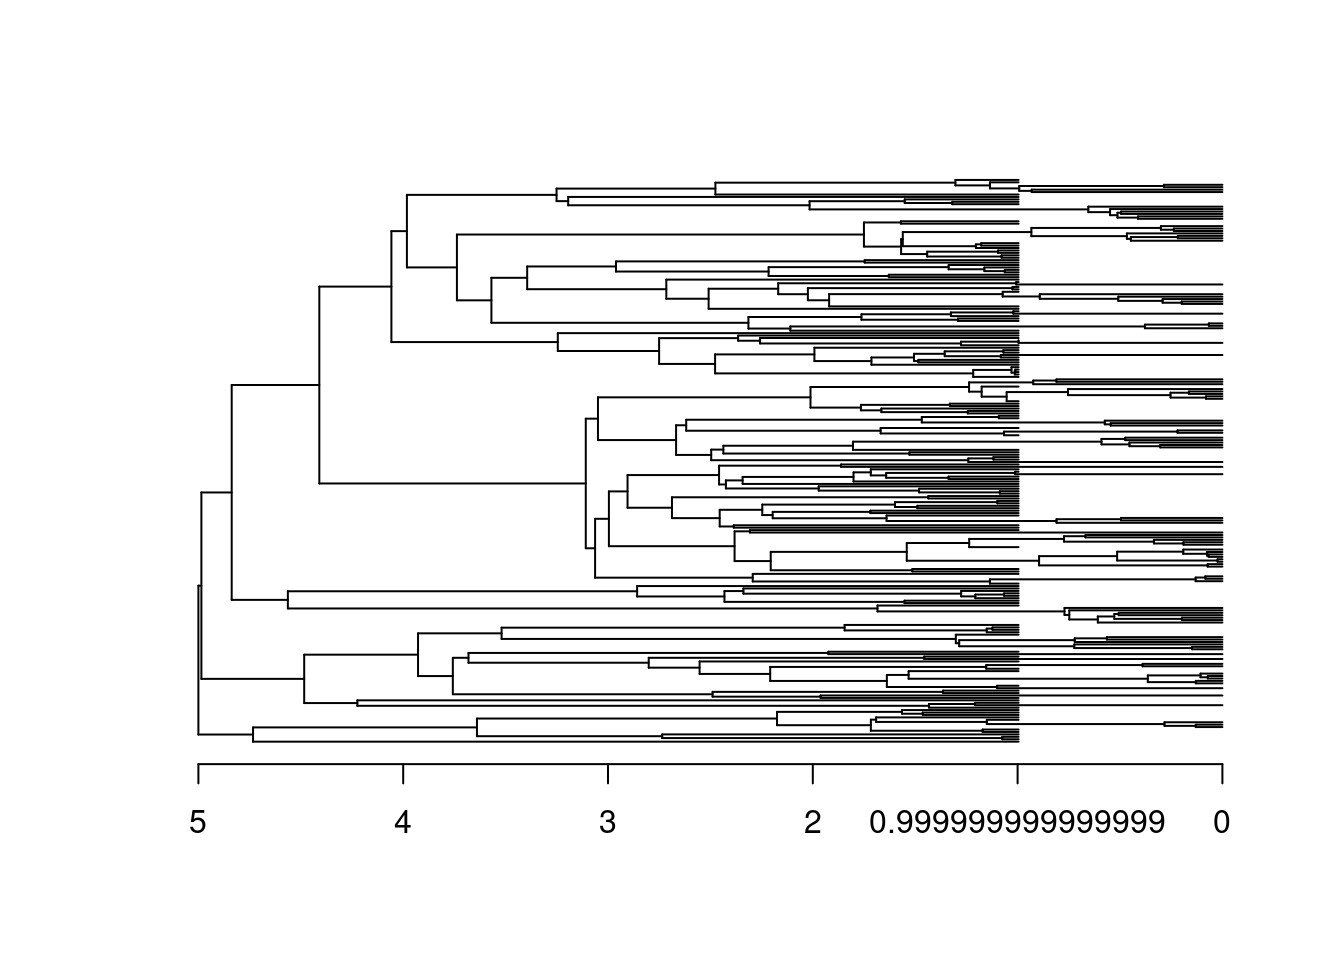
\includegraphics{treats_manual_files/figure-latex/unnamed-chunk-90-1.pdf}

Or for a slightly more complex example, we can can change the trait process from a BM to an OU when the trait values reaches an upper 95\% quantile value above 2:

\begin{Shaded}
\begin{Highlighting}[]
\CommentTok{\#\# The 95\% upper quantile value of a distribution}
\NormalTok{upper}\FloatTok{.95}\NormalTok{ \textless{}{-}}\StringTok{ }\ControlFlowTok{function}\NormalTok{(x) \{}
    \KeywordTok{return}\NormalTok{(}\KeywordTok{quantile}\NormalTok{(x, }\DataTypeTok{prob =} \FloatTok{0.95}\NormalTok{))}
\NormalTok{\} }
\CommentTok{\#\# Create an event to change the trait process}
\NormalTok{change\_process \textless{}{-}}\StringTok{ }\KeywordTok{make.events}\NormalTok{(}
                  \DataTypeTok{target =} \StringTok{"traits"}\NormalTok{,}
                  \CommentTok{\#\# condition is triggered if(upper.95(x) \textgreater{} 3)}
                  \DataTypeTok{condition =} \KeywordTok{trait.condition}\NormalTok{(}\DecValTok{3}\NormalTok{, }\DataTypeTok{condition =} \StringTok{\textasciigrave{}}\DataTypeTok{\textgreater{}}\StringTok{\textasciigrave{}}\NormalTok{, }\DataTypeTok{what =}\NormalTok{ upper}\FloatTok{.95}\NormalTok{),}
                  \DataTypeTok{modification =} \KeywordTok{traits.update}\NormalTok{(}\DataTypeTok{process =}\NormalTok{ OU.process))}

\CommentTok{\#\# Set the simulation parameters}
\NormalTok{bd.params \textless{}{-}}\StringTok{ }\KeywordTok{list}\NormalTok{(}\DataTypeTok{extinction =} \DecValTok{0}\NormalTok{, }\DataTypeTok{speciation =} \DecValTok{1}\NormalTok{)}
\NormalTok{stop.rule \textless{}{-}}\StringTok{ }\KeywordTok{list}\NormalTok{(}\DataTypeTok{max.time =} \DecValTok{6}\NormalTok{)}
\NormalTok{traits    \textless{}{-}}\StringTok{ }\KeywordTok{make.traits}\NormalTok{()}

\CommentTok{\#\# Run the simulations}
\KeywordTok{set.seed}\NormalTok{(}\DecValTok{1}\NormalTok{)}
\NormalTok{no\_change \textless{}{-}}\StringTok{ }\KeywordTok{treats}\NormalTok{(}\DataTypeTok{bd.params =}\NormalTok{ bd.params,}
                  \DataTypeTok{stop.rule =}\NormalTok{ stop.rule,}
                  \DataTypeTok{traits =}\NormalTok{ traits)}
\KeywordTok{set.seed}\NormalTok{(}\DecValTok{1}\NormalTok{)}
\NormalTok{process\_change \textless{}{-}}\StringTok{ }\KeywordTok{treats}\NormalTok{(}\DataTypeTok{bd.params =}\NormalTok{ bd.params,}
                       \DataTypeTok{stop.rule =}\NormalTok{ stop.rule,}
                       \DataTypeTok{traits =}\NormalTok{ traits,}
                       \DataTypeTok{events =}\NormalTok{ change\_process)}
\CommentTok{\#\# Plot the results}
\KeywordTok{par}\NormalTok{(}\DataTypeTok{mfrow =} \KeywordTok{c}\NormalTok{(}\DecValTok{1}\NormalTok{,}\DecValTok{2}\NormalTok{))}
\KeywordTok{plot}\NormalTok{(no\_change, }\DataTypeTok{ylim =} \KeywordTok{c}\NormalTok{(}\OperatorTok{{-}}\DecValTok{7}\NormalTok{, }\DecValTok{7}\NormalTok{))}
\KeywordTok{plot}\NormalTok{(process\_change, }\DataTypeTok{ylim =} \KeywordTok{c}\NormalTok{(}\OperatorTok{{-}}\DecValTok{7}\NormalTok{, }\DecValTok{7}\NormalTok{))}
\end{Highlighting}
\end{Shaded}

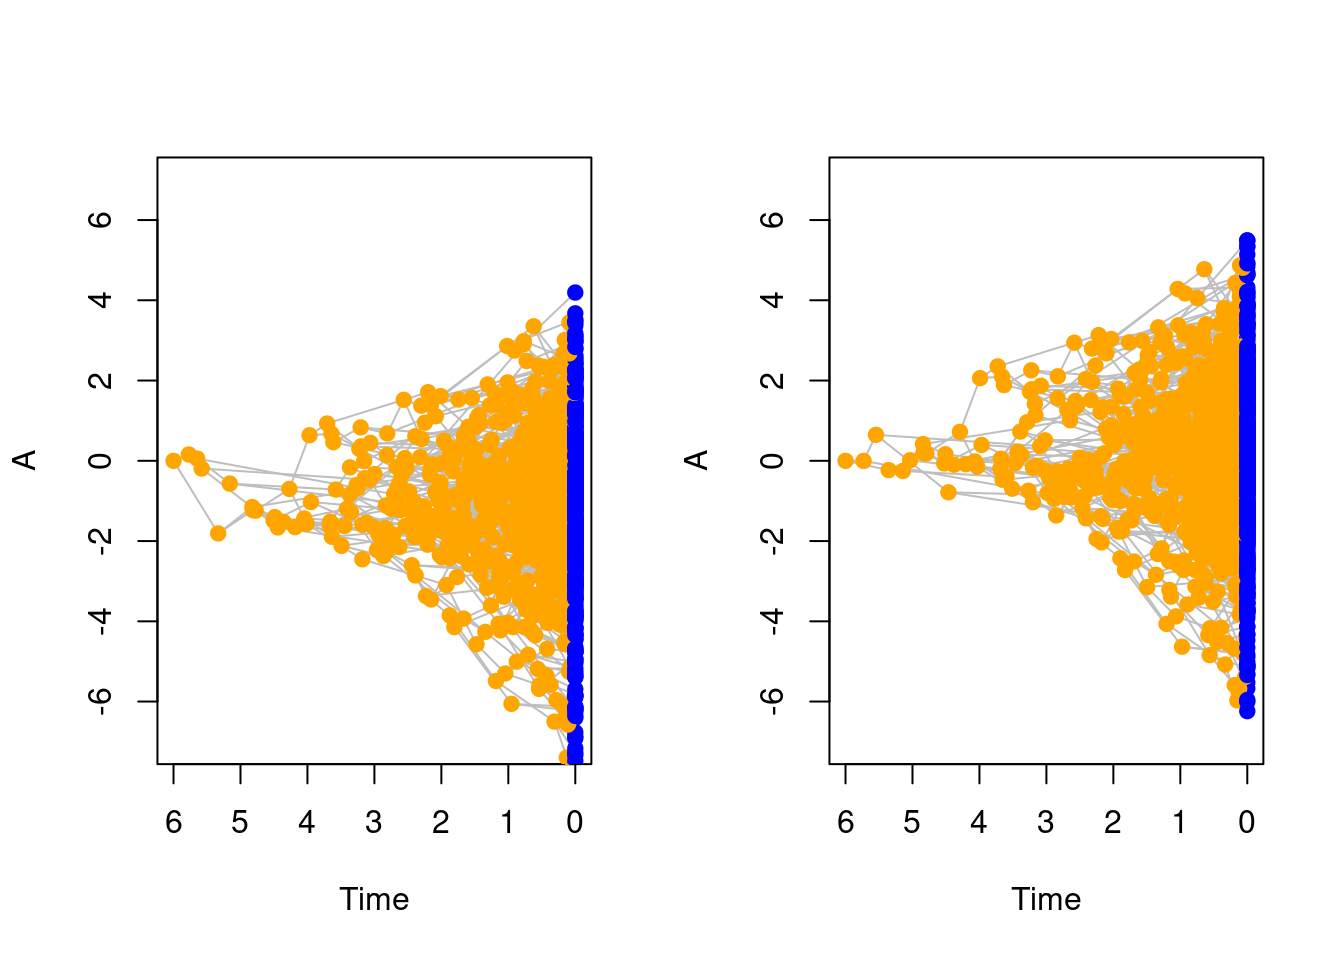
\includegraphics{treats_manual_files/figure-latex/unnamed-chunk-91-1.pdf}

\begin{Shaded}
\begin{Highlighting}[]
\KeywordTok{par}\NormalTok{(}\DataTypeTok{mfrow =} \KeywordTok{c}\NormalTok{(}\DecValTok{1}\NormalTok{,}\DecValTok{1}\NormalTok{))}
\end{Highlighting}
\end{Shaded}

\hypertarget{founding}{%
\section{Founding events}\label{founding}}

Founding events are a specific \texttt{target} for \texttt{events} that allows you to simulate a birth-death process within the current one!
It allows you to simulate a specific \texttt{treats} process using the \texttt{treats} function with its own \texttt{traits}, \texttt{modifiers}, \texttt{bd.params} and \texttt{events} (and yes, that's including \texttt{events} that have their own \texttt{founding} event).
This is basically the ultimate nested boss of modularity!

The founding event will run an internal \texttt{treats} process (i.e.~simulating a tree and, optionally, some data) resulting in a founding sub-tree.
It will then branch this sub-tree onto the rest of the simulation that continued normally in the mean time.
You can specify the founding event using the inbuilt \texttt{founding.event} modification event.
This function takes the exact same arguments as \texttt{treats} to simulate the sub-tree with its own parameters.
Additionally, we will use the \texttt{additional.args} argument from \texttt{make.events} to specify a prefix for the founding tree tips (to make them easier to distinguish).

\begin{Shaded}
\begin{Highlighting}[]
\CommentTok{\#\# Set up parameters}
\NormalTok{stop.rule \textless{}{-}}\StringTok{ }\KeywordTok{list}\NormalTok{(}\DataTypeTok{max.time =} \DecValTok{4}\NormalTok{)}
\NormalTok{bd.params \textless{}{-}}\StringTok{ }\KeywordTok{make.bd.params}\NormalTok{(}\DataTypeTok{speciation =} \DecValTok{1}\NormalTok{, }\DataTypeTok{extinction =} \FloatTok{0.3}\NormalTok{)}

\CommentTok{\#\# Events that generate a new process (founding tree {-} with no extinction)}
\NormalTok{founding\_event \textless{}{-}}\StringTok{ }\KeywordTok{make.events}\NormalTok{(}
                  \DataTypeTok{target =} \StringTok{"founding"}\NormalTok{,}
                  \DataTypeTok{condition =} \KeywordTok{taxa.condition}\NormalTok{(}\DecValTok{10}\NormalTok{),}
                  \DataTypeTok{modification =} \KeywordTok{founding.event}\NormalTok{(}
                                    \DataTypeTok{bd.params =} \KeywordTok{make.bd.params}\NormalTok{(}\DataTypeTok{speciation =} \DecValTok{2}\NormalTok{,}
                                                               \DataTypeTok{extinction =} \DecValTok{0}\NormalTok{)),}
                  \DataTypeTok{additional.args =} \KeywordTok{list}\NormalTok{(}\DataTypeTok{prefix =} \StringTok{"founding\_"}\NormalTok{))}
    
\CommentTok{\#\# Simulations}
\KeywordTok{set.seed}\NormalTok{(}\DecValTok{11}\NormalTok{)}
\NormalTok{founding\_tree \textless{}{-}}\StringTok{ }\KeywordTok{treats}\NormalTok{(}\DataTypeTok{bd.params =}\NormalTok{ bd.params,}
                      \DataTypeTok{stop.rule =}\NormalTok{ stop.rule,}
                      \DataTypeTok{events =}\NormalTok{ founding\_event)}
\KeywordTok{plot}\NormalTok{(founding\_tree, }\DataTypeTok{cex =} \FloatTok{0.4}\NormalTok{)}
\end{Highlighting}
\end{Shaded}

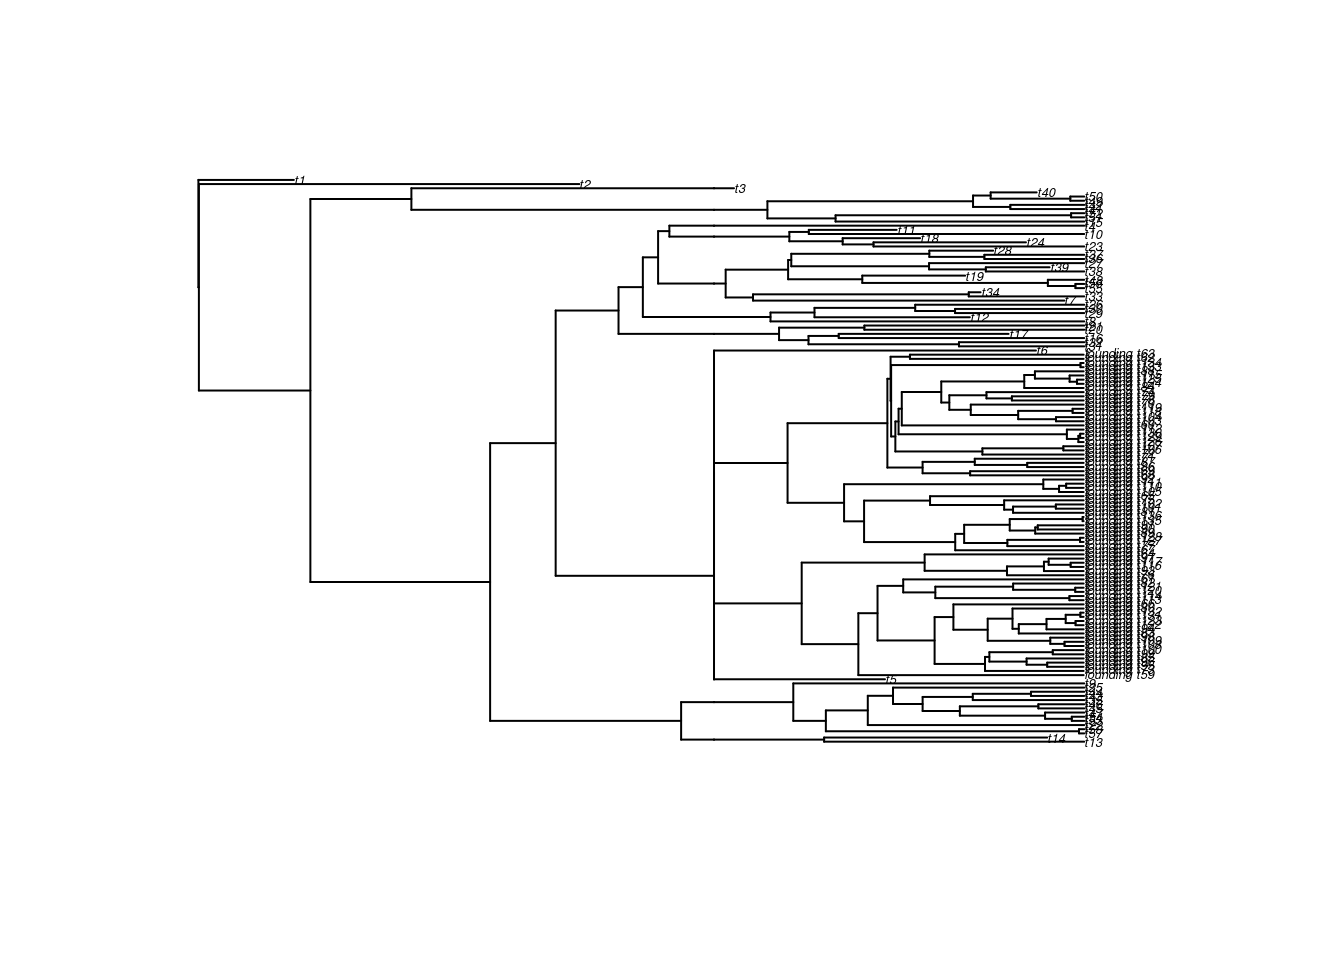
\includegraphics{treats_manual_files/figure-latex/unnamed-chunk-92-1.pdf}

Note that the nestedness here is potentially endless, for example, you can pass an \texttt{event} argument to the \texttt{founding.event} that will generate another founding event, etc.

\hypertarget{others}{%
\chapter{Other functionalities}\label{others}}

\hypertarget{makebdparams}{%
\section{\texorpdfstring{\texttt{make.bd.params}}{make.bd.params}}\label{makebdparams}}

In most examples above, birth-death parameters were set as fixed values, i.e.~a speciation rate of \(\lambda\) and an extinction rate of \(\mu\) throughout the simulations (with maybe some events modifying these rates).
However, it is possible to set these rates as specific or changing distributions.
You can do this using the \texttt{make.bd.params} function to provide either a \texttt{vector} of values:

\begin{Shaded}
\begin{Highlighting}[]
\CommentTok{\#\# An example where the speciation is randomly sampled among three values}
\NormalTok{my\_bd\_params \textless{}{-}}\StringTok{ }\KeywordTok{make.bd.params}\NormalTok{(}\DataTypeTok{speciation =} \KeywordTok{c}\NormalTok{(}\DecValTok{1}\OperatorTok{/}\DecValTok{3}\NormalTok{,}\DecValTok{42}\NormalTok{))}

\CommentTok{\#\# Building a tree using this set of parameters}
\KeywordTok{set.seed}\NormalTok{(}\DecValTok{123}\NormalTok{)}
\KeywordTok{plot}\NormalTok{(}\KeywordTok{treats}\NormalTok{(}\DataTypeTok{stop.rule =} \KeywordTok{list}\NormalTok{(}\DataTypeTok{max.taxa =} \DecValTok{50}\NormalTok{), }\DataTypeTok{bd.params =}\NormalTok{ my\_bd\_params))}
\end{Highlighting}
\end{Shaded}

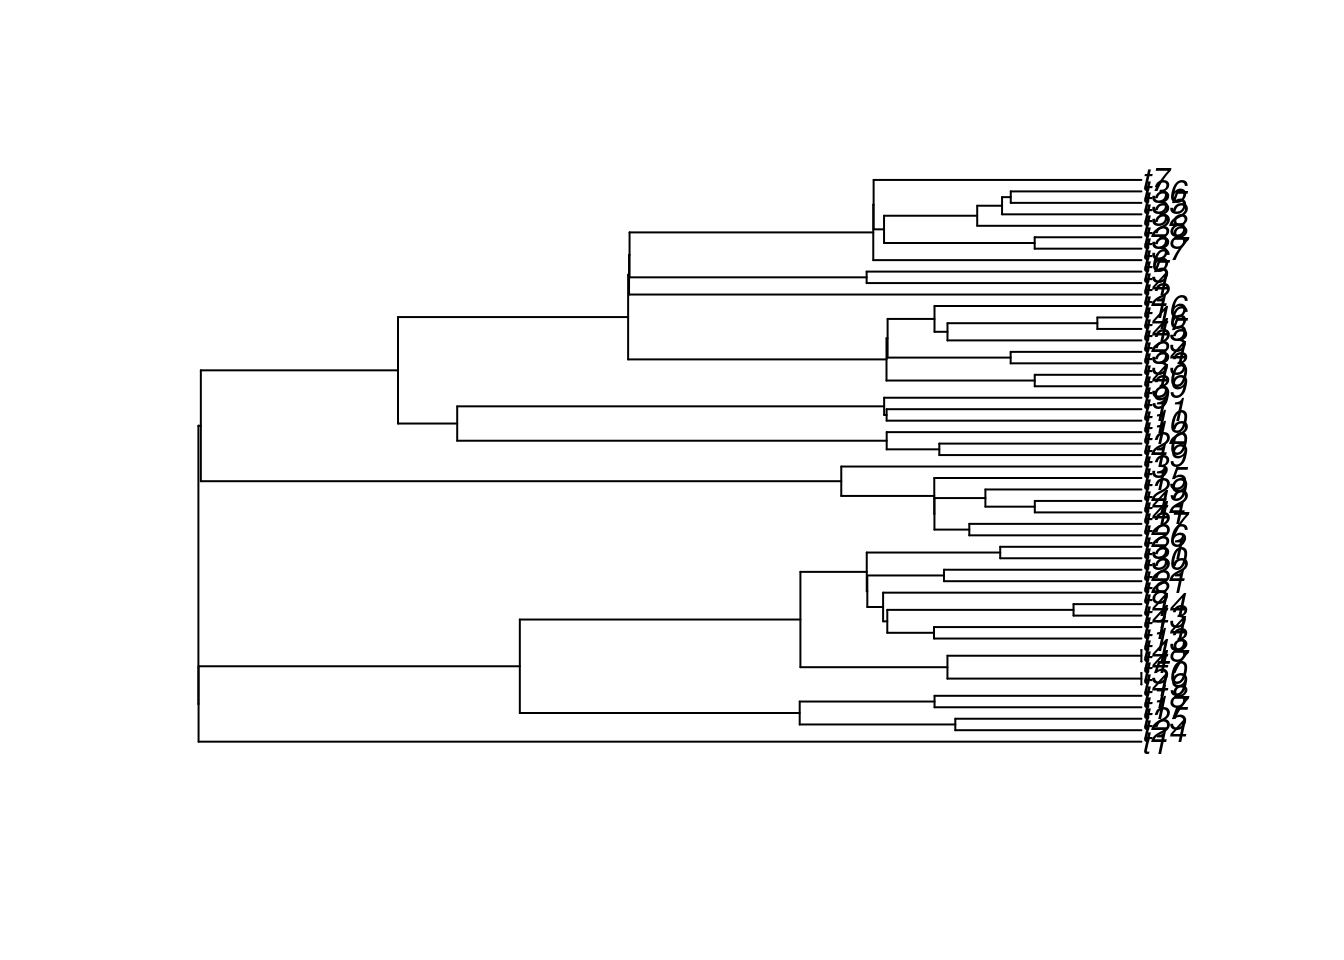
\includegraphics{treats_manual_files/figure-latex/unnamed-chunk-94-1.pdf}

\begin{Shaded}
\begin{Highlighting}[]
\CommentTok{\#\# Note the regions in the tree with short branches}
\CommentTok{\#\# (that\textquotesingle{}s the speciation being 1/3 while the others are speciation = 42) }
\end{Highlighting}
\end{Shaded}

Or to directly provide a function from which to sample:

\begin{Shaded}
\begin{Highlighting}[]
\CommentTok{\#\# Another example where speciation is drawn from the interval (0, 1)}
\KeywordTok{make.bd.params}\NormalTok{(}\DataTypeTok{speciation =}\NormalTok{ runif)}
\end{Highlighting}
\end{Shaded}

\begin{verbatim}
##  ---- treats birth-death parameters object ---- 
## speciation: runif.
## extinction: 0.
\end{verbatim}

In this example, the \texttt{"bd.params"} object passed to the \texttt{treats} function will allow the birth-death process to sample the speciation parameter each time it is called (e.g.~during the speciation/extinction step, the branch length step, etc.).
If using a function, you can fine tune the arguments to be passed to that function using the \texttt{speciation.args} or the \texttt{extinction.args} arguments (as a named list matching the function's arguments):

\begin{Shaded}
\begin{Highlighting}[]
\CommentTok{\#\# Speciation is drawn from the interval (0.5, 1.5)}
\KeywordTok{make.bd.params}\NormalTok{(}\DataTypeTok{speciation =}\NormalTok{ runif,}
               \DataTypeTok{speciation.args =} \KeywordTok{list}\NormalTok{(}\DataTypeTok{min =} \FloatTok{0.5}\NormalTok{, }\DataTypeTok{max =} \FloatTok{1.5}\NormalTok{))}
\end{Highlighting}
\end{Shaded}

\begin{verbatim}
##  ---- treats birth-death parameters object ---- 
## speciation: runif (with optional arguments).
## extinction: 0.
\end{verbatim}

When using distributions for both the speciation and extinction parameters, you can run into the (usually) undesired problem of having an extinction rate that is higher than your speciation rate and thus all the taxa in your tree dying out.
You can avoid this problem by using the \texttt{joint} distribution argument.
This will ensure that the sampling of the extinction rate is always lower or equal to the speciation rate.

\begin{Shaded}
\begin{Highlighting}[]
\CommentTok{\#\# Joint speciation and extinction sampled from uniform distribution }
\CommentTok{\#\# with speciation always \textgreater{}= to extinction}
\KeywordTok{make.bd.params}\NormalTok{(}\DataTypeTok{speciation =}\NormalTok{ runif, }\DataTypeTok{extinction =}\NormalTok{ runif, }\DataTypeTok{joint =} \OtherTok{TRUE}\NormalTok{)}
\end{Highlighting}
\end{Shaded}

\begin{verbatim}
##  ---- treats birth-death parameters object ---- 
## joint sampling for:
## speciation: runif.
## extinction: runif.
\end{verbatim}

Finally to avoid negative sampling values, you can use the argument \texttt{absolute} that will make all the sampled values positive.
This argument is set to \texttt{TRUE} by default so you shouldn't have to worry about it most of the time unless you specifically need negative sampled values for your parameters.

\begin{Shaded}
\begin{Highlighting}[]
\CommentTok{\#\# Making the speciation sampling always positive}
\KeywordTok{make.bd.params}\NormalTok{(}\DataTypeTok{speciation =}\NormalTok{ rnorm, }\DataTypeTok{absolute =} \OtherTok{TRUE}\NormalTok{)}
\end{Highlighting}
\end{Shaded}

\begin{verbatim}
##  ---- treats birth-death parameters object ---- 
## speciation: rnorm.
## extinction: 0.
## (using absolute values)
\end{verbatim}

The two other possible arguments for this function are \texttt{test} and \texttt{update} that work the same way as \protect\hyperlink{maketraits}{\texttt{make.traits}} or \protect\hyperlink{makemodifiers}{\texttt{make.modifiers}}

If you are a visual person and your \texttt{bd.params} objects are getting a bit too complicated to remember, you can always quickly plot them.
The function will sample from the \texttt{bd.params} object and show the results:

\begin{Shaded}
\begin{Highlighting}[]
\KeywordTok{par}\NormalTok{(}\DataTypeTok{mfrow =} \KeywordTok{c}\NormalTok{(}\DecValTok{2}\NormalTok{,}\DecValTok{3}\NormalTok{))}
\KeywordTok{plot}\NormalTok{(}\KeywordTok{make.bd.params}\NormalTok{(), }\DataTypeTok{main =} \StringTok{"Default birth{-}death parameters"}\NormalTok{)}
\KeywordTok{plot}\NormalTok{(}\KeywordTok{make.bd.params}\NormalTok{(}\DataTypeTok{speciation =}\NormalTok{ runif,}
               \DataTypeTok{speciation.args =} \KeywordTok{list}\NormalTok{(}\DataTypeTok{min =} \FloatTok{0.5}\NormalTok{, }\DataTypeTok{max =} \FloatTok{1.5}\NormalTok{)),}
     \DataTypeTok{main =} \StringTok{"Uniform speciation between 0.5 and 1.5}\CharTok{\textbackslash{}n}\StringTok{(no extinction)"}\NormalTok{)}
\KeywordTok{plot}\NormalTok{(}\KeywordTok{make.bd.params}\NormalTok{(}\DataTypeTok{speciation =}\NormalTok{ runif,}
                    \DataTypeTok{speciation.args =} \KeywordTok{list}\NormalTok{(}\DataTypeTok{min =} \FloatTok{0.5}\NormalTok{, }\DataTypeTok{max =} \FloatTok{1.5}\NormalTok{)),}
     \DataTypeTok{main =} \StringTok{"Uniform speciation between 0.5 and 1.5}\CharTok{\textbackslash{}n}\StringTok{(no extinction)"}\NormalTok{)}
\KeywordTok{plot}\NormalTok{(}\KeywordTok{make.bd.params}\NormalTok{(}\DataTypeTok{speciation =}\NormalTok{ runif, }\DataTypeTok{extinction =}\NormalTok{ runif, }\DataTypeTok{joint =} \OtherTok{TRUE}\NormalTok{),}
     \DataTypeTok{main =} \StringTok{"Joint uniform speciation and extinction"}\NormalTok{)}
\KeywordTok{plot}\NormalTok{(}\KeywordTok{make.bd.params}\NormalTok{(}\DataTypeTok{speciation =}\NormalTok{ rnorm, }\DataTypeTok{extinction =}\NormalTok{ runif,}
                    \DataTypeTok{joint =} \OtherTok{FALSE}\NormalTok{, }\DataTypeTok{abs =} \OtherTok{FALSE}\NormalTok{),}
     \DataTypeTok{main =} \StringTok{"Disjoint normal speciation and uniform extinction"}\NormalTok{)}
\KeywordTok{par}\NormalTok{(}\DataTypeTok{mfrow =} \KeywordTok{c}\NormalTok{(}\DecValTok{1}\NormalTok{,}\DecValTok{1}\NormalTok{))}
\end{Highlighting}
\end{Shaded}

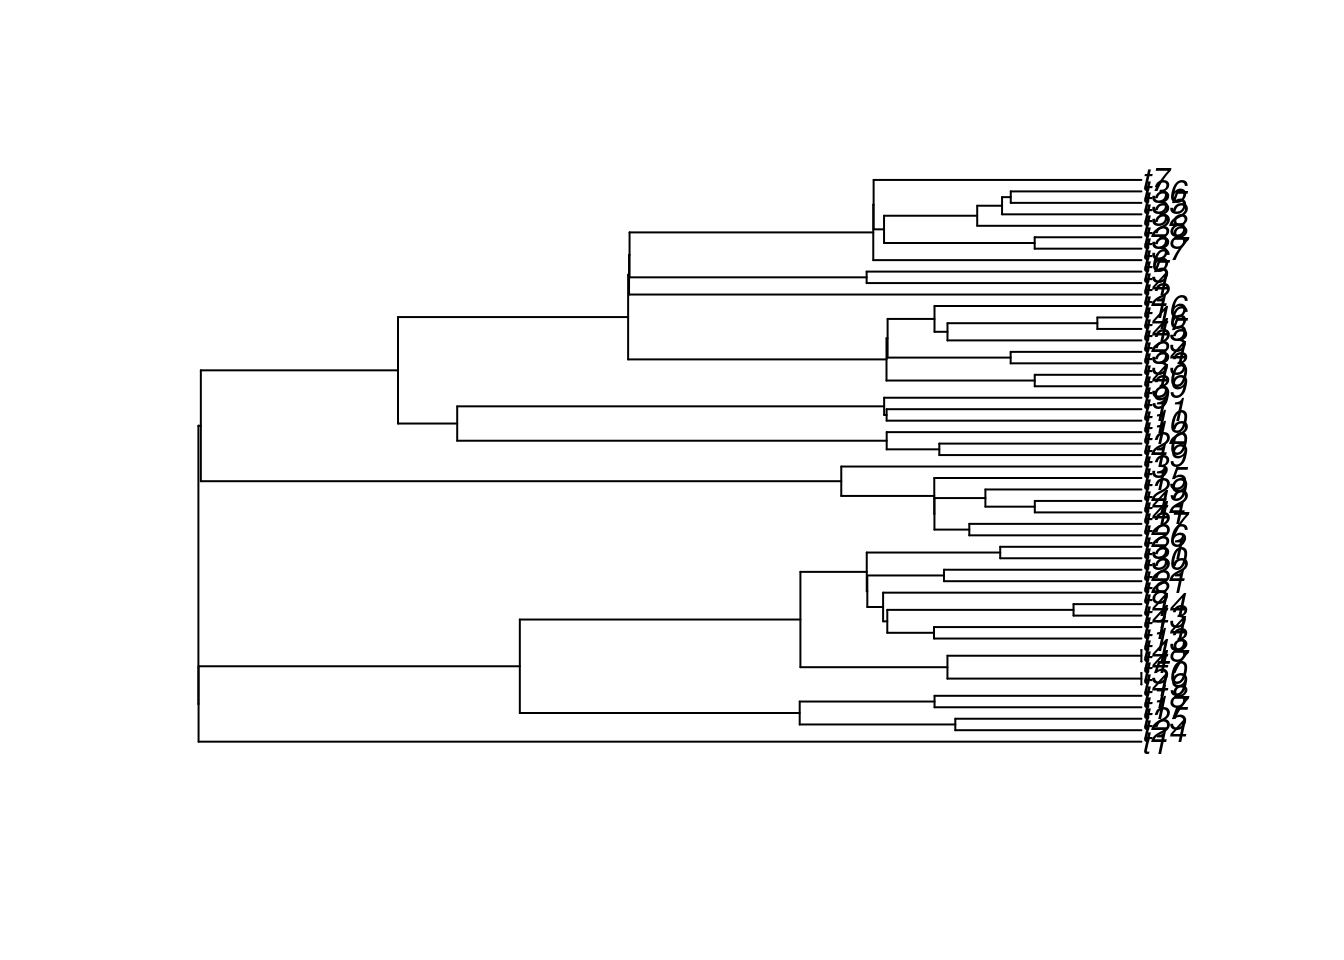
\includegraphics{treats_manual_files/figure-latex/unnamed-chunk-99-1.pdf}

\hypertarget{dropthings}{%
\section{\texorpdfstring{\texttt{drop.things}}{drop.things}}\label{dropthings}}

You can use the function \texttt{drop.things} to drop specific elements of the tree and data at the same time by providing the argument \texttt{what\ =\ "fossils"} for tips that went extinct, or \texttt{what\ =\ "livings"} for tips that where alive at the end of the simulation or \texttt{what\ =\ "singles"} to drop internal singleton nodes.
Alternatively you can use the function aliases \texttt{drop.fossils}, \texttt{drop.livings} or \texttt{drop.singles} for the exact same results:

\begin{Shaded}
\begin{Highlighting}[]
\CommentTok{\#\# A random tree with fossils and traits and internal nodes every 0.5 times}
\KeywordTok{set.seed}\NormalTok{(}\DecValTok{3}\NormalTok{)}
\NormalTok{my\_data \textless{}{-}}\StringTok{ }\KeywordTok{treats}\NormalTok{(}\DataTypeTok{stop.rule =} \KeywordTok{list}\NormalTok{(}\DataTypeTok{max.taxa =} \DecValTok{20}\NormalTok{),}
                \DataTypeTok{bd.params =} \KeywordTok{list}\NormalTok{(}\DataTypeTok{speciation =} \DecValTok{1}\NormalTok{, }\DataTypeTok{extinction =} \DecValTok{1}\OperatorTok{/}\DecValTok{3}\NormalTok{),}
                \DataTypeTok{traits    =} \KeywordTok{make.traits}\NormalTok{(), }\DataTypeTok{save.steps =} \FloatTok{0.5}\NormalTok{)}

\CommentTok{\#\# A tree with 20 tips and 54 nodes}
\NormalTok{my\_data}\OperatorTok{$}\NormalTok{tree}
\end{Highlighting}
\end{Shaded}

\begin{verbatim}
## 
## Phylogenetic tree with 20 tips and 54 internal nodes.
## 
## Tip labels:
##   t1, t2, t3, t4, t5, t6, ...
## Node labels:
##   n1, n2, n3, n4, n5, n6, ...
## 
## Rooted; includes branch lengths.
\end{verbatim}

\begin{Shaded}
\begin{Highlighting}[]
\CommentTok{\#\# And a dataset with 74 rows}
\KeywordTok{dim}\NormalTok{(my\_data}\OperatorTok{$}\NormalTok{data)}
\end{Highlighting}
\end{Shaded}

\begin{verbatim}
## [1] 74  1
\end{verbatim}

\begin{Shaded}
\begin{Highlighting}[]
\CommentTok{\#\# Removing the fossil species}
\KeywordTok{drop.things}\NormalTok{(my\_data, }\DataTypeTok{what =} \StringTok{"fossils"}\NormalTok{)}\OperatorTok{$}\NormalTok{tree}
\end{Highlighting}
\end{Shaded}

\begin{verbatim}
## 
## Phylogenetic tree with 8 tips and 31 internal nodes.
## 
## Tip labels:
##   t13, t14, t15, t16, t17, t18, ...
## Node labels:
##   n1, n2, n7, n10, n11, n13, ...
## 
## Rooted; includes branch lengths.
\end{verbatim}

\begin{Shaded}
\begin{Highlighting}[]
\KeywordTok{dim}\NormalTok{(}\KeywordTok{drop.fossils}\NormalTok{(my\_data)}\OperatorTok{$}\NormalTok{data)}
\end{Highlighting}
\end{Shaded}

\begin{verbatim}
## [1] 39  1
\end{verbatim}

\begin{Shaded}
\begin{Highlighting}[]
\CommentTok{\#\# Removing the living species}
\KeywordTok{drop.things}\NormalTok{(my\_data, }\DataTypeTok{what =} \StringTok{"livings"}\NormalTok{)}\OperatorTok{$}\NormalTok{tree}
\end{Highlighting}
\end{Shaded}

\begin{verbatim}
## 
## Phylogenetic tree with 12 tips and 37 internal nodes.
## 
## Tip labels:
##   t1, t2, t3, t4, t5, t6, ...
## Node labels:
##   n1, n2, n3, n4, n5, n6, ...
## 
## Rooted; includes branch lengths.
\end{verbatim}

\begin{Shaded}
\begin{Highlighting}[]
\KeywordTok{dim}\NormalTok{(}\KeywordTok{drop.livings}\NormalTok{(my\_data)}\OperatorTok{$}\NormalTok{data)}
\end{Highlighting}
\end{Shaded}

\begin{verbatim}
## [1] 49  1
\end{verbatim}

\begin{Shaded}
\begin{Highlighting}[]
\CommentTok{\#\# Removing the internal nodes}
\KeywordTok{drop.things}\NormalTok{(my\_data, }\DataTypeTok{what =} \StringTok{"singles"}\NormalTok{)}\OperatorTok{$}\NormalTok{tree}
\end{Highlighting}
\end{Shaded}

\begin{verbatim}
## 
## Phylogenetic tree with 20 tips and 19 internal nodes.
## 
## Tip labels:
##   t1, t2, t3, t4, t5, t6, ...
## Node labels:
##   n1, n7, n33, n39, n54, n40, ...
## 
## Rooted; includes branch lengths.
\end{verbatim}

\begin{Shaded}
\begin{Highlighting}[]
\KeywordTok{dim}\NormalTok{(}\KeywordTok{drop.singles}\NormalTok{(my\_data)}\OperatorTok{$}\NormalTok{data)}
\end{Highlighting}
\end{Shaded}

\begin{verbatim}
## [1] 39  1
\end{verbatim}

\begin{Shaded}
\begin{Highlighting}[]
\CommentTok{\#\# Removing the internal nodes AND the fossils}
\KeywordTok{drop.singles}\NormalTok{(}\KeywordTok{drop.fossils}\NormalTok{(my\_data))}
\end{Highlighting}
\end{Shaded}

\begin{verbatim}
##  ---- treats object ---- 
## Simulated phylogenetic tree (x$tree):
## 
## Phylogenetic tree with 8 tips and 7 internal nodes.
## 
## Tip labels:
##   t13, t14, t15, t16, t17, t18, ...
## Node labels:
##   n7, n33, n54, n53, n34, n45, ...
## 
## Rooted; includes branch lengths.
## 
## Simulated trait data (x$data):
## 1 trait for 1 process (A) with one starting value (0).
\end{verbatim}

\hypertarget{treats-internal-utilities}{%
\section{\texorpdfstring{\texttt{"treats"} internal utilities}{"treats" internal utilities}}\label{treats-internal-utilities}}

The package also provides utilities for internal functions, namely for designing \texttt{modifiers} or \texttt{events} more easily.
These functions don't do anything useful on their own but are optimised to be used internally in \texttt{treats}.
For all these functions, you can look at the internal manual for an example (i.e.~using \texttt{?\textless{}function\_name\textgreater{}})

So far the package has the following internals:

\begin{longtable}[]{@{}lll@{}}
\toprule
\begin{minipage}[b]{0.20\columnwidth}\raggedright
Function\strut
\end{minipage} & \begin{minipage}[b]{0.28\columnwidth}\raggedright
What it does\strut
\end{minipage} & \begin{minipage}[b]{0.43\columnwidth}\raggedright
Where can it be used\strut
\end{minipage}\tabularnewline
\midrule
\endhead
\begin{minipage}[t]{0.20\columnwidth}\raggedright
\texttt{parent.traits}\strut
\end{minipage} & \begin{minipage}[t]{0.28\columnwidth}\raggedright
selects the trait values of the current lineage's parents (i.e.~direct ancestor)\strut
\end{minipage} & \begin{minipage}[t]{0.43\columnwidth}\raggedright
in \texttt{make.modifiers}\strut
\end{minipage}\tabularnewline
\begin{minipage}[t]{0.20\columnwidth}\raggedright
\texttt{taxa.condition}\strut
\end{minipage} & \begin{minipage}[t]{0.28\columnwidth}\raggedright
provides a trigger for an \texttt{event} dependent on the number of taxa\strut
\end{minipage} & \begin{minipage}[t]{0.43\columnwidth}\raggedright
in \texttt{make.events}\strut
\end{minipage}\tabularnewline
\begin{minipage}[t]{0.20\columnwidth}\raggedright
\texttt{age.condition}\strut
\end{minipage} & \begin{minipage}[t]{0.28\columnwidth}\raggedright
provides a trigger for an \texttt{event} dependent on time\strut
\end{minipage} & \begin{minipage}[t]{0.43\columnwidth}\raggedright
in \texttt{make.events}\strut
\end{minipage}\tabularnewline
\begin{minipage}[t]{0.20\columnwidth}\raggedright
\texttt{trait.condition}\strut
\end{minipage} & \begin{minipage}[t]{0.28\columnwidth}\raggedright
provides a trigger for an \texttt{event} dependent on trait values\strut
\end{minipage} & \begin{minipage}[t]{0.43\columnwidth}\raggedright
in \texttt{make.events}\strut
\end{minipage}\tabularnewline
\bottomrule
\end{longtable}

\hypertarget{plots}{%
\chapter{Plots}\label{plots}}

\texttt{"treats"} objects can be directly plotted in \texttt{treats} using the S3 \texttt{plot.treats} function (or just \texttt{plot(x)} if \texttt{x} is of class \texttt{"treats"}).

\hypertarget{plotting-traits}{%
\section{Plotting traits}\label{plotting-traits}}

\texttt{"treats"} \texttt{"traits"} objects are covered in the \protect\hyperlink{maketraits}{traits section}.
You can use \texttt{plot.treats} to plot them by choosing which specific trait to plot using the \texttt{trait} argument (default is 1):

\begin{Shaded}
\begin{Highlighting}[]
\CommentTok{\#\# Making a list of three traits}
\NormalTok{list\_of\_traits \textless{}{-}}\StringTok{ }\KeywordTok{make.traits}\NormalTok{(}\DataTypeTok{process =} \KeywordTok{c}\NormalTok{(no.process, BM.process, OU.process), }\DataTypeTok{trait.names =} \KeywordTok{c}\NormalTok{(}\StringTok{"No process (normal)"}\NormalTok{, }\StringTok{"Brownian motion"}\NormalTok{, }\StringTok{"Ornstein{-}Uhlenbeck"}\NormalTok{))}
\CommentTok{\#\# Plotting each trait separately}
\KeywordTok{par}\NormalTok{(}\DataTypeTok{mfrow =} \KeywordTok{c}\NormalTok{(}\DecValTok{2}\NormalTok{, }\DecValTok{2}\NormalTok{))}
\KeywordTok{plot}\NormalTok{(list\_of\_traits, }\DataTypeTok{trait =} \DecValTok{1}\NormalTok{)}
\CommentTok{\#\# Using different colours options}
\KeywordTok{plot}\NormalTok{(list\_of\_traits, }\DataTypeTok{trait =} \DecValTok{2}\NormalTok{, }\DataTypeTok{col =} \KeywordTok{c}\NormalTok{(}\StringTok{"red"}\NormalTok{, }\StringTok{"purple"}\NormalTok{, }\StringTok{"pink"}\NormalTok{))}
\CommentTok{\#\# Not using the default plot name}
\KeywordTok{plot}\NormalTok{(list\_of\_traits, }\DataTypeTok{trait =} \DecValTok{3}\NormalTok{, }\DataTypeTok{main =} \StringTok{"OU process"}\NormalTok{,}
     \DataTypeTok{cent.tend =}\NormalTok{ sd, }\DataTypeTok{quantiles =} \KeywordTok{c}\NormalTok{(}\DecValTok{10}\NormalTok{, }\DecValTok{30}\NormalTok{))}
\KeywordTok{par}\NormalTok{(}\DataTypeTok{mfrow =} \KeywordTok{c}\NormalTok{(}\DecValTok{1}\NormalTok{, }\DecValTok{1}\NormalTok{))}
\end{Highlighting}
\end{Shaded}

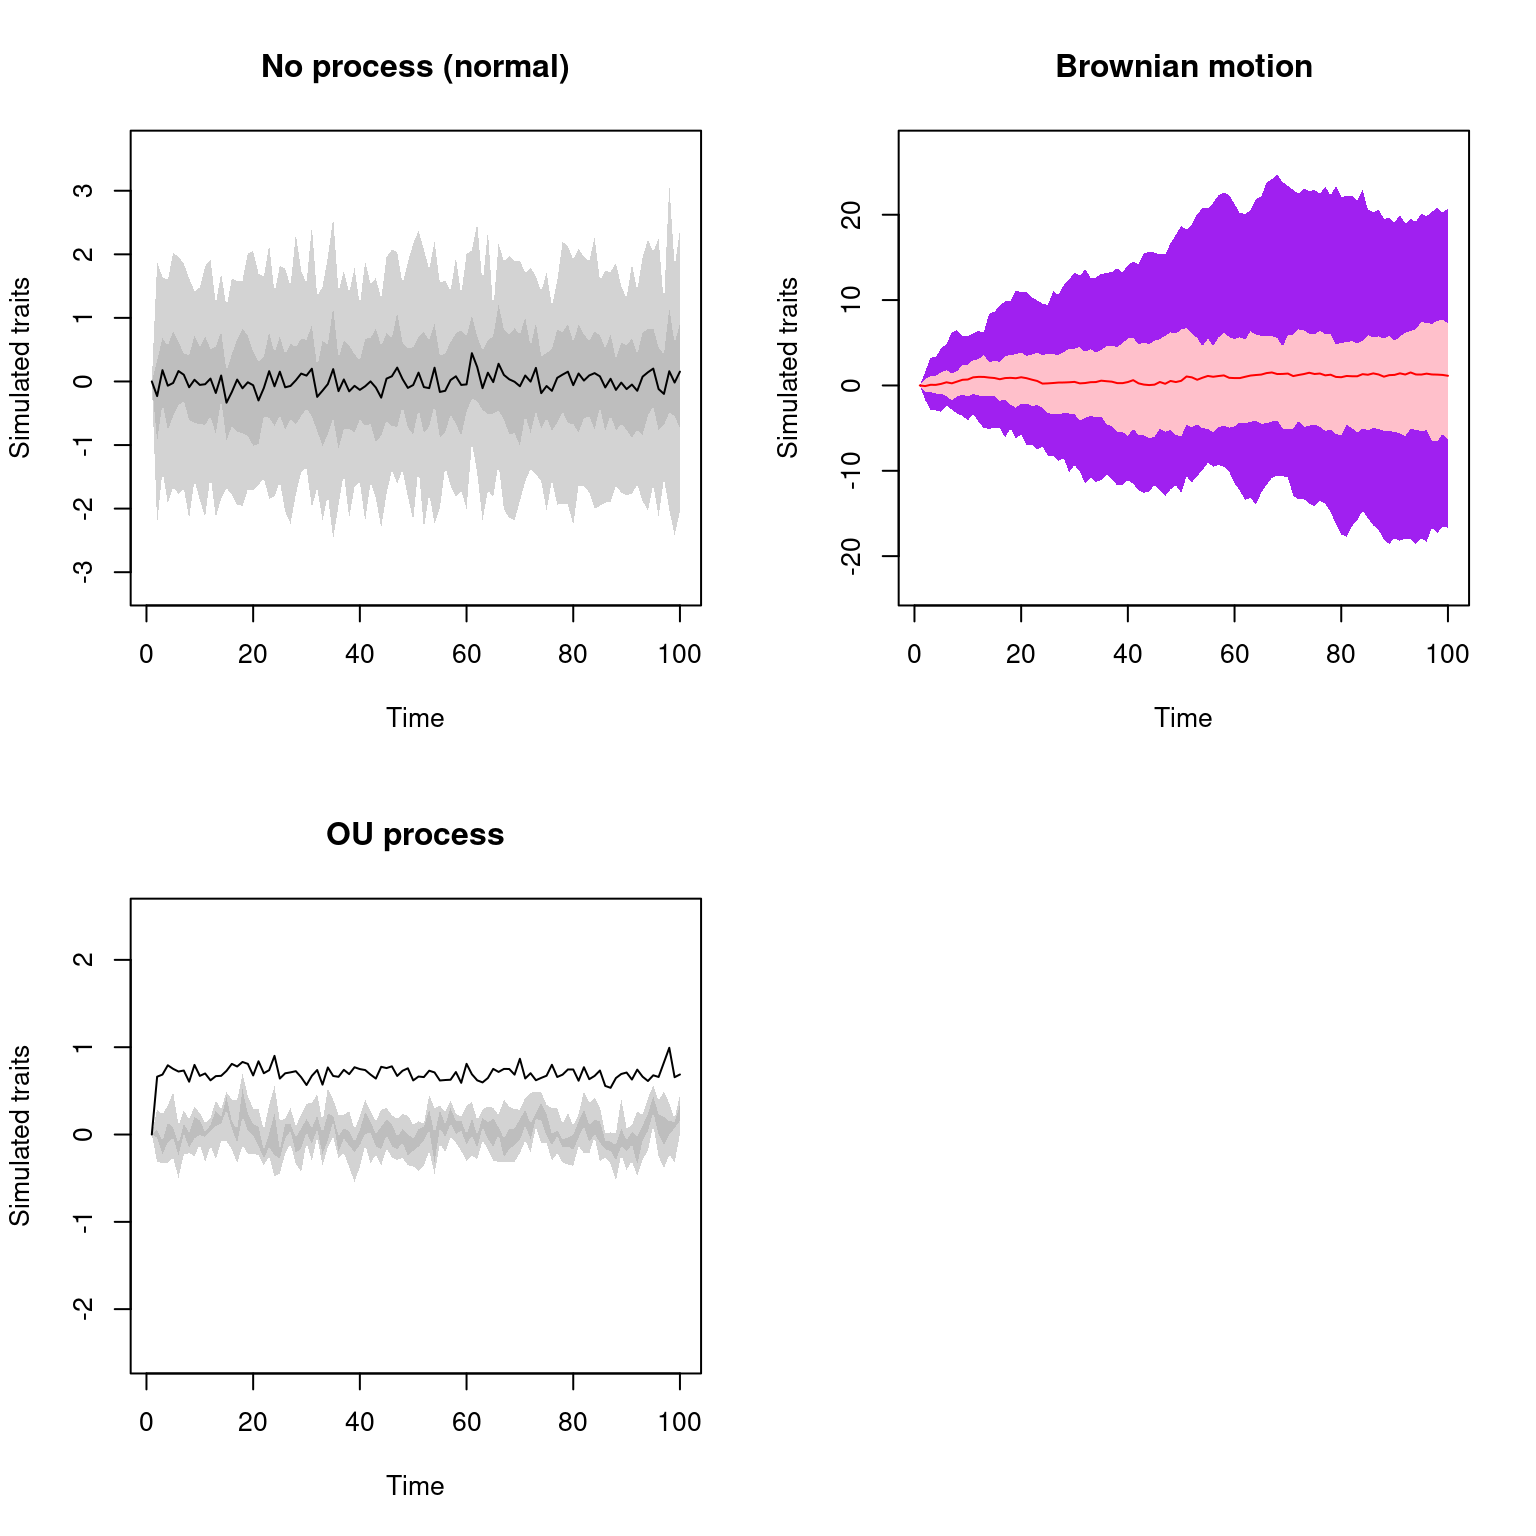
\includegraphics{treats_manual_files/figure-latex/unnamed-chunk-102-1.pdf}

You can also control the number of replicates in the simulation by using the \texttt{simulations} option (the default is 50).
Bigger numbers lead to more time but smoother looking plots while smaller ones are more stochastic:

\begin{Shaded}
\begin{Highlighting}[]
\KeywordTok{par}\NormalTok{(}\DataTypeTok{mfrow =} \KeywordTok{c}\NormalTok{(}\DecValTok{2}\NormalTok{,}\DecValTok{1}\NormalTok{))}
\KeywordTok{plot}\NormalTok{(list\_of\_traits, }\DataTypeTok{trait =} \DecValTok{2}\NormalTok{, }\DataTypeTok{simulations =} \DecValTok{10}\NormalTok{, }\DataTypeTok{main =} \StringTok{"10 BM simulations"}\NormalTok{)}
\KeywordTok{plot}\NormalTok{(list\_of\_traits, }\DataTypeTok{trait =} \DecValTok{2}\NormalTok{, }\DataTypeTok{simulations =} \DecValTok{1000}\NormalTok{, }\DataTypeTok{main =} \StringTok{"1k BM simulations"}\NormalTok{)}
\end{Highlighting}
\end{Shaded}

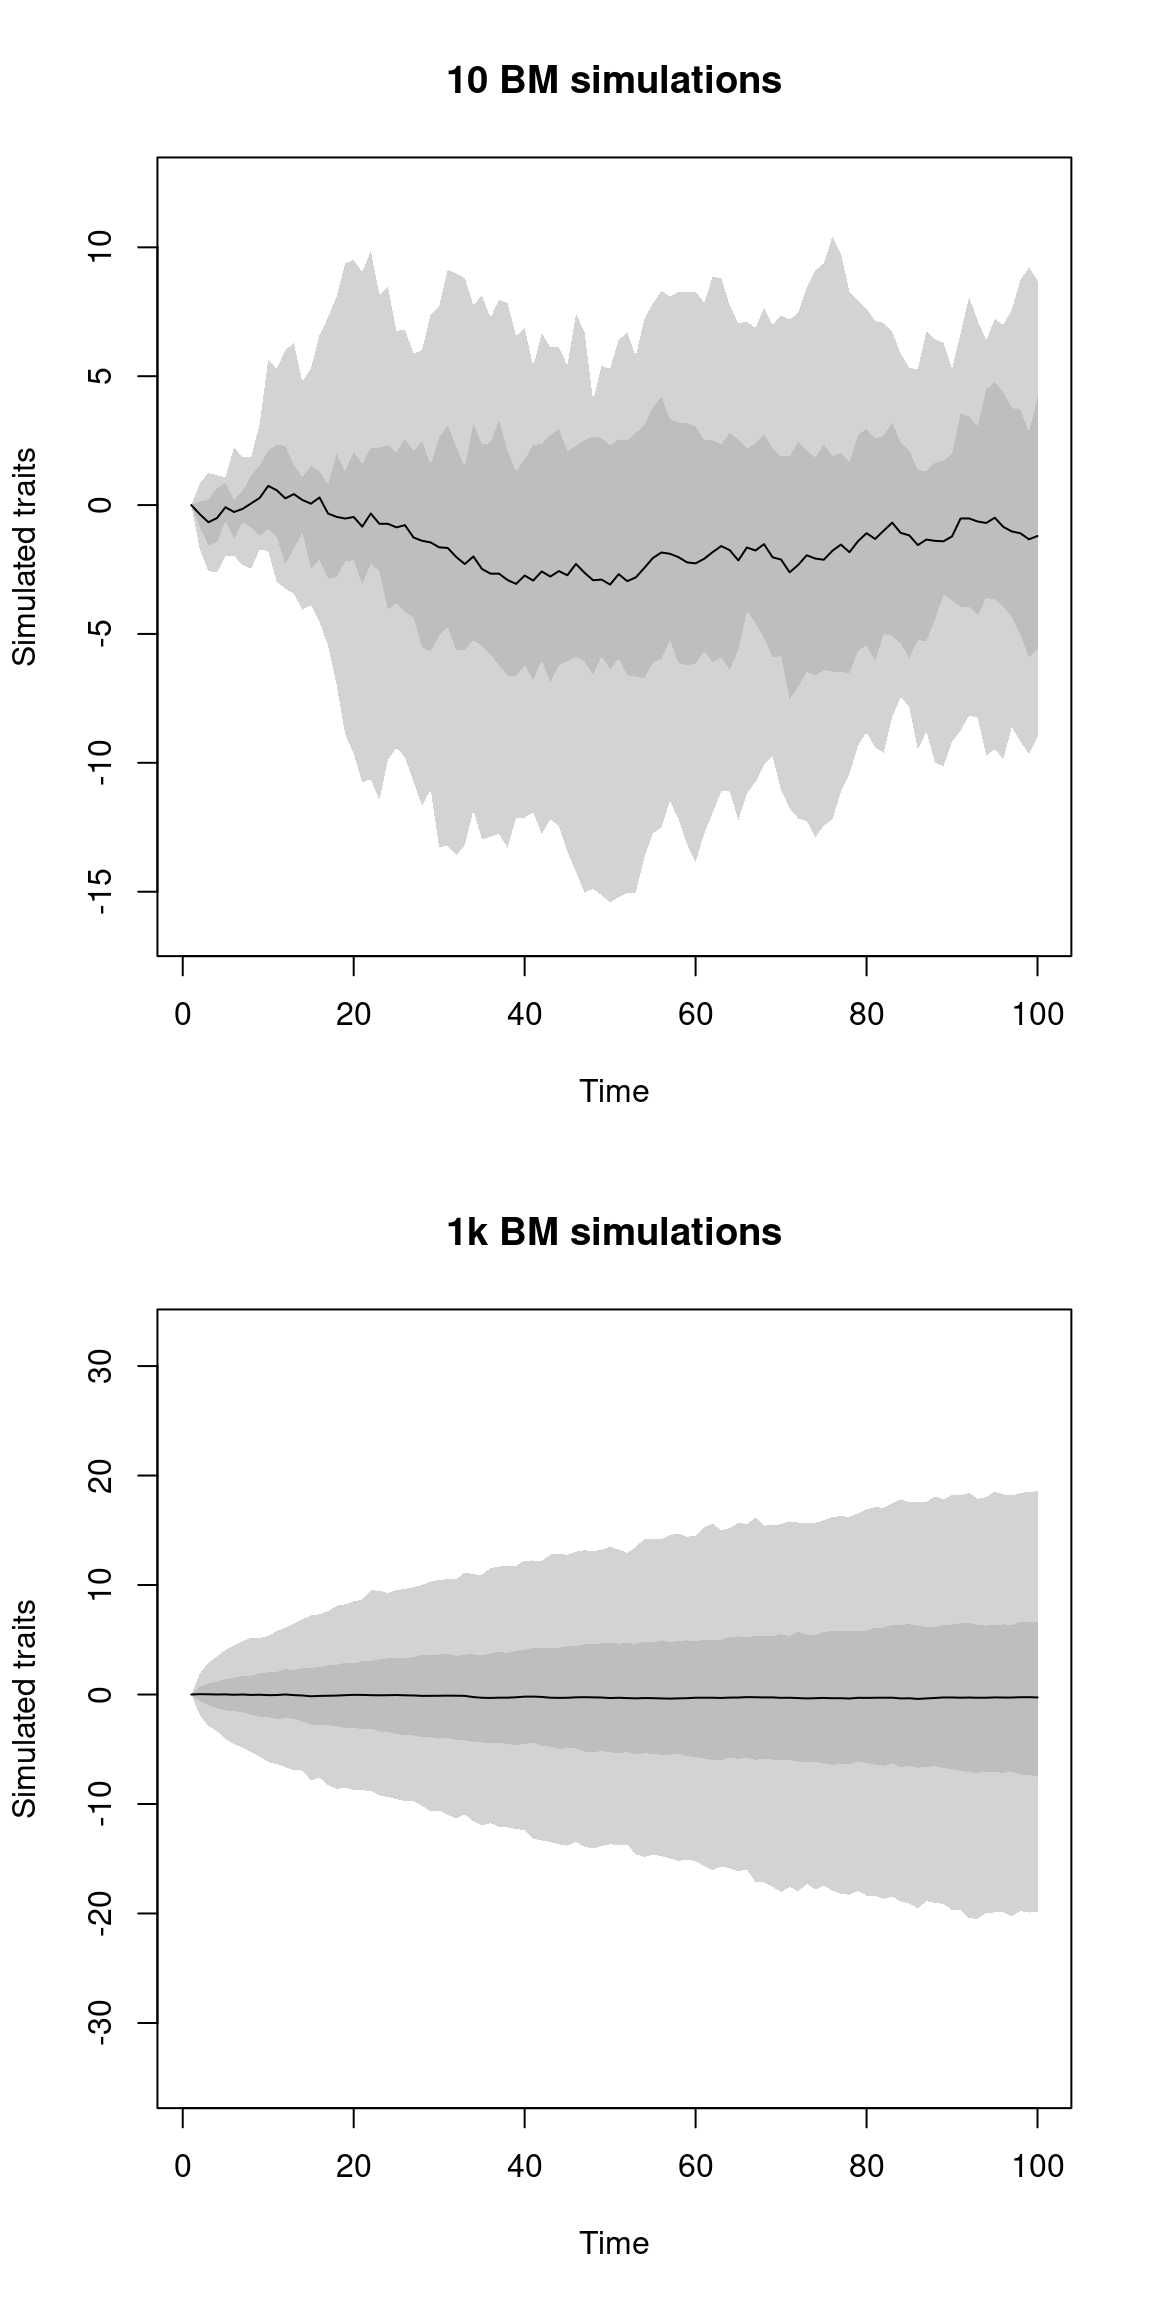
\includegraphics{treats_manual_files/figure-latex/unnamed-chunk-103-1.pdf}

\begin{Shaded}
\begin{Highlighting}[]
\KeywordTok{par}\NormalTok{(}\DataTypeTok{mfrow =} \KeywordTok{c}\NormalTok{(}\DecValTok{1}\NormalTok{,}\DecValTok{1}\NormalTok{))}
\end{Highlighting}
\end{Shaded}

\hypertarget{plotting-treats-results}{%
\section{\texorpdfstring{Plotting \texttt{treats} results}{Plotting treats results}}\label{plotting-treats-results}}

If \texttt{treats} is used to plot only a tree (and outputs a \texttt{"phylo"} object), you can use the function \texttt{plot.phylo} from the \texttt{ape} package to plot your tree.
You'll find all the tree plotting options in the \texttt{?plot.phylo} manual page.

\begin{Shaded}
\begin{Highlighting}[]
\CommentTok{\#\# A simple pure birth tree}
\NormalTok{my\_tree \textless{}{-}}\StringTok{ }\KeywordTok{treats}\NormalTok{(}\DataTypeTok{stop.rule =} \KeywordTok{list}\NormalTok{(}\DataTypeTok{max.taxa =} \DecValTok{20}\NormalTok{))}
\KeywordTok{plot}\NormalTok{(my\_tree, }\DataTypeTok{main =} \StringTok{"Plotting a }\CharTok{\textbackslash{}"}\StringTok{phylo}\CharTok{\textbackslash{}"}\StringTok{ object"}\NormalTok{)}
\end{Highlighting}
\end{Shaded}

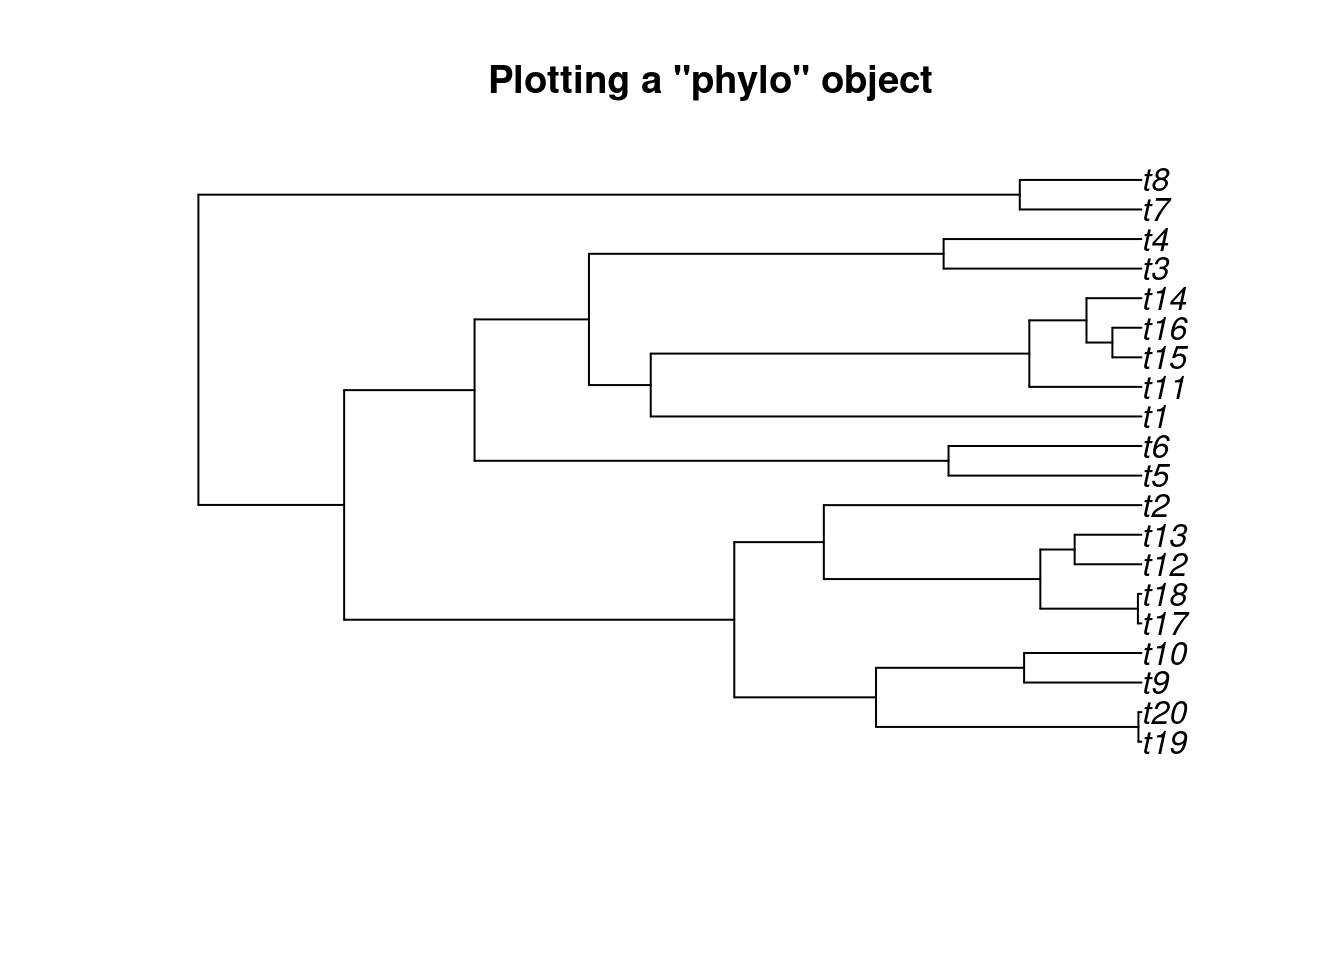
\includegraphics{treats_manual_files/figure-latex/unnamed-chunk-104-1.pdf}

However, if you also simulated a trait along with the tree you can use the \texttt{plot.treats} function to plot both the tree and the trait:

\begin{Shaded}
\begin{Highlighting}[]
\CommentTok{\#\# A simple pure birth tree with a BM process}
\NormalTok{my\_tree \textless{}{-}}\StringTok{ }\KeywordTok{treats}\NormalTok{(}\DataTypeTok{stop.rule =} \KeywordTok{list}\NormalTok{(}\DataTypeTok{max.taxa =} \DecValTok{20}\NormalTok{), }\DataTypeTok{traits =} \KeywordTok{make.traits}\NormalTok{())}
\CommentTok{\#\# Playing with the default options}
\KeywordTok{plot}\NormalTok{(my\_tree, }\DataTypeTok{main =} \StringTok{"A tree and traits"}\NormalTok{)}
\end{Highlighting}
\end{Shaded}

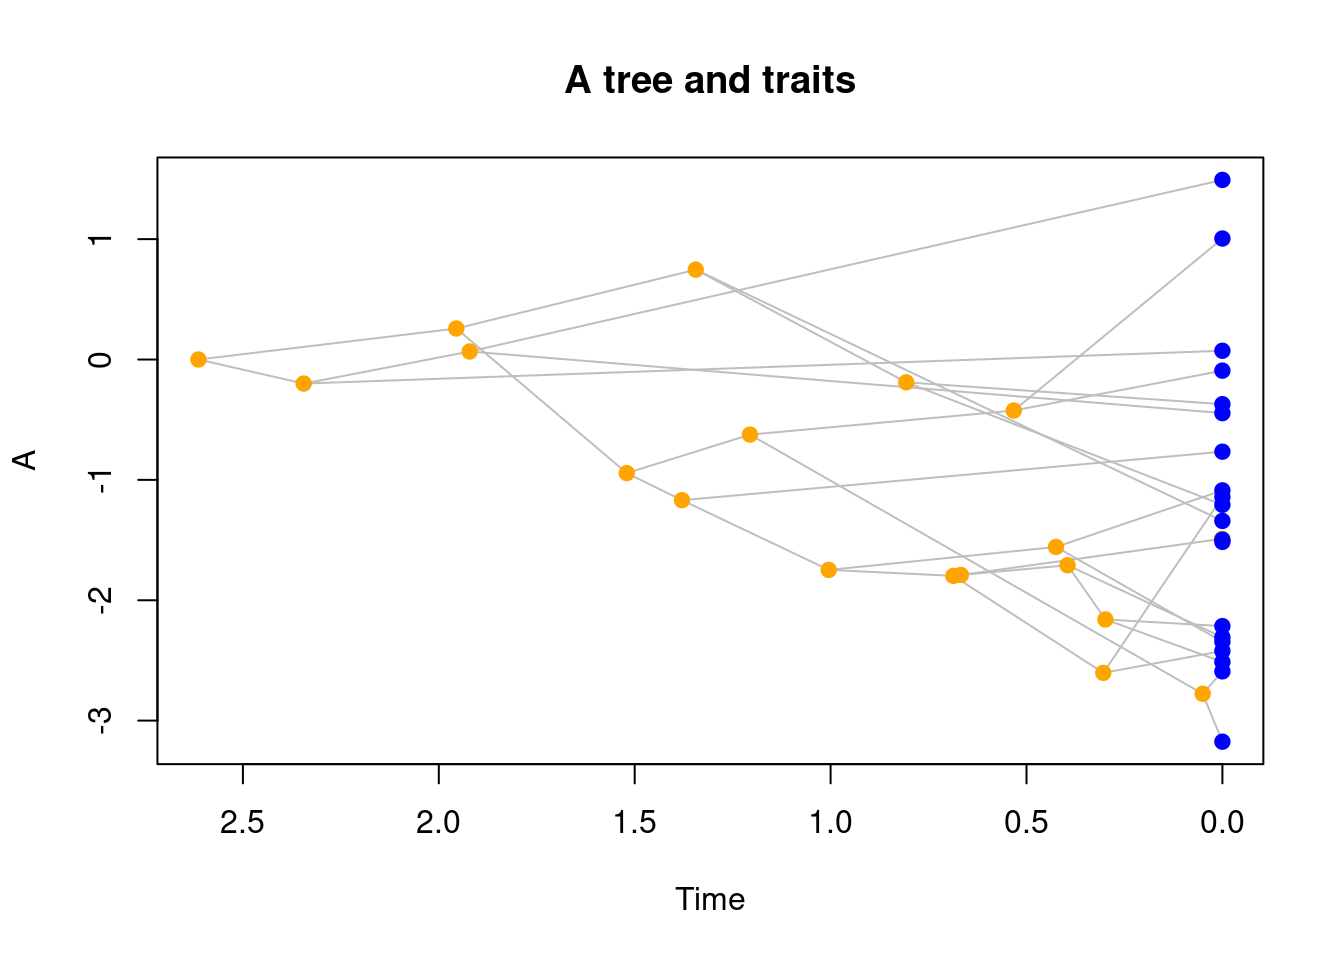
\includegraphics{treats_manual_files/figure-latex/unnamed-chunk-105-1.pdf}

By default, elements are coloured as follows: nodes and tips are points and coloured in blue if they are tips (light blue if they are fossils) and nodes are in orange.
Branches linking them are grey lines.
You can of course change this colour palette to whatever you prefer by calling the standard base R arguments that can be passed to \texttt{points} or \texttt{lines}. For example \texttt{pch} for the point type or \texttt{lty} for the line type.
Furthermore, time is plotted conventionally from left to right (left is towards the past, right is towards the present) but you can change that by specifying \texttt{xlim}.

\begin{Shaded}
\begin{Highlighting}[]
\CommentTok{\#\# Playing with some more options}
\KeywordTok{plot}\NormalTok{(my\_tree, }\DataTypeTok{main =} \StringTok{"A tree and traits"}\NormalTok{,}
     \CommentTok{\#\# Changing nodes colours and type}
     \DataTypeTok{col =} \KeywordTok{c}\NormalTok{(}\DataTypeTok{tips =} \StringTok{"pink"}\NormalTok{, }\DataTypeTok{nodes =} \StringTok{"purple"}\NormalTok{), }\DataTypeTok{pch =} \DecValTok{21}\NormalTok{,}
     \CommentTok{\#\# Changing edge colour and type}
     \DataTypeTok{lwd =} \DecValTok{2}\NormalTok{, }\DataTypeTok{lty =} \DecValTok{3}\NormalTok{, }\DataTypeTok{edges =} \StringTok{"yellow"}\NormalTok{,}
     \CommentTok{\#\# Changing the x axis orientation and label}
     \DataTypeTok{xlim =} \KeywordTok{c}\NormalTok{(}\DecValTok{0}\NormalTok{, }\FloatTok{2.5}\NormalTok{), }\DataTypeTok{xlab =} \StringTok{"Time into the past"}\NormalTok{)}
\end{Highlighting}
\end{Shaded}

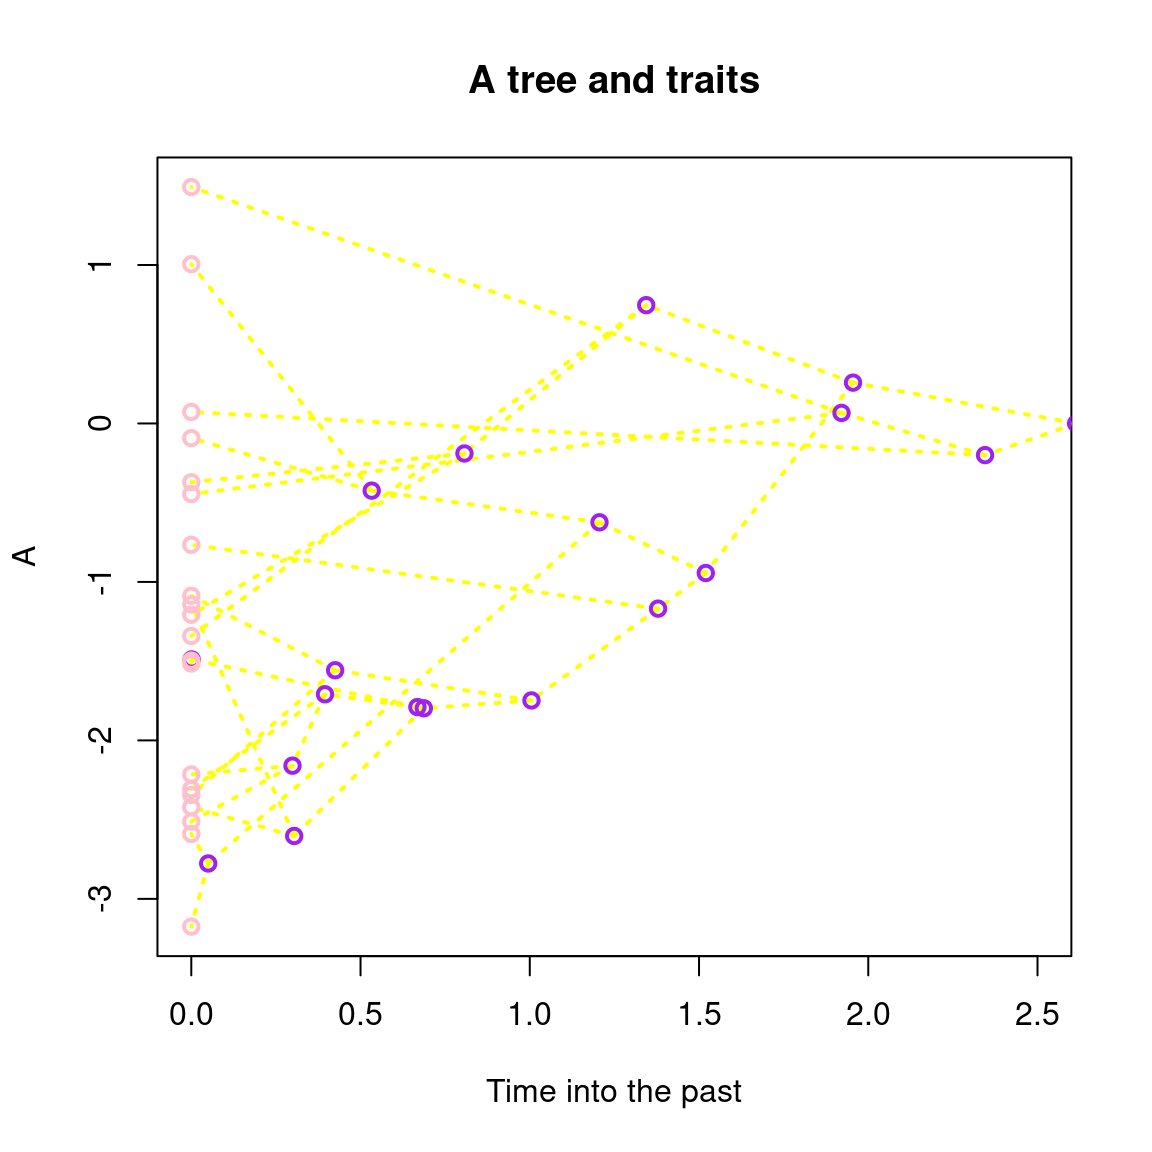
\includegraphics{treats_manual_files/figure-latex/unnamed-chunk-106-1.pdf}

\begin{quote}
Note that in \texttt{plot.treats} you can modify colours using the \texttt{col} argument by providing a clear indication of what you want to colour (e.g.~\texttt{col\ =\ c(tips\ =\ "blue",\ fossils\ =\ "orange")} will apply the colours to the unambiguously named elements) or by providing a function that will scale the colours with time (e.g.~\texttt{col\ =\ grDevices::heat.colors} will use the specified function to change the colours of the elements through time).
\end{quote}

You can add a default legend by using \texttt{legend\ =\ TRUE} (if you don't want to add the default legend you can add it after your plot using \texttt{legend(...)}).

\begin{Shaded}
\begin{Highlighting}[]
\CommentTok{\#\# Adding the default legend}
\KeywordTok{plot}\NormalTok{(my\_tree, }\DataTypeTok{legend =} \OtherTok{TRUE}\NormalTok{)}
\end{Highlighting}
\end{Shaded}

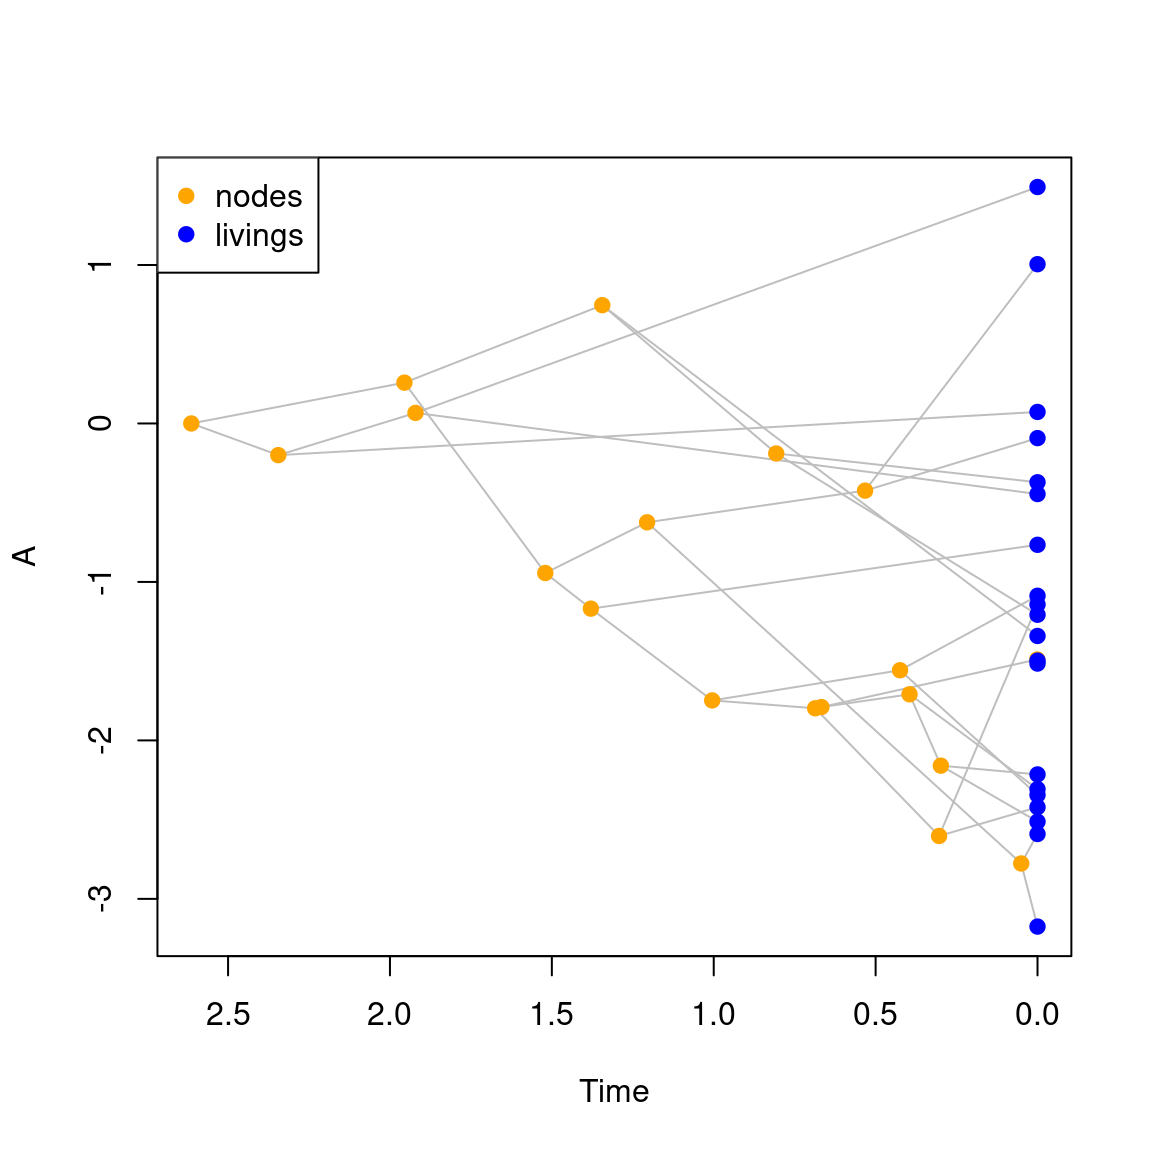
\includegraphics{treats_manual_files/figure-latex/unnamed-chunk-107-1.pdf}

\hypertarget{adding-dimensions-not-necessary-but-fun}{%
\subsection{Adding dimensions! Not necessary, but fun!}\label{adding-dimensions-not-necessary-but-fun}}

Of course, if you're simulating multiple traits, you can always plot different ones.

\begin{Shaded}
\begin{Highlighting}[]
\CommentTok{\#\# Specifying a 3D trait process}
\NormalTok{my\_3D\_trait \textless{}{-}}\StringTok{ }\KeywordTok{make.traits}\NormalTok{(}\DataTypeTok{n =} \DecValTok{3}\NormalTok{, )}
\CommentTok{\#\# Simulating a birth{-}death tree with that 3D trait}
\NormalTok{my\_data \textless{}{-}}\StringTok{ }\KeywordTok{treats}\NormalTok{(}\DataTypeTok{bd.params =} \KeywordTok{list}\NormalTok{(}\DataTypeTok{extinction =} \FloatTok{0.2}\NormalTok{),}
                \DataTypeTok{stop.rule =} \KeywordTok{list}\NormalTok{(}\DataTypeTok{max.living =} \DecValTok{50}\NormalTok{),}
                \DataTypeTok{traits    =}\NormalTok{ my\_3D\_trait)}
\end{Highlighting}
\end{Shaded}

You can toggle which trait to plot using the \texttt{trait} option, either by providing a single value to plot that specific trait against time or by providing two traits.

\begin{Shaded}
\begin{Highlighting}[]
\KeywordTok{par}\NormalTok{(}\DataTypeTok{mfrow =} \KeywordTok{c}\NormalTok{(}\DecValTok{2}\NormalTok{,}\DecValTok{1}\NormalTok{))}
\CommentTok{\#\# Plotting the second trait}
\KeywordTok{plot}\NormalTok{(my\_data, }\DataTypeTok{trait =} \DecValTok{2}\NormalTok{, }\DataTypeTok{main =} \StringTok{"Trait 2"}\NormalTok{)}
\CommentTok{\#\# Plotting the correlation between trait 1 and 2}
\KeywordTok{plot}\NormalTok{(my\_data, }\DataTypeTok{trait =} \KeywordTok{c}\NormalTok{(}\DecValTok{1}\NormalTok{,}\DecValTok{2}\NormalTok{), }\DataTypeTok{main =} \StringTok{"Traits 1 and 2"}\NormalTok{)}
\end{Highlighting}
\end{Shaded}

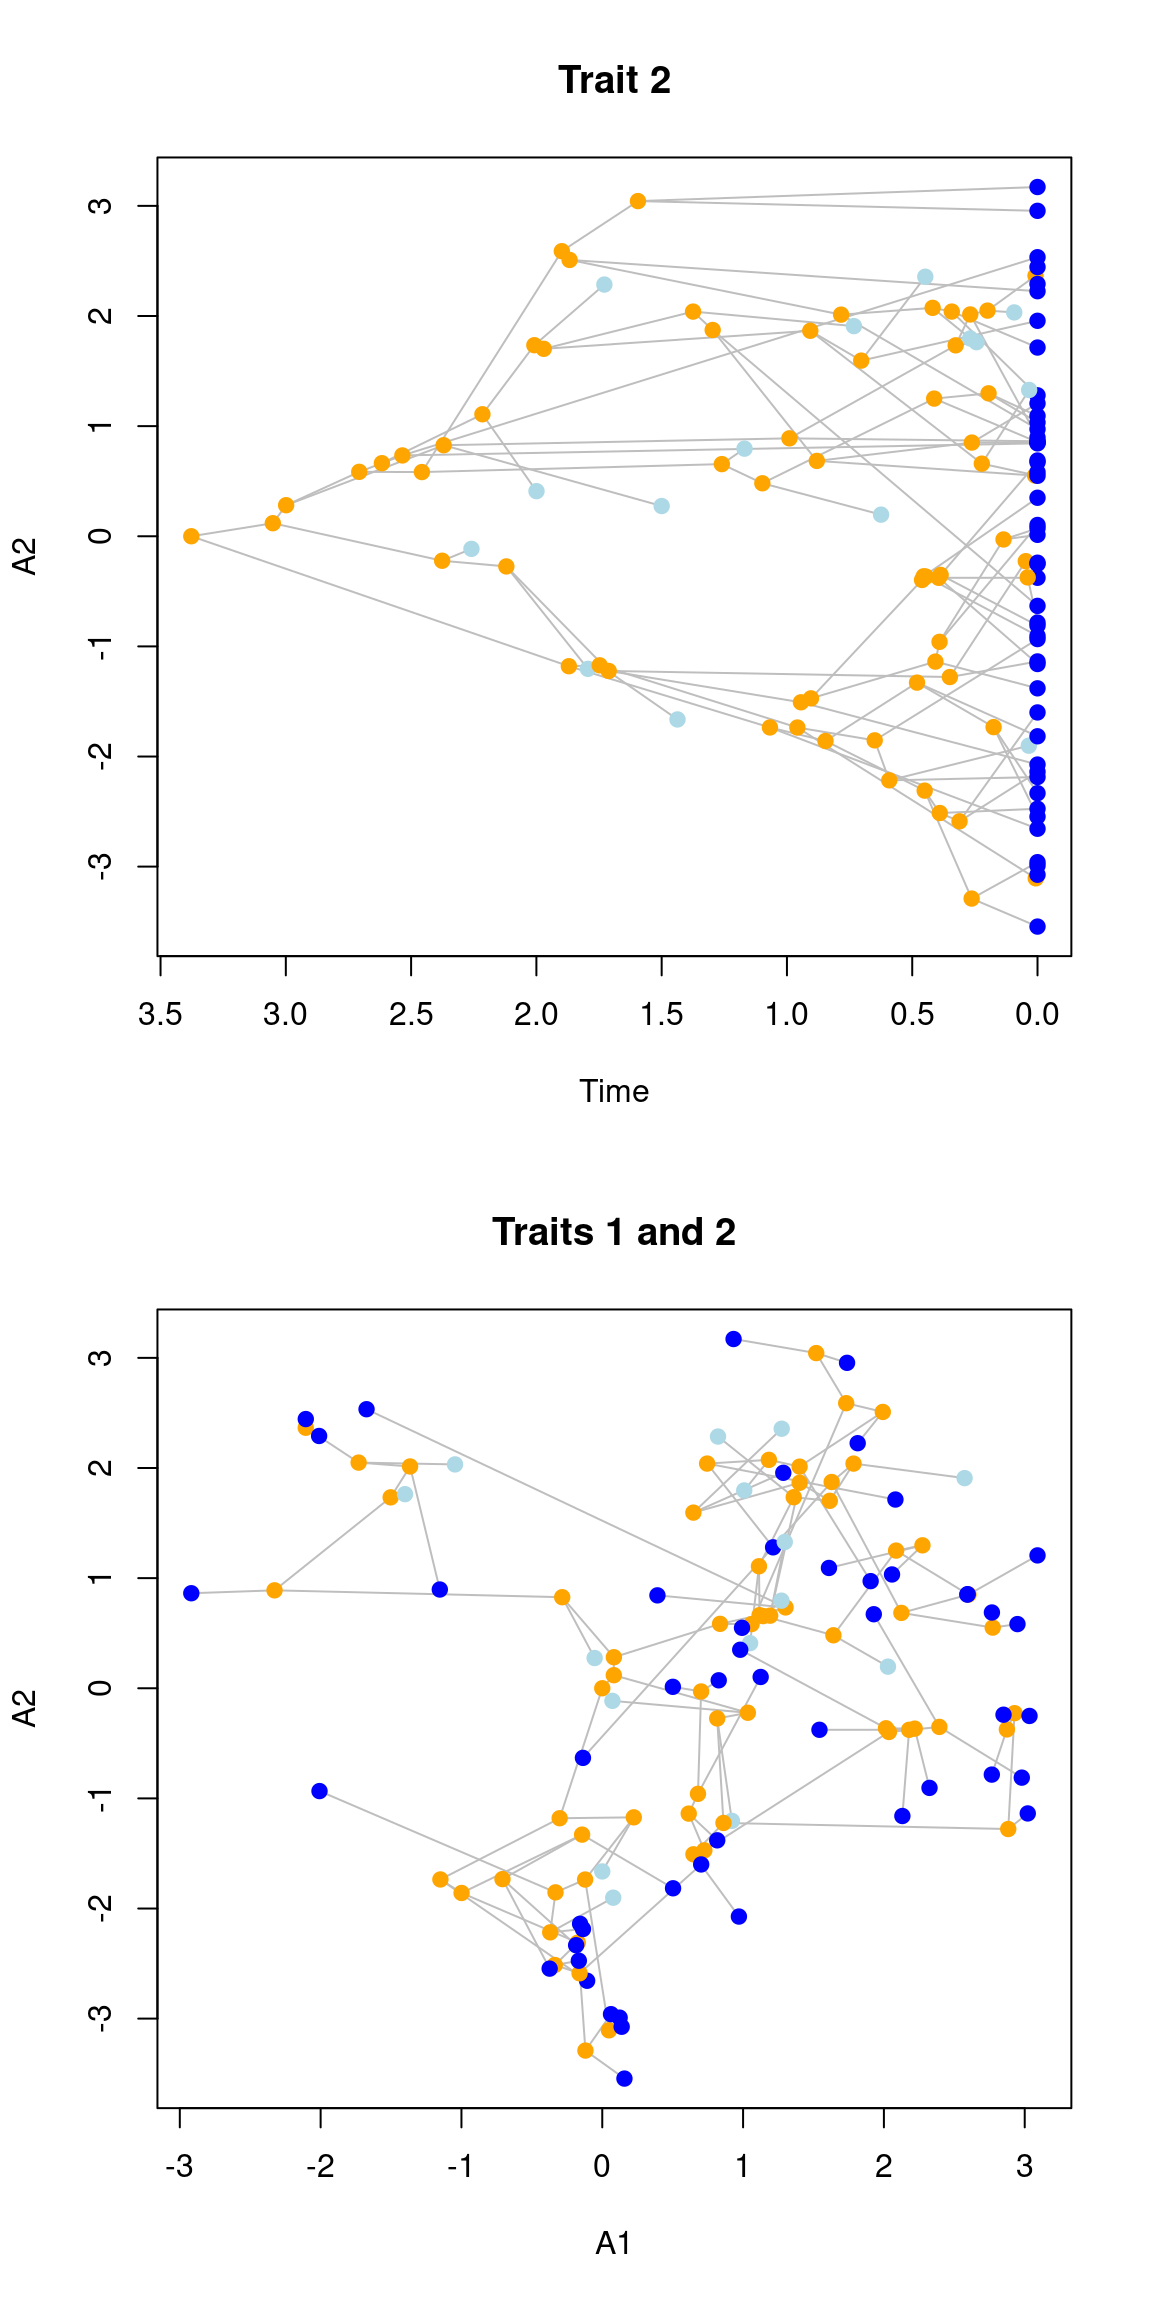
\includegraphics{treats_manual_files/figure-latex/unnamed-chunk-109-1.pdf}

As mentioned above, the \texttt{col} argument can take a function for scaling the elements colours with time.
This can be useful for adding time a third dimension to these 2D plots:

\begin{Shaded}
\begin{Highlighting}[]
\CommentTok{\#\# Plotting the correlation between trait 1 and 2}
\CommentTok{\#\# with time as a 3rd dimensions}
\KeywordTok{plot}\NormalTok{(my\_data, }\DataTypeTok{trait =} \KeywordTok{c}\NormalTok{(}\DecValTok{1}\NormalTok{,}\DecValTok{2}\NormalTok{), }\DataTypeTok{main =} \StringTok{"Traits 1 and 2"}\NormalTok{,}
     \DataTypeTok{col =}\NormalTok{ grDevices}\OperatorTok{::}\NormalTok{heat.colors, }\DataTypeTok{legend =} \OtherTok{TRUE}\NormalTok{,}
     \CommentTok{\#\# Highlighting the tips in black for visibility}
     \DataTypeTok{tips.nodes =} \StringTok{"black"}\NormalTok{)}
\end{Highlighting}
\end{Shaded}

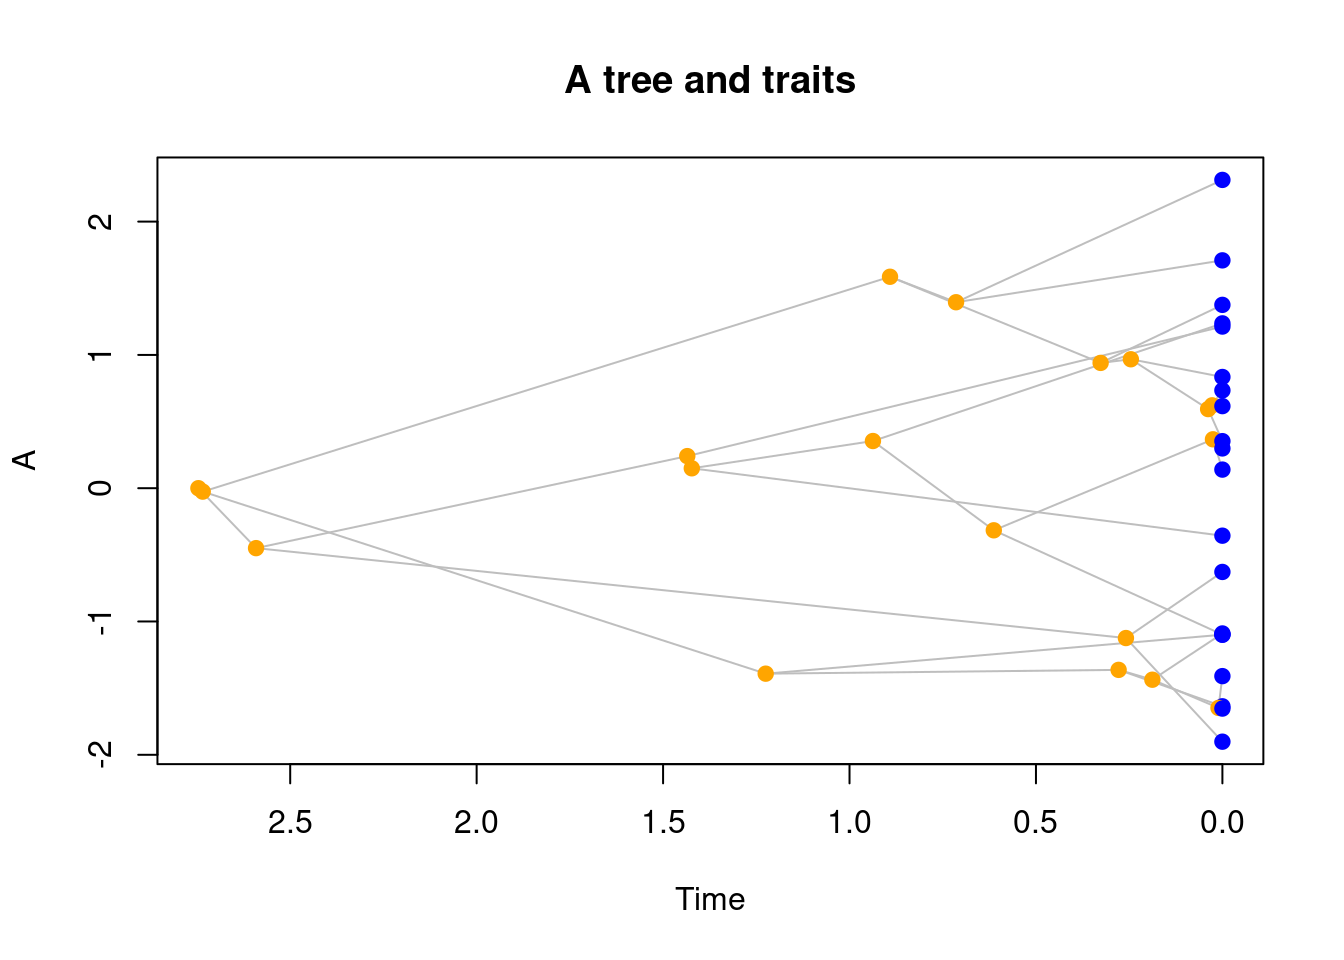
\includegraphics{treats_manual_files/figure-latex/unnamed-chunk-110-1.pdf}

But there's more! You can also plot these results using actual 3D plots that you can spin and all that!
This is done through the \texttt{rgl} package and activated in \texttt{treats} using the option \texttt{use.3D\ =\ TRUE}.

If two traits are provided, the 3rd dimension is going to be time by default:

\begin{Shaded}
\begin{Highlighting}[]
\CommentTok{\#\# Plotting the tree and 2 traits in 3D: woah!}
\KeywordTok{plot}\NormalTok{(my\_data, }\DataTypeTok{trait =} \KeywordTok{c}\NormalTok{(}\DecValTok{1}\NormalTok{, }\DecValTok{2}\NormalTok{), }\DataTypeTok{use.3D =} \OtherTok{TRUE}\NormalTok{)}
\KeywordTok{rglwidget}\NormalTok{()}
\end{Highlighting}
\end{Shaded}

\begin{verbatim}
## Warning in snapshot3d(scene = x, width = width, height = height): webshot =
## TRUE requires the webshot2 package and Chrome browser; using rgl.snapshot()
## instead
\end{verbatim}

\begin{verbatim}
## Warning in rgl.snapshot(filename, fmt, top): this build of rgl does not support
## snapshots
\end{verbatim}

\includegraphics[width=6.5in]{../../../../../../tmp/RtmpcKuqE6/file37eb79e5b154}

If three traits are provide, you can set up a fourth coloured dimension as time (similarly to the 2D plots with the colour gradients).
This uses the \texttt{rgl} functions, namely \texttt{lines3d}, \texttt{points3d} (if \texttt{type\ =\ "p"}; default) or \texttt{sphere3d} (if \texttt{type\ =\ "s"}).
The additional arguments \texttt{...} are directly handled and attributed to the corresponding function.

\begin{Shaded}
\begin{Highlighting}[]
\CommentTok{\#\# Plotting the tree and 3 traits in 3D}
\KeywordTok{plot}\NormalTok{(my\_data, }\DataTypeTok{trait =} \KeywordTok{c}\NormalTok{(}\DecValTok{1}\NormalTok{, }\DecValTok{2}\NormalTok{, }\DecValTok{3}\NormalTok{), }\DataTypeTok{use.3D =} \OtherTok{TRUE}\NormalTok{,}
     \DataTypeTok{col =}\NormalTok{ grDevices}\OperatorTok{::}\NormalTok{heat.colors, }\DataTypeTok{type =} \StringTok{"s"}\NormalTok{, }\DataTypeTok{radius =} \FloatTok{0.1}\NormalTok{)}
\KeywordTok{rglwidget}\NormalTok{()}
\end{Highlighting}
\end{Shaded}

\begin{verbatim}
## Warning in snapshot3d(scene = x, width = width, height = height): webshot =
## TRUE requires the webshot2 package and Chrome browser; using rgl.snapshot()
## instead
\end{verbatim}

\begin{verbatim}
## Warning in rgl.snapshot(filename, fmt, top): this build of rgl does not support
## snapshots
\end{verbatim}

\includegraphics[width=6.5in]{../../../../../../tmp/RtmpcKuqE6/file37eb42b1cdb9}

\hypertarget{specific-examples}{%
\chapter{Specific examples}\label{specific-examples}}

In this section I will illustrate a series of examples of specific more complex scenarios.
They can be all run independently and used as a basis for your own specific scenarios.

Here is a table summarising which functionalities are used in which example:

\begin{longtable}[]{@{}ll@{}}
\toprule
\begin{minipage}[b]{0.57\columnwidth}\raggedright
Functionality showcase\strut
\end{minipage} & \begin{minipage}[b]{0.37\columnwidth}\raggedright
Example\strut
\end{minipage}\tabularnewline
\midrule
\endhead
\begin{minipage}[t]{0.57\columnwidth}\raggedright
\texttt{bd.params}\strut
\end{minipage} & \begin{minipage}[t]{0.37\columnwidth}\raggedright
\protect\hyperlink{EGred_spec}{reducing speciation rate}, \protect\hyperlink{EG_founding_purebirth}{generating a subtree with no extinction}\strut
\end{minipage}\tabularnewline
\begin{minipage}[t]{0.57\columnwidth}\raggedright
\texttt{make.events}\strut
\end{minipage} & \begin{minipage}[t]{0.37\columnwidth}\raggedright
\protect\hyperlink{EGrandom_ext}{mass extinction}, \protect\hyperlink{EGneg_ext}{negative trait extinction}, \protect\hyperlink{EGbg_ext}{background extinction}, \protect\hyperlink{EGred_spec}{reducing speciation rate}, \protect\hyperlink{EG_change_trait}{changing trait process}, \protect\hyperlink{EG_change_correlation}{changing trait correlation}, \protect\hyperlink{EG_change_modif}{changing modifiers}, \protect\hyperlink{EG_modify_brlen}{change branch length}, \protect\hyperlink{EG_founding_purebirth}{generating a subtree with no extinction}, \href{EG_founding_traits}{generating a subtree with a different process}\strut
\end{minipage}\tabularnewline
\begin{minipage}[t]{0.57\columnwidth}\raggedright
\texttt{make.traits}\strut
\end{minipage} & \begin{minipage}[t]{0.37\columnwidth}\raggedright
\protect\hyperlink{EGneg_ext}{negative trait extinction}, \protect\hyperlink{EG_change_trait}{changing trait process}, \protect\hyperlink{EG_change_correlation}{changing trait correlation}, \href{EG_founding_traits}{generating a subtree with a different process}\strut
\end{minipage}\tabularnewline
\begin{minipage}[t]{0.57\columnwidth}\raggedright
\texttt{make.modifiers}\strut
\end{minipage} & \begin{minipage}[t]{0.37\columnwidth}\raggedright
\protect\hyperlink{EG_change_modif}{changing modifiers}, \protect\hyperlink{EG_modify_brlen}{change branch length}\strut
\end{minipage}\tabularnewline
\bottomrule
\end{longtable}

And more specifically for the events:

\begin{longtable}[]{@{}ll@{}}
\toprule
\begin{minipage}[b]{0.55\columnwidth}\raggedright
Functionality showcase\strut
\end{minipage} & \begin{minipage}[b]{0.39\columnwidth}\raggedright
Example\strut
\end{minipage}\tabularnewline
\midrule
\endhead
\begin{minipage}[t]{0.55\columnwidth}\raggedright
\texttt{age.condition}\strut
\end{minipage} & \begin{minipage}[t]{0.39\columnwidth}\raggedright
\protect\hyperlink{EGrandom_ext}{mass extinction}, \protect\hyperlink{EGneg_ext}{negative trait extinction}, \protect\hyperlink{EGred_spec}{reducing speciation rate}, \protect\hyperlink{EG_change_trait}{changing trait process}, \protect\hyperlink{EG_change_modif}{changing modifiers}\strut
\end{minipage}\tabularnewline
\begin{minipage}[t]{0.55\columnwidth}\raggedright
\texttt{random.extinction}\strut
\end{minipage} & \begin{minipage}[t]{0.39\columnwidth}\raggedright
\protect\hyperlink{EGrandom_ext}{mass extinction}\strut
\end{minipage}\tabularnewline
\begin{minipage}[t]{0.55\columnwidth}\raggedright
\texttt{trait.extinction}\strut
\end{minipage} & \begin{minipage}[t]{0.39\columnwidth}\raggedright
\protect\hyperlink{EGneg_ext}{negative trait extinction}\strut
\end{minipage}\tabularnewline
\begin{minipage}[t]{0.55\columnwidth}\raggedright
\texttt{taxa.condition}\strut
\end{minipage} & \begin{minipage}[t]{0.39\columnwidth}\raggedright
\protect\hyperlink{EGbg_ext}{background extinction}, \protect\hyperlink{EG_modify_brlen}{change branch length}\strut
\end{minipage}\tabularnewline
\begin{minipage}[t]{0.55\columnwidth}\raggedright
\texttt{bd.params.update}\strut
\end{minipage} & \begin{minipage}[t]{0.39\columnwidth}\raggedright
\protect\hyperlink{EGbg_ext}{background extinction}, \protect\hyperlink{EGred_spec}{reducing speciation rate}\strut
\end{minipage}\tabularnewline
\begin{minipage}[t]{0.55\columnwidth}\raggedright
\texttt{traits.update}\strut
\end{minipage} & \begin{minipage}[t]{0.39\columnwidth}\raggedright
\protect\hyperlink{EG_change_trait}{changing trait process}, \protect\hyperlink{EG_change_correlation}{changing trait correlation}\strut
\end{minipage}\tabularnewline
\begin{minipage}[t]{0.55\columnwidth}\raggedright
\texttt{trait.condition}\strut
\end{minipage} & \begin{minipage}[t]{0.39\columnwidth}\raggedright
\protect\hyperlink{EG_change_correlation}{changing trait correlation}, \href{EG_founding_traits}{generating a subtree with a different process}\strut
\end{minipage}\tabularnewline
\begin{minipage}[t]{0.55\columnwidth}\raggedright
\texttt{modifiers.update}\strut
\end{minipage} & \begin{minipage}[t]{0.39\columnwidth}\raggedright
\protect\hyperlink{EG_change_modif}{changing modifiers}, \protect\hyperlink{EG_modify_brlen}{change branch length}\strut
\end{minipage}\tabularnewline
\begin{minipage}[t]{0.55\columnwidth}\raggedright
\texttt{parent.traits}\strut
\end{minipage} & \begin{minipage}[t]{0.39\columnwidth}\raggedright
\protect\hyperlink{EG_change_modif}{changing modifiers}\strut
\end{minipage}\tabularnewline
\begin{minipage}[t]{0.55\columnwidth}\raggedright
\texttt{founding.event}\strut
\end{minipage} & \begin{minipage}[t]{0.39\columnwidth}\raggedright
\protect\hyperlink{EG_founding_purebirth}{generating a subtree with no extinction}, \href{EG_founding_traits}{generating a subtree with a different process}\strut
\end{minipage}\tabularnewline
\bottomrule
\end{longtable}

\hypertarget{EGrandom_ext}{%
\section{Random mass extinction after some time}\label{EGrandom_ext}}

For this scenario, we want to generate a pure birth tree (no traits and no extinction) where 80\% of the species go extinct two thirds of the way into the scenario.

For that we first need to first set our simulation parameters: we will be running the simulation for 6 time units and with a speciation rate of 1 (and extinction of 0 - default).

\begin{Shaded}
\begin{Highlighting}[]
\CommentTok{\#\# Setting the parameters}
\NormalTok{stop\_time\_}\DecValTok{6}\NormalTok{ \textless{}{-}}\StringTok{ }\KeywordTok{list}\NormalTok{(}\DataTypeTok{max.time =} \DecValTok{6}\NormalTok{)}
\NormalTok{speciation\_}\DecValTok{1}\NormalTok{ \textless{}{-}}\StringTok{ }\KeywordTok{make.bd.params}\NormalTok{(}\DataTypeTok{speciation =} \DecValTok{1}\NormalTok{)}
\end{Highlighting}
\end{Shaded}

We will then create a event that triggers when reaching half of the simulation time (using \texttt{age.condition(2.5)}).
This event will target \texttt{"taxa"}, i.e.~the number of species, and randomly remove 80\% of them (using \texttt{random.extinction(0.8)}):

\begin{Shaded}
\begin{Highlighting}[]
\CommentTok{\#\# 80\% mass extinction at time 4}
\NormalTok{mass.extinction \textless{}{-}}\StringTok{ }\KeywordTok{make.events}\NormalTok{(}
                    \DataTypeTok{condition =} \KeywordTok{age.condition}\NormalTok{(}\DecValTok{4}\NormalTok{),}
                    \DataTypeTok{target =} \StringTok{"taxa"}\NormalTok{,}
                    \DataTypeTok{modification =} \KeywordTok{random.extinction}\NormalTok{(}\FloatTok{0.8}\NormalTok{))}
\end{Highlighting}
\end{Shaded}

Once these parameters are defined, we can run the simulations and plot the results:

\begin{Shaded}
\begin{Highlighting}[]
\CommentTok{\#\# Running the simulations}
\KeywordTok{set.seed}\NormalTok{(}\DecValTok{1}\NormalTok{)}
\NormalTok{results \textless{}{-}}\StringTok{ }\KeywordTok{treats}\NormalTok{(}\DataTypeTok{stop.rule =}\NormalTok{ stop\_time\_}\DecValTok{6}\NormalTok{,}
                \DataTypeTok{bd.params =}\NormalTok{ speciation\_}\DecValTok{1}\NormalTok{,}
                \DataTypeTok{events    =}\NormalTok{ mass.extinction)}
\CommentTok{\#\# Plotting the results}
\KeywordTok{plot}\NormalTok{(results, }\DataTypeTok{show.tip.label =} \OtherTok{FALSE}\NormalTok{)}
\KeywordTok{axisPhylo}\NormalTok{()}
\end{Highlighting}
\end{Shaded}

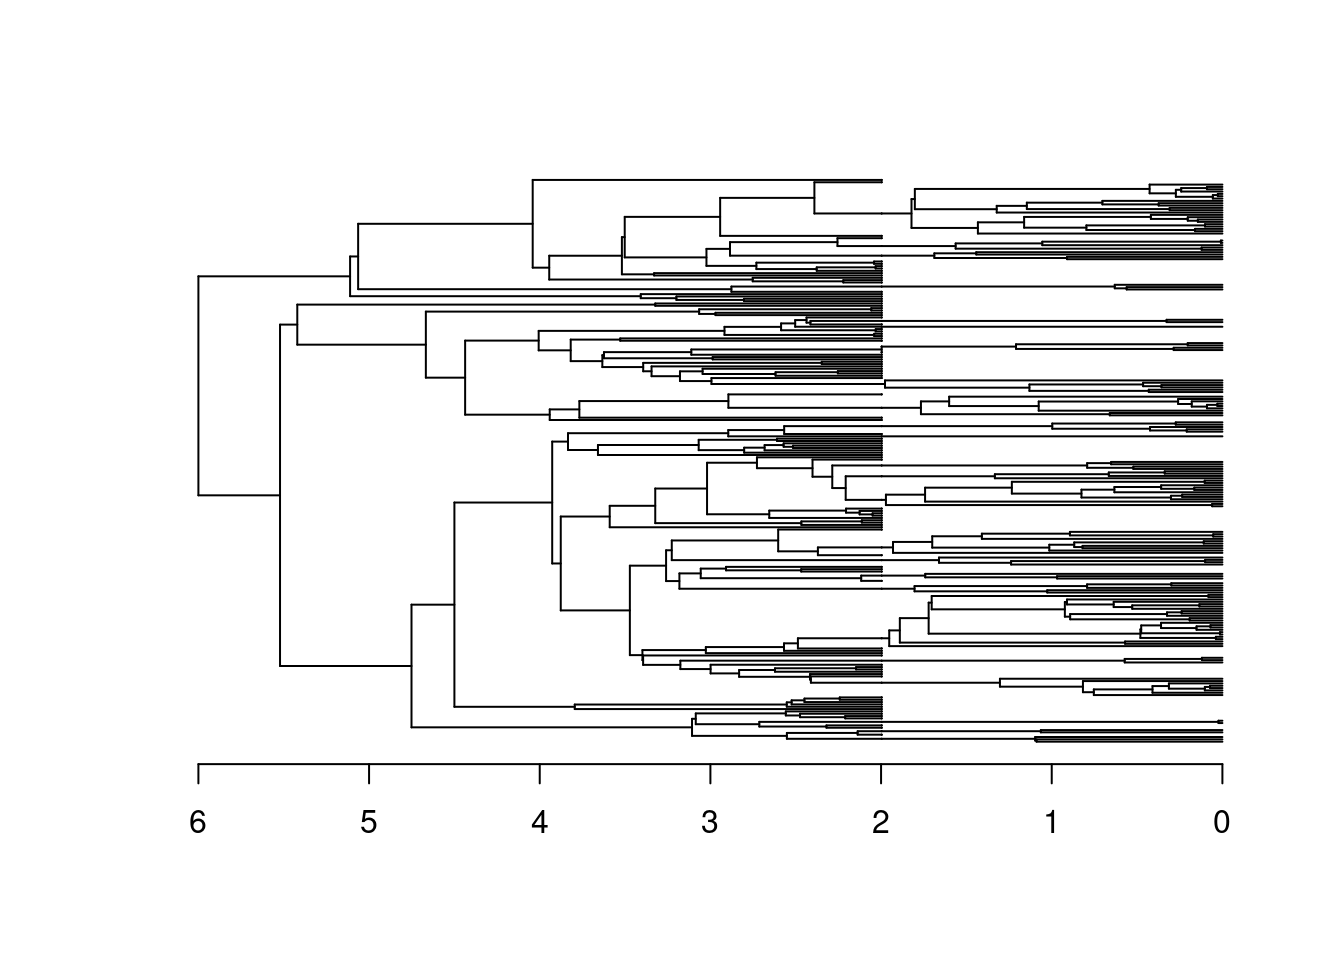
\includegraphics{treats_manual_files/figure-latex/unnamed-chunk-116-1.pdf}

\hypertarget{EGneg_ext}{%
\section{Species with negative trait values go extinct after a certain time}\label{EGneg_ext}}

For this scenario, we want to generate a pure birth tree with a one dimensional Brownian Motion trait for 5 time units.
We then want species with a negative trait value go extinct after 4 time units.

First we need to set up the simulation parameters:
* The stopping rule (5 time units)
* The birth-death parameters (speciation rate of 1)

\begin{Shaded}
\begin{Highlighting}[]
\CommentTok{\#\# Simulation parameters}
\NormalTok{stop\_time\_}\DecValTok{5}\NormalTok{ \textless{}{-}}\StringTok{ }\KeywordTok{list}\NormalTok{(}\DataTypeTok{max.time =} \DecValTok{5}\NormalTok{)}
\NormalTok{speciation\_}\DecValTok{1}\NormalTok{ \textless{}{-}}\StringTok{ }\KeywordTok{make.bd.params}\NormalTok{(}\DataTypeTok{speciation =} \DecValTok{1}\NormalTok{)}
\end{Highlighting}
\end{Shaded}

Then set up our trait which is a one dimensional Brownian Motion

\begin{Shaded}
\begin{Highlighting}[]
\CommentTok{\#\# Trait}
\NormalTok{simple\_bm\_trait \textless{}{-}}\StringTok{ }\KeywordTok{make.traits}\NormalTok{(}\DataTypeTok{n =} \DecValTok{1}\NormalTok{, }\DataTypeTok{process =}\NormalTok{ BM.process)}
\end{Highlighting}
\end{Shaded}

And our extinction event which triggers after reaching time 4 (\texttt{age.condition(4)}), targets the \texttt{"taxa"} and modifies the extinction for species with traits lower than 0.

\begin{Shaded}
\begin{Highlighting}[]
\CommentTok{\#\# Extinction of any tips with trait \textless{} 1 at time 4}
\NormalTok{trait.extinction \textless{}{-}}\StringTok{ }\KeywordTok{make.events}\NormalTok{(}
                      \DataTypeTok{target =} \StringTok{"taxa"}\NormalTok{,}
                      \DataTypeTok{condition =} \KeywordTok{age.condition}\NormalTok{(}\DecValTok{4}\NormalTok{),}
                      \DataTypeTok{modification =} \KeywordTok{trait.extinction}\NormalTok{(}\DataTypeTok{x =} \DecValTok{0}\NormalTok{,}
                                                      \DataTypeTok{condition =} \StringTok{\textasciigrave{}}\DataTypeTok{\textless{}}\StringTok{\textasciigrave{}}\NormalTok{))}
\end{Highlighting}
\end{Shaded}

Once these parameters are defined, we can run the simulations and plot the results:

\begin{Shaded}
\begin{Highlighting}[]
\CommentTok{\#\# Running the simulations}
\KeywordTok{set.seed}\NormalTok{(}\DecValTok{7}\NormalTok{)}
\NormalTok{results \textless{}{-}}\StringTok{ }\KeywordTok{treats}\NormalTok{(}\DataTypeTok{stop.rule =}\NormalTok{ stop\_time\_}\DecValTok{5}\NormalTok{,}
                \DataTypeTok{bd.params =}\NormalTok{ speciation\_}\DecValTok{1}\NormalTok{,}
                \DataTypeTok{traits    =}\NormalTok{ simple\_bm\_trait,}
                \DataTypeTok{events    =}\NormalTok{ trait.extinction)}
\CommentTok{\#\# Plotting the results}
\KeywordTok{plot}\NormalTok{(results)}
\end{Highlighting}
\end{Shaded}

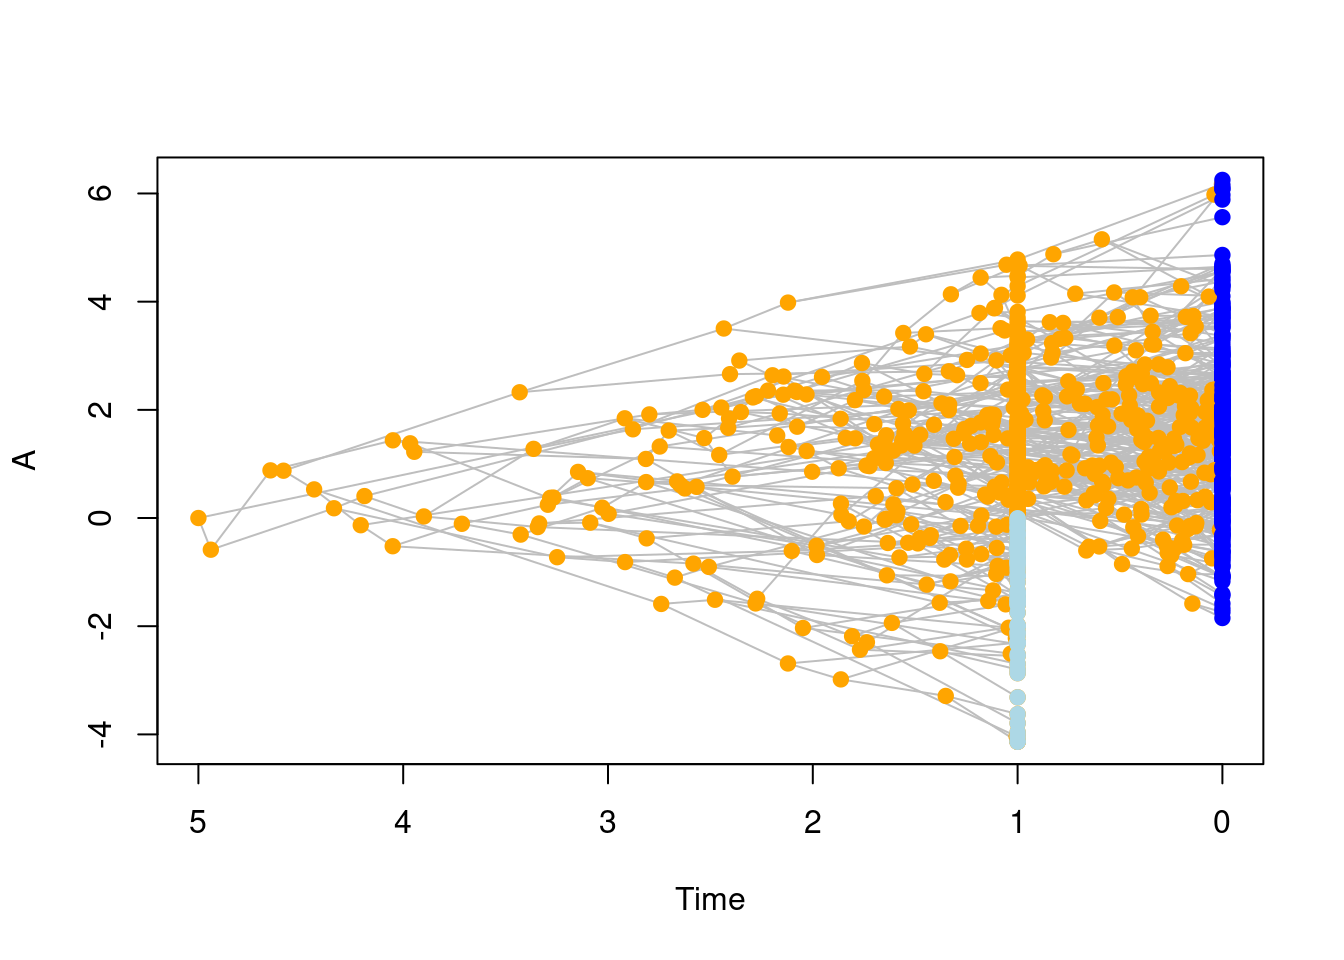
\includegraphics{treats_manual_files/figure-latex/unnamed-chunk-120-1.pdf}

\hypertarget{EGbg_ext}{%
\section{Adding a background extinction after reaching a number of living taxa}\label{EGbg_ext}}

For this scenario, we want to generate a pure birth tree until reaching 50 living taxa but with an extinction rate appearing after reaching 30 taxa.

First we need to set up the simulation parameters:
* The stopping rule (50 taxa max)
* The birth-death parameters (speciation rate of 1)

\begin{Shaded}
\begin{Highlighting}[]
\CommentTok{\#\# Simulation parameters}
\NormalTok{stop\_taxa\_}\DecValTok{50}\NormalTok{ \textless{}{-}}\StringTok{ }\KeywordTok{list}\NormalTok{(}\DataTypeTok{max.living =} \DecValTok{50}\NormalTok{)}
\NormalTok{speciation\_}\DecValTok{1}\NormalTok{ \textless{}{-}}\StringTok{ }\KeywordTok{make.bd.params}\NormalTok{(}\DataTypeTok{speciation =} \DecValTok{1}\NormalTok{)}
\end{Highlighting}
\end{Shaded}

And our change in extinction rate event which triggers after reaching 30 taxa (\texttt{taxa.condition(30)}), targets the \texttt{"bd.params"} (birth-death parameters) sets the extinction rate to 0.5 (\texttt{bd.params.update(extinction\ =\ 0.5)}):

\begin{Shaded}
\begin{Highlighting}[]
\CommentTok{\#\# Adding an extinction parameter after 30 taxa}
\NormalTok{background.extinction \textless{}{-}}\StringTok{ }\KeywordTok{make.events}\NormalTok{(}
                      \DataTypeTok{condition =} \KeywordTok{taxa.condition}\NormalTok{(}\DecValTok{30}\NormalTok{),}
                      \DataTypeTok{target =} \StringTok{"bd.params"}\NormalTok{,}
                      \DataTypeTok{modification =} \KeywordTok{bd.params.update}\NormalTok{(}\DataTypeTok{extinction =} \FloatTok{0.5}\NormalTok{))}
\end{Highlighting}
\end{Shaded}

Once these parameters are defined, we can run the simulations and plot the results:

\begin{Shaded}
\begin{Highlighting}[]
\CommentTok{\#\# Running the simulations}
\KeywordTok{set.seed}\NormalTok{(}\DecValTok{2}\NormalTok{)}
\NormalTok{results \textless{}{-}}\StringTok{ }\KeywordTok{treats}\NormalTok{(}\DataTypeTok{stop.rule =}\NormalTok{ stop\_taxa\_}\DecValTok{50}\NormalTok{,}
                \DataTypeTok{bd.params =}\NormalTok{ speciation\_}\DecValTok{1}\NormalTok{,}
                \DataTypeTok{events =}\NormalTok{ background.extinction)}
\CommentTok{\#\# Plotting the results}
\KeywordTok{plot}\NormalTok{(results, }\DataTypeTok{show.tip.label =} \OtherTok{FALSE}\NormalTok{)}
\end{Highlighting}
\end{Shaded}

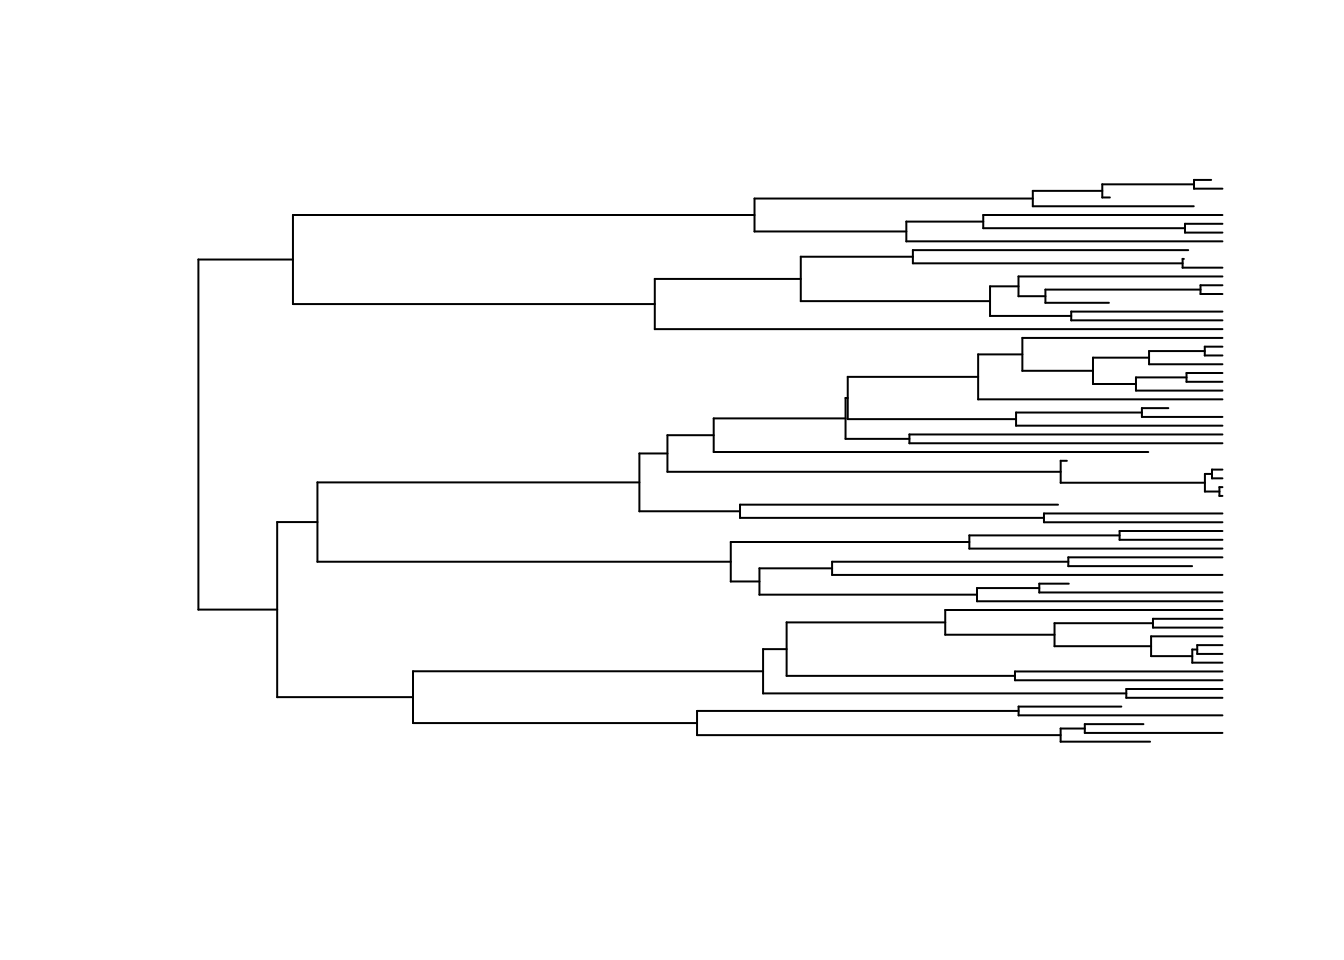
\includegraphics{treats_manual_files/figure-latex/unnamed-chunk-123-1.pdf}

\hypertarget{EGred_spec}{%
\section{Reducing speciation rate after a certain time}\label{EGred_spec}}

For this scenario, we want to generate a birth tree for 6 times units with random speciation rates (i.e.~drawn from a uniform (0.5;1) distribution) which reduces after time 4 through the simulations to a fixed value of 1/3.

First we need to set up the simulation parameters:
* The stopping rule (6 time units)
* The birth-death parameters (speciation randomly drawn between 0.5 and 1)

\begin{Shaded}
\begin{Highlighting}[]
\CommentTok{\#\# Simulation parameters}
\NormalTok{stop\_time\_}\DecValTok{6}\NormalTok{ \textless{}{-}}\StringTok{ }\KeywordTok{list}\NormalTok{(}\DataTypeTok{max.time =} \DecValTok{6}\NormalTok{)}
\NormalTok{random\_speciation \textless{}{-}}\StringTok{ }\KeywordTok{make.bd.params}\NormalTok{(}\DataTypeTok{speciation =}\NormalTok{ runif, }
                                    \DataTypeTok{speciation.args =} \KeywordTok{list}\NormalTok{(}\DataTypeTok{min =} \FloatTok{0.5}\NormalTok{, }\DataTypeTok{max =} \DecValTok{1}\NormalTok{))}
\end{Highlighting}
\end{Shaded}

And our extinction event which triggers after reaching time 4 (\texttt{age.condition(4)}), targets the \texttt{"bd.params"} and modifies the speciation rate to 1/3:

\begin{Shaded}
\begin{Highlighting}[]
\CommentTok{\#\# Reducing speciation after reaching time 4}
\NormalTok{reduced.speciation \textless{}{-}}\StringTok{ }\KeywordTok{make.events}\NormalTok{(}
                      \DataTypeTok{condition =} \KeywordTok{age.condition}\NormalTok{(}\DecValTok{4}\NormalTok{),}
                      \DataTypeTok{target =} \StringTok{"bd.params"}\NormalTok{,}
                      \DataTypeTok{modification =} \KeywordTok{bd.params.update}\NormalTok{(}\DataTypeTok{speciation =} \DecValTok{1}\OperatorTok{/}\DecValTok{3}\NormalTok{))}
\end{Highlighting}
\end{Shaded}

Once these parameters are defined, we can run the simulations and plot the results.
We can contrast the results with the scenario without an event (but same random seed):

\begin{Shaded}
\begin{Highlighting}[]
\CommentTok{\#\# No event}
\KeywordTok{set.seed}\NormalTok{(}\DecValTok{42}\NormalTok{)}
\NormalTok{no\_event \textless{}{-}}\StringTok{ }\KeywordTok{treats}\NormalTok{(}\DataTypeTok{stop.rule =}\NormalTok{ stop\_time\_}\DecValTok{6}\NormalTok{,}
                 \DataTypeTok{bd.params =}\NormalTok{ random\_speciation)}

\CommentTok{\#\# Reduced speciation event}
\KeywordTok{set.seed}\NormalTok{(}\DecValTok{42}\NormalTok{)}
\NormalTok{reduced\_speciation\_event \textless{}{-}}\StringTok{ }\KeywordTok{treats}\NormalTok{(}\DataTypeTok{stop.rule =}\NormalTok{ stop\_time\_}\DecValTok{6}\NormalTok{,}
                                 \DataTypeTok{bd.params =}\NormalTok{ random\_speciation,}
                                 \DataTypeTok{events =}\NormalTok{ reduced.speciation)}

\CommentTok{\#\# Plot both trees}
\KeywordTok{par}\NormalTok{(}\DataTypeTok{mfrow =} \KeywordTok{c}\NormalTok{(}\DecValTok{1}\NormalTok{, }\DecValTok{2}\NormalTok{))}
\KeywordTok{plot}\NormalTok{(no\_event, }\DataTypeTok{main =} \StringTok{"No event"}\NormalTok{, }\DataTypeTok{show.tip.label =} \OtherTok{FALSE}\NormalTok{)}
\KeywordTok{axisPhylo}\NormalTok{()}
\KeywordTok{plot}\NormalTok{(reduced\_speciation\_event, }
     \DataTypeTok{main =} \StringTok{"Reduced speciation after time 5"}\NormalTok{, }
     \DataTypeTok{show.tip.label =} \OtherTok{FALSE}\NormalTok{)}
\KeywordTok{axisPhylo}\NormalTok{()}
\end{Highlighting}
\end{Shaded}

\includegraphics{treats_manual_files/figure-latex/unnamed-chunk-126-1.pdf}

\hypertarget{EG_change_trait}{%
\section{Changing the trait process after some time}\label{EG_change_trait}}

For this scenario, we want to generate a pure birth tree with a one dimensional Brownian Motion trait for 5 time units which then changes to an OU process.

First we need to set up the simulation parameters:
* The stopping rule (6 time units)
* The birth-death parameters (speciation rate of 1)

\begin{Shaded}
\begin{Highlighting}[]
\CommentTok{\#\# Simulation parameters}
\NormalTok{stop\_time\_}\DecValTok{6}\NormalTok{ \textless{}{-}}\StringTok{ }\KeywordTok{list}\NormalTok{(}\DataTypeTok{max.time =} \DecValTok{6}\NormalTok{)}
\NormalTok{speciation\_}\DecValTok{1}\NormalTok{ \textless{}{-}}\StringTok{ }\KeywordTok{make.bd.params}\NormalTok{(}\DataTypeTok{speciation =} \DecValTok{1}\NormalTok{)}
\end{Highlighting}
\end{Shaded}

Then set up our trait which is a one dimensional Brownian Motion

\begin{Shaded}
\begin{Highlighting}[]
\CommentTok{\#\# Trait}
\NormalTok{simple\_bm\_trait \textless{}{-}}\StringTok{ }\KeywordTok{make.traits}\NormalTok{(}\DataTypeTok{n =} \DecValTok{1}\NormalTok{, }\DataTypeTok{process =}\NormalTok{ BM.process)}
\end{Highlighting}
\end{Shaded}

And our event which triggers after reaching time 5 (\texttt{age.condition(5)}), targets the \texttt{"traits"} and modifies the process to \texttt{OU.process}.

\begin{Shaded}
\begin{Highlighting}[]
\CommentTok{\#\# Create an event to change the trait process}
\NormalTok{change.process.to.OU \textless{}{-}}\StringTok{ }\KeywordTok{make.events}\NormalTok{(}
                  \DataTypeTok{condition    =} \KeywordTok{age.condition}\NormalTok{(}\DecValTok{5}\NormalTok{),}
                  \DataTypeTok{target       =} \StringTok{"traits"}\NormalTok{,}
                  \DataTypeTok{modification =} \KeywordTok{traits.update}\NormalTok{(}\DataTypeTok{process =}\NormalTok{ OU.process))}
\end{Highlighting}
\end{Shaded}

Once these parameters are defined, we can run the simulations and plot the results.
We can contrast the results with the scenario without an event (but same random seed):

\begin{Shaded}
\begin{Highlighting}[]
\CommentTok{\#\# Run the simulations without change}
\KeywordTok{set.seed}\NormalTok{(}\DecValTok{1}\NormalTok{)}
\NormalTok{no\_change \textless{}{-}}\StringTok{ }\KeywordTok{treats}\NormalTok{(}\DataTypeTok{stop.rule =}\NormalTok{ stop\_time\_}\DecValTok{6}\NormalTok{,}
                  \DataTypeTok{bd.params =}\NormalTok{ speciation\_}\DecValTok{1}\NormalTok{,}
                  \DataTypeTok{traits    =}\NormalTok{ simple\_bm\_trait)}
\CommentTok{\#\# Run the simulations with change}
\KeywordTok{set.seed}\NormalTok{(}\DecValTok{1}\NormalTok{)}
\NormalTok{process\_change \textless{}{-}}\StringTok{ }\KeywordTok{treats}\NormalTok{(}\DataTypeTok{stop.rule =}\NormalTok{ stop\_time\_}\DecValTok{6}\NormalTok{,}
                       \DataTypeTok{bd.params =}\NormalTok{ speciation\_}\DecValTok{1}\NormalTok{,}
                       \DataTypeTok{traits    =}\NormalTok{ simple\_bm\_trait,}
                       \DataTypeTok{events    =}\NormalTok{ change.process.to.OU)}
\CommentTok{\#\# Plot the results}
\KeywordTok{par}\NormalTok{(}\DataTypeTok{mfrow =} \KeywordTok{c}\NormalTok{(}\DecValTok{1}\NormalTok{,}\DecValTok{2}\NormalTok{))}
\KeywordTok{plot}\NormalTok{(no\_change, }\DataTypeTok{ylim =} \KeywordTok{c}\NormalTok{(}\OperatorTok{{-}}\DecValTok{7}\NormalTok{, }\DecValTok{7}\NormalTok{))}
\KeywordTok{plot}\NormalTok{(process\_change, }\DataTypeTok{ylim =} \KeywordTok{c}\NormalTok{(}\OperatorTok{{-}}\DecValTok{7}\NormalTok{, }\DecValTok{7}\NormalTok{))}
\end{Highlighting}
\end{Shaded}

\includegraphics{treats_manual_files/figure-latex/unnamed-chunk-130-1.pdf}

\hypertarget{EG_change_correlation}{%
\section{Changing trait correlation after reaching a trait value}\label{EG_change_correlation}}

For this scenario, we want to generate a pure birth tree with a 2 dimensional Brownian Motion trait with a strict correlation between the two dimensions (1:1) that loosen up when a taxa reaches an absolute value of 2.

First we need to set up the simulation parameters:
* The stopping rule (100 taxa)
* The birth-death parameters (speciation rate of 1)

\begin{Shaded}
\begin{Highlighting}[]
\CommentTok{\#\# Set the parameters}
\NormalTok{stop\_taxa\_}\DecValTok{100}\NormalTok{ \textless{}{-}}\StringTok{ }\KeywordTok{list}\NormalTok{(}\DataTypeTok{max.taxa =} \DecValTok{100}\NormalTok{)}
\NormalTok{speciation\_}\DecValTok{1}\NormalTok{ \textless{}{-}}\StringTok{ }\KeywordTok{make.bd.params}\NormalTok{(}\DataTypeTok{speciation =} \DecValTok{1}\NormalTok{)}
\end{Highlighting}
\end{Shaded}

Then set up our trait which is a 2 dimensional Brownian Motion with a correlation matrix Sigma ()

\begin{Shaded}
\begin{Highlighting}[]
\CommentTok{\#\# A 2D variance covariance matrix}
\NormalTok{cor\_matrix \textless{}{-}}\StringTok{ }\KeywordTok{matrix}\NormalTok{(}\DecValTok{1}\NormalTok{, }\DecValTok{2}\NormalTok{, }\DecValTok{2}\NormalTok{)}

\CommentTok{\#\# A correlated 2D Brownian Motion}
\NormalTok{correlated\_2D\_BM \textless{}{-}}\StringTok{ }\KeywordTok{make.traits}\NormalTok{(}\DataTypeTok{n =} \DecValTok{2}\NormalTok{, }\DataTypeTok{process =}\NormalTok{ BM.process,}
                      \DataTypeTok{process.args =} \KeywordTok{list}\NormalTok{(}\DataTypeTok{Sigma =}\NormalTok{ cor\_matrix))}
\end{Highlighting}
\end{Shaded}

And our event which triggers after a taxa gets the trait value 3 (\texttt{trait.condition(3,\ absolute\ =\ TRUE)}), targets the \texttt{"traits"} and modifies the traits correlation

\begin{Shaded}
\begin{Highlighting}[]
\CommentTok{\#\# New correlation}
\NormalTok{new\_cor \textless{}{-}}\StringTok{ }\KeywordTok{matrix}\NormalTok{(}\KeywordTok{c}\NormalTok{(}\DecValTok{10}\NormalTok{,}\DecValTok{3}\NormalTok{,}\DecValTok{3}\NormalTok{,}\DecValTok{2}\NormalTok{),}\DecValTok{2}\NormalTok{,}\DecValTok{2}\NormalTok{)}

\CommentTok{\#\# Event changing a trait correlation}
\NormalTok{correlation.change \textless{}{-}}\StringTok{ }\KeywordTok{make.events}\NormalTok{(}
    \DataTypeTok{condition    =} \KeywordTok{trait.condition}\NormalTok{(}\DecValTok{3}\NormalTok{, }\DataTypeTok{absolute =} \OtherTok{TRUE}\NormalTok{),}
    \DataTypeTok{target       =} \StringTok{"traits"}\NormalTok{,}
    \DataTypeTok{modification =} \KeywordTok{traits.update}\NormalTok{(}\DataTypeTok{process.args =} \KeywordTok{list}\NormalTok{(}\DataTypeTok{Sigma =}\NormalTok{ new\_cor)))}
\end{Highlighting}
\end{Shaded}

Once these parameters are defined, we can run the simulations and plot the results.
We can contrast the results with the scenario without an event (but same random seed):

\begin{Shaded}
\begin{Highlighting}[]
\CommentTok{\#\# Run the simulations}
\KeywordTok{set.seed}\NormalTok{(}\DecValTok{2}\NormalTok{)}
\NormalTok{no\_event \textless{}{-}}\StringTok{ }\KeywordTok{treats}\NormalTok{(}\DataTypeTok{stop.rule =}\NormalTok{ stop\_taxa\_}\DecValTok{100}\NormalTok{,}
                 \DataTypeTok{bd.params =}\NormalTok{ speciation\_}\DecValTok{1}\NormalTok{,}
                 \DataTypeTok{traits    =}\NormalTok{ correlated\_2D\_BM)}
\KeywordTok{set.seed}\NormalTok{(}\DecValTok{2}\NormalTok{)}
\NormalTok{change\_correlation \textless{}{-}}\StringTok{ }\KeywordTok{treats}\NormalTok{(}\DataTypeTok{stop.rule =}\NormalTok{ stop\_taxa\_}\DecValTok{100}\NormalTok{,}
                           \DataTypeTok{bd.params =}\NormalTok{ speciation\_}\DecValTok{1}\NormalTok{,}
                           \DataTypeTok{traits    =}\NormalTok{ correlated\_2D\_BM,}
                           \DataTypeTok{events    =}\NormalTok{ correlation.change)}

\CommentTok{\#\# Visual testing}
\KeywordTok{par}\NormalTok{(}\DataTypeTok{mfrow =} \KeywordTok{c}\NormalTok{(}\DecValTok{1}\NormalTok{,}\DecValTok{2}\NormalTok{))}
\KeywordTok{plot}\NormalTok{(no\_event, }\DataTypeTok{trait =} \KeywordTok{c}\NormalTok{(}\DecValTok{1}\NormalTok{,}\DecValTok{2}\NormalTok{), }\DataTypeTok{main =} \StringTok{"Strict correlation"}\NormalTok{)}
\KeywordTok{plot}\NormalTok{(change\_correlation, }\DataTypeTok{trait =} \KeywordTok{c}\NormalTok{(}\DecValTok{1}\NormalTok{,}\DecValTok{2}\NormalTok{), }\DataTypeTok{main =} \StringTok{"Loosened correlation"}\NormalTok{)}
\end{Highlighting}
\end{Shaded}

\includegraphics{treats_manual_files/figure-latex/unnamed-chunk-134-1.pdf}

And we can visualise this change through time:

\begin{Shaded}
\begin{Highlighting}[]
\CommentTok{\#\# 3D plot}
\KeywordTok{plot}\NormalTok{(change\_correlation, }\DataTypeTok{trait =} \KeywordTok{c}\NormalTok{(}\DecValTok{1}\OperatorTok{:}\DecValTok{2}\NormalTok{), }\DataTypeTok{use.3D =} \OtherTok{TRUE}\NormalTok{)}
\KeywordTok{rglwidget}\NormalTok{()}
\end{Highlighting}
\end{Shaded}

\begin{verbatim}
## Warning in snapshot3d(scene = x, width = width, height = height): webshot =
## TRUE requires the webshot2 package and Chrome browser; using rgl.snapshot()
## instead
\end{verbatim}

\begin{verbatim}
## Warning in rgl.snapshot(filename, fmt, top): this build of rgl does not support
## snapshots
\end{verbatim}

\includegraphics[width=6.5in]{../../../../../../tmp/RtmpcKuqE6/file37eb202f55d4}

\hypertarget{EG_change_modif}{%
\section{Event for changing a modifier: extinction event increase for species with negative values}\label{EG_change_modif}}

For this scenario, we want to generate a pure birth tree with a one dimensional Brownian Motion trait for 4 time units.
After 3 time units, we want the speciation rule to increase for species which ancestors have a negative trait value.

First we need to set up the simulation parameters:
* The stopping rule (5 time units)
* The birth-death parameters (speciation rate of 1)

\begin{Shaded}
\begin{Highlighting}[]
\CommentTok{\#\# Set the parameters}
\NormalTok{stop\_time\_}\DecValTok{4}\NormalTok{ \textless{}{-}}\StringTok{ }\KeywordTok{list}\NormalTok{(}\DataTypeTok{max.time =} \DecValTok{4}\NormalTok{)}
\NormalTok{speciation\_}\DecValTok{1}\NormalTok{ \textless{}{-}}\StringTok{ }\KeywordTok{make.bd.params}\NormalTok{(}\DataTypeTok{speciation =} \DecValTok{1}\NormalTok{)}
\end{Highlighting}
\end{Shaded}

Then set up our trait which is a one dimensional Brownian Motion

\begin{Shaded}
\begin{Highlighting}[]
\CommentTok{\#\# Trait}
\NormalTok{simple\_bm\_trait \textless{}{-}}\StringTok{ }\KeywordTok{make.traits}\NormalTok{(}\DataTypeTok{n =} \DecValTok{1}\NormalTok{, }\DataTypeTok{process =}\NormalTok{ BM.process)}
\end{Highlighting}
\end{Shaded}

And a modifier that is the default birth-death algorithm rules

\begin{Shaded}
\begin{Highlighting}[]
\CommentTok{\#\# birth{-}death rules (default)}
\NormalTok{default\_modifiers \textless{}{-}}\StringTok{ }\KeywordTok{make.modifiers}\NormalTok{()}
\end{Highlighting}
\end{Shaded}

And our extinction event which triggers after reaching time 3 (\texttt{age.condition(3)}), targets the \texttt{"modifiers"} and modifies birth-death rule as follows:
* When a species is descendant from a parent with a negative trait value (\texttt{negative.trait.condition});
* Then increase your chances of going extinct by +1 (\texttt{increase.extinction.1})

\begin{Shaded}
\begin{Highlighting}[]
\CommentTok{\#\# New condition and new modifier (increasing speciation if trait is negative)}
\NormalTok{negative.trait.condition \textless{}{-}}\StringTok{ }\ControlFlowTok{function}\NormalTok{(trait.values, lineage) \{}
    \KeywordTok{return}\NormalTok{(}\KeywordTok{parent.traits}\NormalTok{(trait.values, lineage) }\OperatorTok{\textless{}}\StringTok{ }\DecValTok{0}\NormalTok{)}
\NormalTok{\}}
\NormalTok{increase.extinction}\FloatTok{.1}\NormalTok{ \textless{}{-}}\StringTok{ }\ControlFlowTok{function}\NormalTok{(x, trait.values, lineage) \{}
  \KeywordTok{return}\NormalTok{(x }\OperatorTok{+}\StringTok{ }\DecValTok{1}\NormalTok{)}
\NormalTok{\}}

\CommentTok{\#\# Update the modifier}
\NormalTok{change.speciation \textless{}{-}}\StringTok{ }\KeywordTok{make.events}\NormalTok{(}
    \DataTypeTok{condition    =} \KeywordTok{age.condition}\NormalTok{(}\DecValTok{3}\NormalTok{),}
    \DataTypeTok{target       =} \StringTok{"modifiers"}\NormalTok{,}
    \DataTypeTok{modification =} \KeywordTok{modifiers.update}\NormalTok{(}\DataTypeTok{speciation =}\NormalTok{ speciation,}
                                    \DataTypeTok{condition  =}\NormalTok{ negative.trait.condition,}
                                    \DataTypeTok{modify     =}\NormalTok{ increase.extinction}\FloatTok{.1}\NormalTok{))}
\end{Highlighting}
\end{Shaded}

Once these parameters are defined, we can run the simulations and plot the results.
We can contrast the results with the scenario without an event (but same random seed):

\begin{Shaded}
\begin{Highlighting}[]
\KeywordTok{set.seed}\NormalTok{(}\DecValTok{4}\NormalTok{)}
\NormalTok{no\_event \textless{}{-}}\StringTok{ }\KeywordTok{treats}\NormalTok{(}\DataTypeTok{stop.rule =}\NormalTok{ stop\_time\_}\DecValTok{4}\NormalTok{,}
                 \DataTypeTok{bd.params =}\NormalTok{ speciation\_}\DecValTok{1}\NormalTok{,}
                 \DataTypeTok{traits    =}\NormalTok{ simple\_bm\_trait,}
                 \DataTypeTok{modifiers =}\NormalTok{ default\_modifiers)}
\KeywordTok{set.seed}\NormalTok{(}\DecValTok{4}\NormalTok{)}
\NormalTok{change\_spec \textless{}{-}}\StringTok{ }\KeywordTok{treats}\NormalTok{(}\DataTypeTok{stop.rule =}\NormalTok{ stop\_time\_}\DecValTok{4}\NormalTok{,}
                    \DataTypeTok{bd.params =}\NormalTok{ speciation\_}\DecValTok{1}\NormalTok{,}
                    \DataTypeTok{traits    =}\NormalTok{ simple\_bm\_trait,}
                    \DataTypeTok{modifiers =}\NormalTok{ default\_modifiers,}
                    \DataTypeTok{events    =}\NormalTok{ change.speciation)}

\CommentTok{\#\# Visualise the results}
\KeywordTok{par}\NormalTok{(}\DataTypeTok{mfrow =} \KeywordTok{c}\NormalTok{(}\DecValTok{1}\NormalTok{,}\DecValTok{2}\NormalTok{))}
\KeywordTok{plot}\NormalTok{(no\_event, }\DataTypeTok{main =} \StringTok{"No event"}\NormalTok{)}
\KeywordTok{plot}\NormalTok{(change\_spec, }\DataTypeTok{main =} \StringTok{"Increase extinction for negative}\CharTok{\textbackslash{}n}\StringTok{traits after time 3"}\NormalTok{)}
\end{Highlighting}
\end{Shaded}

\includegraphics{treats_manual_files/figure-latex/unnamed-chunk-140-1.pdf}

\hypertarget{EG_modify_brlen}{%
\section{Changing branch length when reaching n taxa}\label{EG_modify_brlen}}

For this scenario, we want to generate a pure birth tree until reaching 100 taxa.
After reaching 30 taxa we want branch length growth to increase 50 folds.

First we need to set up the simulation parameters:
* The stopping rule (100 taxa)
* The birth-death parameters (speciation rate of 1)

\begin{Shaded}
\begin{Highlighting}[]
\CommentTok{\#\# Set the parameters}
\NormalTok{stop\_taxa\_}\DecValTok{100}\NormalTok{\textless{}{-}}\StringTok{ }\KeywordTok{list}\NormalTok{(}\DataTypeTok{max.taxa =} \DecValTok{100}\NormalTok{)}
\NormalTok{speciation\_}\DecValTok{1}\NormalTok{ \textless{}{-}}\StringTok{ }\KeywordTok{make.bd.params}\NormalTok{(}\DataTypeTok{speciation =} \DecValTok{1}\NormalTok{)}
\end{Highlighting}
\end{Shaded}

Then a modifier that is the default birth-death algorithm rules

\begin{Shaded}
\begin{Highlighting}[]
\CommentTok{\#\# birth{-}death rules (default)}
\NormalTok{default\_modifiers \textless{}{-}}\StringTok{ }\KeywordTok{make.modifiers}\NormalTok{()}
\end{Highlighting}
\end{Shaded}

And event which triggers after reaching 30 taxa (\texttt{taxa.condition(30)}), targets the \texttt{"modifiers"} and modifies the branch length generation rule to a 50 fold increase (\texttt{increase.50.folds})

\begin{Shaded}
\begin{Highlighting}[]
\CommentTok{\#\# Multiplying branch length 50 folds}
\NormalTok{increase.}\FloatTok{50.}\NormalTok{folds \textless{}{-}}\StringTok{ }\ControlFlowTok{function}\NormalTok{(x, trait.values, lineage) \{}
  \KeywordTok{return}\NormalTok{(x }\OperatorTok{*}\StringTok{ }\DecValTok{50}\NormalTok{)}
\NormalTok{\}}
\CommentTok{\#\# Event for increasing branch length after reaching 30 taxa}
\NormalTok{increase\_brlen \textless{}{-}}\StringTok{ }\KeywordTok{make.events}\NormalTok{(}
                  \DataTypeTok{condition =} \KeywordTok{taxa.condition}\NormalTok{(}\DecValTok{30}\NormalTok{),}
                  \DataTypeTok{target =} \StringTok{"modifiers"}\NormalTok{,}
                  \DataTypeTok{modification =} \KeywordTok{modifiers.update}\NormalTok{(}
                                    \DataTypeTok{branch.length =}\NormalTok{ branch.length,}
                                    \DataTypeTok{modify  =}\NormalTok{ increase.}\FloatTok{50.}\NormalTok{folds))}
\end{Highlighting}
\end{Shaded}

Once these parameters are defined, we can run the simulations and plot the results.
We can contrast the results with the scenario without an event (but same random seed):

\begin{Shaded}
\begin{Highlighting}[]
\CommentTok{\#\# Run the simulations}
\KeywordTok{set.seed}\NormalTok{(}\DecValTok{5}\NormalTok{)}
\NormalTok{no\_event \textless{}{-}}\StringTok{ }\KeywordTok{treats}\NormalTok{(}\DataTypeTok{stop.rule =}\NormalTok{ stop\_taxa\_}\DecValTok{100}\NormalTok{,}
                 \DataTypeTok{bd.params =}\NormalTok{ speciation\_}\DecValTok{1}\NormalTok{,}
                 \DataTypeTok{modifiers =}\NormalTok{ default\_modifiers)}
\KeywordTok{set.seed}\NormalTok{(}\DecValTok{5}\NormalTok{)}
\NormalTok{increased\_brlen \textless{}{-}}\StringTok{ }\KeywordTok{treats}\NormalTok{(}\DataTypeTok{stop.rule =}\NormalTok{ stop\_taxa\_}\DecValTok{100}\NormalTok{,}
                        \DataTypeTok{bd.params =}\NormalTok{ speciation\_}\DecValTok{1}\NormalTok{,}
                        \DataTypeTok{modifiers =}\NormalTok{ default\_modifiers,}
                        \DataTypeTok{events =}\NormalTok{ increase\_brlen)}

\CommentTok{\#\# Visualise the results}
\KeywordTok{par}\NormalTok{(}\DataTypeTok{mfrow =} \KeywordTok{c}\NormalTok{(}\DecValTok{1}\NormalTok{,}\DecValTok{2}\NormalTok{))}
\KeywordTok{plot}\NormalTok{(no\_event, }\DataTypeTok{main =} \StringTok{"No event"}\NormalTok{, }\DataTypeTok{show.tip.label =} \OtherTok{FALSE}\NormalTok{)}
\KeywordTok{plot}\NormalTok{(increased\_brlen, }\DataTypeTok{main =} \StringTok{"Increase branch length}\CharTok{\textbackslash{}n}\StringTok{after 30 taxa"}\NormalTok{,}
    \DataTypeTok{show.tip.label =} \OtherTok{FALSE}\NormalTok{)}
\end{Highlighting}
\end{Shaded}

\includegraphics{treats_manual_files/figure-latex/unnamed-chunk-144-1.pdf}

\hypertarget{EG_founding_purebirth}{%
\section{Founding event: generating a subtree with no fossils}\label{EG_founding_purebirth}}

For this scenario, we want to generate a birth-death tree for 4 time units.
After reaching 10 taxa, one random taxa will give birth to a sub-tree that is a pure birth tree (no extinction).

First we need to set up the simulation parameters:
* The stopping rule (5 time units)
* The birth-death parameters (speciation rate of 1 and extinction of 0.2)

\begin{Shaded}
\begin{Highlighting}[]
\CommentTok{\#\# Set up parameters}
\NormalTok{stop\_time\_}\DecValTok{4}\NormalTok{ \textless{}{-}}\StringTok{ }\KeywordTok{list}\NormalTok{(}\DataTypeTok{max.time =} \DecValTok{4}\NormalTok{)}
\NormalTok{spec\_}\DecValTok{1}\NormalTok{\_ext\_}\DecValTok{02}\NormalTok{ \textless{}{-}}\StringTok{ }\KeywordTok{make.bd.params}\NormalTok{(}\DataTypeTok{speciation =} \DecValTok{1}\NormalTok{, }\DataTypeTok{extinction =} \FloatTok{0.2}\NormalTok{)}
\end{Highlighting}
\end{Shaded}

And our event which triggers after reaching 10 taxa (\texttt{taxa.condition(10)}), and generates a subtree (``founding'') that is a pure birth tree (no extinction and speciation rate of 2).

\begin{Shaded}
\begin{Highlighting}[]
\CommentTok{\#\# Setting the pure{-}birth parameters}
\NormalTok{speciation\_}\DecValTok{2}\NormalTok{ \textless{}{-}}\StringTok{ }\KeywordTok{make.bd.params}\NormalTok{(}\DataTypeTok{speciation =} \DecValTok{2}\NormalTok{)}

\CommentTok{\#\# Events that generate a new process (founding effects)}
\NormalTok{founding\_event \textless{}{-}}\StringTok{ }\KeywordTok{make.events}\NormalTok{(}
                  \DataTypeTok{condition =} \KeywordTok{taxa.condition}\NormalTok{(}\DecValTok{10}\NormalTok{),}
                  \DataTypeTok{target  =} \StringTok{"founding"}\NormalTok{,}
                  \DataTypeTok{modification =} \KeywordTok{founding.event}\NormalTok{(}
                                    \DataTypeTok{bd.params =}\NormalTok{ speciation\_}\DecValTok{2}\NormalTok{),}
                  \DataTypeTok{additional.args =} \KeywordTok{list}\NormalTok{(}\DataTypeTok{prefix =} \StringTok{"founding\_"}\NormalTok{))}
\end{Highlighting}
\end{Shaded}

\begin{quote}
Note we are prodviding an additional argument \texttt{prefix} here so that we can track which species are part of the sub tree for colouring them down the line.
\end{quote}

Once these parameters are defined, we can run the simulations and plot the results:

\begin{Shaded}
\begin{Highlighting}[]
\CommentTok{\#\# Simulations}
\KeywordTok{set.seed}\NormalTok{(}\DecValTok{11}\NormalTok{)}
\NormalTok{founding\_tree \textless{}{-}}\StringTok{ }\KeywordTok{treats}\NormalTok{(}\DataTypeTok{stop.rule =}\NormalTok{ stop\_time\_}\DecValTok{4}\NormalTok{,}
                      \DataTypeTok{bd.params =}\NormalTok{ spec\_}\DecValTok{1}\NormalTok{\_ext\_}\DecValTok{02}\NormalTok{,}
                      \DataTypeTok{events =}\NormalTok{ founding\_event)}

\CommentTok{\#\# Selecting the edges colours}
\NormalTok{tip\_values \textless{}{-}}\StringTok{ }\KeywordTok{rep}\NormalTok{(}\StringTok{"black"}\NormalTok{, }\KeywordTok{Ntip}\NormalTok{(founding\_tree))}
\NormalTok{tip\_values[}\KeywordTok{grep}\NormalTok{(}\StringTok{"founding\_"}\NormalTok{, founding\_tree}\OperatorTok{$}\NormalTok{tip.label)] \textless{}{-}}\StringTok{ "orange"}
\NormalTok{edge\_colors \textless{}{-}}\StringTok{ }\KeywordTok{match.tip.edge}\NormalTok{(tip\_values, founding\_tree, }\DataTypeTok{replace.na =} \StringTok{"black"}\NormalTok{)}

\CommentTok{\#\# Plotting the results}
\KeywordTok{plot}\NormalTok{(founding\_tree, }\DataTypeTok{show.tip.label =} \OtherTok{FALSE}\NormalTok{, }\DataTypeTok{edge.color =}\NormalTok{ edge\_colors)}
\end{Highlighting}
\end{Shaded}

\includegraphics{treats_manual_files/figure-latex/unnamed-chunk-147-1.pdf}

\hypertarget{EG_founding_traits}{%
\section{Founding event: generating a subtree a different process}\label{EG_founding_traits}}

For this scenario, we want to generate a birth-death tree with a one dimensional Brownian Motion trait for 6 time units.
After a taxon reaches the value 3 or higher, it gives birth to a sub-tree that generates an OU trait with a long-term mean at the value 3.

First we need to set up the simulation parameters:
* The stopping rule (6 time units)
* The birth-death parameters (speciation rate of 1 and extinction of 1/3)

\begin{Shaded}
\begin{Highlighting}[]
\CommentTok{\#\# The tree parameters}
\NormalTok{stop\_time\_}\DecValTok{6}\NormalTok{ \textless{}{-}}\StringTok{ }\KeywordTok{list}\NormalTok{(}\DataTypeTok{max.time =} \DecValTok{6}\NormalTok{)}
\NormalTok{speciation\_}\DecValTok{1}\NormalTok{\_extinction\_}\DecValTok{03}\NormalTok{ \textless{}{-}}\StringTok{ }\KeywordTok{make.bd.params}\NormalTok{(}\DataTypeTok{speciation =} \DecValTok{1}\NormalTok{,}
                                             \DataTypeTok{extinction =} \FloatTok{0.3}\NormalTok{)}
\end{Highlighting}
\end{Shaded}

Then set up our trait which is a one dimensional Brownian Motion

\begin{Shaded}
\begin{Highlighting}[]
\CommentTok{\#\# Trait}
\NormalTok{simple\_bm\_trait \textless{}{-}}\StringTok{ }\KeywordTok{make.traits}\NormalTok{(}\DataTypeTok{n =} \DecValTok{1}\NormalTok{, }\DataTypeTok{process =}\NormalTok{ BM.process)}
\end{Highlighting}
\end{Shaded}

When a taxa reaches the value 3 \texttt{trait.condition}, it generates a pure birth tree (\texttt{speciation\ =\ 2}) with an OU trait with the long-term mean value 3.

\begin{Shaded}
\begin{Highlighting}[]
\CommentTok{\#\# The OU trait with a long{-}term mean value of 3}
\NormalTok{OU\_}\DecValTok{3}\NormalTok{ \textless{}{-}}\StringTok{ }\KeywordTok{make.traits}\NormalTok{(}\DataTypeTok{process =}\NormalTok{ OU.process,}
                    \DataTypeTok{start =} \DecValTok{3}\NormalTok{, }\DataTypeTok{process.args =} \KeywordTok{list}\NormalTok{(}\DataTypeTok{optimum =} \DecValTok{3}\NormalTok{))}
\CommentTok{\#\# The pure birth parameters}
\NormalTok{speciation\_}\DecValTok{2}\NormalTok{ \textless{}{-}}\StringTok{ }\KeywordTok{make.bd.params}\NormalTok{(}\DataTypeTok{speciation =} \DecValTok{2}\NormalTok{)}

\CommentTok{\#\# The founding event}
\NormalTok{new\_OU\_trait \textless{}{-}}\StringTok{ }\KeywordTok{make.events}\NormalTok{(}
                    \DataTypeTok{condition    =} \KeywordTok{trait.condition}\NormalTok{(}\DecValTok{3}\NormalTok{, }\DataTypeTok{condition =} \StringTok{\textasciigrave{}}\DataTypeTok{\textgreater{}=}\StringTok{\textasciigrave{}}\NormalTok{),}
                    \DataTypeTok{target       =} \StringTok{"founding"}\NormalTok{,}
                    \DataTypeTok{modification =} \KeywordTok{founding.event}\NormalTok{(}
                                    \DataTypeTok{bd.params =}\NormalTok{ speciation\_}\DecValTok{2}\NormalTok{,}
                                    \DataTypeTok{traits    =}\NormalTok{ OU\_}\DecValTok{3}\NormalTok{))}
\end{Highlighting}
\end{Shaded}

Once these parameters are defined, we can run the simulations and plot the results:

\begin{Shaded}
\begin{Highlighting}[]
\CommentTok{\#\# Simulating the tree}
\KeywordTok{set.seed}\NormalTok{(}\DecValTok{1}\NormalTok{)}
\NormalTok{founding\_tree \textless{}{-}}\StringTok{ }\KeywordTok{treats}\NormalTok{(}\DataTypeTok{stop.rule =}\NormalTok{ stop\_time\_}\DecValTok{6}\NormalTok{,}
                      \DataTypeTok{bd.params =}\NormalTok{ speciation\_}\DecValTok{1}\NormalTok{\_extinction\_}\DecValTok{03}\NormalTok{,}
                      \DataTypeTok{traits =}\NormalTok{ simple\_bm\_trait,}
                      \DataTypeTok{events =}\NormalTok{ new\_OU\_trait)}
\KeywordTok{plot}\NormalTok{(founding\_tree)}
\end{Highlighting}
\end{Shaded}

\includegraphics{treats_manual_files/figure-latex/unnamed-chunk-151-1.pdf}

  \bibliography{../references.bib}

\end{document}
